%=============================================================================
% Cursus Onderzoekstechnieken HOGENT toegepaste informatica
%=============================================================================

\documentclass{hogent-report}

%-----------------------------------------------------------------------------
% Packages en instellingen specifiek voor dit document
%-----------------------------------------------------------------------------

%% Titelpagina
\usepackage{hogent-titlepage-image}

%% Figuren
\usepackage{pgfplotstable}
\usepackage{pgfplots}
\pgfplotsset{compat=1.13}
\usetikzlibrary{arrows,shapes,backgrounds,positioning,shadows}
\usetikzlibrary{pgfplots.statistics}

\pgfmathdeclarefunction{gauss}{2}{%
  \pgfmathparse{1/(#2*sqrt(2*pi))*exp(-((x-#1)^2)/(2*#2^2))}%
}

%% Titel
\title{Cursus~\\Onderzoekstechnieken}
\author{Dr. Jens Buysse, Wim {De Bruyn}, Pieter-Jan Maenhaut , Bert {Van Vreckem}}
\date{Academiejaar 2019-2020}

\hypersetup{
  pdftitle={\thetitle},
  pdfauthor={\theauthor}
}

\begin{document}

\inserttitlepage{achtergrond-ozt.png}

%-----------------------------------------------------------------------------
% Copyright
%-----------------------------------------------------------------------------

\newpage

\thispagestyle{empty}

\vspace*{20cm}

\noindent Copyright \copyright\ 2015-{\the\year} Jens Buysse % Copyright notice

\noindent \textsc{www.hogent.be} % URL

\noindent \textit{Gegenereerd op \today} % Printing/edition date

%-----------------------------------------------------------------------------
% Inhoudstafel
%-----------------------------------------------------------------------------

\usechapterimagefalse
\tableofcontents % Print the table of contents itself

\cleardoublepage % Forces the first chapter to start on an odd page so it's on the right

\def\R{\mathbb{R}}

%-----------------------------------------------------------------------------
% Corpus
%-----------------------------------------------------------------------------



\chapter*{Voorwoord}
Deze cursus werd geschreven in het kader van de lessenreeks Onderzoekstechnieken aan de Hogeschool Gent. Ik wil hierbij gebruik maken om volgende mensen te bedanken bij het nakijken en verbeteren van de cursus.
\begin{itemize}
	\item C\'edric Berlez
	\item J\"urgen Van Meerhaeghe
	\item Gianni Stubbe
	\item Jelle Elaut
	\item Thijs Van Der Burgt
	\item Lotte Potth\'e
	\item \"Ozg\"ur Akin
	\item Cedric De Vylder
\end{itemize}

\bigskip \bigskip
{\raggedleft	% Lijn rechts uit
Jens Buysse\\
10 januari 2020\\
}


\chapter{Aan de slag}
\label{ch:aan-de-slag}

\section{Studiewijzer}

De studiewijzer geeft een overzicht van de belangrijkste informatie over deze cursus, o.a.~leerdoelen, lesmateriaal, weekplanning en leeraanwijzingen. Lees alles aandachtig door!

\subsection{Doel en plaats van de cursus in het curriculum}

Deze cursus is een inleiding op wat tegenwoordig vaak \emph{data science} genoemd wordt. Het doel is om je wegwijs te maken in het correct verzamelen, verwerken en analyseren van numerieke data en daar een onderbouwd onderzoeksverslag over te schrijven.

In de eerste plaats is dit een voorbereiding op de bachelorproef, waar je deze technieken in de praktijk zal moeten omzetten. Maar ook na je afstuderen blijft de kennis die je in deze cursus opdoet waardevol. Succesvolle bedrijven nemen beslissingen, niet op basis van buikgevoel of intuïtie, maar door het verzamelen en analyseren van data. Aan de hand van de technieken die hier toegelicht worden, heb je voldoende achtergrond om vragen te beantwoorden als:

\begin{itemize}
  \item Is een (web)applicatie snel genoeg voor de gebruikers? Is de gebruikerservaring consistent, of zit er grote variatie op responstijden?
  \item Als je twee systemen moet vergelijken, zij het software of hardware, welke van de twee is het meest performant? Is het verschil tussen beide significant, of kunnen verschillen in de metingen te wijten zijn aan het toeval of andere factoren?
  \item Wanneer moeten aankopen van nieuwe apparatuur (bv.~harde schijven, servers, geheugen, enz.) ingepland worden, op basis van historische gebruiksgegevens?
\end{itemize}

De competenties die je in deze cursus verwerft hebben ook buiten de informatica hun nut. Je leert immers kritisch omgaan met data en informatie, en hoe die correct te analyseren en interpreteren. In het politieke en maatschappelijke debat worden moedwillig beweringen gedaan die aantoonbaar fout zijn of die de waarheid proberen ``om te buigen.'' De term die in dat verband vaak de kop opsteekt is `Fake News'. Een manier om je hiertegen te wapenen is kritisch omgaan met de informatie die verspreid wordt. Daardoor kan vaak de achterliggende reden van die desinformatie duidelijk gemaakt worden.

Statistiek  en data science zijn dan ook onontbeerlijk om (i) te data correct te analyseren en tot onderbouwde conclusies te komen en (ii) zelf onderzoeken uit te voeren waarbij je onderbouwde conclusies de wereld kan in sturen. 

\subsection{Leerdoelen en competenties}

\begin{itemize}
  \item Kan begrippen, formules, stellingen en de uitwerking ervan uit de beschrijvende en inductieve statistiek benoemen en verklaren
  \item Kan formules, stellingen uit de beschrijvende en inductieve statistiek in onderzoeksvraagstukken correct toepassen
  \item Kan data analyseren met statistische software
  \item Kan een gestructureerd wetenschappelijk document schrijven en voorzien van referenties in \LaTeX{}
  \item Kan de wetenschappelijke methode vergelijken met niet-wetenschappelijke onderzoeksmethodes en daarbij voor- en nadelen opsommen 
\end{itemize}

Deze vind je ook terug in de studiefiche.

\subsection{Leerinhoud}

Verder in dit hoofdstuk vind je instructies voor het installeren van de nodige software, en een korte inleiding op het werken met R, een programmeertaal voor data-analyse.

Hoofdstuk~\ref{ch:onderzoeksproces} geeft een inleiding op het verloop van een typisch onderzoeksproces en introduceert enkele basisconcepten van data-analyse, waaronder het nemen van een steekproef uit een populatie, variabelen en meetniveaus.

Hoofdstuk~\ref{ch:analyse1var} behandelt de analyse van een enkele variabele, meer bepaald centrum- en spreidingsmaten, samen met geschikte visualisatietechnieken voor elke soort variabele.

Hoofdstuk ~\ref{ch:centrale-limietstelling} herhaalt kort de stof rond kansverdelingen, waarna de centrale limietstelling aan bod komt met een onmiddelijke toepassing via betrouwbaarheidsintervallen. 

Hoofdstuk~\ref{ch:toetsingsprocedures} gaat hierop verder met de algemene werkwijze voor het voeren van statistische toetsen, en specifiek met toetsen voor uitspraken over het gemiddelde van een populatie: de $z$-toets en de $t$-toets.

Waar de vorige hoofdstukken telkens één variabele apart beschouwden, bekijkt Hoofdstuk~\ref{ch:analyse2var} verschillende technieken om verbanden tussen twee variabelen te leggen, afhankelijk van het variabeletype.

Hoofdstuk~\ref{ch:tijdreeksen} geeft een inleiding op het analyseren van hoe de waarde van een variabele evolueert in de tijd aan de hand van wiskundige modellen die onder bepaalde voorwaarden ook toelaten om voorspellingen te doen.

\subsection{Leermateriaal}

Het belangrijkste leermateriaal voor dit opleidingsonderdeel is deze cursus, die ook de oefeningenopgaven bevat. Die wordt ter beschikking gesteld via Chamilo als PDF. Op Chamilo vind je ook de PDF's met de slides gebruikt tijdens de lessen.

Daarnaast krijgen studenten toegang tot een GitHub-repository met de broncode voor:

\begin{itemize}
  \item Deze cursus
  \item De slides gebruikt tijdens de lessen
  \item Broncodevoorbeelden in R voor alle technieken die in de cursus aan bod komen.
\end{itemize}

\textbf{Errata en wijzigingen} aan de cursus worden in GitHub aangebracht. De PDF's op Chamilo zullen niet noodzakelijk bijgewerkt worden. Studenten kunnen zelf de laatste versies van alle documenten met \LaTeX{} genereren.

De software die nodig is voor dit opleidingsonderdeel is gratis/open source. Instructies voor de installatie kan je vinden in Sectie~\ref{sec:installatie-software}.

\subsection{Werkvormen}

\textbf{Studenten afstandsleren} kunnen vragen stellen tijdens de contactmomenten. Dit zijn echter geen lesmomenten! Het rooster vind je in de Chamilo-cursus ``Informatie voor studenten TILE.''

\textbf{Studenten dagonderwijs} krijgen drie uur per week les, waarvan één uur klassikale instructie en hoorcollege, en twee uur oefeningen en begeleiding bij het groepswerk.

\subsection{Werk- en leeraanwijzingen}

Het opleidingsonderdeel \emph{Onderzoekstechnieken} wordt door veel studenten als moeilijk ervaren. Dat is begrijpelijk, want het onderwerp ligt dan ook buiten de comfortzone van de doorsnee informaticastudent en we weten allemaal dat wiskundige vakken niet de populairste van onze opleiding zijn.

Er zijn twee manieren om hier mee om te gaan. Je kan de weg van de minste weerstand nemen: je concentreren op de vakken die je graag doet en een dag voor het examen de cursus doornemen in de hoop dat je voldoende punten bij elkaar sprokkelt om een tien te halen. De ervaring leert dat deze strategie niet succesvol is, wat blijkt uit het lage slagingspercentage in de eerste zittijd (in academiejaar 2016-2017 was dat ca. 35\% voor het dagonderwijs en 10\% voor afstandsleren). In de tweede zittijd zien we vaak een veel hoger slagingspercentage, wat naar onze mening suggereert dat wanneer je voldoende inspanning levert voor dit vak, het zeker haalbaar is.

Enkele tips om w\'el meteen te slagen voor dit vak:

\begin{itemize}
  \item Kom naar de les en \emph{neem actief nota's}~\parencite{Lundin2020};
  \item Werk ook voor dit vak \emph{buiten de contactmomenten}. Herhaal de geziene theorie en werk oefeningen af waarmee je nog niet klaar was. Noteer zaken die je niet begrijpt of waar je vast zit, en stel je vraag tijdens het eerstvolgende college.
  \item Gebruik goede \emph{leertechnieken}. Je vindt een goed overzicht van leertechnieken waarvan het effect wetenschappelijk aangetoond is via de website van \emph{The Learning Scientists}\footnote{\url{http://www.learningscientists.org/}}.
  \begin{itemize}
    \item \emph{Spaced practice:} Studeer in meerdere kleine sessies (minstens één keer per week) en niet in grote blokken. Blokkeer een vast moment in je weekagenda/lesplanning.
    \item \emph{Retrieval practice:} Neem een leeg blad papier en probeer zoveel mogelijk zaken over een bepaald onderwerp op te schrijven vanuit je herinnering (dus zonder in de cursus te kijken). Controleer dit daarna aan de hand van je lesnota's en in de cursus.
    \item \emph{Elaboration:} Stel jezelf vragen over hoe dingen (bv. formules, toetsingsprocedures \ldots) in elkaar zitten en waarom dat zo is. Overleg met medestudenten. Vraag je lector om meer uitleg indien nodig. Leg verbanden tussen verschillende onderwerpen in de cursus (bv. vergelijk toetsingsprocedures).
    \item \emph{Interleaving:} Wissel onderwerpen af tijdens het studeren.
    \item Gebruik \emph{concrete voorbeelden} om abstracte idee\"en te begrijpen. In de cursus worden reeds enkele voorbeelden gegeven, probeer er zelf andere te bedenken. Overleg met medestudenten en vraag eventueel feedback aan je lector.
    \item \emph{Dual coding:} Combineer woord en beeld, probeer de leerstof die je instudeert visueel voor te stellen.
  \end{itemize}
\end{itemize}

Uiteindelijk komt het er op neer dat je voldoende tijd en inspanning investeert om te studeren voor dit vak.

\subsection{Studiebegeleiding en planning}

Studenten \textbf{afstandsleren} die vragen hebben over de leerstof kunnen in de eerste plaats terecht op het forum in Chamilo. Op de contactmomenten voor afstandsleren is er ook gelegenheid voor het stellen van vragen.

Studenten \textbf{dagonderwijs} kunnen vragen stellen tijdens de werkcolleges of  op het forum.

%In Tabel~\ref{tab:weekplanning} vind je een overzicht van de lesplanning voor het dagonderwijs die ook als leidraad kan dienen voor de studieplanning van studenten afstandsleren.

%\begin{table}
%  \begin{center}
%    \begin{tabular}{cll}
%       \hline
%       \textbf{Week} & \textbf{Theorie}     & \textbf{Oefeningen}            \\
%       \hline
%       1  & Intro, Onderzoeksproces         & Software installeren, \LaTeX{} \\
%       2  & Analyse van 1 variabele         & Wetenschappelijk schrijven     \\
%       3  & Steekproefonderzoek             & Analyse van 1 variabele        \\
%       4  & Steekproefonderzoek             & Steekproefonderzoek            \\
%       5  & Toetsingsprocedures ($z$-toets) & Steekproefonderzoek            \\
%       6  & Toetsingsprocedures ($t$-toets) & Toetsingsprocedures            \\
%       7  & Analyse van 2 variabelen        & Toetsingsprocedures            \\
%      --- & \textbf{Paasvakantie}           & ---                            \\
%       8  & Analyse van 2 variabelen        & Analyse van 2 variabelen       \\
%       9  & $\chi^2$-toets                  & Analyse van 2 variabelen       \\
%      10  & Tijdreeksen                     & $\chi^2$-toets                 \\
%      11  & Toelichting bachelorproef       & Tijdreeksen                    \\
%      12  & Herhaling                       & Herhaling                      \\
%      \hline
%    \end{tabular}
%    \caption[Weekplanning]{Weekplanning van de cursus.}
%    \label{tab:weekplanning}
%  \end{center}
%\end{table}

\subsection{Evaluatie}



\begin{itemize}
  \item Eerste examenperiode:
  \begin{itemize}
    \item 70\% periodegebonden evaluatie: schriftelijk examen, bestaande uit een deel gesloten boek (theorie) en een deel met voorbereiding op pc (oefeningen)
    \item 30\% niet-periodegebonden evaluatie, groepsopdracht: het voeren van een mini-onderzoek in groep, bestaande uit een literatuurstudie, opzetten van een reproduceerbaar experiment, verzamelen van meetgegevens en die statistisch analyseren, en er een verslag over schrijven
  \end{itemize}
  \item Tweede examenperiode:
  \begin{itemize}
    \item 70\% periodegebonden evaluatie: schriftelijk examen, bestaande uit een deel gesloten boek (theorie) en een deel met voorbereiding op pc (oefeningen)
    \item 30\% niet-periodegebonden evaluatie: er wordt geen tweede examenkans georganiseerd voor dit onderdeel. Wanneer een student in de eerste examenkans niet geslaagd was voor het opleidingsonderdeel wordt het resultaat voor de groepsopdracht ongewijzigd overgenomen.
  \end{itemize}
\end{itemize}

\section{Installatie software}
\label{sec:installatie-software}

Voor de cursus onderzoekstechnieken maak je gebruik van verschillende softwarepakketten. Hier vind je wat uitleg over de installatie en hoe je er mee aan de slag kan.

\begin{itemize}
  \item Git client (versiebeheersysteem);
  \item \LaTeX{} compiler;
  \item \LaTeX{} editor;
  \item Jabref (bibliografische databank);
  \item R (statistische analysesoftware);
  \item Rstudio (IDE voor R);
  \item Lettertypes voor de HOGENT-huisstijl.
\end{itemize}

Sommige van deze applicaties nemen veel schijfruimte in, dus zorg dat je voldoende ruimte vrij hebt.

In vele andere cursussen rond statistiek of onderzoekstechnieken wordt gebruik gemaakt van commerci\"ele software: SPSS of SAS voor data-analyse, MS Office voor de opmaak van documenten. In deze cursus wordt er expliciet voor gekozen om open source of gratis software te gebruiken. Het grootste voordeel is dat je die ook na je afstuderen nog kan gebruiken zonder dat jij of je bedrijf/organisatie softwarelicenties moet aankopen.

Bovendien zijn de tools die we zullen gebruiken kwalitatief minstens even goed dan hun commerci\"ele tegenhangers. R, een programmeertaal voor statistische analyse, wordt wereldwijd gebruikt in academische én professionele context. De kans is dus niet onbestaande dat je het in je professionele loopbaan nog zal tegenkomen, of het zal kunnen toepassen voor het oplossen van datagerelateerde problemen. Feedback die we kregen van oud-studenten bevestigt dit.

\LaTeX{} is een markuptaal en tekstzetsysteem voor de professionele vormgeving van documenten. De bedoeling is dat de auteur zich vooral moet bezig houden met het logisch structureren van een tekst, en dat het vormgeven op papier wordt overgenomen door de software. Het aanleren van de markuptaal vraagt wat inspanning, maar het is een investering die rendeert wanneer je een lang document (zoals een scriptie) op een professionele, strakke manier wil opmaken. Er zijn in het verleden nog zelden of nooit bachelorproeven ingediend die in MS Word geschreven waren en die een voldoende goede opmaak hadden. Het lijkt veel eenvoudiger om een tekst op te stellen in Word, maar het is zo goed als onmogelijk om in een lang document een consistente en professioneel ogende opmaak te realiseren.

\subsection{Windows}

Omdat het hier toch gaat om een vrij groot aantal applicaties, kunnen Windows-gebruikers beter gebruik maken van de Chocolatey package manager\footnote{\url{https://chocolatey.org/}} in plaats van alles manueel te downloaden en installeren.

Na installatie van Chocolatey\footnote{\url{https://chocolatey.org/install}}, voer je volgende commando's uit als Administrator in een CMD of PowerShell terminal:

\begin{verbatim}
choco install -y git
choco install -y miktex
choco install -y texstudio
choco install -y JabRef
choco install -y r.project
choco install -y r.studio
\end{verbatim}

Wie toch de ``klassieke'' werkwijze wil hanteren, vindt hier de verschillende softwarepakketten:

\begin{itemize}
  \item Git client: \url{https://git-scm.com/download/win}
  \item \LaTeX{} compiler: \url{https://miktex.org/download}
  \item TeXStudio: \url{http://www.texstudio.org/}
  \item Jabref: \url{https://www.fosshub.com/JabRef.html}
  \item R: \url{https://lib.ugent.be/CRAN/}
  \item Rstudio: \url{https://www.rstudio.com/products/rstudio/download/#download}
\end{itemize}

\subsection{macOS}

macOS gebruikers installeren de nodige software best via de Homebrew\footnote{\url{https://brew.sh/}} package manager\footnote{\textbf{Let op!} Deze werkwijze is nog niet getest. Feedback van Mac-gebruikers is welkom!}:

\begin{verbatim}
brew install git
brew cask install mactex
brew cask install texstudio
brew cask install jabref
brew install Caskroom/cask/xquartz
brew install --with-x11 r
brew cask install --appdir=/Applications rstudio
\end{verbatim}

Wie toch alles manueel wil installeren kan de applicaties hier downloaden:

\begin{itemize}
  \item Git client: \url{https://git-scm.com/download/mac}
  \item \LaTeX{} compiler: \url{https://www.tug.org/mactex/mactex-download.html}
  \item TeXStudio: \url{http://www.texstudio.org/}
  \item Jabref: \url{https://www.fosshub.com/JabRef.html}
  \item R: \url{https://lib.ugent.be/CRAN/}
  \item Rstudio: \url{https://www.rstudio.com/products/rstudio/download/#download}
\end{itemize}

\subsection{Linux}
\label{ssec:installatie-linux}

Op RStudio na zijn alle nodige softwarepakketten beschikbaar in de repositories van de meest gebruikte Linux-distributies. We geven hier command-line instructies voor enerzijds Ubuntu (Xenial/16.04) en Debian 9 en anderzijds Fedora.

\paragraph{Ubuntu/Debian} 

Controleer eerst de URL naar de laatste versie van RStudio via de website. Er is een aparte versie voor Debian-gebruikers, zij kopi\"eren dus best de URL van de link op de website i.p.v. deze te gebruiken die hieronder gegeven is.

\begin{verbatim}
sudo apt install biber git jabref r-base texlive-bibtex-extra \
  texlive-extra-utils texlive-fonts-recommended texlive-lang-european \
  texlive-latex-base texlive-latex-extra texlive-latex-recommended \
  texlive-pictures texstudio ttf-mscorefonts
wget https://download1.rstudio.org/desktop/bionic/amd64/rstudio-1.2.5033-amd64.deb
sudo dpkg -i ./rstudio-1.2.5033-amd64.deb
\end{verbatim}

\paragraph{Fedora}

Controleer eerst de link naar de laatste versie van RStudio via de website. Dit is één lang commando:

\begin{verbatim}
sudo dnf install git texstudio R \
  java-1.8.0-openjdk-openjfx texlive-collection-latex \
  texlive-texliveonfly texlive-babel-dutch \
  msttcore-fonts-installer.noarch \
  https://download1.rstudio.org/desktop/fedora28/x86_64/rstudio-1.2.5033-x86_64.rpm
\end{verbatim}

Je kan JabRef ook installeren vanuit de Fedora package repository, maar dan krijg je een verouderde versie. Je kan dan beter de ``Platform Independent Runnable Jar'' downloaden via de projectwebsite\footnote{\url{https://jabref.org/}}. Die kan je dan opstarten vanuit de shell met het commando (hier voorbeeld voor versie 4.3.1):

\begin{verbatim}
java -jar JabRef-4.3.1.jar
\end{verbatim}

\section{Configuratie}

\subsection{Git, GitHub}

Wellicht heb je Git al geconfigureerd voor enkele van je andere vakken. Kijk eventueel alles nog eens na! Als alles ok is, kan je deze sectie overslaan.

\emph{Wij raden aan om Git via de command line te gebruiken.} Zo krijg je het beste inzicht in de werking. Het commando \texttt{git status} geeft op elk moment een goed overzicht van de toestand van je lokale repository en geeft aan met welk commando je een stap verder kan zetten of de laatste stap ongedaan kan maken. Voor wie toch een GUI verkiest, raden we GitKraken~\footnote{\url{https://www.gitkraken.com/}} aan.

Als je nog geen GitHub-account hebt, kies dan een gebruikersnaam die je na je afstuderen nog kan gebruiken (dus bv.~niet je HoGent login). De kans is erg groot dat je tijdens je carrière nog van GitHub gebruik zult maken. Koppel ook je HoGent-emailadres aan je GitHub account (je kan meerdere adressen registreren). Op die manier kan je aanspraak maken op het GitHub Student Developer Pack\footnote{\url{https://education.github.com/pack}}, wat je gratis toegang geeft tot een aantal in principe betalende producten en diensten.

Windows-gebruikers voeren volgende instructies uit via Git Bash, macOS- en Linux-gebruikers via de standaard (Bash) terminal.

\begin{verbatim}
git config --global user.name 'Pieter Stevens'
git config --global user.email 'pieter.stevens.u12345@student.hogent.be'
git config --global push.default simple
\end{verbatim}

Maak ook een SSH-sleutel aan om het synchroniseren met GitHub te vereenvoudigen (je moet dan geen wachtwoord meer opgeven bij push/pull van/naar een private repository).

\begin{verbatim}
ssh-keygen
\end{verbatim}

Volg de instructies op de command-line, druk gewoon ENTER als je gevraagd wordt een wachtwoordzin (pass phrase) in te vullen. In de home-directory van je gebruiker (bv. \verb|c:\Users\Pieter| op Windows, \verb|/Users/pieter| op Mac, \verb|/home/pieter| op Linux) is nu een directory met de naam \verb|.ssh/| aangemaakt met twee bestanden: \verb|id_rsa| (je private key) en \verb|id_rsa.pub| (je public key). Open dit laatste bestand met een teksteditor en kopieer de volledige inhoud naar het klembord. Ga vervolgens naar je GitHub profiel en kies in het menu links voor SSH and GPG keys. Klik rechtsboven op de groene knop met ``New SSH Key'' en plak de inhoud van je publieke sleutel in het veld ``Key''. Bevestig je keuze.

Test nu of je de code van de cursus Onderzoekstechnieken kan downloaden. Ga in de Bash shell naar een directory waar je dit project lokaal wil bijhouden en voer uit:

\begin{verbatim}
git clone git@github.com:HoGentTIN/onderzoekstechnieken-cursus.git
\end{verbatim}

Als dit lukt, is er nu een directory aangemaakt met dezelfde naam als de repository. Je mag indien gewenst de directory verplaatsen en zelfs de naam wijzigen. Doe tijdens het semester regelmatig \texttt{git pull} (binnen deze directory) om de laatste wijzigingen in het cursusmateriaal bij te werken. Pas zelf geen bestanden aan binnen deze repository, dit zal leiden tot conflicten.

\subsection{Lettertypes}

De HOGENT-huisstijl, zoals toegepast in de slides, maakt gebruik van lettertypes die niet standaard geïnstalleerd zijn. Als je een PDF wil genereren van de slides, heb je deze lettertypes nodig.

Gebruikers van Linux downloaden ook best de gekende Microsoft-fonts (Arial, Courier, Times New Roman, enz.). Als je de installatie-instructies in Sectie~\ref{ssec:installatie-linux} gevolgd hebt, dan is dat al in orde.

De benodigde lettertypes zijn:

\begin{itemize}
  \item Montserrat: \url{https://fonts.google.com/specimen/Montserrat}
  \item Code Pro Black: o.a. via \url{https://www.wfonts.com/font/code-pro-black}
  \item Fira Math: \url{https://github.com/firamath/firamath}
  \item Inconsolata: \url{https://fonts.google.com/specimen/Inconsolata}
\end{itemize}

De Google Fonts kan je als volgt downloaden: volg de link naar het lettertype, klik op ``Select this font'' en vervolgens rechtsonder op de zwarte balk met de tekst ``1 Family selected''. In de pop-up zie je rechtsboven een download-icoon. Klik hier op om het lettertype te downloaden.

\subsection{TeXstudio}

Controleer deze instellingen via menu-item \emph{Options > Configure TeXstudio}:

\begin{itemize}
  \item Build:
  \begin{itemize}
    \item Default Compiler: XeLaTeX
    \item Default Bibliography tool: Biber
  \end{itemize}
  \item Commands:
  \begin{itemize}
    \item \texttt{xelatex -synctex=1 -interaction=nonstopmode  -shell-escape \%.tex}
    
    (voeg de optie \texttt{-shell-escape} toe)
  \end{itemize}
  \item Editor:
  \begin{itemize}
    \item Indentation mode: Indent and Unindent Automatically
    \item Replace Indentation Tab by Spaces: Aanvinken
    \item Replace Tab in Text by spaces: Aanvinken
    \item Replace Double Quotes: English Quotes: \verb|``''|
  \end{itemize}

\end{itemize}

Om te testen of TeXstudio goed werkt, kan je het bestand \texttt{cursus/cursus-onderzoekstech\-nie\-ken.tex} openen. Kies \emph{Tools > Build \& View} (of druk F5) om de cursus te compileren in een PDF-bestand. Controleer of er achteraan het document een bibliografie en/of index te vinden is. Indien niet, volg dan nog volgende stappen:

\begin{enumerate}
  \item Kies \emph{Tools > Index} voor het genereren van de index;
  \item Kies \emph{Tools > Bibliography} (of druk F8) voor het genereren van de bibliografie;
  \item Kies \emph{Tools > Index} (geen shortcut) om de zoekindex te genereren;
  \item Voer daarna opnieuw \emph{Build \& View} (F5) uit.
\end{enumerate}

Veel functionaliteiten van \LaTeX{} zitten in aparte packages die niet noodzakelijk standaard geïnstalleerd zijn. De eerste keer dat je een bestand compileert, is het dan ook mogelijk dat er extra packages moeten gedownload worden. MiK\TeX{} zal een pop-up tonen om je toestemming te vragen, bevestig dit. Op Linux is het mogelijk dat je deze packages nog manueel moet installeren. De eerste keer compileren kan enkele minuten duren zonder dat je feedback krijgt over wat er gebeurt. Even geduld, dus!

Indien er zich fouten voordoen bij de compilatie, kan je onderaan in het tabblad Log een overzicht krijgen van de foutboodschappen.

\subsection{JabRef}

JabRef\footnote{\url{http://www.jabref.org/}} is een GUI voor het bewerken van Bib\TeX{}-bestanden, een soort database van bronnen uit de wetenschappelijke- of vakliteratuur voor een \LaTeX{}-document.

Kies in het menu voor \emph{Options > Preferences > General} en kies onderaan voor de optie ``Default bibliography mode'' voor ``biblatex''. Dit maakt de bestandsindeling van de bibliografische databank compatibel met dat van de cursus en het aangeboden \LaTeX{}-sjabloon voor de bachelorproef.

Kies in het \emph{Preferences}-venster voor de categorie \emph{File} en geef een directory op voor het bijhouden van PDFs van de gevonden bronnen onder \emph{Main file directory}. Het is heel interessant om alle gevonden artikels te downloaden en onder die directory bij te houden. Nog beter is om als naam van het bestand de Bib\TeX{} key te nemen (typisch naam van de eerste auteur + jaartal, bv. \texttt{Knuth1998.pdf}). Je kan het bestand dan makkelijk openen vanuit JabRef.

Voor meer gedetailleerde informatie over het bijhouden van bibliografische referenties, zie de bachelorproefgids~\autocite{VanVreckem2017}.

\section{Gebruik van R}

R is een softwarepakket voor het bewerken, analyseren en visualiseren van data. Het heeft onder meer:

\begin{enumerate}
  \item een effectieve gegevensbeheer- en opslagfaciliteit,
  \item een reeks operatoren voor berekeningen op arrays, in het bijzonder matrices,
  \item een grote verzameling van instrumenten voor data-analyse,
  \item grafische faciliteiten voor data-analyse en weergave en
  \item een goed ontwikkelde, eenvoudige en effectieve programmeertaal (genaamd 'S').
\end{enumerate}

R heeft een ingebouwde hulpfaciliteit die vergelijkbaar is met die van UNIX man-pages. Voor meer informatie over elke specifieke functie, bijvoorbeeld \texttt{solve}, kan je volgend commando oproepen

\begin{lstlisting}
> help (solve)
\end{lstlisting}

Een alternatief is
\begin{lstlisting}
> ?solve
\end{lstlisting}

Er is online heel veel informatie terug te vinden over R. Er is een erg levendige en open \textit{community} van mensen wereldwijd die professioneel bezig zijn met R.

Je zal ook merken dat er meerdere manieren zijn om in R eenzelfde taak uit te voeren, bv. een databestand inlezen of een grafiek plotten. Er zijn meer bepaald twee grote ``families'' van werkwijzen die vaak aangeduid worden met enerzijds \textit{Base-R} en anderzijds \textit{the tidyverse}. \textit{Base-R} omvat de commando's en functies die al van oudsher in R aanwezig zijn, maar die door verschillende auteurs kunnen geschreven zijn, met onderling verschillende codeerstijl en API. \textit{The tidyverse} is een verzameling van codebibliotheken met een gemeenschappelijke filosofie en codeerstijl met als doel makkelijk leesbare code en krachtige functionaliteit.

In deze cursus hebben we niet echt een doorgedreven keuze gemaakt voor een van de twee. Voor alle taken die we verwachten dat studenten ze kunnen uitvoeren met R is er echter voorbeeldcode voorzien, daar kan je je op baseren om zelf aan de slag te gaan.

\subsection{Een omgeving opzetten voor bijhouden van oefeningen}

Voor de oefeningen waarvoor je R nodig hebt, kan je best een omgeving opzetten waar je alle databestanden en code kan bijhouden. Het is ook interessant om daar een Git repository van te maken.

\begin{enumerate}
  \item In RStudio, kies voor \textit{File > New Project}
  \item Selecteer \textit{New Directory}
  \item Selecteer \textit{New Project}
  \item Kies een naam voor de directory (bv. \texttt{ozt-oefeningen}) en de directory waaronder je het nieuwe project wil aanmaken (kies je zelf). Vink ook \textit{Create a git repository} aan.
  \item Maak nu een directory \texttt{datasets} aan onder \texttt{ozt-oefeningen} (dat kan via bestandsbeheer of in RStudio rechtsonder in het tabblad \textit{Files}). Kopieer in deze directory alle databestanden uit de Github-repository van de cursus, meer bepaald uit de directory \texttt{oefeningen/datasets} en \texttt{cursus/data}. Uit die laatste directory heb je niet de \texttt{.R}-bestanden nodig, maar wel de \texttt{.csv}, \texttt{.txt} en \texttt{.sav}-bestanden.
  \item Gebruik tenslotte de command-line of de Git-functionaliteit binnen R (bovenaan rechts in het tabblad Git) om een eerste commit aan te maken met de datasets, en de bestanden die door Rstudio zijn aangemaakt: \texttt{.gitignore} en een \texttt{.Rproj}-bestand.
\end{enumerate}

\subsection{Commando's opslaan en output uitvoeren}

Je slaat de code die je schrijft om oefeningen op te lossen best op in een R-script. Dat is een tekstbestand met de extensie \texttt{.R}. Je kan een nieuw R-script aanmaken met \textit{File > New File > R-script (Ctrl+Shift+N)}. Kies zelf zinvolle namen en/of mappenstructuren voor je oefeningen (bv. \texttt{hst2/oef-2-5.R}).

Als je de functionaliteiten van de \textit{tidyverse} wil gebruiken, start dan het script met:

\begin{lstlisting}
library(tidyverse)
\end{lstlisting}

Als de commando's in een extern bestand worden opgeslagen, bv. \texttt{commands.R} in de werkmap, dan kunnen deze in een R-sessie op elk moment uitgevoerd worden op de console (linksonder, tabblad \textit{Console}) met de opdracht:

\begin{lstlisting}
> source("commands.R")
\end{lstlisting}

Dit zal je echter niet zo vaak nodig hebben. Je kan ook op een regel in het script gaan staan en \textit{Ctrl+Enter} indrukken. Dat zal het commando op die regel uitvoeren en verder gaan naar de volgende regel. Door achtereenvolgens \textit{Ctrl+Enter} te blijven indrukken, voer je dus regel per regel het script uit.

\subsection{R omgeving en workspace}

De entiteiten die R cre\"eert en manipuleert staan bekend als objecten. Deze kunnen variabelen zijn, arrays van cijfers, reeksen, functies of meer algemene structuren die uit dergelijke componenten zijn gebouwd. Tijdens een R-sessie worden objecten gemaakt en opgeslagen op naam. Je kan deze in Rstudio rechtsboven in het tabblad \textit{Environment} terugvinden. Hetzelfde R commando

\begin{lstlisting}
> objects()
\end{lstlisting}

geeft een overzicht van alle objecten die gemaakt zijn tot op dat moment.
De verzameling van objecten die momenteel zijn opgeslagen, heet de werkruimte.
Om objecten te verwijderen kan je in het \textit{Environment}-tabblad op het bezem-icoontje klikken. In de console is de functie \texttt{rm} beschikbaar, waarmee je individuele objecten kan verwijderen:

\begin{lstlisting}
> rm (x, y, z, inkt, junk, temp, foo, bar)
\end{lstlisting}

Alle objecten die tijdens een R-sessie zijn aangemaakt, kunnen permanent in een bestand worden opgeslagen voor gebruik in de toekomstige sessies. Wanneer deze optie geactiveerd is, worden de objecten weggeschreven naar een bestand met extensie \texttt{.RData}.

In dit hoofdstuk onderzoeken we hoe je een dataset definieert in R. Er worden slechts twee commando's onderzocht. Het eerste is voor het eenvoudig toewijzen van gegevens, en het tweede is voor het inlezen van een databestand. Er zijn verschillende manieren om gegevens in een R-sessie te lezen, maar we richten ons op slechts twee om het eenvoudig te houden.

\subsection{Toewijzing}

De meest directe manier om een lijst met nummers op te slaan is via een opdracht met behulp van het \texttt{c}-commando. (C staat voor "combineren.") Het idee is dat een lijst met nummers onder een bepaalde naam wordt opgeslagen, en de naam wordt gebruikt om te verwijzen naar de gegevens. Een lijst wordt gespecificeerd met de opdracht \texttt{c}, en de toewijzing wordt geduid met de symbolen "<-". Een andere term die gebruikt wordt om de lijst met nummers te omschrijven is \texttt{vector}.

De cijfers binnen de \texttt{c}-opdracht worden gescheiden door komma's. Als voorbeeld kunnen we een nieuwe variabele maken, genaamd "\texttt{x}".

\begin{lstlisting}
> x <- c(10.4, 5.6, 3.1, 6.4, 21.7)
\end{lstlisting}

Wanneer je dit commando invoert, mag je geen uitvoer zien behalve een nieuwe opdrachtregel. Het commando maakt een lijst met nummers genaamd "x". Om te zien welke elementen zijn opgenomen in x, typ zijn naam en druk op de enter-toets.

Om met \'e\'en van de nummers te werken, kan je toegang krijgen tot de variabele en vervolgens vierkante haakjes noteren die aangeven welk nummer u wilt beschouwen:

\begin{lstlisting}
> x[2]
[1] 5.6
\end{lstlisting}

\subsection{Een csv-bestand lezen}

We gaan ervan uit dat het gegevensbestand een CSV-bestand is (\textit{Comma-Separated Values} of waarden gescheiden door komma's). Dat wil zeggen, elke regel bevat een rij met waarden die getallen of letters kunnen zijn, en elke waarde wordt gescheiden door een komma. We gaan ervan uit dat de eerste rij een lijst met labels bevat. Het idee is dat de labels in de bovenste rij gebruikt worden om te verwijzen naar de verschillende variabelen per rij.

In de \textit{tidyverse} kan je een CSV-bestand inlezen met de functie \texttt{read\_csv()}. \textbf{Let op:} deze functie veronderstelt dat de dataset is ingedeeld volgens Engelstalige conventies: het decimaalteken is de punt (\texttt{.}) en kolommen worden gescheiden door komma's (\texttt{,}). Voor datasets in het Nederlands met komma (\texttt{,}) als decimaalteken en kommapunt (\texttt{;}) als kolomscheidingsteken, is er de functie \texttt{read\_csv2()}.

Het resultaat van de \texttt{read\_csv}-functies is een object van het type \texttt{tibble}\footnote{In \textit{Base R} heb je een gelijkaardige datastructuur, de \texttt{data.table}}. Je kan deze meteen toewijzen aan een variabele, bv.:

\begin{lstlisting}
aardbevingen <- read_csv("datasets/Aardbevingen.csv")
android_persistence
  <- read_csv2("datasets/android_persistence.csv")
\end{lstlisting}

\begin{exercise}
  Probeer een databestand te lezen vanuit RStudio:
  
  \begin{enumerate}
    \item Gebruik de help-functie in Rstudio om na te gaan welke parameters er nog mogelijk zijn in \texttt{read\_csv}.
    \item Importeer het databestand \texttt{computers.csv} en wijs het toe aan de variabele \texttt{computers}. Kijk in het \textit{Environment}-tabblad na wat de waarde is van deze variabele.
  \end{enumerate}
  
Ga met behulp van het help commando na wat de parameters zijn van het commando. Probeer daarna het bestand \texttt{computers.csv} in te lezen. Je vindt het in \texttt{cursus/data}.
\end{exercise}

Het databestand \texttt{computers.csv} komt uit de publicatie van \autocite{Stengos2005}. Deze dataset bevat data van 1993 tot 1995 over de prijzen van computers. Je kan nagaan wat het effect van de toevoeging van een cd-rom-station is op de prijs van de computer, of wat het effect is van de kloksnelheid op de prijs. 

Via het \texttt{names()} commando kan je achterhalen welke kolommen gedefinieerd zijn:

\begin{lstlisting}[breaklines=true]
> names(computers)
[1] "price"   "speed"   "hd"      "ram"     "screen"  "cd"      "multi"   "premium" "ads"     "trend"
\end{lstlisting}

Voor de uitvoering van het commando \texttt{read.csv} gebruikt R een specifiek soort variabele, dat een dataframe heet. Alle gegevens worden opgeslagen in het dataframe als afzonderlijke kolommen. Als u niet zeker weet wat voor variabele u hebt, dan kunt u de opdracht \texttt{attributes} gebruiken. Hiermee worden alle dingen vermeld die R gebruikt om de variabele te beschrijven:

\begin{lstlisting}[breaklines=true]
attributes(computers)
$names
[1] "price"   "speed"   "hd"      "ram"     "screen"  "cd"      "multi"   "premium" "ads"     "trend"  

$class
[1] "tbl_df"     "tbl"        "data.frame"

$row.names
[1]    1    2    3    4    5    6    7    8    9   10   11   12   13   14   15   16   17   18   19   20   21   22   23   24   25   26   27
[28]   28   29   30   31   32   33   34   35   36   37   38   39   40   41   42   43   44   45   46   47   48   49   50   51   52   53   54
...
[ reached getOption("max.print") -- omitted 5259 entries ]

$spec
cols(
price = col_integer(),
speed = col_integer(),
hd = col_integer(),
ram = col_integer(),
screen = col_integer(),
cd = col_character(),
multi = col_character(),
premium = col_character(),
ads = col_integer(),
trend = col_integer()
)

\end{lstlisting}

Met de functie \texttt{glimpse()} kan je een vluchtige blik werpen op de inhoud van de dataset:

\begin{lstlisting}
glimpse(computers)
Observations: 6,259
Variables: 10
$ price   <dbl> 1499, 1795, 1595, 1849, 3295, 3695, 1720, ...
$ speed   <dbl> 25, 33, 25, 25, 33, 66, 25, 50, 50, 50, 33...
$ hd      <dbl> 80, 85, 170, 170, 340, 340, 170, 85, 210, ...
$ ram     <dbl> 4, 2, 4, 8, 16, 16, 4, 2, 8, 4, 8, 8, 4, 8...
$ screen  <dbl> 14, 14, 15, 14, 14, 14, 14, 14, 14, 15, 15...
$ cd      <chr> "no", "no", "no", "no", "no", "no", "yes",...
$ multi   <chr> "no", "no", "no", "no", "no", "no", "no", ...
$ premium <chr> "yes", "yes", "yes", "no", "yes", "yes", "...
$ ads     <dbl> 94, 94, 94, 94, 94, 94, 94, 94, 94, 94, 94...
$ trend   <dbl> 1, 1, 1, 1, 1, 1, 1, 1, 1, 1, 1, 1, 1, 1, ...
\end{lstlisting}

\subsection{Data types}

We kijken naar enkele manieren waarop R gegevens kan opslaan en organiseren. Dit is echter een inleiding dus beschouwen we maar een kleine subset van de verschillende datatypes die door R worden herkend. 

\subsubsection{Numbers}

De meest eenvoudige manier om een nummer op te slaan is om een variabele van een enkel getal te nemen:

\begin{lstlisting}
> a <- 3
\end{lstlisting}

Met deze variable kunnen we enkele basisoperaties doen en opslaan:

\begin{lstlisting}
> b <- sqrt(a*a+3)
> b
[1] 3.464102
\end{lstlisting}

Het \texttt{numeric} commando kan gebruikt worden om een lijst met nummers te initialiseren. Onderstaande opdracht maakt bijvoorbeeld een lijst van 10 nummers. Het \texttt{typeof} commando geeft het type terug van de variabele.

\begin{lstlisting}
> a <- numeric(10)
> a
[1] 0 0 0 0 0 0 0 0 0 0
> typeof(a)
[1] "double"
\end{lstlisting}

\subsubsection{Strings}

Een tekenreeks wordt gespecificeerd door gebruik te maken van aanhalingstekens. Zowel enkelvoudige als dubbele aanhalingstekens zijn mogelijk:

\begin{lstlisting}
> a <- "hello"
> a
[1] "hello"
> b <- c("hello","there")
> b
[1] "hello" "there"
> b[1]
[1] "hello"
\end{lstlisting}

\subsubsection{Factors}

In een volgend hoofdstuk zullen we leren dat elke variabele een zgn.~\textit{meetniveau}\index{meetniveau} heeft (zie Sectie~\ref{sec:onderzoeksproces-basisconcepten}). Eén van deze meetniveaus zijn de zgn.~\textit{kwalitatieve variabelen} die maar een beperkt aantal mogelijke waarden heeft, niet noodzakelijke numeriek. In R wordt dit soort variabelen een \textit{factor}\index{factor} genoemd.

Je geeft aan dat een variabele een factor is met behulp van het \texttt{factor} commando. 

\subsubsection{Data frames}

Data kan worden opgeslagen aan de hand van \textit{data frames}\index{data frame} (\textit{Base R}) of \textit{tibbles}\index{tibble} (\textit{tidyverse}). Beide kunnen meestal door elkaar gebruikt worden en je kan er meestal dezelfde bewerkingen op uitvoeren.

Dit is een manier om verschillende vectoren van verschillende types te nemen en ze op te slaan in dezelfde variabele. De vectoren kunnen van alle soorten zijn. Een dataframe kan bijvoorbeeld verschillende vectoren bevatten en elke lijst kan een vector zijn van factoren, strings of nummers.

Er zijn verschillende manieren om data frames te maken en te manipuleren. In deze cursus zullen we deze meestal aanmaken door een CSV-bestand in te lezen. De meeste andere vallen buiten het bereik van deze inleiding. Ze worden hier alleen genoemd om een meer volledige beschrijving te geven. 

\lstinputlisting{data/dataframe.R}

\subsubsection{Logische variabelen}

Een ander belangrijk gegevenstype is het logische type. Er zijn twee vooraf gedefinieerde variabelen, \texttt{TRUE} en \texttt{FALSE}.

\subsubsection{Tables}

Een andere  manier om informatie op te slaan is in een tabel.  We kijken alleen maar naar het maken en defini\"eren van tabellen. 

\lstinputlisting{data/tables.R}

Als je rijen wilt toevoegen aan de tabel, voeg dan nog een vector toe als argument van de tabelopdracht. In het onderstaande voorbeeld hebben wij twee vragen. In de eerste vraag staan de reacties  'Never', 'Sometimes' of 'Always'. In de tweede vraag staan de reacties 'Yes', 'No' of 'Maybe'. De set van vectoren 'a', en 'b' bevatten het antwoord voor elke meting. Het derde punt in 'a' is hoe de derde persoon op de eerste vraag reageerde en het derde punt in 'b' is hoe de derde persoon op de tweede vraag reageerde.

\lstinputlisting[breaklines=true]{data/twotables.R}

\subsubsection{Matrix}

Een matrix is een verzameling van gegevens die zijn aangebracht in een tweedimensionale rechthoekige indeling. Een voorbeeld van een matrix is bijvoorbeeld als volgt:

\[
\begin{bmatrix}
2 & 3 \\ 
4 & 5  
\end{bmatrix}
\]

\lstinputlisting{data/matrix.R}

\section{Oefeningen}

\begin{exercise}
    In deze oefening werken we met het ingebouwde data frame \texttt{mtcars}. 
    \begin{enumerate}
        \item   Gebruik ingebouwde R-functies om informatie weer te geven over deze dataset
        \item   Geef de waarde terug voor de eerste rij, tweede kolom
        \item   Geef het aantal rijen en het aantal kolommen
        \item   Geef enkel de kolom terug met de definities van de cylinders
    \end{enumerate}

    Om een data frame te bekomen met de twee kolommen \texttt{mpg} en \texttt{hp}, 
    pakken we de kolomnamen in een indexvector in met single square bracket operator. 
    Probeer ook eens op te zoeken hoe je een rijrecord van de ingebouwde data set \texttt{mtcars} bepaalt.
\end{exercise}

\begin{exercise}
  Maak zelf een willekeurige datafile aan in Excel en probeer deze in te lezen in R. Zijn er nog dataformaten die ondersteund worden door R?
\end{exercise}

\begin{exercise}
  Genereer een $4 \times 5$ array en noem die $x$. Geneer daarna een $3 \times 2$ array $i$ waarin de eerste kolom de rij-index kan zijn van $x$ en de tweede kolom een kolomindex voor $x$. Vervang de elementen gedefinieerd door de index in $i$ in $x$ door 0. 
\end{exercise}

\begin{exercise}
  Genereer een vector waar een voornaam en een achternaam in komen. Benoem ook de naam van de kolommen. Geef daarna de voornaam terug van het eerste element van de array. 
\end{exercise}

\begin{exercise}
  Importeer het bestand \texttt{rainforest.csv} in R.
  Je kan dit bestand terugvinden in de Github-repository van deze cursus, in de map \texttt{oefeningen/datasets}. 
  Een beschrijving van dit data frame is terug te vinden in dezelfde map, bestand \texttt{rainforest.html}.
    
  Je kan dit bestand importeren met behulp van volgende code:
  \begin{lstlisting}
rainforest <- read.csv("../path/to/rainforest.csv", sep = ",")
  \end{lstlisting}
  
  Probeer voor deze datafile te tellen hoeveel rijen er zijn per species die volledig en compleet zijn (dus geen n.a. bevatten). 
  Je kan hiervoor \texttt{with}, \texttt{table} en \texttt{complete.cases} gebruiken. 
\end{exercise}

\begin{exercise}
	Genereer een vector met de waarden van $e^x cos(x)$ voor $x= 3, 3.1, 3.2, \dots ,6$
\end{exercise}

\begin{exercise}
	Bereken: $\sum_{i=1}^{100}(i^3 + 4i^2)$
\end{exercise}

\chapter{Het onderzoeksproces}
\label{ch:onderzoeksproces}

\section{Leerdoelen}
\label{sec:onderzoeksproces-leerdoelen}

Na dit hoofdstuk moet je in staat zijn om:

\begin{itemize}
  \item De begrippen in dit hoofdstuk te defini\"eren;
    \begin{itemize}
      \item wetenschappelijke methode en empirische validering
      \item fundamenteel en toegepast onderzoek
      \item variabele, waarde
      \item meetniveau: nominaal, ordinaal, interval, ratio
      \item populatie, steekproef, steekproefkader
      \item aselecte vs.~selecte steekproef
      \item gestratificeerde steekproef
      \item steekproeffouten: toevallig/systematisch, steekproeffout/niet-steekproeffout
    \end{itemize}
  \item Uit de beschrijving van een casus of situatie te bepalen of ze al dan niet voldoen aan de kenmerken van de wetenschappelijke methode of empirische validering;
  \item Doelstellingen van wetenschappelijke onderzoek te benoemen en uit te leggen;
  \item De verschillende stappen in een onderzoeksproces te benoemen en uit te leggen;
  \item De vier meetniveaus op te sommen, de kenmerken van elk te formuleren en een voorbeeld te geven;
  \item Voor een gegeven variabele het meetniveau te bepalen;
  \item De types steekproeffouten op te sommen, de kenmerken van elk te formuleren en een voorbeeld te geven;
  \item Uit een beschrijving van een steekproefmethode:
    \begin{itemize}
      \item een onderscheid te maken tussen een aselecte en selecte steekproefmethode;
      \item het type steekproeffout(en) dat gemaakt werd te benoemen en uit te leggen;
      \item voorstellen tot verbetering van de steekproefmethode voor te stellen;
    \end{itemize}
\end{itemize}

\section{De wetenschappelijke methode}
\label{sec:onderzoeksproces-wetenschappelijke-methode}

Er zijn verschillende manieren om kennis te vergaren:

\begin{enumerate}
  \item wetenschappelijke methode, maar ook 
  \item een niet-wetenschappelijke methode
\end{enumerate}

\paragraph{Niet-wetenschappelijk}Er zijn verschillende versies van niet-wetenschappelijk redeneren: 
\begin{description}
  \item [Autoritair] hier geldt iemand als autoriteit in een bepaald gebied en wordt als betrouwbaar bestempeld. Alles wat deze persoon beweert wordt aanzien als waarheid. 
  \item [Deductief] gegeven een set van veronderstellingen gaat men op een welbepaalde manier conclusies trekken. Alhoewel hier dus correcte conclusies kunnen behaald worden, hangt dit enkel en alleen af van de waarheid van de veronderstellingen. Deze veronderstellingen worden echter niet-empirisch onderzocht.
\end{description}

\paragraph{Wetenschappelijk}
Een kenmerk van de \textsl{wetenschappelijke methode} is \textbf{empirische validering}: gebaseerd op ervaring en directe observatie. Een uitspraak is dus geldig indien deze overeenkomt met wat geobserveerd wordt.

\begin{exercise}
Probeer nu vertrekkende van de niet-wetenschappelijke en wetenschappelijke manieren aan te tonen dat varkens kunnen vliegen. 
\end{exercise}

Aan de hand van zo'n empirisch onderzoek kunnen we verschillende doelen behalen:
\begin{enumerate}
  \item Exploratie: bestaat iets of gebeurt er iets?
  \item Beschrijving: wat zijn de eigenschappen van deze gebeurtenis?
  \item Voorspelling: is een bepaalde gebeurtenis gerelateerd aan een andere en kan ik deze zo voorspellen?
  \item Controle: kan ik een gebeurtenis volledig voorspellen aan de hand van andere zaken?
\end{enumerate}


\paragraph{Onderzoeksdoelstellingen}

Er zijn twee grote onderzoeksdoelen die we willen behalen:

\begin{description}
  \item [Generalisatie] we gaan vaak maar een onderzoek doen op een bepaalde, beperkte groep van de totale groep (populatie). Indien we correcte conclusies kunnen trekken voor die subgroep, die ook gelden voor de totale groep, dan hebben we een correcte generalisatie gevonden.
  \item[Specialisatie] Toepassen van algemene kennis op een specifiek domein of probleem. Toegepast onderzoek kan hier meestal onder geclassificeerd worden.
\end{description}

Er zijn twee soorten generalisaties:
\begin{enumerate}
  \item Over 1 enkel fenomeen.
  \item Over verbanden tussen fenomenen.
\end{enumerate}
Er zijn drie redenen waarom verbanden zo belangrijk zijn:
\begin{enumerate}
  \item Volledig verstaan van een fenomeen. 
  \item Verbanden kunnen zorgen voor een voorspelling.
  \item Causale verbanden: één van de fenomenen heeft dat andere fenomeen tot gevolg. 
\end{enumerate}

\paragraph{Fundamenteel vs.~toegepast onderzoek}

Afhankelijk van de onderzoeksdoelstelling spreken we van hetzij fundamenteel, hetzij toegepast onderzoek.

\emph{Fundamenteel onderzoek} wordt typisch aan universiteiten uitgevoerd. Onderzoekers trachten de bestaande kennis in hun vakgebied uit te breiden. In computerwetenschappen kan het bijvoorbeeld gaan over het ontwikkelen van nieuwe algoritmen. Bij fundamenteel onderzoek wordt er niet in de eerste plaats rekening gehouden met de praktische toepassingen. Je zou kunnen zeggen dat hier in de eerste plaats geprobeerd wordt om oplossingsmethoden te ontwikkelen, en pas dan gekeken wordt welke problemen er effici\"ent(er) kunnen mee opgelost worden. Het is moeilijk a priori te voorspellen welke impact (in het bijzonder financi\"ele meerwaarde) fundamentele onderzoeksresultaten kunnen hebben. In het beste geval kunnen ze de wereld veranderen, in het slechtste komt er geen enkele praktische toepassing.

\emph{Toegepast onderzoek} begint bij een concreet probleem, typisch in een bedrijfscontext. Onderzoekers moeten zich eerst inwerken in het specifieke probleemdomein. Dan kunnen ze op zoek gaan naar de meest geschikte methode om dat probleem op te lossen. Daarom moeten ze ook op de hoogte zijn van de state-of-the-art binnen het relevante fundamentele onderzoek. De meerwaarde van toegepast onderzoek is meestal makkelijker te meten, maar de impact blijft beperkt tot het bedrijf of de organisatie waarvoor het onderzoek werd uitgevoerd.

\section{Basisconcepten in onderzoek}
\label{sec:onderzoeksproces-basisconcepten}

\paragraph{Meetniveaus}

Binnen de statistiek werken we met variabelen en waarden.

\begin{definition}[Variabele] 
  Algemene eigenschap van een object waardoor we objecten van elkaar kunnen onderscheiden. Vb.~lengte, gewicht, \ldots
\end{definition}  
\begin{definition}[Waarde]
  Specifieke eigenschap, invulling voor die variabele. Vb.~1.83m, 78 kg, \ldots
\end{definition}

Er worden meestal vier meetniveaus gebruikt in statistische analyse. 
Het meetniveau bepaalt welke statische methodes bruikbaar zijn.

\subparagraph{Kwalitatieve schalen}

Waarden van kwalitatieve schalen zijn niet noodzakelijk numeriek.
Deze schalen hebben altijd een beperkt aantal waarden.

\begin{description}
  \item [Nominaal meetniveau] \index{Nominaal}: er is slechts keuze uit een beperkt aantal categorie\"en, waarbij geen volgorde aanwezig is tussen de antwoorden.
  \item [Ordinaal meetniveau] \index{Ordinaal}: een variabele die is ingedeeld in categorie\"en, waar er echter wel een logische volgorde is tussen de categorie\"en. 
\end{description}

\subparagraph{Kwantitatieve schalen}

Kwantitatieve variabelen bevatten vaak het resultaat van een meting.
Ze worden vaak uitgedrukt met behulp van een getal en een meeteenheid.
Kwantitatieve variabelen kunnen vele waarden hebben, en de waarden zijn vaak uniek.

\begin{description}  
  \item [Intervalniveau] \index{Intervalniveau}: variabelen die als waarde een (re\"eel) getal hebben, en waar berekeningen kunnen mee uitgevoerd worden, maar zonder nulpunt.
  \item [Rationiveau] \index{Rationiveau}: intervalniveau met nulpunt. Hierdoor kan je verhoudingen berekenen tussen verschillende waarden op de schaal.
\end{description}

\begin{exercise}
  Bedenk zelf nog enkele andere voorbeelden voor deze 4 meetniveaus. 
\end{exercise}

\paragraph{Onderzoeksproces}

Het onderzoeksproces kan grotendeels opgedeeld worden in 6 grote fasen:

\begin{enumerate}
  \item Formuleren van de probleemstelling: wat is de onderzoeksvraag?
  \item Exacte informatiebehoefte defini\"eren: welke specifieke vragen moeten we stellen?
  \item Uitvoeren van het onderzoek: enqu\^etes, simulaties, \dots
  \item Verwerken van de gegevens: statistische software
  \item Analyseren van de gegevens: uitvoeren van de statistische methodes
  \item Conclusies schrijven: schrijven van onderzoeksverslag
\end{enumerate}

\begin{definition}[Oorzakelijk verband]
\index{Oorzakelijk verband} Een variabele veroorzaakt een oorzakelijk verband wanneer een verandering in die variabele op een betrouwbare manier een geassocieerde verandering van een andere variabele tot gevolg heeft, op voorwaarde dat alle andere potenti\"ele oorzaken ge\"elimineerd zijn.
\end{definition}

Er is niet altijd een verband zichtbaar, en we moeten soms verder kijken dan naar de absolute waarden van de variabelen alvorens conclusies te trekken.

\begin{example}
  Bekijk de waarden in Tabel~\ref{tab:pepsi-coca}, die het resultaat zijn van een smaaktest. Aan honderd mensen werd gevraagd om blind \'e\'en soort cola te proeven en dan te zeggen of ze het al dan niet lekker vonden.
  
  Initieel zou je kunnen denken dat Pepsi lekkerder is omdat er meer mensen dit lekkerder vonden (56 t.o.v. 24 voor Coca Cola). Dit zou echter een verkeerde manier van redeneren zijn, er zijn immers meer mensen die Pepsi geproefd hebben. We moeten dus relatief ten opzichte van de \textit{marginale} totalen kijken. Hier zien we dan dat 56 van de 70 mensen ($\frac{56}{70} = 0.8$) die Pepsi gedronken hebben het lekker vonden, en 24 van de 30 mensen ($\frac{24}{30} =0.8$) vonden cola lekker. Er is dus in feite geen verschil in de beoordeling van beide merken.
\end{example}

\begin{table}
  \centering
  \begin{tabular}{l|cc|c}
  	            & Pepsi & Coca Cola & Totaal \\
  	\midrule
  	Lekker      &  56   &    24     &   80   \\
  	Niet lekker &  14   &     6     &   20   \\
  	\midrule
  	Totaal      &  70   &    30     &  100
  \end{tabular}
  \caption[Resultaten van een smaaktest tussen Pepsi en Coca Cola.]{Resultaten van een smaaktest tussen Pepsi en Coca Cola. Aan honderd mensen werd gevraagd om blind een soort cola te proeven (hetzij Pepsi, hetzij Coca Cola) en te zeggen of ze het al dan niet lekker vonden.}
  \label{tab:pepsi-coca}
\end{table}

\section{Steekproefonderzoek}
\label{sec:onderzoeksproces-steekproefonderzoek}

Een reden om kwantitatief onderzoek uit te voeren is het kunnen doen van uitspraken die een representatief beeld van de werkelijkheid geven. Hierbij wordt vaak gebruik gemaakt van een steekproef. Een steekproef is een selectie uit een totale populatie ten behoeve van een meting van bepaalde eigenschappen van die populatie.

\subsection{Populatie en Steekproeven}

\begin{definition}[Populatie]
  De verzameling van \textbf{alle} elementen (objecten, personen, respondenten, \ldots) waar men onderzoek naar wil doen, noemt men de \index{populatie}\emph{populatie}. Een ander woord is ook wel de doelgroep.
\end{definition}

\begin{definition}[Steekproefkader]
  Een \index{steekproefkader}steekproefkader is een lijst die alle leden van een te onderzoeken populatie opsomt.
\end{definition}

\begin{definition}[Steekproef]
  Een \index{steekproef}\emph{steekproef} is een deelverzameling van de populatie waar de onderzoekers effectief metingen op zullen uitvoeren, of waarover ze specifieke informatie zullen verzamelen.
\end{definition}

\begin{figure}
  \begin{center}
    \begin{tikzpicture}[scale=.55]
      \fill[hgyellow] (2,2) ellipse (4cm and 2cm) ;
      \fill[hgorange] (1.5,2) ellipse (2cm and 1cm) ;
      \node[draw=none,minimum size=1cm,inner sep=0pt] at (3,0.5) {populatie};
      \node[draw=none,minimum size=1cm,inner sep=0pt] at (2.5,2) {steekproef};
    \end{tikzpicture}
  \end{center}
  \caption{Populatie en steekproef}
  \label{img:populatie-steekproef}
\end{figure}

Er zijn een aantal redenen waarom een steekproef genomen wordt:

\begin{itemize}
  \item Populatie is te groot om de nodige informatie over de gehele populatie te verzamelen.
  \item Het uitvoeren van een meting is te duur, waardoor het onderzoek te veel zou gaan kosten.
  \item Wanneer snelheid belangrijk is, is het vaak sneller een subgroep te onderzoeken.
  \item Het nemen van een steekproef is sowieso makkelijker dan de gehele populatie te onderzoeken.
  \item \dots
\end{itemize}

Na het nemen van de nodige metingen, of het verzamelen van de nodige informatie, zullen de onderzoekers een conclusie trekken. Onder bepaalde strikte voorwaarden mogen de resultaten voor de steekproef ook veralgemeend worden tot de gehele populatie. Met andere woorden, als je de steekproef correct genomen hebt, mag je veronderstellen dat wat je observeert binnen de steekproef zal gelden voor de gehele populatie. Verderop in de cursus gaan we dieper in op wat deze voorwaarden precies zijn.

\subsection{Kiezen van steekproefmethode}

\subsubsection{Aselecte steekproef}

Er zijn verschillende technieken om een steekproef te nemen uit een populatie. In een ideale wereld verloopt de beste manier om een steekproef op te zetten als volgt:

\begin{enumerate}
  \item \textbf{Definitie populatie}: wat is de precieze doelgroep? Dit hangt nauw samen met de probleemstelling van het onderzoek. Dit is een zeer belangrijke stap waar je niet licht over mag gaan. Het is belangrijk de doelgroep/populatie zo goed mogelijk te beschrijven. Elementen die van belang zijn, zijn bijvoorbeeld sociale, demografische of fysieke kenmerken zoals geslacht, leeftijd, woonplaats, \dots
  \item \textbf{Bepalen van steekproefkader}: als de doelgroep goed omschreven is, dan kan je een lijst opstellen van alle elementen die deel uitmaken van de populatie. Dat kunnen personen zijn, bedrijven, producten, enz., afhankelijk van de onderzoeksvraag.
  \item \textbf{Willekeurige steekproef}: vervolgens selecteren de onderzoekers aan de hand van het steekproefkader \textit{willekeurig} een aantal elementen uit waarover ze informatie zullen verzamelen.
\end{enumerate}

Het is enorm belangrijk dat het selectieproces effectief willekeurig is, d.w.z.~dat elk element van de populatie een even grote kans heeft om gekozen te worden. De reden hiervoor zullen we later in deze cursus naderbij onderzoeken, wanneer we het hebben over de Centrale Limietstelling (zie Sectie~\ref{sec:centrale-limietstelling}).

\begin{definition}[aselecte steekproef]
  Een steekproef waar elk element een even grote kans heeft om geselecteerd te worden, noemen we \index{steekproef!aselecte}\emph{aselect}.
\end{definition}

Jammer genoeg is het vaak onpraktisch om een aselecte steekproef te nemen. Soms is het praktisch onmogelijk om een steekproefkader op te stellen, ook al is de doelgroep goed gedefinieerd.

\begin{example}
  Elk jaar voert het onderzoekscentrum imec in Vlaanderen een onderzoek rond het gebruik van media en technologie. De populatie is gedefinieerd als alle Vlamingen van minstens 16 jaar.
  
  Op 1 januari 2019 telde het Vlaamse Gewest ongeveer 6,6 miljoen inwoners, Nederlandstaligen in Brussel niet meegerekend~\autocite{Statbel2019}. Je kan je wel voorstellen dat het als onderzoeksinstelling niet mogelijk is om een lijst te bekomen met de namen en contactgegevens van al deze inwoners. De overheid is wellicht de enige instantie die in staat is om zo'n lijst op te stellen, maar de wet op de bescherming van de persoonlijke levenssfeer laat niet toe dat die zomaar gedeeld wordt met andere organisaties.
  
  Om die reden past imec noodgedwongen een andere methode toe om een steekproef te bepalen.
\end{example}

\subsubsection{Gestratificeerde steekproef}

Soms is de populatie die men wenst te bestuderen erg verschillend op een aantal belangrijke kenmerken. Daarom wordt de populatie als geheel in een aantal elkaar niet-overlappende en homogene strata of klassen ingedeeld, bijvoorbeeld leeftijdscategorie\"en, geslacht, opleidingsniveau, enz.

\begin{definition}[Gestratificeerde steekproef]
  \index{steekproef!gestratificeerde}Een \textbf{gestratificeerde}  steekproef is een steekproef waarbij het aandeel van de subpopulatie in de steekproef gelijk is aan het aandeel van de subpopulatie in de populatie als geheel.
\end{definition}

\begin{example}
  Indien we uit een populatie kijken naar de leeftijd van  mannen en vrouwen, zien we in Tabel~\ref{tab:frequenties-populatie} de absolute waarden. We kunnen niet alle leden van de populatie ondervragen, maar indien we een steekproef nemen waarbij de mannen en leeftijdscategorie\"en relatief equivalent zijn met de populatie, hebben we een gestratificeerde steekproef genomen (zie Tabel~\ref{tab:frequenties-steekproef}).
\end{example}

\begin{table}
  \centering
  \begin{tabular}{l|cccc|c}
    & \multicolumn{4}{c|}{\textbf{Leeftijd}} & \\
    Geslacht & $\le 18$ & $]18,25]$ & $]25, 40]$ & $> 40$ & Totaal\\
    \hline
    Vrouw & 500 & 1500 & 1000 & 250 & 3250 \\
    Man   & 400 & 1200 & 800 & 160 & 2560\\
    \hline
    Totaal & 900 & 2700 & 1800 & 410 & 5810
  \end{tabular}
  \caption{Frequenties binnen een bepaalde fictieve populatie volgens geslacht en leeftijdscategorie}
  \label{tab:frequenties-populatie}
\end{table}

\begin{table}
  \centering
  \begin{tabular}{l|cccc|c}
    & \multicolumn{4}{c|}{\textbf{Leeftijd}} & \\
    Geslacht & $\le 18$ & $]18,25]$ & $]25, 40]$ & $> 40$ & Totaal\\
    \hline
    Vrouw & 50 & 150 & 100 & 25 & 325 \\
    Man   & 40 & 120 & 80 & 16 & 256\\
    \hline
    Totaal & 90 & 270 & 180 & 41 & 581
  \end{tabular}
  \caption{Steekproef gestratificeerd volgens geslacht en leeftijdscategorie.}
  \label{tab:frequenties-steekproef}
\end{table}

Het voordeel van een gestratificeerde steekproef is dat je beter kan controleren of de steekproef representatief is voor de populatie als geheel. Omdat de onderzoekers hier een selectie maken op basis van specifieke eigenschappen, kan ze echter niet als aselect beschouwd worden.

Nadat gestratificieerd is, moet bepaald worden op welke wijze binnen ieder stratum het aantal benodigde objecten of respondenten gekozen moet worden. Indien mogelijk gebeurt dit best op een aselecte manier.

%\subsubsection{Andere steekproefmethoden}

% TODO: Eventueel andere steekproefmethoden opsommen, bv. ahv
% https://www.studiemeesters.nl/scriptie/steekproefmethode-steekproef-nemen-doe-je-zo/

\subsection{Fouten bij steekproeven}

Wat je ook doet om de steekproef zo goed mogelijk te nemen, je metingen zullen nagenoeg altijd verschillen van wat je zou bekomen als je de gehele populatie onderzoekt. Er zitten dus sowieso \emph{fouten} in de resultaten. Deze fouten kunnen onderverdeeld worden in enkele categorie\"en:

\paragraph{Toevallige steekproeffouten}

Ook als je een aselecte steekproef neemt, is het mogelijk dat bij de geselecteerde elementen de metingen afwijken van wat in de populatie als geheel zou gemeten worden. In dit geval spreken we van een \emph{toevallige steekproeffout}. Dit soort fouten is onvermijdelijk.

\paragraph{Systematische steekproeffouten}

Een procedure in de steekproef die een fout oplevert die een systematische oorzaak heeft en dus niet te wijten is aan toevallige effecten. Bijvoorbeeld door systematisch een bevoordeeld deel van de populatie te ondervragen. Als je een online enqu\^ete voert, dan sluit je iedereen uit die geen internetverbinding heeft. Ook gaan mensen eerder deelnemen aan een enquête als ze een zekere affiniteit hebben met het onderwerp.

\begin{example}
  In de wetenschappelijke literatuur, ook in toptijdschriften, worden regelmatig algemene uitspraken gedaan over menselijke psychologie en gedrag die gebaseerd zijn op steekproeven die volledig genomen zijn uit westerse, hoog opgeleide, ge\"industrialiseerde, rijke en democratische samenlevingen. In het Engels worden deze eigenschappen (Western, Educated, Industrialized, Rich, en Democratic) afgekort tot \emph{WEIRD}.
  
  De wetenschappers gaan er van uit dat deze groepen representatief zijn voor de wereldbevolking als geheel, maar dat is een gevaarlijke veronderstelling. Een studie van \textcite{HenrichEtAl2010} concludeert dat er belangrijke aanwijzingen zijn dat de leden van \emph{WEIRD}e samenlevingen ongewone eigenschappen vertonen ten opzichte van de wereldbevolking als geheel, en soms zelfs als uitschieters kunnen beschouwd worden!
  
  Hierdoor komen de conclusies uit dit soort onderzoeken op losse schroeven te staan!
\end{example}

\paragraph{Toevallige niet-steekproeffouten}

Een niet-steekproeffout heeft niet te maken met de manier waarop de steekproef is opgezet, maar eerder met de meting of het verzamelen van informatie binnen de steekproef.

Onder \emph{toevallige niet-steekproeffouten} vallen bijvoorbeeld verkeerd aangekruiste antwoorden, hetzij per ongeluk, hetzij omdat de respondent de vraag anders heeft ge\"interpreteerd dan de onderzoeker bedoelde.

Dit soort fouten zijn te vermijden door bijvoorbeeld de vragen duidelijk en niet verkeerd interpreteerbaar te formuleren, door een strikte meetprocedure te ontwerpen en toe te passen, enz.

\subsubsection{Systematische niet-steekproeffouten}

Wanneer bijvoorbeeld respondenten met een sterke band met het onderzoek eerder geneigd zijn om een vragenlijst in te vullen, ga je positievere antwoorden krijgen - terwijl ze niet representatief zijn voor de gehele populatie.

\section{Oefeningen}
\label{sec:onderzoeksproces-oefeningen}

\subsection{Onderzoeksproces}

In de Bachelorproef van~\textcite{Akin2016} wordt een vergelijkende studie verricht rond verschillende persistentiemogelijkheden in Android. In de Abstract kunnen we het volgende lezen:

\begin{displayquote}
  \itshape
  Vandaag de dag bestaan er veel applicaties, maar hoeveel daarvan blijven werken zonder internetverbinding? Tegenwoordig is het ondersteunen van offline werking in een applicatie geen luxe meer, maar een must-have. Om offline-support te voorzien binnen een applicatie, is er nood aan het gebruik van een database. Hierdoor zijn databases belangrijk binnen de IT-sector.
  
  Er bestaan verschillende soorten databases, maar welke moet men gebruiken?
  Welke is het meest geschikt bij een bepaalde soort applicatie? De keuze van de database kan een grote invloed hebben op verschillende eigenschappen: performantie, opstartsnelheid, CPU-gebruik,.. Als de database deze eigenschappen op een negatieve manier be\"invloedt, kan dit tot gevolg hebben dat het aantal gebruikers van de mobiele applicatie zal verminderen. Ter beantwoording van de probleemstelling zijn volgende deelvragen geformuleerd met betrekking op de applicatie:

  \begin{itemize}
    \item 	Wat is de invloed van de gekozen database op de opstartsnelheid? Vertraagt het gebruik van de gekozen database de opstartsnelheid van de applicatie, of heeft het helemaal geen invloed (in vergelijking met gebruik van andere databases)?
    \item Wat is de invloed van de gekozen database op het CPU-gebruik? Een hoger
    CPU-gebruik zal zorgen voor meer batterijverbruik. Zal de applicatie bij gebruik van de gekozen database meer of juist minder CPU gebruiken (in vergelijking met gebruik van andere databases)?
    \item  Wat is de gemiddelde snelheid van de gekozen database bij het toevoegen van records aan de database?
  \end{itemize}
  
  Het onderzoek werd uitgevoerd op drie verschillende applicatieprofielen: weinig data (profiel 1), gemiddelde hoeveelheid data (profiel 2), veel data (profiel 3). De verwachtingen waren dat Realm altijd de beste keuze zou zijn, behalve bij applicatieprofiel 1. Daar zou SharedPreferences de beste keuze moeten zijn, aangezien het speciaal ontwikkeld is voor kleine hoeveelheden simpele data. Het onderzoek heeft echter volgend resultaat opgeleverd:
  
  \begin{enumerate}
    \item Weinig data : Realm
    \item Gemiddelde hoeveelheid data : Realm
    \item Veel data : SQLite
  \end{enumerate}

  De details van het onderzoek zijn te vinden in het volgende deel van de scriptie.

\end{displayquote}

We gaan dit onderzoek eens onder de loep nemen, kijken wat er goed aan was en wat de eventuele verbeterpunten kunnen zijn. 

\begin{exercise}
  Probeer volgende vragen zo goed mogelijk te beantwoorden.
  \begin{enumerate}
    \item Wat is de doelstelling van het onderzoek?
    \item Wie is het publiek?
    \item Worden de conclusies expliciet gemaakt? 
    \item Schets kort hoe de structuur van het document in elkaar zit. Komt dit overeen met wat er gezien is in de les?
  \end{enumerate}
\end{exercise}

\begin{exercise}
  Duid in de abstract de hieronder opgesomde componenten aan:
  
  \begin{itemize}
    \item Context
    \item Nood
    \item Taak
    \item Object
    \item Resultaat
    \item Conclusie
    \item Perspectief
  \end{itemize}
  
  Indien je deze niet terugvindt in de tekst, probeer dan zelf een antwoord te formuleren indien jij dit onderzoek zou uitgevoerd hebben. 
\end{exercise}

\subsection{Basisconcepten in onderzoek}


\begin{exercise}[Retrieval practice: meetniveaus]
  \label{ex:retrieval-practice-meetniveaus}
  De meetniveaus zijn een belangrijk begrip in de beschrijvende statistiek omdat de meeste technieken voor visualisatie en analyse hier van afhangen. Het is dus belangrijk de verschillende meetniveaus te kennen en te begrijpen.
  
  \emph{Retrieval practice} is een studietechniek waarvan wetenschappelijk is aangetoond dat die effectief werkt en tot betere leerresultaten leidt~\parencite{RoedigerKarpicke2006}.
  
  \begin{enumerate}[label=\alph*.]
    \item Neem een leeg blad papier en probeer zonder de cursus of andere bronnen te raadplegen een overzicht te reproduceren van alle meetniveaus. Beschrijf voor elk meetniveau de specifieke eigenschappen en geef enkele voorbeelden.
    
    \textbf{Neem hier voldoende tijd voor} (bv. minstens 5 a 10 minuten). Ga niet meteen in de cursus kijken, maar probeer je zoveel mogelijk te herinneren.
    
    Wanneer je hiermee klaar bent, duid je alles wat je tot nu toe genoteerd hebt aan met een markeerstift (bv. groen).
    
    \item Overleg indien mogelijk met een medestudent en probeer samen het overzicht dat je elk gemaakt hebt te vervolledigen. Duid alle toevoegingen aan met een markeerstift in een andere kleur (bv. geel).
    
    \item Ga tenslotte in de cursus nalezen en verbeter/vervolledig zo nodig foute of ontbrekende informatie. Duid dit aan in een derde kleur (bv. oranje of rood).
  \end{enumerate}
  
  Dankzij de gemarkeerde kleuren in je nota's heb je nu een zicht op wat je al kent en waar je nog moet op studeren. Herhaal deze oefening nog een aantal keer in de loop van het semester. Kijk nooit eerst naar het resultaat van een vorige poging, maar probeer meteen op een leeg blad zoveel mogelijk informatie vanuit je geheugen terug te halen. Vergelijk achteraf wel de resultaten. Je zou moeten merken dat je de volgende keren meer en meer in het groen hebt gemarkeerd en minder of zelfs geen rood meer hebt moeten gebruiken.
\end{exercise}

Een data frame of tibble in R kan je altijd beschouwen als het resultaat van een \textit{steekproef}. 
Elke rij is een \textit{observatie}\index{observatie} en elke kolom een \textit{variabele}\index{variabele}. 
Je kan een variabele selecteren met de notatie \texttt{dataset\$kolomnaam}. 
Observaties kan je selecteren op rijnummer (bv. \texttt{dataset[1,]}) of a.h.v. een eigenschap (bv. \verb|dataset[dataset$a == "yes",]|).

\begin{exercise}
  Importeer de dataset van het onderzoek van~\textcite{Akin2016} in R. Je vindt deze terug in de Github repository voor deze cursus, onder de directory \texttt{oefeningen/datasets/} in het bestand \texttt{android\_persistence\_cpu.csv}.
  
  \begin{enumerate}
    \item Som de verschillende variabelen op in deze dataset
    \item Gebruik de functie \texttt{glimpse()} en \texttt{View()} om de inhoud van de dataset te bekijken.
    \item Gebruik de functie \texttt{unique()} om de verschillende in de steekproef voorkomende waarden van elke variabele op te vragen.
    \item Bepaal voor elke variabele het meetniveau. De resultaten uit de vorige stappen kunnen hier bij helpen!
    %\item Vraag de waarden in de kolom \texttt{price} op
    %\item Vraag een lijst op van computers met een CD-ROM station (variabele \texttt{cd} is \texttt{yes}).
  \end{enumerate}
\end{exercise}

\begin{exercise}
  Importeer de dataset \texttt{earthquakes.csv}. Wat is het meetniveau van volgende variabelen?
  
  \begin{enumerate}
    \item Latitude en Longitude
    \item Type
    \item Time
    \item Depth
  \end{enumerate}

  Merk op dat in deze dataset, de kolom \texttt{ID} niet echt als een variabele kan beschouwd worden. Deze dient enkel om een unieke naam te geven aan elke observatie in de steekproef, maar bevat geen eigenschap.
\end{exercise}

\subsection{Steekproefmethoden en steekproeffouten}

\begin{exercise}
  Een onderzoeker wil zo correct mogelijk de consumptiegewoontes van de inwoners van 18 jaar en ouder in een bepaalde gemeente met 3 woonkernen onderzoeken.  Hij onderscheidt 4 leeftijdsgroepen zodat hij uiteindelijk aan 12 deelgroepen komt. Hij vraagt de procentuele samenstelling van de bevolking op in de gemeente en berekent daaruit hoeveel bevragingen hij per deelgroep moet uitvoeren. Dit noemen we een \emph{quotasteekproef}.
  
  Vragen:
  \begin{enumerate}[label=\alph*.]
    \item Is dit een aselecte steekproef? Waarom (niet)?
    \item Is de steekproef representatief voor de populatie?
    \item Welke soort fouten kunnen hier gemaakt worden?
    \item Wat zijn de voor- en nadelen?
    \item Welke andere parameters zouden kunnen gebruikt worden bij het opsplitsen in deelgroepen?
  \end{enumerate}
\end{exercise}

\begin{exercise}
  Een onderzoeksbureau wil het aankoopgedrag van wasproducten nagaan. Men beslist een aantal vragen te stellen aan vrouwen tussen de 25 en 55 jaar omdat men ervan uitgaat dat de relevante populatie uit deze categorie consumenten bestaat.
  
  \begin{enumerate}[label=\alph*.]
    \item Is dit een aselecte steekproef? Waarom (niet)?
    \item Welke fout wordt hier gemaakt?
    \item Hoe groot is de impact van deze fout?
  \end{enumerate}
\end{exercise}

\begin{exercise}
  De vakbonden willen een onderzoek doen naar de werkomstandigheden van de werknemers van een IT-bedrijf. Dat bedrijf heeft in totaal 3200 werknemers die verdeeld zijn over 12 vestigingen. Omdat het aantal werknemers groot is worden aselect 40 werknemers gekozen per vestiging. De steekproefomvang is dus $n = 480$.
  
  \begin{enumerate}[label=\alph*.]
    \item Is dit een aselecte steekproef? Waarom (niet)?
    \item Welke fout wordt hier gemaakt?
    \item Wat is de impact van deze fout?
    \item In welke situatie zou deze steekproefmethode toch representatief kunnen zijn voor de populatie?
  \end{enumerate}
\end{exercise}

\begin{exercise}
  We willen een onderzoek voeren naar onze studenten aan de Hogeschool Gent, faculteit Bedrijf en Organisatie. Hiervoor worden de aanwezige studenten in een bepaald opleidingsonderdeel bevraagd.
  
  \begin{enumerate}[label=\alph*.]
    \item Is dit een aselecte steekproef? Waarom (niet)?
    \item Welke fout wordt hier gemaakt?
    \item Stel dat de aanwezige docent in de perceptie van de studenten zeer streng is en tijdens de bevraging rondloopt. Welk bezwaar kan hier gegeven worden? Meer bepaald, welke fout kan op deze manier ge\"introduceerd worden?
    \item Stel dat de bevraging niet tijdens een les, maar na een examen gehouden wordt. Welke fout kan er dan gemaakt worden?
  \end{enumerate}
\end{exercise}

\begin{exercise}[Retrieval practice: steekproeffouten]
  Gebruik de procedure voor retrieval practice uit oefening~\ref{ex:retrieval-practice-meetniveaus} om de soorten \emph{steekproeffouten} in te studeren.
  
  Geef een overzicht van de verschillende soorten steekproeffouten, beschrijf ze en geef telkens een voorbeeld.
\end{exercise}
\chapter{Univariate analyse}
\label{ch:analyse1var}

Wanneer onderzoekers een aantal metingen uitgevoerd hebben in een steekproef voor een bepaalde populatie, dan willen we weten welke eigenschappen deze groep als geheel heeft. Het is onpraktisch om alle metingen apart te beschouwen of op te sommen. Om inzichten te krijgen in de verzamelde data, hebben we technieken nodig om deze te visualiseren en samen te vatten. Het geheel van deze technieken wordt \emph{beschrijvende statistiek} genoemd.

\begin{definition}[Beschrijvende statistiek]
  Met beschrijvende statistiek \index{beschrijvende statistiek} bedoelen we een verzameling van technieken om data synthetisch voor te stellen en samen te vatten.
\end{definition}

In dit hoofdstuk gaan we variabelen afzonderlijk beschouwen. In Hoofdstuk \ref{ch:analyse2var} zullen we ook zoeken naar verbanden tussen twee variabelen onderling.

\section{Leerdoelen}
\label{sec:analyse1var-leerdoelen}

Na dit hoofdstuk moet je in staat zijn om:

\begin{itemize}
  \item Voor elk meetniveau de geschikte centrum- en spreidingsmaten te benoemen;
  \item De formules voor gemiddelde, variantie en standaardafwijking van een steekproef te reproduceren en te begrijpen;
  \item Van een gegeven variabele de centrum- en spreidingsmaten te berekenen;
  \item Voor elk meetniveau geschikte visualisatietechnieken te benoemen;
  \item Voor een gegeven variabele geschikte visualisatietechnieken toe te passen;
  \item Een gegeven grafiek te interpreteren, o.a.~het grafiektype benoemen, centrum- en spreidingsmaten afleiden.
\end{itemize}

\section{Centrum- en spreidingsmaten}

Stel je voor dat een groep onderzoekers een studie wil voeren over het verschijnsel superhelden. Vragen die men kan stellen zijn:

\begin{itemize}
  \item Hoe groot zijn superhelden doorgaans?
  \item Hoeveel wegen ze?
  \item Hoe succesvol zijn ze in het veilig maken van hun woonomgeving?
  \item Hoeveel mensen redden ze?
  \item enz.
\end{itemize}

Om de resultaten van metingen samen te vatten, zijn er verschillende methoden en die hangen af van het meetniveau van de betreffende variabele. Enerzijds gaan we op zoek naar een waarde die representatief is voor de hele groep, een \index{centrummaat}\emph{centrummaat}, en anderzijds naar een waarde die aangeeft hoe groot de onderlinge verschillen zijn binnen de groep, een \index{spreidingsmaat}\emph{spreidingsmaat}. Een centrummaat en de bijhorende spreidingsmaat worden vaak als samenvatting gebruikt voor een reeks metingen.

Tabel~\ref{tab:centrum-spreidingsmaten} geeft een overzicht van geschikte centrum- en spreidingsmaten per meetniveau. Deze worden verderop in dit hoofdstuk gedefinieerd.

\begin{table}
  \centering
  \begin{tabular}{lll}
  \toprule
 	\textbf{Meetniveau} & \textbf{Centrummaten} & \textbf{Spreidingsmaten}      \\
  \midrule
 	Kwalitatief         & Modus                 & ---                           \\
  \midrule
 	Kwantitatief        & Gemiddelde            & Variantie, standaardafwijking \\
	                    & Mediaan               & Bereik, interkwartielafstand  \\
  \bottomrule
  \end{tabular}
  \caption[Geschikte centrum- en spreidingsmaten voor elk meetniveau.]{Geschikte centrum- en spreidingsmaten voor elk meetniveau. De centrummaat en bijhorende spreidingsmaat worden vaak gebruikt als samenvatting voor de resultaten van de groep als geheel.}
  \label{tab:centrum-spreidingsmaten}
\end{table}

\section{Kwalitatieve variabelen}

Bij kwalitatieve variabelen is de waarde niet noodzakelijk een getal. De variabele `gender' heeft als waarden onder andere \emph{man} en \emph{vrouw}. Hiermee is het moeilijk te rekenen. Daarom zijn de mogelijkheden om de waarden samenvatten beperkt. Als centrummaat definiëren we de \emph{modus}, maar een bijhorende spreidingsmaat is er niet echt. Om de spreiding over de verschillende voorkomende waarden te tonen, kan je eventueel wel gebruik maken van een frequentietabel die voor elke waarde aangeeft hoe vaak die voorkomt in de dataset.

\subsection{Modus}

\begin{definition}[Modus]
  De \index{modus} modus (Eng. \index{mode}\emph{mode})is de waarde die het meest voorkomt in een verzameling metingen.
\end{definition}

\begin{itemize}
  \item Er kunnen twee modi zijn: in dit geval spreken we van een \index{bimodaal}\emph{bimodale} variabele;
  \item Er kunnen ook meerdere modi zijn: dit noemen we \index{multimodaal} \emph{multimodaal}.
  \item De modus niet veel zin bij een kwantitatieve variabele, waar elke meting typisch uniek is. Soms is het in dat geval nuttig om ze te groeperen in categorieën (zie Voorbeeld~\ref{ex:modale-klasse}).
\end{itemize}

\begin{example}
  \label{ex:modale-klasse}
  De onderzoekers hebben bijgehouden hoeveel mensen Batman elk jaar gered heeft. Hieronder zijn de cijfers voor de laatste negen jaar, onderverdeeld in 4 categorieën.
  
  \begin{itemize}
    \item $[0-9]$ mensen : 4, 7
    \item $[10-19]$ mensen: 11, 16
    \item $[20-29]$ mensen : 20, 22, 25, 26
    \item $[30-39]$ mensen: 33
  \end{itemize}

  Categorie $[20-29]$ komt het meest voor. Dit is de modale klasse. Batman redt dus doorgaans tussen 20 en 29 mensen per jaar.
\end{example}

\section{Kwantitatieve variabelen}

Bij kwantitatieve variabelen is er meer keuze qua centrum- en spreidingsmaten. Voor dit soort variabelen kan je gebruik maken van:

\begin{itemize}
  \item gemiddelde en standaardafwijking;
  \item mediaan en interkwartielafstand.
\end{itemize}

Stel dat de onderzoekers een aantal metingen uitgevoerd hebben van de lengte van superhelden. Je vindt de resultaten in Figuur~\ref{gfx:helden}.

\begin{figure}
  \centering
  \begin{tikzpicture}[xscale=4,yscale=2]
  \draw (0,2) -- (0,0);
  \foreach \num/\label in {0/0, 0.2/20, .4/40, .6/60, .8/80, 1/100, 1.2/120, 1.4/140, 1.6/160, 1.8/180, 2/200}{%
    \draw (0, \num) -- (2.5, \num);
    \draw[shift={(0, \num)}] (1pt,0pt) -- (-1pt,0pt) node[left] {\scriptsize \label};
  }
  
  \node[anchor=north] (hero1) at (0.3,1.5)
  {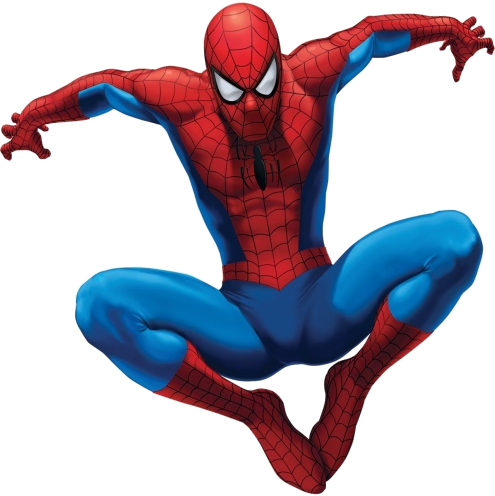
\includegraphics[height=2.9cm]{les2-hero-1}};
  \node[anchor=north] (hero2) at (0.8,2.05)
  {
\includegraphics[height=4cm]{les2-hero-2}};
  \node[anchor=north] (hero3) at (1.3,1.575)
  {
\includegraphics[height=3.1cm]{les2-hero-3}};
  \node[anchor=north] (hero4) at (1.8,2.1)
  {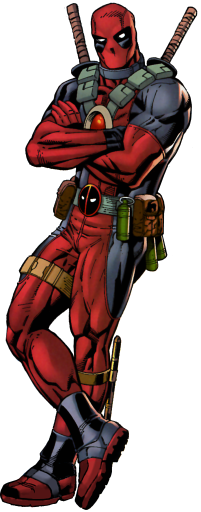
\includegraphics[height=4.1cm]{les2-hero-4}};
  \node[anchor=north] (hero5) at (2.3,1.95)
  {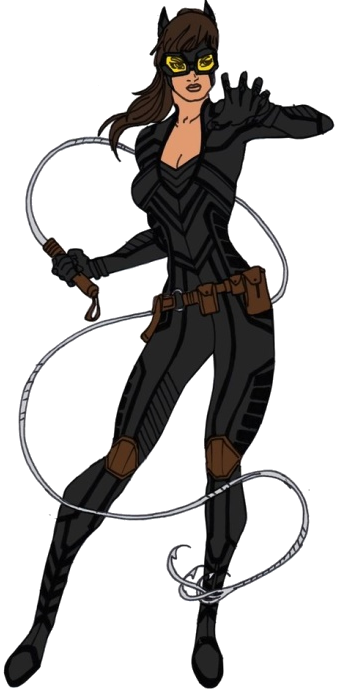
\includegraphics[height=3.8cm]{les2-hero-5}};
  
  \node (size1) at (0.3, 1.5) {\scriptsize 141 cm};
  \node (size2) at (0.8, 2.1) {\scriptsize 198 cm};
  \node (size3) at (1.3, 1.51) {\scriptsize 143 cm};
  \node (size4) at (1.8, 2.15) {\scriptsize 201 cm};
  \node (size5) at (2.3, 1.95) {\scriptsize 184 cm};
  \end{tikzpicture}
  \caption{De lengte van enkele superhelden.}
  \label{fig:helden}
\end{figure}

\subsection{Gemiddelde}
\label{sec:gemiddelde}

\begin{definition}[Gemiddelde]
  \index{Gemiddelde} Het rekenkundig gemiddelde (symbool $\overline{x}$, Eng. \index{mean}\emph{mean}, \index{average}\emph{average}) van een verzameling waarden is de som van al deze waarden gedeeld door het aantal waarden.
  \begin{equation}
    \overline{x} = \frac{1}{n} \sum_{i=1}^{n} x_{i}
    \label{eq:Mean}
  \end{equation}

  Waarbij:
  \begin{itemize}
    \item $x_{i}$ de verschillende waarden zijn (in het voorbeeld van Figuur~\ref{fig:helden} zijn dit 141, 198, 143, enz.)
    \item $n$ het aantal waarden is (in het voorbeeld is $n = 5$).
  \end{itemize}
\end{definition}

\begin{remark}[!!]
  Merk op dat we met het symbool $\overline{x}$ specifiek het gemiddelde van een \emph{steekproef} aanduiden. Het gemiddelde van een \emph{populatie} wordt aangeduid met de Griekse letter mu, $\mu$.
  
  Zie Appendix~\ref{app:notatie} voor een overzicht van de gebruikte symbolen en notaties in deze cursus.
\end{remark}

\begin{exercise}
  Wat is de gemiddelde lengte van de superhelden?
\end{exercise}

\begin{exercise}
  Vraag: het gemiddelde van 15 cijfers is 12. Welk nummer moeten
  we aan de rij van cijfers toevoegen om een gemiddelde van 13 te bekomen?
\end{exercise}

\begin{exercise}
  Men zegt dat het rekenkundig gemiddelde gevoelig is aan uitschieters: een extreme waarde kan het rekenkundig gemiddelde zwaar beïnvloeden. 
  
  Stel je voor dat Kabouter Wesley (10 cm) toegevoegd wordt aan het team superhelden. Wat wordt dan de gemiddelde lengte?
\end{exercise}

\subsection{Variantie en standaardafwijking}
\label{sec:varEnSD}

De spreidingsmaat die typisch geassocieerd wordt met het gemiddelde is de standaardafwijking. Voordat we die definiëren, geven we eerst die van de \emph{variantie}.

\begin{definition}[Variantie]
  De \index{variantie} variantie van een steekproef (symbool $s^{2}$, Eng. \index{variance}\emph{sample variance}) is de som van de gekwadrateerde verschillen tussen de waarde van de dataset en het gemiddelde, gedeeld door het aantal waarden min één:
  \begin{equation}
  s^{2} = \frac{1}{n-1} \sum_{i=1}^{n} \left(\overline{x} - x_i \right)^{2}
  \label{eq:variantie}
  \end{equation}
\end{definition}

Het is je misschien opgevallen dat in de formule gedeeld wordt door $n-1$ en niet door $n$, wat je zou kunnen verwachten. Er bestaat ook effectief een variant van de formule met $n$ in de noemer. Dit noemen we de populatievariantie, aangeduid met $\sigma^2$ (de Griekse letter sigma).

De variantie van een steekproef wordt in de praktijk gebruikt als een schatting voor de (onbekende) populatievariantie. De formule met $n-1$ in de noemer is een zgn.~\textit{zuivere schatter} is, wat betekent dat bij veel herhalingen het gemiddelde van de schattingen convergeert naar de te schatten populatievariantie. Je kan dit wiskundig bewijzen, maar dat valt buiten het bestek van deze cursus.

\begin{example}
  De variantie bij de lengtes van onze superhelden wordt als volgt berekend:
  
  \begin{align*}
  	s^{2} & =  \frac{(173,4 - 141)^{2} + (173,4 - 198 )^{2} + (173,4 - 143)^{2} + (173,4 - 201)^{2} + (173,4 - 184 )^{2}}{4} \\
  	      & =  \frac{(-32,4)^{2} + (24,6)^{2} + (-30,4)^{2} + (27,6)^{2} + (10,6)^{2}}{4}                                    \\
  	      & = \frac{1049,76 + 605,16 + 924,16 + 761,76 + 112,36}{4}                                                          \\
  	      & = \frac{3453,2}{4} = 863,3
  \end{align*}
\end{example}

Bij de berekening van de steekproefvariantie wordt er gedeeld door $n-1$ en niet door $n$. Waarom? Aangezien de som van de afwijkingen $x_{i} - \overline{x}$ steeds 0 oplevert (zie hieronder in vergelijking \ref{eq:sumGemid}), kan de laatste afwijking gevonden worden uit de eerste $n-1$ afwijkingen. We berekenen dus niet het gemiddelde van $n$ getallen zonder verwantschap. Slecht $n-1$ van de gekwadrateerde afwijkingen kunnen vrij bewegen, daarom berekenen we het gemiddelde door het totaal te delen door $n-1$. Het getal $n-1$ noemt men het aantal \index{vrijheidsgraden}\emph{vrijheidsgraden} van de variantie.

\begin{equation}
 \sum_{i}^{n}(x_{i} - \overline{x}) = \sum_{i}^{n}x_{i} - \sum_{i}^{n}\overline{x} = \sum_{i}^{n}x_{i} - n \left(\frac{1}{n}\sum_{i}^{n} x_{i}\right)
\label{eq:sumGemid}
\end{equation}

\begin{definition}[Standaardafwijking]
  De \index{standaardafwijking} standaardafwijking (Eng. \index{standard deviation}\emph{standard deviation}) wordt dan gedefinieerd als de vierkantswortel van de variantie.
  \begin{equation}
  s = \sqrt{s^{2}} = \sqrt{\frac{1}{n-1} \sum_{i=1}^{n} \left(\overline{x} - x_i \right)^{2}}
  \label{eq:stdev}
  \end{equation}
\end{definition}

\begin{remark}[!!]
  Ook hier hebben we specifiek de variantie en standaardafwijking van een \emph{steekproef} gedefinieerd. De standaardafwijking van een \emph{populatie} wordt aangeduid met de Griekse letter sigma, $\sigma$.
\end{remark}

Dit geeft ons dus inzicht in wat normaal is en wat abnormaal is: een kleine standaardafwijking wijst erop dat de waarden dicht bij de centrummaat ($\overline{x}$) liggen, terwijl een grote standaardafwijking aangeeft dat de waarden verder verspreid liggen. In sommige gevallen wil men een grote standaardafwijking, in andere gevallen niet zoals hieronder beschreven.

\begin{example}
  Bij het vervaardigen van een schroevendraaier is de grootte van de kop belangrijk voor het goed functioneren van de schroevendraaier. Als we dus van 100 verschillende schroevendraaiers de kopgrootte meten, is het beter dat die grootte redelijk constant is en wensen we dus een kleine standaardafwijking.
\end{example}

\begin{example}
  Bij het onderzoek naar onze superhelden, wensen we te weten hoeveel ze ongeveer verdienen in hun normale job. We hebben een aantal rijke superhelden (bv. Batman) en een aantal minder rijke superhelden (bv. Spiderman). De spreiding op hun inkomen is dus groot, maar dat is niet per definitie een probleem.
\end{example}

Een aangename eigenschap van de standaardafwijking is dat het uitgedrukt kan worden in dezelfde metriek als de gemeten data. Bij ons voorbeeld van de superhelden, wil dat zeggen dat de standaardafwijking (ongeveer) 29,38 cm is.

Zoals het gemiddelde zijn de variantie en de standaarddeviatie gevoelig aan uitschieters. De variantie is eigenlijk gevoeliger dan het gemiddelde. Inderdaad, voor een uitschieter is de afstand tot het gemiddelde kleiner dan het kwadraat van deze afstand. % TODO: Wat wordt hiermee bedoeld?

\subsection{Mediaan}

De mediaan is een alternatieve centrummaat die als voordeel ten opzichte van het gemiddelde heeft dat die een stuk minder gevoelig is voor uitschieters.

\begin{definition}[Mediaan]
  Indien we alle metingen sorteren van klein naar groot, is de \index{mediaan} mediaan (Eng. \index{median}\emph{median}) het middelste cijfer. Als het aantal cijfers even is, neemt men het gemiddelde van de twee middelste cijfers.
\end{definition}

\begin{exercise}
  Wat is de mediaan van de lengtes van de superhelden?
\end{exercise}

\begin{exercise}
  Wat wordt de mediaan als Kabouter Wesley er bij komt? Is de impact groter of kleiner dan bij het gemiddelde?
\end{exercise}

\subsection{Bereik}

\begin{definition}[Bereik]
  Het \index{bereik}bereik (Eng. \index{range}\emph{range}) van een variabele is de absolute waarde van het verschil tussen de grootste en kleinste waarde.
  \begin{equation}
    | max_i(x_i) - min_i(x_i) |
  \end{equation}
\end{definition}

Het bereik van een variabele is vaak niet zo interessant als spreidingsmaat omdat ze zeer gevoelig is voor uitschieters.

\subsection{Kwartielen \& kwartielafstand}

De interkwartielafstand is een betere spreidingsmaat die veel minder gevoelig is voor uitschieters. Om te begrijpen hoe ze werkt, moeten we eerst het begrip \emph{kwartielen} definiëren.

\begin{definition}[Kwartielen]
  De \index{kwartiel} kwartielen zijn de waarden die een gesorteerde lijst van waarden in 4 gelijke delen deelt. Elk deel vormt dus een kwart van de dataset. Men spreekt van een eerste, tweede en derde kwartiel ($Q_{1}$, $Q_{2}$, $Q_{3}$).
\end{definition}

Dus:

\begin{itemize}
  \item het eerste kwartiel $Q_{1}$ is de waarde die de laagste 25 \% van de reeks afscheidt.
  \item het tweede kwartiel $Q_{2}$ is de waarde die de laagste 50\% van de reeks afscheidt.
  \item het derde kwartiel $Q_{3}$ is de waarde die de laagste 75\% van de reeks afscheidt.
\end{itemize}

Om te bepalen welke waarden in een gesorteerde rij precies de kwartielen zijn, ga je als volgt te werk (volgens \textcite{Moore2002}):

Als $n$ oneven is:

\begin{itemize}
  \item $Q_{1}$ is het $\frac{n+1}{4}$e getal
  \item $Q_{3}$ is het $\frac{3n+3}{4}$e getal
\end{itemize}

Als $n$ even is:

\begin{itemize}
  \item $Q_{1}$ is het $\frac{n+2}{4}$e getal
  \item $Q_{3}$ is het $\frac{3n+2}{4}$e getal
\end{itemize}

\begin{exercise}
  Met welke hiervoor gedefinieerde statistiek komt $Q_{2}$ overeen?
\end{exercise}

\begin{definition}[Interkwartielafstand]
  De \index{interkwartielafstand}interkwartielafstand (Eng. \index{interquartile range}InterQuartile Range, $IQR$) is het verschil tussen het derde en eerste kwartiel.
  
  \begin{equation}
    IQR = Q_3 - Q_1
  \end{equation}
\end{definition}

De definitie van kwartielen kan worden veralgemeend naar \index{deciel}\emph{decielen} (waarden die de dataset in tien gelijke delen verdelen) en \index{percentiel}\emph{percentielen} (honderd gelijke delen). Het 65e percentiel, bijvoorbeeld is dan het getal in de gesorteerde rij waarvoor geldt dat 65\% van de waarden \emph{kleiner} is dan dat getal.

\section{Visualisatie van één variabele}

Ook bij het visualiseren van één variabele hangt het meest geschikte grafiektype af van het meetniveau. In Tabel~\ref{tab:grafiektypes-1-variabele} vind je een overzicht.

\begin{table}
  \centering
  \begin{tabular}{ll}
  	\toprule
  	\textbf{Meetniveau} & \textbf{Grafiektype}          \\
  	\midrule
  	Kwalitatief         & Staafdiagram van frequenties  \\
  	\midrule
  	Kwantitatief        & Boxplot, histogram, dichtheid \\
  	\bottomrule
  \end{tabular}
  \caption{Geschikte grafiektypes per meetniveau voor het visualiseren van één variabele.}
  \label{tab:grafiektypes-1-variabele}
\end{table}

\subsection{Staafdiagram}

Bij het visualiseren van een kwalitatieve variabele wordt eerst een frequentietabel opgesteld van alle voorkomende waarden.

\begin{definition}[Frequentietabel]
  Een \index{frequentietabel}\emph{frequentietabel} is tabel waarin opgesomd staat hoeveel keer een waarde voorkomt in de volledige dataset (= frequentie). Meestal zijn de tabellen verticaal georiënteerd.
\end{definition}

Om de een \index{staafdiagram}\emph{staafdiagram} (zie Figuur~\ref{fig:staafdiagram}) te tekenen worden de verschillende waarden opgesomd onder de X-as en voor elke waarde wordt een staaf getekend waarvan de hoogte bepaald wordt door het aantal keer dat de overeenkomstige waarde voorkomt.

\begin{figure}
  \centering
  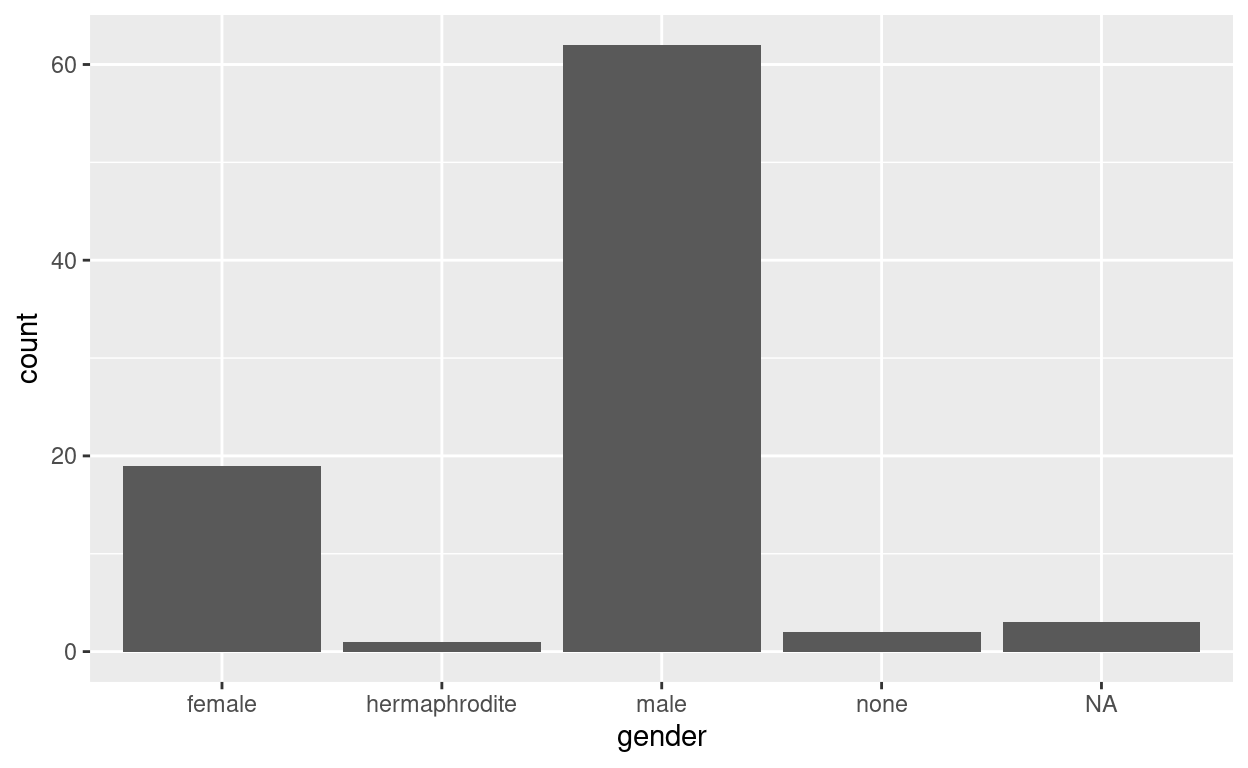
\includegraphics[width=.7\textwidth]{staafdiagram}
  \caption[Voorbeeld van een staafdiagram]{\textbf{Voorbeeld van een staafdiagram.} De labels op de x-as duiden de mogelijke waarden van de gevisualiseerde kwalitatieve variabele aan. De hoogte van elke staaf geeft de frequentie aan van elke waarde binnen de steekproef.}
  \label{fig:staafdiagram}
\end{figure}

\subsection{Boxplot}

De \index{boxplot}\emph{boxplot} (zie Figuur~\ref{fig:boxplot}) wordt gevormd door een rechthoek begrensd door de kwartielwaarden (25\% en 75\%). In deze rechthoek wordt ook de mediaan getekend. De stelen, die aan de rechthoek zitten, bevatten de rest van de waarnemingen, op de uitschieters en extremen na.

\begin{itemize}
  \item Een \index{uitschieter}\textit{uitschieter} is een waarde die meer dan 1,5 keer de interkwartielafstand boven/onder het derde/eerste kwartiel ligt en wordt aangeduid met een cirkeltje.
  \item Een \index{extremum}\textit{extremum} is een waarde die meer dan 3 keer de interkwartielafstand boven/onder het derde/eerste kwartiel ligt en wordt in een boxplot aangeduid met een sterretje.
\end{itemize}

Een boxplot wordt horizontaal of verticaal georiënteerd, op basis van wat het duidelijkst is.

\begin{figure}
  \centering
  % Source: http://mirrors.ibiblio.org/CTAN/graphics/pgf/contrib/pgfplots/doc/pgfplots.pdf
  % p.430
  \begin{tikzpicture}
    \begin{axis}[x=3cm,xticklabels={},xmax=2.3]
      \addplot+[
      boxplot prepared={
        draw direction=y,
        lower whisker=5,
        lower quartile=7,
        median=8.5,
        upper quartile=9.5,
        upper whisker=10,
      },
      ]
      table[row sep=\\,y index=0] {
        data\\ 1\\ 3\\
      }
      [right,color=hgorange]
      node at (boxplot box cs: 1,.6) {uitschieter}
      node at (boxplot box cs: \boxplotvalue{lower quartile},1) {$Q_1$}
      node at (boxplot box cs: \boxplotvalue{median},1)         {$Q_2$, mediaan}
      node at (boxplot box cs: \boxplotvalue{upper quartile},1) {$Q_3$}
      node at (boxplot box cs: \boxplotvalue{upper whisker},1)  {max}
      ;
    \end{axis}
  \end{tikzpicture}
  \caption[Voorbeeld van een boxplot]{\textbf{Voorbeeld van een boxplot.} De blauwe rechthoek duidt het interval aan waarbinnen de helft van de waarnemingen zich bevinden. De grenzen zijn het eerste kwartiel onderaan ($Q_1$) en het derde bovenaan ($Q_3$). De lijn in het midden van de rechthoek is de mediaan (of het tweede kwartiel, $Q_2$). De andere blauwe horizontale strepen duiden in principe de kleinste en grootste waarnemingen aan. In dit geval zijn er echter enkele waarnemingen die erg ver van de mediaan liggen. Deze worden uitschieters genoemd en worden apart geplot als een punt.}
  \label{fig:boxplot}
\end{figure}

\subsection{Histogram}

Een \index{histogram}\emph{histogram} (zie Figuur~\ref{fig:histogram}) is een soort staafdiagram, maar dan aangepast naar kwantitatieve variabelen. Het bereik van de variabele wordt onderverdeeld in een door de onderzoeker gekozen aantal, typisch even grote, intervallen of klassen. Voor elke klasse wordt er geteld hoeveel waarnemingen er binnen vallen en op basis daarvan wordt de hoogte van de staven bepaald.

\begin{figure}
  \centering
  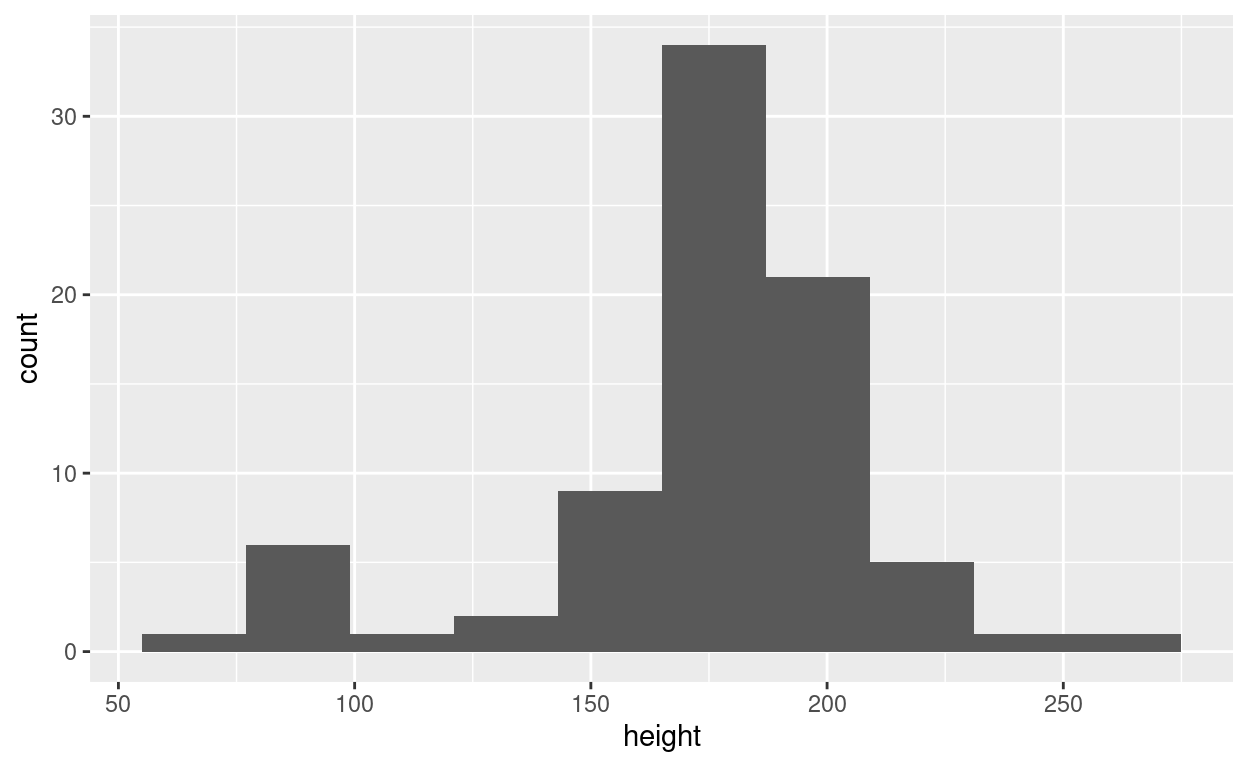
\includegraphics[width=.7\textwidth]{histogram}
  \caption[Voorbeeld van een histogram]{\textbf{Voorbeeld van een histogram.} De X-as is hier onderverdeeld in een aantal even grote intervallen. De hoogte van elke staaf is gebaseerd op het aantal waarnemingen binnen elk interval.}
  \label{fig:histogram}
\end{figure}

\subsection{Dichtheidsgrafiek}

De duidelijkheid van een histogram hangt in grote mate af van de keuze van de intervallen. Als deze te groot gekozen zijn verlies je precisie, en als ze te klein zijn zullen verschillende intervallen geen observaties bevatten. Als alternatief voor een histogram kan je ook een \index{dichtheidsgrafiek}\index{kansdichtheidsgrafiek}(kans)dichtheidsgrafiek (zie Figuur~\ref{fig:dichtheidsgrafiek}) plotten. De X-as is dan niet onderverdeeld in klassen. Er wordt een continue curve getekend waarvan de hoogte overeenkomt met de hoeveelheid waarnemingen ``in de buurt''. Een dichtheidsgrafiek toont typisch nog beter hoe de waarnemingen gespreid zijn.

\begin{figure}
  \centering
  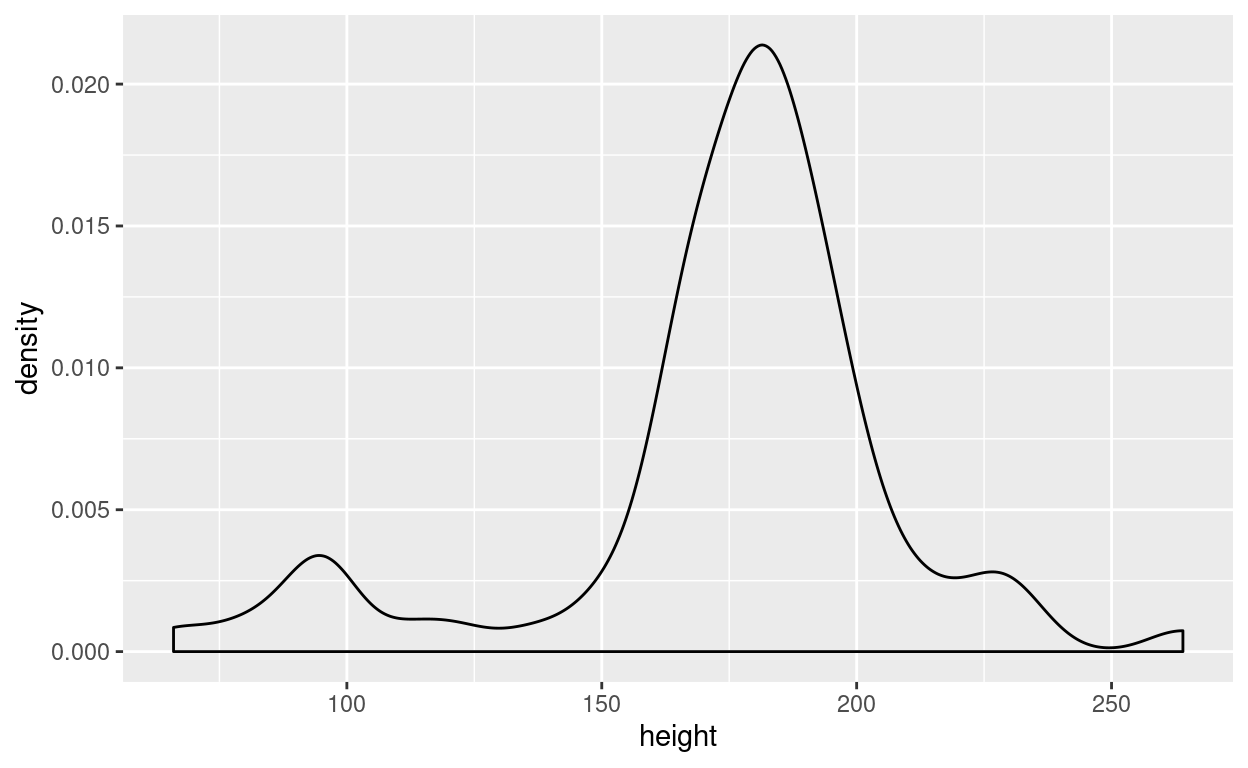
\includegraphics[width=.7\textwidth]{dichtheidsgrafiek}
  \caption[Voorbeeld van een dichtheidsgrafiek]{\textbf{Voorbeeld van een (kans)dichtheidsgrafiek.} De grafiek toont dezelfde data als het histogram in Figuur~\ref{fig:histogram}.}
  \label{fig:dichtheidsgrafiek}
\end{figure}





% Exercises
\section{Oefeningen}

\subsection{Centrum- en spreidingsmaten}

\begin{exercise}
  \label{ex:mean-stdev-freq}
  De formules voor het steekproefgemiddelde $\overline{x}$, de steekproefvariantie $s^2$ en de standaarddeviatie $s$ staan beschreven in secties \ref{sec:gemiddelde} en \ref{sec:varEnSD}.
  Hoe moeten deze formules aangepast worden om $\overline{x}$, $s^2$ en $s$ te berekenen wanneer we te maken hebben met een frequentietabel? 
  Doe dit voor de data in Tabel~\ref{tab:pinfreq}.
\end{exercise}

\begin{table}
  \centering
  \begin{tabular}{cc}
  	\toprule
  	Pinnen $x$ & Frequentie $f_{x}$ \\
  	\midrule
  	    0      &         2          \\
  	    1      &         1          \\
  	    2      &         2          \\
  	    3      &         0          \\
  	    4      &         2          \\
  	    5      &         4          \\
  	    6      &         9          \\
  	    7      &         11         \\
  	    8      &         13         \\
  	    9      &         8          \\
  	    10     &         8          \\
  	\bottomrule
  \end{tabular}
  \caption{Tijdens het spelen van een kegelspel is bijgehouden hoeveel pinnen telkens omver gegooid werden. Voor elke mogelijke score $x$ is bijgehouden hoeveel keer.}
  \label{tab:pinfreq}
\end{table}

\begin{exercise}
  \label{ex:variance-formula}
  In de formule voor de steekproefvariantie wordt het verschil tussen de meetpunten en het gemiddelde gekwadrateerd. Waarom? Zouden we geen eenvoudiger formule kunnen bedenken die een even goede maatstaf is voor de spreiding van een dataset? Hieronder vind je drie voorstellen (de derde is de ``echte'' formule).

  \begin{align}
    s^{2}_{1} &= \frac{1}{n-1} \sum_{i=1}^{n} (\overline{x} - x) \\
    s^{2}_{2} &= \frac{1}{n-1} \sum_{i=1}^{n} \left| \overline{x} - x\right| \\
    s^{2}_{3} &= \frac{1}{n-1} \sum_{i=1}^{n} (\overline{x} - x)^{2}
  \end{align}

  Pas elke formule toe op de twee datasets hieronder. Door het resultaat te vergelijken zou je moeten kunnen besluiten of de formules geschikt zijn als een spreidingsmaat.
  
  \begin{align*}
    X &= \left\{ 4,4,-4,-4 \right\} \\
    Y &= \left\{ 7,1,-6,-2 \right\}
  \end{align*}

\end{exercise}

\begin{exercise}
  Zoek eens zelfstandig op wat de variatieco\"effici\"ent voor een steekproef is. Hoe wordt die gedefinieerd voor een volledige populatie en wat zou je ermee kunnen doen?
\end{exercise}

\begin{exercise}
  \label{ex:ais}
  Importeer het bestand \texttt{ais.csv} in R (terug te vinden in de Github-repository van deze cursus, in de map \texttt{oefeningen/datasets}). 
  Een beschrijving van dit data frame is terug te vinden in dezelfde map, bestand \texttt{ais.html}.
  
  Je kan dit bestand importeren met behulp van volgende code:
  \begin{lstlisting}
  ais <- read.csv("ais.csv", sep = ",")
  attach(ais)
  \end{lstlisting}
  
  Beschouw de volgende deelverzamelingen uit dit data frame, 
  en bereken voor elk de geschikte centrum- en spreidingsmaten van de variabelen \texttt{sex} en \texttt{ht}.
  
  \begin{enumerate}
    \item de roeiers.
    \item de roeiers, de netballers en de tennissers samen.
    \item de vrouwelijke basketballers en roeiers.
  \end{enumerate}
\end{exercise}

\begin{exercise}
  \label{ex:mean-range-R}
  Gebruik de functies \texttt{mean} en \texttt{range} in R om het gemiddelde en bereik te bepalen van:
  \begin{itemize}
    \item de cijfers 1, 2, \dots, 21.
    \item 50 willekeurige normale waarden, die  worden gegenereerd vanuit een normale distributie met gemiddelde 0 en variantie 1 (functie \texttt{rnorm}).
    \item de kolommen \texttt{height} en \texttt{weight} in de data frame \texttt{women} (standaard in R).
  \end{itemize}
\end{exercise}

In vorige oefeningen hebben we de verschillende spreidingsmaten en centrummaten besproken. Zoals je merkt worden deze metrieken ook gebruikt in het onderzoek van~\textcite{Akin2016}. In de volgende oefeningen gaan we trachten de resultaten te reproduceren.

Hiervoor hebben we het bestand \texttt{android\_persistence\_cpu.csv} nodig. Je vindt deze eveneens terug in de folder \texttt{oefeningen/datasets}.

\begin{exercise}
  \label{oef:casus-akin2016-1var}
	Open de file met excel en bekijk de structuur van het document. Hoe ziet die er uit? Kan je de variabelen identificeren en hun type benoemen. 
\end{exercise}

We gaan het programma \texttt{R} gebruiken samen met \texttt{RStudio}. Open de file in \texttt{RStudio}.

\begin{lstlisting}[breaklines=true]
  android_cpu <- read.csv("android_persistence_cpu.csv", sep=";", dec=",")
  attach(android_cpu)
\end{lstlisting}

We hebben nu de data ingeladen. We kunnen eens kijken wat de gemiddelde tijd, de standaarddeviatie, de kwartielen e.a. zijn. Gebruik hiervoor de commando's \texttt{mean}, \texttt{median}, \texttt{quantile}, \texttt{min}, \texttt{max}, \texttt{var}, \texttt{sd}. Je kan ook makkelijk gebruik maken van de methode \texttt{summary}.

\begin{exercise}
	Als je de vorige metrieken berekend hebt, wat kan je daar dan over zeggen. Kan je zinnige conclusies trekken uit de vorige resultaten. Zo ja vermeld ze, zo nee beschrijf waarom je dat denkt.
\end{exercise}

% TODO: Oefening over percentielen toevoegen, bv. gebaseerd op 95th percentile bandwith metering
% https://www.semaphore.com/95th-percentile-bandwidth-metering-explained-and-analyzed/
% http://aboutcolocation.info/95th-percentile-monitoring-explained/

\subsection{Grafieken in R}

% TODO: verwijderen uit de cursus, verplaatsen naar labos

Een histogram is een eenvoudige plot. Het toont de frequenties van de data die in een bepaald bereik voorkomen. 

\begin{lstlisting}[breaklines=true]
  hist(android_cpu$Time, main="Distribution of execution time", xlab="Execution time (ms)")
  hist(android_cpu$Time, main="Distribution of execution time", xlab="Execution time (ms)", breaks=2)
\end{lstlisting}
\begin{exercise}
	Wat concludeer je als je bovenstaande grafiek\footnote{Heb je wat problemen met het genereren van grafieken, volgende link \url{https://www.datacamp.com/community/tutorials/15-questions-about-r-plots\#gs.RK_ORsI} bevat een aantal goede tips and tricks om je op weg te helpen.} genereert? Is dit een zinnig resultaat? Wat gebeurt er als je de variabele breaks verhoogt?
\end{exercise}

Een boxplot toont de mediaan, de kwartielen, het maximum en het minimum van een dataset. Dit geeft ons een duidelijk impressie van hoe de data er uitziet.

\begin{lstlisting}[breaklines=true]
boxplot(android_cpu$Time)
boxplot(android_cpu$Time, main='Distribution of execution time', ylab="Execution time (ms)")
\end{lstlisting} 

\begin{exercise}
	De boxplot wordt standaard verticaal getekend. Gebruik het commando \texttt{help(boxplot)} om uit te zoeken hoe we de tekening horizontaal krijgen. 
\end{exercise}

Als je goed geantwoord hebt op de volgende vragen merk je natuurlijk dat het weinig zin heeft de volledige dataset te analyseren, aangezien de dataset verdeeld is over verschillende categorie\"en. We willen dus wel deze statistieken weten, maar per categorie. We kunnen dus een boxplot maken voor elke categorie.

\begin{lstlisting}[breaklines=true]
boxplot(android_cpu$Time ~ android_cpu$DataSize, main="Distribution of CPU time over the data sizes", ylab="Time in ms");
\end{lstlisting}

\begin{exercise}
	\label{ex:boxplot}
	Interpreteer de resultaten die je behaalt uit deze grafiek. Zijn deze al wat zinniger?
\end{exercise}

We kunnen hetzelfde doen voor de verschillende soorten dataopslagmogelijkheden in android.

\begin{exercise}
	Zelfde vraag als \ref{ex:boxplot}. Interpreteer de resultaten die je behaalt uit deze grafiek. Zijn deze al wat zinniger?
\end{exercise}

We kunnen eens kijken hoe de data eruit ziet over alle categorie\"en heen.

\begin{lstlisting}[breaklines=true]
  boxplot(android_cpu$Time ~ android_cpu$PersistenceType * android_cpu$DataSize, main="Distribution of CPU time over data sizes for the different persistent types", ylab="Time in ms");
\end{lstlisting}

Het blijkt dat we wel al een duidelijker zicht krijgen over de data over de categorie\"en heen, maar de figuur is op dit moment te druk. 

We moeten de data dus onderverdelen in categorie\"en namelijk onder \texttt{PersistentieType} en \texttt{Datahoeveelheid}. We gaan hiervoor de functie \texttt{which}\footnote{Je kan ook gebruik maken van de functie \texttt{subset}, wat misschien zelfs eenvoudiger is} gebruiken en kijken hoe de verschillende datahoeveelheden verschillen per datahoeveelheidcategorie. 

\begin{lstlisting}[breaklines=true]
  greenDOA <- android_cpu[which(android_cpu$PersistenceType=='GreenDAO'),];
  boxplot(greenDOA$Time ~ greenDOA$DataSize);
\end{lstlisting}

\begin{exercise}
  Wat concludeer je uit de vorige grafiek?
\end{exercise}

\begin{exercise}
  Ga nu zelf na welke boxplots er interessant zijn om te maken, en kijken of jouw resultaten overeen met die van \textcite{Akin2016}. Welke conclusies trek je?
\end{exercise}

\begin{exercise}[Retrieval practice]
  Gebruik de procedure voor retrieval practice uit oefening~\ref{ex:retrieval-practice-meetniveaus} om de \emph{analyse- en visualisatietechnieken voor één variabele} in te studeren.
  
  Geef per meetniveau:
  
  \begin{itemize}
    \item De geschikte centrum- en spreidingsmaten (naam + definities en evt.~formules)
    \item Geschikte grafiektypes
  \end{itemize}
\end{exercise}





% Answers
\subsection{Antwoorden op geselecteerde oefeningen}

\paragraph{Oefening \ref{ex:mean-stdev-freq}}

\begin{itemize}
  \item $\overline{x} = 7$
  \item $s^2 \approx 5.830508$
  \item $s \approx 2.414645$
\end{itemize}

\paragraph{Oefening \ref{ex:variance-formula}}
Tabel \ref{tab:opl-variance-ht} geeft een overzicht van de aangepaste steekproefvariantie voor beide datasets.

\begin{table}
  \centering
  \begin{tabular}{@{}l|rrr@{}}
    \toprule
      & \textbf{$s^{2}_{1}$} & \textbf{$s^{2}_{2}$} & \textbf{$s^{2}_{3}$} \\
    \midrule                
      \textbf{$ X $} & 0           & 5.333333    & 21.33333    \\ 
      \textbf{$ Y $} & 0           & 5.333333    & 30          \\           
    \bottomrule
  \end{tabular}
  \caption{Resultaten van de aangepaste steekproefvariantie voor beide datasets, voor de verschillende formules van oefening \ref{ex:variance-formula}.}
  \label{tab:opl-variance-ht}
\end{table}

\paragraph{Oefening \ref{ex:ais}}

Tabel \ref{tab:opl-ais-ht} geeft een overzicht met de belangrijkste centrum- en spreidingsmaten voor de variabele \texttt{ht} (height, lengte) over de gevraagde groepen.

\begin{table}
  \centering
  \begin{tabular}{@{}l|r|rrrr|rr@{}}
    \toprule
    & \textbf{(1)} & \multicolumn{4}{c}{\textbf{(2)}}                                                 & \multicolumn{2}{c}{\textbf{(3)}} \\ 
    & \textbf{Row} & \textbf{Total}    & \textbf{Row} & \textbf{Netball} & \textbf{Tennis} & \textbf{B\_ball}  & \textbf{Row} \\ \midrule
    \textbf{gemiddelde} & 182.376      & 179.066                      & 182.376      & 176.087          & 174.164         & 182.269           & 178.859      \\
    \textbf{stdev}      & 7.798        & 7.936                        & 7.798        & 4.124            & 9.858           & 8.621             & 5.970        \\
    \textbf{min}        & 156.000      & 156.000                      & 156.000      & 168.600          & 157.900         & 169.100           & 156.000      \\
    \textbf{Q1}         & 179.300      & 174.200                      & 179.300      & 173.450          & 167.300         & 174.000           & 177.600      \\
    \textbf{mediaan}    & 181.800      & 179.500                      & 181.800      & 176.000          & 175.000         & 184.600           & 179.650      \\
    \textbf{Q3}         & 186.300      & 183.400                      & 186.300      & 179.150          & 180.750         & 188.700           & 181.200      \\
    \textbf{max}        & 198.000      & 198.000                      & 198.000      & 183.300          & 190.800         & 195.900           & 186.300      \\
    \textbf{IQR}        & 7.000        & 9.150                        & 7.000        & 5.700            & 13.450          & 14.700            & 3.600        \\ \bottomrule
  \end{tabular}
  \caption{Overzicht resultaten in oefening \ref{ex:ais} voor de variabele \texttt{ht} (height/lengte), met drie cijfers na de komma. In deeloefening 2 zijn de resultaten zowel gegeven voor de hele groep (roeiers, netballers én tennissers) als opgesplitst (via de functie \texttt{aggregate}).}
  \label{tab:opl-ais-ht}
\end{table}

In deeloefening 1 en 2 nemen we de variabele \texttt{sex} als voorbeeld. Zie tabel \ref{tab:opl-ais-sex} voor een overzicht. Over kwalitatieve variabelen valt minder te zeggen, we geven hier een frequentietabel waaruit we de modus kunnen afleiden.

In deeloefening 3 zijn enkel vrouwen geselecteerd, en voor deze oefening tonen we in tabel \ref{tab:opl-ais-sport} de frequenties van variabele \texttt{sport}.

\begin{table}
  \centering
  \begin{tabular}{@{}l|r|rrrr}
  	\toprule
  	               & \textbf{(1)} &                    \multicolumn{4}{c}{\textbf{(2)}}                     \\
  	               & \textbf{Row} & \textbf{hele groep} & \textbf{Row} & \textbf{Netball} & \textbf{Tennis} \\ \midrule
  	\textbf{f}     &           22 &                  52 &           22 &               23 &               7 \\
  	\textbf{m}     &           15 &                  19 &           15 &                0 &               4 \\
  	\textbf{modus} &            f &                   f &            f &                f &               f \\ \bottomrule
  \end{tabular}
  \caption{Overzicht resultaten in oefening \ref{ex:ais} (1) en (2) voor de variabele \texttt{sex}. Meer bepaald zijn hier de frequenties van de waarden opgegeven, en ook telkens de modus.}
  \label{tab:opl-ais-sex}
\end{table}

\begin{table}
  \centering
  \begin{tabular}{@{}l|l}
  	\toprule
  	                 & Frequenties \\ \midrule
  	\textbf{B\_ball} & 13          \\
  	\textbf{Row}     & 22          \\
  	\textbf{modus}   & Row         \\ \bottomrule
  \end{tabular}
  \caption{Overzicht resultaten in oefening \ref{ex:ais} (3) voor de variabele \texttt{sport}.}
  \label{tab:opl-ais-sport}
\end{table}


\paragraph{Oefening \ref{ex:mean-range-R}}
Tabel~\ref{tab:opl-mean-range-R} geeft een overzicht van het gemiddelde en bereik voor oefening~\ref{ex:mean-range-R}.

\begin{table}
  \centering
  \begin{tabular}{@{}l|r|rl@{}}
    \toprule
      & \textbf{Gemiddelde} & \multicolumn{2}{c}{\textbf{Bereik}} \\
    \midrule                
                  \textbf{$1,2,...,21$} & 11       & 1    & 21    \\ 
        \textbf{\texttt{women\$height}} & 65       & 58   & 72    \\
        \textbf{\texttt{women\$weight}} & 136.7333 & 115  & 164   \\
    \bottomrule
  \end{tabular}
  \caption{Gemiddele en bereik voor de datasets van oefening \ref{ex:mean-range-R}.}
  \label{tab:opl-mean-range-R}
\end{table}

\chapter{De centrale limietstelling}
\label{ch:centrale-limietstelling}

In dit hoofdstuk wordt de Centrale Limietstelling geïntroduceerd (zie Sectie~\ref{sec:centrale-limietstelling}). Dit is voor het vakgebied van de statistiek een enorm belangrijk resultaat omdat de gehele theorie van statistische toetsen (zie Hoofdstuk~\ref{ch:toetsingsprocedures}) hierop gebaseerd is. De Centrale Limietstelling laat toe om metingen op basis van een steekproef onder bepaalde voorwaarden te veralgemenen naar de populatie als geheel.

We bespreken eveneens het concept van puntschatters en betrouwbaarheidsintervallen. Een puntschatter is een getal dat berekend wordt uit de steekproef, waarmee men een schatting wil maken van een eigenschap van de populatie. Het steekproefgemiddelde $\overline{x}$ is bijvoorbeeld een puntschatter voor het populatiegemiddelde $\mu$. Een betrouwbaarheidsinterval drukt uit tussen welke grenzen men vermoed dat een bepaalde waarde zich bevindt, en hoe zeker men hiervan is. Een 95\%-betrouwbaarheidsinterval voor het populatiegemiddelde, bijvoorbeeld, is een interval dat opnieuw berekend is aan de hand van de steekproef, waarvan we--onder duidelijke voorwaarden--met 95\% zekerheid kunnen zeggen dat het populatiegemiddelde er in zal liggen.

Voordat we deze begrippen kunnen introduceren, is het nodig eerst enkele begrippen uit de kansrekening te herhalen (zie Sectie~\ref{sec:kansverdeling-steekproef}) en de normale verdeling  (zie Sectie~\ref{sec:normale-verdeling}) te bespreken.

\section{Leerdoelen}
\label{sec:centrale-limietstelling-leerdoelen}

Na dit hoofdstuk moet je in staat zijn om:

\begin{itemize}
  \item De volgende begrippen uit te leggen en toe te passen:
  \begin{itemize}
    \item Uitkomstenruimte (universum), gebeurtenis, kansruimte, kans, discrete/continue kansverdeling
    \item Puntschatter, betrouwbaarheidsinterval
    \item Vrijheidsgraden
  \end{itemize}
  \item De kansverdeling van de normale verdeling met gegeven gemiddelde en standaardafwijking te schetsen (Gauss-curve) en gemiddelde en standaardafwijking erop aan te duiden;
  \item De $z$-score van een waarde in een normaal verdeelde stochastische variabele te berekenen;
  \item De linker- ($P(X<x)$) en rechterstaartkans ($P(X>x)$) of combinaties van beide (bv. $P(x<X<y)$) voor een waarde in een normaal verdeelde stochastische variabele te berekenen, en daarbij waar nodig gebruik te maken van de symmetrieregel en de 100\%-regel;
  \item Van een gegeven stochastische variabele te bepalen in hoeverre ze normaal verdeeld is a.h.v.~de kansdichtheidscurve, QQ-plot, scheefheid of kurtosis;
  \item De centrale limietstelling te formuleren (i.h.b. te weten welke kansverdeling het steekproefgemiddelde volgt) en het belang ervan voor statistische analyse uit te leggen.
  \item Een betrouwbaarheidsinterval voor het populatiegemiddelde van een steekproef met een gegeven betrouwbaarheidsniveau te berekenen in volgende gevallen:
  \begin{itemize}
    \item een grote steekproef met gekende populatievariantie
    \item een kleine steekproef of onbekende populatievariantie
    \item een populatiefractie
  \end{itemize}
\end{itemize}

\section{Kansverdeling van een steekproef}
\label{sec:kansverdeling-steekproef}

\subsection{Stochastisch experiment}
Een random (of stochastisch) experiment heeft volgende elementen nodig:

\begin{definition}[Universum of Uitkomstenruimte]\
 Het universum of uitkomstenruimte van een experiment
is de verzameling van alle mogelijke uitkomsten van dit experiment en
wordt genoteerd met $\Omega$.
\end{definition}
~\\
\textbf{Opmerkingen}
\begin{itemize}
\item De uitkomstenruimte moet \emph{volledig}\/ zijn: elke mogelijke
uitkomst van een experiment moet tot $\Omega$ behoren.
\item Bovendien moet elke
uitkomst van een experiment overeenkomen met \emph{juist \'e\'en}\/ element van
$\Omega$.
\item Samengevat: na het uitvoeren van een experiment is het  mogelijk  om eenduidig
aan te geven welk element van $\Omega$ zich heeft voorgedaan.
\end{itemize}

\begin{definition}[Gebeurtenis]
 Een gebeurtenis is een deelverzameling van de uitkomstenruimte. Een enkelvoudige of elementaire gebeurtenis is een singleton;   een samengestelde gebeurtenis heeft cardinaliteit groter dan 1.
\end{definition}

Startend met de gebeurtenissen $A$ en $B$ kan men de volgende gebeurtenissen vormen:
 \begin{itemize}
  \item $A$ \textbf{of} $B$, of wiskundig genoteerd $A \cup B$;
  \item $A$ \textbf{en} $B$, of wiskundig genoteerd $A \cap B$;
  \item \textbf{niet} $A$, of wiskundig genoteerd $\overline{A}$.
\end{itemize}

Gebeurtenissen die geen gemeenschappelijke uitkomsten hebben noemt men disjunct.
Disjuncte gebeurtenissen kunnen dus nooit samen voorkomen.
Wanneer gebeurtenissen $A$ en $B$ disjunct zijn dan geldt er dat $A \cap B = \emptyset$.
~\\
\textbf{Opmerkingen}
\begin{itemize}
\item Door inductie leidt men gemakkelijk  af dat
de unie van $n$  gebeurtenissen $A_1$ t.e.m.~$A_n$ eveneens
een gebeurtenis is.
\item Idem voor de doorsnede van
gebeurtenissen.
\item Voor sommige toepassingen is het nodig om ook (aftelbaar) oneindige
unies en doorsnedes te beschouwen.
\end{itemize}

\begin{definition}[Kansruimte]
Het toekennen van kansen aan gebeurtenissen dient aan de volgende drie regels te voldoen.
\begin{enumerate}
\item Kansen zijn steeds positief:
 $P(A) \geq 0$ voor elke $A$.
  \item
  De uitkomstenruimte heeft kans 1:
  $P(\Omega) = 1.$
 \item Wanneer $A$ en $B$ \emph{disjuncte}\/ gebeurtenissen zijn dan is
 \[P(A\cup B) = P(A) + P(B). \]
 Dit noemt men de somregel.
\end{enumerate}
Wanneer de functie $P$ aan de bovenstaande eigenschappen (axioma's) voldoet
dan noemt men het drietal $(\Omega, \mathcal{P}(\Omega), P)$ een
kansruimte (met $\mathcal{P}(\Omega)$ de \emph{machtsverzameling} van $\Omega$, d.w.z.~de verzameling van alle deelverzamelingen van $\Omega$).
\end{definition}

\begin{example}
Beschouw een uitkomstenruimte $\Omega =  \left\{ 1,2,3,4,5,6 \right\} $ en
een kansfunctie $P(\omega)=\frac{1}{|\Omega|}$, dan zou dit een dobbelsteen
kunnen voorstellen met uitkomsten 1 tot en met 6 met een kans
$P(\omega) = \frac{1}{6}$ om een van de nummers te werpen.
\end{example}

In dit onderdeel van de  cursus gaan we ons bezig houden met \textbf{inductieve statistiek}: op basis van een getrokken steekproef uitspraken doen over de populatie.

\subsection{Kansverdeling}

\subsubsection{Discrete kansverdeling}

Als we het voorbeeld nemen van het gooien van een dobbelsteen, dan kunnen we de kans dat een van de getallen $\Omega = \{1,2,3,4,5,6\}$ voorkomt in een tabel zetten of kunnen er een histogram van maken.  Er zijn een aantal belangrijke opmerkingen hierbij:

\begin{enumerate}
  \item De kansen zijn allemaal groter of gelijk aan nul.
  \item De kans op een getal is gelijk aan de bijbehorende oppervlakte van de staaf.
  \item De totale oppervlakte van alle staven is 1.
\end{enumerate}

Een ander voorbeeld is het gooien van twee dobbelstenen met de mogelijke uitkomst. Je hebt volgens de productregel $6 \times 6 = 36$ mogelijke uitkomsten. Om bijvoorbeeld drie te gooien heb je twee mogelijkheden (kans $P(X=3) = \frac{2}{36}$). Zie voor de andere getallen tot en met 7 de tabel ($ P[X=n] = \frac{n-1}{36}$).

Als we dit nu in een histogram steken bekomen we een mooie trap naar boven tot 7 en dan weer naar beneden. Nu kan je makkelijk zien dat:
\begin{itemize}
  \item Voor de kans om 10 of meer te gooien moet je bijvoorbeeld die blauwe oppervlakte hebben.
  \item Voor de kans op een aantal meer dan 2 maar minder dan 7 moet je de rode oppervlakte hebben.
  \item Voor de kans op een aantal meer dan 7 maar minder dan 10 moet je de groene oppervlakte hebben.
  \item Dan is het ook logisch dat de totale oppervlakte 1 is: de kans dat 1 van al die mogelijkheden voorkomt is natuurlijk 100\%.
\end{itemize}

\subsubsection{Continue kansverdeling}

Continue kansverdelingen zijn verdelingen waarbij hetgeen we meten niet alleen een beperkt aantal waarden kan aannemen (nominaal en ordinaal meetniveau), maar ook alle er tussenliggende waarden (ratio- en intervalniveau). Neem bijvoorbeeld het gewicht van onze superhelden. Dat is continu, immers dat kan niet alleen $60$ of $70$ kilo zijn, maar ook (bij benadering)  $66,8735485653$ kilo. In principe zijn alle tussenliggende waarden mogelijk (al is dat in praktijk vaak niet te meten). Dat heeft een belangrijk gevolg voor de kansverdeling. Die bestaat nu (in theorie) niet meer uit losse staafjes, maar is een vloeiende kromme geworden. Dat betekent dat de kans op bijvoorbeeld precies $70$ kilogram een kans nul heeft. Bij precies $70$ kg hoort een verticaal lijntje, en een lijntje heeft oppervlakte nul. Nu is die kans natuurlijk ook nul. Als we zeggen $70$ kg, dan bedoelen we meestal tussen $69,5$ en $70,5$, of preciezer het interval $[69,5; 70,5[$. Als we zeggen $70,00000$ kg, dan bedoelen we iets als binnen $[70,000005; 69,999995[$ kg.

De twee regels voor kansverdelingen hierboven blijven gewoon geldig. Als zo'n kromme een goede kansverdeling is, dan moet de totale oppervlakte ervan 1 zijn, en dan kun je de kans op een gewicht dat bijvoorbeeld tussen de 60 en 70 kg ligt uitrekenen door de oppervlakte hiernaast te bepalen (merk op dat het uiteindelijk niet belangrijk is of die $60$ en $70$ zelf ook nog tot het interval behoren, die hebben toch kans nul!).

\section{De normale verdeling}
\label{sec:normale-verdeling}

\begin{figure}[t]
\centering
\begin{tikzpicture}
\begin{axis}[
  domain=0:10, samples=100,
  axis lines*=left, xlabel=$x$, ylabel=$y$,
  every axis y label/.style={at=(current axis.above origin),anchor=south},
  every axis x label/.style={at=(current axis.right of origin),anchor=west},
  height=5cm, width=12cm,
  xtick={5,3.5,6.5}, ytick=\empty,
  enlargelimits=false, clip=false, axis on top,
  grid = major
  ]
  \addplot [fill=cyan!20, draw=none, domain=0:9] {gauss(5,1.5)} \closedcycle;
  \draw [yshift=-0.6cm, latex-latex](axis cs:3.5,0) -- node [fill=white] {$\sigma$} (axis cs:5.0,0);
\end{axis}
\end{tikzpicture}
\caption{De kansverdeling van de reactiesnelheid van superman. Deze grafiek noemen we de normaalverdeling met gemiddelde $\mu = 5$ ms en standaarddeviatie $\sigma = 1,5 ms.$}
\label{fig:verdelingReactievermogen}
\end{figure}


In figuur \ref{fig:verdelingReactievermogen} tonen we de kansverdeling van de reactiesnelheid X van superman. Deze grafiek noemen we de normaalverdeling met gemiddelde 5 ms en standaarddeviatie 1,5 ms. Symbolisch:
\[ X  \sim Nor(\mu = 5; \sigma = 1,5) \]

De functie die hiermee gepaard gaat is de volgende:

\begin{equation}
  f(x) = \frac{1}{\sigma \sqrt{2\pi}} e^{-\frac{1}{2} \frac{(x - \mu)^{2}}{\sigma^{2}}}
  \label{eq:normalFunction}
\end{equation}

De normale verdeling kent volgende eigenschappen:
\begin{itemize}
  \item Normale verdeling is klokvormig
  \item De normale verdeling is symmetrisch
  \item Vanwege symmetrie is gemiddelde, mediaan en modus aan elkaar gelijk
  \item De totale oppervlakte onder de klokvormige figuur is 1
  \item In gebied $\sigma$ onder $\mu$ en $\sigma$ boven $\mu$ (het zogenoemde sigma gebied) ligt ongeveer 68\% van de waarnemingen.
  \item In het gebied $2\sigma$ boven en onder $\mu$ ligt ongeveer 95\% van alle waarnemingen.
  \item Voor de verschillende gebieden zie figuur \ref{fig:standaardNormaleVerdeling}
\end{itemize}

\subsection{De standaardnormale verdeling}

Indien de toevalsveranderlijke $X \sim N(\mu,\sigma)$ verdeeld is dan is de toevalsvariabele $Z = \frac{X - \mu}{\sigma}$ normaal verdeeld: $Z \sim N(0,1)$. Dit noemen we de standaardnormale verdeling.

  % Bron: http://johncanning.net/wp/?p=1202
  \begin{center}
  \begin{figure}
  \centering
    \begin{tikzpicture}
      \begin{axis}[
          no markers, domain=0:10, samples=100,
          axis lines*=left,height=6cm, width=10cm,
          xtick={-3, -2, -1, 0, 1, 2, 3}, ytick=\empty,
          enlargelimits=false, clip=false, axis on top,
          grid = major
        ]
        \addplot [smooth,fill=cyan!20, draw=none, domain=-3:3] {gauss(0,1)} \closedcycle;
        \addplot [smooth,fill=orange!20, draw=none, domain=-3:-2] {gauss(0,1)} \closedcycle;
        \addplot [smooth,fill=orange!20, draw=none, domain=2:3] {gauss(0,1)} \closedcycle;
        \addplot [smooth,fill=blue!20, draw=none, domain=-2:-1] {gauss(0,1)} \closedcycle;
        \addplot [smooth,fill=blue!20, draw=none, domain=1:2] {gauss(0,1)} \closedcycle;
        \addplot[<->] coordinates {(-1,0.4) (1,0.4)};
        \addplot[<->] coordinates {(-2,0.3) (2,0.3)};
        \addplot[<->] coordinates {(-3,0.2) (3,0.2)};
        \node[coordinate, pin={68.3\%}] at (axis cs: 0, 0.35){};
        \node[coordinate, pin={95.4\%}] at (axis cs: 0, 0.25){};
        \node[coordinate, pin={99.7\%}] at (axis cs: 0, 0.15){};
        \node[coordinate, pin={34.1\%}] at (axis cs: -0.5, 0){};
        \node[coordinate, pin={34.1\%}] at (axis cs: 0.5, 0){};
        \node[coordinate, pin={13.6\%}] at (axis cs: 1.5, 0){};
        \node[coordinate, pin={13.6\%}] at (axis cs: -1.5, 0){};
        \node[coordinate, pin={2.1\%}] at (axis cs: 2.5, 0){};
        \node[coordinate, pin={2.1\%}] at (axis cs: -2.5, 0){};
      \end{axis}
    \end{tikzpicture}
    \caption{De standaardnormale verdeling met opdeling in zones}
    \label{fig:standaardNormaleVerdeling}
    \end{figure}
  \end{center}

In het algemeen kan men dus bij een waarneming $x$ de zogenaamde $z$-score bepalen als volgt:

\begin{equation}
  z = \frac{x-\mu}{\sigma}
  \label{eq:zscore}
\end{equation}

Deze score geeft dus aan hoe extreem een waarneming is of anders gezegd, hoeveel standaarddeviaties is de waarneming $x$ van het gemiddelde $\mu$ verwijderd. Voor een willekeurige $x$-waarde kunnen we met formule \ref{eq:zscore} de bijhorende $z$-score bepalen. Voor deze $z$-scores heeft men tabellen opgesteld met de kansen dat een waarde kleiner dan $z$ getrokken wordt uit Z, de zgn.~linkerstaartkans\footnote{Er bestaan ook tabellen met de rechterstaartkans}: $P(Z<z)$.

R heeft eveneens functies voor het rekenen met kansen van normaal verdeelde variabelen. Deze worden samengevat in Tabel~\ref{rab:norm-prob-r}.

\begin{table}
  \centering
  \begin{tabular}{ll}
  	\textbf{Functie}      & \textbf{Betekenis}                                             \\ \hline
  	\verb|pnorm(x, m, s)| & Linkerstaartkans, $P(X<\mathtt{x})$                            \\
  	\verb|dnorm(x, m, s)| & Hoogte van de Gausscurve op punt \texttt{x}                    \\
  	\verb|qnorm(p, m, s)| & Onder welke grens zal \texttt{p}\% van de waarnemingen liggen? \\
  	\verb|rnorm(n, m, s)| & Genereer \texttt{n} normaal verdeelde random getallen
  \end{tabular}

  \caption{Kansberekeningsfuncties in R voor een normale verdeling met gemiddelde \texttt{m} en standaardafwijking \texttt{s}. Indien argumenten \texttt{m} en \texttt{s} weglaten worden, wordt de standaardnormaalverdeling verondersteld.}
  \label{rab:norm-prob-r}
\end{table}

We komen dan tot de volgende methode voor het berekenen van kansen met de normale verdeling:
\begin{enumerate}
  \item Bepaal de kansvariabele met de bijbehorende normale verdeling
  \item Bereken de $z$-score bij de bijhorende $x$-waarde.
  \item Schets de plaats van de gevraagde kans
  \item Herleid de gevraagde kans met behulp van de schets tot een linkerstaartkans en gebruik de $z$-tabel van de standaardnormale verdeling om deze te bepalen. Gebruik indien nodig de symmetrieregel en de regel van 100\% kans.
\end{enumerate}

\begin{example}
Hoe groot is de kans dat superman in minder dan 4 ms reageert?
\[ P(X < 4) = P(Z < -0,67) = 0,2514 \]
\end{example}
\begin{example}
Hoe groot is de kans dat hij in minder dan 7 ms reageert?
\[ P(X < 7) = P(Z < 1,33) = 0,9082 \]
\end{example}
\begin{example}
Hoe groot is de kans dat superman in minder dan 3 ms reageert?
\[ P(X<3) = P(Z < -1,33) = 0,0918 \]
\end{example}
\begin{example}
Hoe groot is de kans dat hij reageert tussen de 2 en 6,5 ms
\[ P( 2 < X < 6,5) = P(X<6,5) - P(X<2) = P(Z<1) - P(Z<-2) = 0,8186 \]
\end{example}

\subsection{Testen op normaliteit}
\label{sec:normtesting}

Er zijn verschillende methoden die kunnen gebruikt worden om na te gaan of een steekproef uit een normale verdeling komt.
\begin{enumerate}
  \item Construeer een histogram voor de gegevens en bekijk de vorm van de grafiek. Als de gegevens bij benadering een normale verdeling hebben, zal de vorm van het histogram een klokcurve vormen.
  \item Bereken de intervallen $\overline{x} \pm s$, $\overline{x} \pm 2s$, $\overline{x} \pm 3s$ en bepaal het percentage meetwaarden dat binnen elk van deze intervallen valt. Als de gegevens ongeveer normaal verdeeld zijn, zullen de percentages ongeveer gelijk zijn aan respectievelijk 68\%, 95\% en 99,7\%.
  \item Construeer een QQ-plot (normaliteitsplot, zie Definitie~\ref{def:qq-plot}) voor de gegevens. Als de gegevens ongeveer normaal verdeeld zijn, zullen de punten ongeveer op een rechte lijn liggen.
  \item Bereken de \emph{kurtosis} (``welving'' of ``platheid''): duidt aan hoe scherp de ``piek'' van de verdeling is.
    \begin{itemize}
      \item Een normale verdeling heeft een kurtosis = 0
      \item Een vlakke distributie heeft een negatieve kurtosis
      \item Een eerder piekvormige distributie heeft een positieve kurtosis
      \item Let op: bij de originele definitie van kurtosis (zoek die eens op!) heeft de normale verdeling een kurtosis van 3. Wij gebruiken hier een alternatieve definitie, meestal de ``excess kurtosis'' genoemd, waar men 3 aftrekt van de originele waarde, zodat je op 0 uitkomt.
    \end{itemize}
  \item Bereken de \emph{Skewness} (scheefheid): duidt aan hoe symmetrisch de data is.
    \begin{itemize}
      \item Een symmetrische distributie heeft een skewness = 0
      \item Bijgevolg: een normale verdeling heeft een skewness = 0.
      \item Een distributie met een lange linkerstaart heeft een negatieve skewness
      \item Een distributie met een lange rechterstaart heeft een positieve skewness
      \item Vuistregel: absolute waarde van skewness $>1$, geen symmetrische distributie.
    \end{itemize}
\end{enumerate}

\begin{definition}[QQ-plot of normaliteitsplot]
  \label{def:qq-plot}
  Een normaliteitsplot of QQ-plot\footnote{Q staat hier voor \emph{quantile}, kwantiel} voor een gegevens\-verzameling is een spreidingsdiagram met de gesorteerde gegevenswaarden op de ene as en de bijbehorende verwachte $z$-waarden van een standaardnormale verdeling op de andere as. Zie figuur~\ref{fig:qqplot} voor enkele voorbeelden. De R-code voor het genereren van deze afbeeldingen is hieronder gegeven.
\end{definition}

\begin{figure}
  \begin{center}
    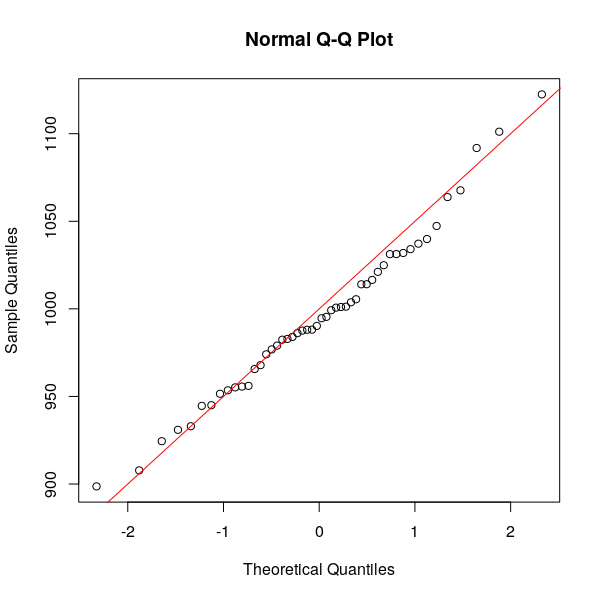
\includegraphics[width=.45\textwidth]{sampling-qqplot-good}
    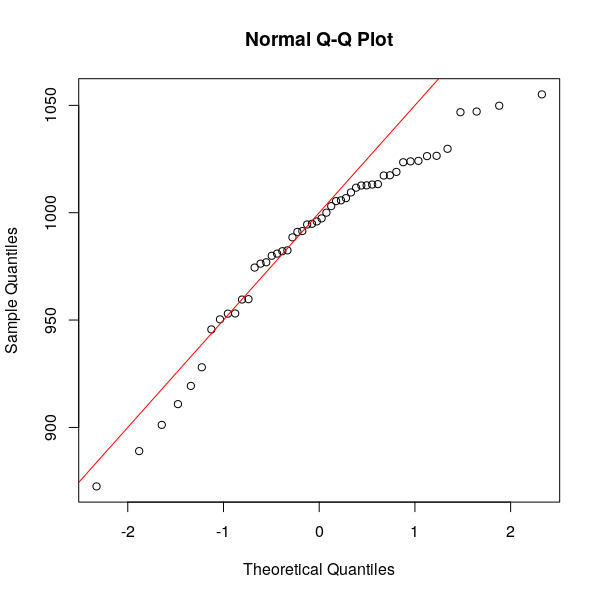
\includegraphics[width=.45\textwidth]{sampling-qqplot-bad}
  \end{center}
  \caption{De QQ-plot links is gebaseerd op een steekproef van 50 observaties uit een normale distributie met gemiddelde 1000 en standaardafwijking 50. De rechterplot is gebaseerd op een Student-$t$ distributie met 15 vrijheidsgraden. Het aantal observaties, gemiddelde en standaardafwijking zijn hetzelfde als links.
    De lijnen in het rood duiden aan waar zich in theorie de observaties zouden moeten bevinden. Links is dat min of meer zo, maar rechts wijken de observaties af, vooral in de extremen.}
  \label{fig:qqplot}
\end{figure}

\lstinputlisting{data/qqplot.R}

\section{Centrale limietstelling}
\label{sec:centrale-limietstelling}

\begin{definition}[Lineaire combinatie van onafhankelijke, gelijk verdeelde stochasten]
Formeel: Een lineaire combinatie van onafhankelijke, gelijk verdeelde stochasten is steeds normaal verdeeld.

\[X_{i} \sim Nor(\mu_{i}, \sigma_{i}) \Rightarrow Y = \sum_{i} \alpha_{i} X_{i} \textnormal{ ook normaal verdeeld} \]

Bijgevolg zal ook het steekproefgemiddelde van een steekproef uit een populatie met een willekeurige verdeling, nagenoeg normaal verdeeld zijn voor een voldoende grote $n$.
\end{definition}

Wanneer men dus een aselecte steekproef neemt van onafhankelijke variabelen met een normale verdeling, dan zegt de centrale limietstelling dat het gemiddelde van deze steekproef bij benadering normaal verdeeld zal zijn. Dus als men steeds opnieuw een steekproef neemt met dezelfde grootte, en telkens het gemiddelde optekent, bekomt men bij benadering de grafiek van een normale verdeling. Hoe groter de steekproef, hoe beter de benadering. Het steekproefgemiddelde is dus normaal verdeeld, onafhankelijk van de onderliggende verdeling van de grootheid waarvan men een steekproef neemt. Algemeen kunnen we volgende stelling poneren:

\begin{definition}[Centrale limietstelling]
Beschouw een aselecte steekproef van $n$ waarnemingen die uit een populatie met verwachtingswaarde $\mu$ en standaardafwijking $\sigma$ wordt genomen. Als $n$ groot genoeg is zal de kansverdeling van het steekproefgemiddelde $\overline{x}$ een normale verdeling benaderen met verwachting $\mu_{\overline{x}} = \mu$ en standaardafwijking $\sigma_{\overline{x}} = \frac{\sigma}{\sqrt{n}}$. Hoe groter de steekproef is, des te beter zal de kansverdeling van $\overline{x}$ de verwachtingswaarde van de populatie benaderen.

\end{definition}

Bij het afnemen van een steekproef is zelden de onderliggende verdeling gekend, en toch kan men uitspraken doen over de gemiddelde waarde. Dit is volledig te danken aan de centrale limietstelling, die dit gemiddelde een regel oplegt los van de onderliggende kansverdeling. De centrale limietstelling houdt het steekproefgemiddelde in bedwang, sluit het op in de Gaussische kooi waaruit het nooit kan ontsnappen. Dit, en alleen dit, laat wetenschappers toe het nauwkeurig te bestuderen, te observeren en stelt hen in staat te concluderen.

Want, mocht de verdeling van het steekproefgemiddelde afhankelijk zijn van de onderliggende verdeling, een resultaat dat men tot op zekere hoogte zelfs zou verwachten, zou het onmogelijk zijn om concrete uitspraken te doen over vele wetenschappelijke resultaten. In de theoretische statistiek duiken vrijwel constant limieten van steekproefgemiddeldes op, en deze kunnen dankzij de centrale limietstelling zonder verpinken vervangen worden door een normale verdeling. Zou dit niet mogelijk zijn, dan zou de ganse theorie rond het schatten van parameters in elkaar storten wat dan weer rampzalig zou zijn voor de praktijk. Onderzoeken vergelijken zou herleid worden tot een quasi onmogelijke opgave, en de statistiek in het algemeen zou veel lastiger en ingewikkelder worden.

\subsection{Toepassing van de centrale limietstelling}
Bij het trekken van een aselecte steekproef van omvang $n$ uit een populatie met (onbekend) gemiddelde $\mu$ en standaarddeviatie $\sigma$ is de kansverdeling van het steekproefgemiddelde een kansvariabele $M \sim N (\overline{x}, \frac{\sigma}{\sqrt{n}})$, op voorwaarde dat de steekproefomvang voldoende groot is.

\begin{example}
  We bekijken nu de reactiesnelheid van al onze superhelden en uit onze steekproef met $n = 100$ en $\overline{x} = 90, \sigma = 60$ (miliseconden). Dan kunnen we ons de vraag stellen: wat is de kans dat de gemiddelde reactiesnelheid van een superheld minder is dan $104 ms$?


  \begin{enumerate}
    \item De kansvariabele hier is de gemiddelde reactiesnelheid $\overline{x}$ in een steekproef van $n=100$ superhelden. Daarom geldt wegens de centrale limietstelling:
    \[ \overline{x} \sim Nor(\mu = 90, \sigma_{\overline{x}} = \frac{60}{\sqrt{100}} = 6) \]
    \item We kunnen hierbij de passende $z$-score bepalen:
    \[ z = \frac{104-90}{\frac{60}{\sqrt{100}}} = \frac{104-90}{6} = 2,33 \]
    Dus geldt : $P(\overline{x} < 104) = P(Z < 2,33) = 1 - 0,0099 \approx 0,99$
  \end{enumerate}
\end{example}

\subsection{Schatten van een parameter}

Indien we nu een steekproef onderzoeken, willen we uit de berekening op de steekproef een aantal conclusies kunnen trekken met betrekking tot de populatie. We willen bijvoorbeeld de gemiddelde kracht kennen van een superheld of de fractie superhelden die rijk zijn. Als we een schatting geven voor dergelijke onbekende parameter, noemen we dat ook een puntschatter. We gebruiken bijvoorbeeld $\overline{x}$ als schatter om $\mu$ te schatten.

\begin{definition}[puntschatter]
  Een puntschatter voor een populatieparameter is een regel of een formule die ons zegt hoe we uit de steekproef een getal moeten berekenen om de populatieparameter te schatten.
\end{definition}

\subsection{Betrouwbaarheidsinterval populatiegemiddelde bij grote steekproef}
\label{ssec:betrouwbaarheidsinterval-grote-steekproef}

In het geval het schatten van een gemiddelde van een populatie uit een steekproef hebben we totaal geen idee over hoe correct onze schatting is. Daarvoor gaan we op zoek naar een interval waarvan we met een bepaalde zekerheid, bv. 95\%, kunnen zeggen dat het de te schatten karakteristiek bevat.

\begin{definition}[Betrouwbaarheidsinterval]
Een betrouwbaarheidsinterval is een regel of een formule die ons zegt hoe we uit de steekproef een interval moeten berekenen dat de waarde van de parameter met een bepaalde hoge waarschijnlijkheid bevat.
\end{definition}

Een eerste goede schatting voor populatiegemiddelde zou het steekproefgemiddelde zijn:

\[ \overline{x} = \frac{1}{n} \sum_{i} x_{i} \]

Natuurlijk is deze schatting niet de werkelijke waarde van de populatie. Daarom wordt vaak rondom $\overline{x}$ een interval geconstrueerd dat de waarden bevat die aannemelijk zijn voor $\mu$. Hiervoor kunnen we gebruik maken van de centrale limietstelling: het gemiddelde in een te trekken steekproef van omvang $n$ is normaal verdeeld met karakteristieken $\mu$ en $\frac{\sigma}{\sqrt{n}}$.  Als we nu het gemiddelde standaardiseren krijgen we:

\[ Z = \frac{\overline{x} - \mu}{\frac{\sigma}{\sqrt{n}}} \]

Deze uitdrukking hangt van $\mu$ af maar we weten wel dat deze standaardnormaal verdeeld is. We kunnen daarom getallen $-z$ en $z$ vinden, onafhankelijk van $\mu$, waartussen $Z$ met een gekozen kans $1 - \alpha$ ligt. Deze kans $1 - \alpha$ wordt het \emph{betrouwbaarheidsniveau}\index{betrouwbaarheidsniveau}\index{niveau!betrouwbaarheids-} genoemd. We nemen hier $1 - \alpha= 0,95$.

\[P(-z < Z < z) = 1 - \alpha = 0,95 \]

Hieruit halen we dat $\alpha = 0,05$. Door het toepassen van de symmetrieregel weten we dus dat we volgende term moeten berekenen:

\[ P( Z < z) = 1 - 0,025 \]

Kijken we in de Z-tabel dan vinden we voor de rechterstaartkans $0,025$ de z-score van $1,96$.

Dus vinden we :

\[ P( -1,96 < \frac{\overline{x} - \mu}{\frac{\sigma}{\sqrt{n}}} < 1,96 ) \]
en dus
\[ P ( \overline{x} -1,96 \frac{\sigma}{\sqrt{n}} <\mu < \overline{x} + 1,96 \frac{\sigma}{\sqrt{n}}) \]

Op die manier kunnen we dus grenzen bepalen die een interval aanduidt waar 95\% kans is dat $\mu$ gevonden wordt. Formeel: als je herhaalde steekproeven zou nemen en telkens op basis van het gerealiseerde steekproefgemiddelde $\overline{x}$ een betrouwbaarheidsinterval zou maken, dan zal bij 95\% van de intervallen $\mu$ binnen de intervalgrenzen liggen.

Opgelet, we gaan er hier van uit dat we de standaarddeviatie van de populatie kennen, wat meestal niet zo is. Indien de steekproef groot genoeg is, kunnen we de steekproefstandaarddeviatie nemen als schatter voor de standaarddeviatie voor de populatie.

\[ P ( \overline{x} -1,96 \frac{\sigma_{\overline{x}}}{\sqrt{n}} < \mu < \overline{x} + 1,96 \frac{\sigma_{\overline{x}}}{\sqrt{n}}) \]


\begin{figure}[t]
\centering
\begin{tikzpicture}
\begin{axis}[
  domain=-3:3, samples=100,
  axis lines*=left, xlabel=$z$,
  every axis y label/.style={at=(current axis.above origin),anchor=south},
  every axis x label/.style={at=(current axis.right of origin),anchor=west},
  height=5cm, width=12cm,
  xtick={-1.96,0,1.96}, ytick=\empty,
  enlargelimits=false, clip=false, axis on top,
  grid = major
  ]
  \addplot [fill=cyan!20, draw=none, domain=-3:3] {gauss(0,1)} \closedcycle;
  \draw [yshift=-0.6cm, latex-latex](axis cs:-1.96,0) -- node [fill=white] {$\sigma$} (axis cs:1.96,0);
\end{axis}
\end{tikzpicture}
\caption{Standaardnormale verdeling die 95\% betrouwbaarheidsinterval aanduidt.}
\label{fig:verdelingStandaardnormaal}
\end{figure}

\subsection{Betrouwbaarheidsinterval populatiegemiddelde bij een kleine steekproef}
\label{ssec:betrouwbaarheidsinterval-kleine-steekproef}

Bij kleine steekproeven kunnen we niet langer veronderstellen dat de kansverdeling van $\overline{x}$ bij benadering
normaal verdeel is, omdat de centrale limietstelling alleen normaliteit garandeert voor grote steekproeven ($n >30$). De vorm
van de kansverdeling van het steekproefgemiddelde $\overline{x}$ hangt nu af van de vorm van de verdeling van de populatie waaruit de
steekproef genomen wordt. Alhoewel nog steeds geldt dat $\sigma_{\overline{x}} = \frac{\sigma}{\sqrt{n}}$ kan
de standaardafwijking $s$ een slechte benadering zijn voor $\sigma$ als de steekproef klein is.

Als oplossing kunnen we een nieuwe grootheid bepalen. In plaats van

\[ z = \frac{\overline{x} - \mu}{\frac{\sigma}{\sqrt{n}}} \]

construeren we

\[ t = \frac{\overline{x} - \mu}{\frac{s}{\sqrt{n}}} \]

Deze heeft een kansverdeling die beschreven wordt door een Student-t verdeling. Deze lijkt zeer goed op de normale verdeling: klokvormig, symmetrisch en met verwachtingswaarde 0.

De precieze vorm van de kansverdeling $t$ hang af van de steekproefomvang $n$. We zeggen dat de t-verdeling $(n-1)$ vrijheidsgraden heeft (afgekort $df$).
Merk op dat:
\begin{itemize}
  \item $(n-1)$ ook gebruikt werd om $s^{2}$ te berekenen
  \item als $n \rightarrow \infty$ we de standaardnormale verdeling verkrijgen.
\end{itemize}

Indien we nu een betrouwbaarheidsinterval willen bepalen voor een steekproef met een klein aantal waarden moeten we het volgende doen:

\begin{definition}[Betrouwbaarheidsinterval kleine steekproef]
  Om een betrouwbaarheidsinterval voor het gemiddelde te bepalen op basis van een klein steekproef bepalen we:
  \[ \overline{x} \pm t_{\frac{\alpha}{2}}(\frac{s}{\sqrt{n}}) \]
  waarbij $t_{\frac{\alpha}{2}}$ gebaseerd is op $(n-1)$ vrijheidsgraden. We veronderstellen wel dat we een aselecte steekproef genomen hebben uit
  een populatie die bij benadering normaal verdeeld is.
\end{definition}

\begin{table}
  \centering
  \begin{tabular}{ll}
  	\textbf{Functie} & \textbf{Betekenis}                                             \\ \midrule
  	\verb|pt(x, df)| & Linkerstaartkans, $P(X<\mathtt{x})$                            \\
  	\verb|dt(x, df)| & Hoogte van de curve op punt \texttt{x}                         \\
  	\verb|qt(p, df)| & Onder welke grens zal \texttt{p}\% van de waarnemingen liggen? \\
  	\verb|rt(n, df)| & Genereer \texttt{n} random getallen volgens deze verdeling
  \end{tabular}

  \caption{Kansberekeningsfuncties in R voor de Student-$t$ verdeling met \texttt{df} vrijheidsgraden, verwachte waarde 0 en standaardafwijking 1.}
  \label{tab:t-prob-r}
\end{table}

\subsection{Betrouwbaarheidsinterval voor populatiefractie bij een grote steekproef}
\label{ssec:betrouwbaarheidsinterval-populatiefractie}

Indien je een variabele wil meten als een fractie, bijvoorbeeld \% mensen die ja geantwoord heeft op een bepaalde vraag, dan willen we in feite de kans $p$ op succes in een bernouilli experiment schatten, waarbij $p$ de kans is dat een willekeurig geselecteerde respondent (of element van de populatie) een succes is (succes in termen van binomiaal experiment). We kunnen $p$ dan schatten door bijvoorbeeld:

\[ \overline{p} = \frac{\textnormal{aantal successen}}{n} \]

Om nu de betrouwbaarheid van de schatter $\overline{p}$ te bepalen moeten we de kansverdeling kennen van $\overline{p}$. Dit kunnen we beredeneren door toepassing van de centrale limietstelling op het gemiddelde aantal successen in de steekproef van omvang $n$. Indien succes = 1 en faling = 0, dan hebben we een steekproef van $n$ elementen, ieder met dezelfde verdeling (kans op 1 is $p$ en kans op 0 is $q=1-p$).  Het gemiddelde $\overline{p}$ heeft dan bij benadering een normale verdeling. Of dus:

\begin{itemize}
  \item Verwachting van kansverdeling van $\overline{p}$ is $p$.
  \item De standaardafwijking van kansverdeling $\overline{p} = \sqrt{\frac{pq}{n}}$
  \item Voor grote steekproeven is $\overline{p}$ bij benadering normaal verdeeld.
\end{itemize}

Aangezien $\overline{p}$ een steekproefgemiddelde is van het aantal successen, stelt dit ons in staat een betrouwbaarheidsinterval te berekenen analoog als die voor de intervalschatting van $\mu$ voor grote steekproeven.

\begin{definition}[Betrouwbaarheidsinterval voor $p$ gebaseerd op grote steekproef]
  \[ \overline{p} \pm z_{\frac{\alpha}{2}} \sqrt{\frac{\overline{p}\overline{q}}{n}} \]
  met $\overline{p} = \frac{x}{n}$ en $\overline{q} = 1- \overline{p}$
\end{definition}


\section{R}
We kijken naar enkele basisoperaties die verband houden met enkele distributies. Er zijn een groot aantal verdelingen beschikbaar, maar we kijken maar naar een paar. Als u wilt weten welke distributies beschikbaar zijn, kunt u een zoekopdracht uitvoeren met behulp van de opdracht

\begin{lstlisting}
> help.search ("distribution").
\end{lstlisting}


Hier geven we details over de commando's die verband houden met de normale distributie en vermelden kort de commando's voor andere distributies. De functies voor verschillende verdelingen zijn zeer vergelijkbaar.

De prefixen zijn als volgt:
\begin{description}
	\item[d] geeft de hoogte van de respectievelijke kansdichtheidsfunctie
	\item[p] geeft de cumulatieve kansdichtheidsfunctie
	\item[q] geeft de omgekeerde cumulatieve dichtheidsfunctie
	\item[r] geeft een willekeurige waarde
\end{description}

\subsection{De normale verdeling}
Er zijn vier functies die kunnen worden gebruikt om de waarden geassocieerd met de normale distributie te genereren.
\subsubsection{dnorm}

De eerste functie waarnaar we kijken, is \texttt{dnorm}. Gegeven een waarde geeft het de hoogte van de kansverdeling op elk punt terug. Als u alleen de punten zonder gemiddelde en standaardafwijking ingeeft wordt een gemiddelde van nul en standaardafwijking van 1 beschouwd. Er zijn opties om verschillende waarden voor de gemiddelde en standaardafwijking te gebruiken.

\lstinputlisting{data/norm.R}

\subsubsection{pnorm}

Dit is de cumulatieve kansdichtheidsfunctie, of anders gezegd de linkerstaartkans: \texttt{pnorm(x)} is $P(Z < x)$.

\subsubsection{qnorm}
De volgende functie die we bekijken is \texttt{qnorm}, die de inverse van \texttt{pnorm} is. Het idee achter \texttt{qnorm} is dat je het een kans $\alpha$ geeft, en het geeft het getal weer waarvan de cumulatieve distributie overeenkomt met de waarschijnlijkheid $\alpha$.

\subsubsection{rnorm}

\lstinputlisting{data/qnorm.R}
De laatste functie die we onderzoeken is de \texttt{rnorm} functie die willekeurige getallen kan genereren waarvan de distributie normaal is. Het argument dat je ingeeft is het aantal willekeurige getallen dat u wilt, met optionele argumenten om de gemiddelde en standaardafwijking op te geven:

\lstinputlisting{data/rnorm.R}

\section{Oefeningen}
\label{sec:steekproefonderzoek-oefeningen}

\begin{exercise}
  \label{ex:prob-norm-dist}
  Bereken ook elke keer het gevraagde gebied.
  \begin{enumerate}[label=\alph*.]
    \item $P(Z < 1.33)$
    \item $P(Z > 1.33)$
    \item $P(Z < -1.33)$
    \item $P(Z > -1.33)$
    \item $P(Z < 0.45)$
    \item $P(Z > -1.05)$
    \item $P(Z < 0.65)$
    \item $P(-0.45 < Z < 1.20)$
    \item $P(-1.35 < Z < -0.10)$
    \item $P(-2.10 < Z < -0.90)$
  \end{enumerate}
\end{exercise}

\begin{exercise}
	Bepaal de dichtheid en de cumulatieve waarschijnlijkheidscurve voor een normale verdeling met een gemiddelde $\mu$
	van 2,5 en $\sigma = 1,5$. Bepaal de oppervlakte voor het gebied onder de dichtheidscurve tussen
	$x = 0.5$ en $x = 4$. Controleer uw antwoord door de berekening te doen.
\end{exercise}

\begin{exercise}
	Bepaal de dichtheid en de cumulatieve waarschijnlijkheidscurve voor een t-verdeling met $df = 3$. Teken ook een normale verdeling met een $\mu = 0$  en $\sigma = 1$.
\end{exercise}

\begin{exercise}
Gebruik de functie \verb|rnorm()| een willekeurige steekproef van 25 waarden uit een normale verdeling te tekenen met een gemiddelde van 0 en een standaardafwijking gelijk aan 1,0. Gebruik een histogram, met \verb|probability = TRUE|.

Maak een overlay over het histogram met: (a) de theoretische dichtheidscurve voor een normale verdeling met gemiddelde 0 en standaardafwijking gelijk aan 1,0; (b) een ``geschatte'' dichtheidscurve op basis van het gemeten steekproefgemiddelde en -standaardafwijking.

Herhaal dit voor een steekproef van 100 en 500 waarden.
\end{exercise}

\begin{exercise}
  In de  Hogeschool zijn er twee klassen voor het vak onderzoekstechnieken. De studenten werden willekeurig over de klassen verdeeld, zodat we mogen veronderstellen dat de ene klas niet slimmer is dan de andere. In de A-klas geeft mevr. X les, in de B-klas geeft mr. Y les. X is nogal streng en op het einde van het schooljaar behaalt haar klas een gemiddelde van 54 op 100 met een standaardafwijking van 11.

  Y is iets losser en stimuleert de leerlingen al gauw met een puntje meer. Op het einde van het schooljaar behaalt zijn klas een gemiddelde van 62 op 100 en een standaardafwijking van 7.

  Wouter zit in de A-klas en heeft $\frac{63}{100}$ voor wiskunde. Stijn zit in de B-klas en behaalt $\frac{67}{100}$. Wie heeft volgens jou het beste gescoord binnen de eigen klas?
\end{exercise}

\begin{exercise}
  Een gezondheidsonderzoek tussen 1988 en 1994 gaf aan dat de gemiddelde cholesterolwaarde bij vrouwen tussen 20 en 29 jaar 183 mg/dl bedroeg, met een standaardafwijking gelijk aan 36. We nemen nu een aselecte steekproef van 81 vrouwen. Los volgende vragen op:

  \begin{enumerate}[label=\alph*.]
    \item Schets de kansdichtheidsfunctie voor de populatie en de kansverdeling van het steekproefgemiddelde $\overline{x}$.
    \item Bepaald de kans dat $\overline{x}$ kleiner is dan 185.
    \item Bepaal de kans dat $\overline{x}$ tussen 175 en 185 ligt.
    \item Bepaal de kans dat $\overline{x}$ groter is dan 190.
  \end{enumerate}
\end{exercise}

\begin{exercise}
  Een aselecte steekproef van 64 stuks wordt getrokken uit een populatie met onbekende verdeling. De verwachting en de standaardafwijking van de populatie
  zijn wel gekend: $\mu = 20$ en $\sigma=16$. Los volgende vragen op:

  \begin{enumerate}[label=\alph*.]
    \item Bepaal de verwachting en standaardafwijking van het steekproefgemiddelde.
    \item Beschrijf de vorm van de verdeling van het steekproefgemiddelde. In hoeverre hangt je antwoord af van de grootte van de steekproef?
    \item Bereken de $z$ score bij $\overline{x_{1}} = 15.5$ en $\overline{x_{2}} = 23$.
    \item Bepaal kans dat $\overline{x} <16$.
    \item Bepaal kans dat $\overline{x} > 23$.
    \item Bepaal kans dat $16< \overline{x}< 22$.
  \end{enumerate}
\end{exercise}

\begin{exercise}
  Verkeersdrempels zijn bedoeld om de snelheid van automobilisten te be\"invloeden. Afhankelijk van de gewenste snelheid in een straat worden de drempels steiler of minder steil gemaakt. Drempel A is zo ontworpen dat 85 \% van de automobilisten de drempel passeert met een snelheid van minder dan 50 km per uur. In de praktijk blijkt dat de passeersnelheid bij een drempel normaal verdeeld is. Bij drempel A werd een gemiddelde passeersnelheid van 43,1 km/h gevonden met standaardafwijking 6,6 km/h.

  \begin{enumerate}[label=\alph*.]
    \item Toon aan dat 85\% van de automobilisten niet harder dan 50 km/h rijdt.
    \item Bij hoeveel van de 1200 metingen kan, op grond van eerdere ervaringen, een snelheid van meer dan 55 km/h worden verwacht?
  \end{enumerate}
\end{exercise}

\begin{exercise}
  Een conservenfabrikant krijgt de laatste tijd klachten over de netto inhoud van zijn conserven met wortelen en erwtjes, die volgens de verpakking netto 1 liter zouden moeten bevatten. Daarom laat hij een steekproef nemen waarin de netto inhoud van 40 willekeurig gekozen blikjes wordt gecontroleerd. De resultaten worden samengevat in Tabel~\ref{tab:Steekproefwaarden}.

Vraag A:
\begin{itemize}
  \item Vul de tabel aan met de cumulatieve absolute frequentie
  \item Vul de tabel aan met de relatieve frequentie
  \item Vul de tabel aan met de cumulatieve relatieve frequentie.
\end{itemize}
Vraag B:

\begin{itemize}
  \item Bereken het gemiddelde
  \item Bereken de standaardafwijking
  \item Hoeveel procent van de blikken bevatten te weinig wortelen en erwtjes.
  \item Teken een histogram van de absolute frequentie.
  \item Zijn de gegevens normaal verdeeld?  Hoe zie je dat?
\end{itemize}

\end{exercise}

  \begin{table}
  \centering
  \begin{tabular}{lr}
    \toprule
    Inhoud & $n_{i}$ \\
    \midrule
    $[970,980[$ & 3 \\
    $[980,990[$ & 5 \\
    $[990,1000[$ & 13 \\
    $[1000,1010[$ & 11 \\
    $[1010,1020[$ & 5 \\
    $[1020,1030[$ & 3 \\
    \bottomrule
  \end{tabular}
  \caption{Steekproefwaarden}
  \label{tab:Steekproefwaarden}
\end{table}

\begin{exercise}
  Een webhostingfirma heeft een Service Level Agreement met een klant voor een gegarandeerde uptime van ``five nines'' (99,999\%).  Die wordt aan het einde van elk jaar gecontroleerd en als de minimale uptime niet gehaald wordt, moet de hostingfirma een boete betalen.

  Om de uptime te meten, voert een monitoringsysteem elke minuut een \texttt{HTTP GET /} uit en controleert het resultaat a.h.v.
  de HTTP return code. In de maand januari is er één enkele HTTP request onsuccesvol geweest.

  \begin{itemize}
    \item Als deze trend zich voortzet, wat is de kans dat de SLA niet gehaald wordt aan het einde van het jaar? Gebruik de formule voor de kansverdeling van een fractie.
    \item De gebruikte formule is eigenlijk niet geschikt in dit specifieke geval en geeft een vertekend beeld. Wat zou de reden kunnen zijn?
  \end{itemize}
\end{exercise}

\section{Antwoorden op geselecteerde oefeningen}
\label{sec:oplossingen-steekproefonderzoek}

\paragraph{Oefening \ref{ex:prob-norm-dist}}

\begin{enumerate}[label=\alph*.]
  \item $0,908$
  \item $0,092$
  \item $0,092$
  \item $0,908$
  \item $0,674$
  \item $0,853$
  \item $0,742$
  \item $0,559$
  \item $0,372$
  \item $0,166$
\end{enumerate}

\chapter{Toetsingsprocedures}
\label{ch:toetsingsprocedures}

In de voorbije hoofdstukken hebben we gezien hoe we aan de hand van steekproefonderzoek bepaalde kerngetallen over een populatie kunnen berekenen, bijvoorbeeld aan de hand van puntschatters of betrouwbaarheidsintervallen. We kunnen deze informatie ook gebruiken om bepaalde hypothesen over een populatie te toetsen. Een hypothese is een veronderstelling waarvan nog bewezen moet worden dat ze correct is. Het doel van een toetsingsprocedure is het testen van een hypothese omtrent de waarden van 1 of meerdere populatieparameters.

\begin{definition}[Statistische hypothese.]
  Een statistische hypothese\index{hypothese!statistische} is een uitspraak over de numerieke waarde van een populatieparameter.
\end{definition}

Voorbeelden van hypothesen:

\begin{itemize}
  \item Gemiddeld redt een superheld minstens 3,3 mensen per dag.
  \item De gemiddelde lengte van een superheld is minstens 120 cm.
  \item \dots
\end{itemize}

In dit hoofdstuk gaan we de algemene theorie over toetsen formuleren aan de hand van het testen van hypothesen over het populatiegemiddelde $\mu$, de $z$-toets. Naast de $z$-toets bestaan er echter nog vele andere statistische hypothesetoetsen die in specifieke situaties gebruikt kunnen worden. De meest geschikte statistische toets hang o.a.~af van de populatiegrootheid in kwestie (gemiddelde, standaardafwijking, enz.), en veronderstellingen over de onderliggende stochastische verdeling van de populatie (normaal verdeeld of niet, enz,).

\section{Leerdoelen}
\label{sec:toetsingsprocedures-leerdoelen}

Na dit hoofdstuk moet je in staat zijn om:

\begin{itemize}
  \item De volgende begrippen uit dit hoofstuk uit te leggen:
  \begin{itemize}
    \item hypothesetoets, statistische hypothese, nulhypothese, alternatieve hypothese;
    \item teststatistiek, aanvaardings- en verwerpingsgebied, overschrijdingskans;
    \item $z$-toets, $t$-toets, linkszijdig, rechtszijdig, tweezijdige;
    \item Type I en Type II-fouten;
  \end{itemize}
  \item De algemene procedure voor een statistische toets te beschrijven;
  \item Uit de beschrijving van een situatie waarbij gevraagd wordt om een uitspraak over een populatiegemiddelde te verifiëren:
  \begin{itemize}
    \item te bepalen of er een $z$- of $t$-toets mag toegepast worden;
    \item uit de onderzoeksvraag af te leiden of de links-, rechts- of tweezijdige variant moet gebruikt worden;
  \end{itemize}
  \item Op een gegeven situatie correct de $z$- of $t$-toets toe te passen, d.w.z.:
  \begin{itemize}
    \item De nul- en alternatieve hypothese te formuleren (wiskundige notatie);
    \item De teststatistiek te berekenen;
    \item De kritieke grenswaarde(n) te berekenen en te bepalen of de teststatistiek in het aanvaardings- of verwerpingsgebied ligt;
    \item De overschrijdingskans te berekenen;
    \item Een correct besluit te kunnen trekken (nulhypothese verwerpen of niet);
    \item Een antwoord te formuleren op de onderzoeksvraag.
  \end{itemize}
\end{itemize}

\section{Elementen van een hypothesetoets}
\label{sec:elementen-hypothesetoets}

Algemeen gezien bestaat een toetsingsprocedure uit 4 elementen:
\begin{enumerate}
  \item \textbf{Nulhypothese}\index{nulhypothese}\index{hypothese!nul-} $H_{0}$: Deze hypothese proberen we te ontkrachten door een redenering in het ongerijmde. We gaan deze hypothese accepteren, tenzij de observaties uit de steekproef overtuigend wijzen op het tegendeel.
  \item \textbf{Alternatieve hypothese}\index{hypothese!alternatieve} $H_{1}$: Dit is meestal de hypothese die de onderzoeker wil bewijzen. Deze hypothese zal echter alleen worden geaccepteerd als de observaties uit de steekproef overtuigend wijzen op de juistheid ervan.
  \item \textbf{Teststatistiek}: De veranderlijke die berekend wordt uit de steekproef
  \item Aanvaardings- en kritiek gebied:
  \begin{itemize}
    \item  \textbf{Aanvaardingsgebied\index{aanvaardingsgebied}\index{gebied!aanvaardings-}}: Het gebied van waarden die de nulhypothese $H_{0}$ ondersteunt
    \item \textbf{Verwerpingsgbied\index{verwerpingsgebied}\index{gebied!verwerpings-}}: gebied dat waarden bevat die de nulhypothese verwerpen. Ook kritiek gebied\index{gebied!kritiek} genoemd.
  \end{itemize}
\end{enumerate}

Een alternatief voor de laatste stap is het berekenen van de \emph{overschrijdingskans} (zie verder).

De beslissing om de nulhypothese $H_{0}$ te verwerpen of te aanvaarden is gebaseerd op informatie uit een steekproef, getrokken uit de populatie waarover de hypothese is geformuleerd. De steekproefwaarden worden gebruikt om 1 enkele waarde van een teststatistiek te berekenen die de beslissing zal bepalen. Daartoe worden alle waarden die de teststatistiek kan aannemen, verdeeld in twee gebieden, enerzijds het aanvaardingsgebied en anderzijds het verwerpingsgebied. Indien de waarde van de teststatistiek ligt in het verwerpingsgebied, dan wordt de nulhypothese verworpen en de alternatieve hypothese aanvaard. Indien de waarde van de teststatistiek in het aanvaardingsgebied valt dan wordt de nulhypothese aanvaard.

\section{Toetsingsprocedure voor de \texorpdfstring{$z$}{z}-toets}
\label{sec:toetsingsprocedure-z-toets}

In de eerste toetsingsprocedure die we in deze cursus uitwerken, gaan we een uitspraak over het populatiegemiddelde $\mu$ verifiëren. Deze is algemeen bekend als de $z$-toets\index{$z$-toets}\index{toets!$z$-}.

\begin{enumerate}
  \item De vermoedens over de populatie worden vastgelegd in twee hypothesen $H_{0}$ en $H_{1}$. Voor de (rechtszijdige) $z$-toets is de nulhypothese dat het populatiegemiddelde $\mu$ een bepaalde waarde heeft, en de alternatieve hypotehese dat $\mu$ \emph{groter} is.
  \item Het significantieniveau\index{significantieniveau}\index{niveau!significantie-} $\alpha$ en steekproefomvang $n$ worden vastelegd. Je kan $\alpha$ in principe zelf kiezen (bv. 0,05)\footnote{Merk op dat het significantieniveau gerelateerd is aan het betrouwbaarheidsniveau $1-\alpha$. Zie Sectie~\ref{ssec:betrouwbaarheidsinterval-grote-steekproef}}. Hoe dichter het significantieniveau bij 0 ligt, hoe minder twijfel er is over het resultaat van de toets. Maar langs de andere kant wordt het ook moeilijker om de nulhypothese te verwerpen.
  \item De waarde van de toetsingsgrootheid in de steekproef wordt berekend. De uitkomst is bepalend voor de beslissing of we de nulhypothese $H_{0}$ kunnen verwerpen of niet. We weten dankzij de centrale limietstelling dat de kansverdeling van het steekproefgemiddelde $M \sim Nor( \mu, \frac{\sigma}{\sqrt{n}})$.
  \item Het kritieke gebied bepalen, of meer bepaald de grens tussen het aanvaardings- en het verwerpingsgebied. We zoeken een grenswaarde\index{kritieke grenswaarde} $g$ zodat:
  
  \begin{align}
  P(M > g) = \alpha & \Leftrightarrow P\left(Z> z=\frac{g-\mu}{\sigma/\sqrt{n}}\right) = \alpha & \mathrm{(normalisatie)}\\
  & \Leftrightarrow P\left(Z < z = \frac{g-\mu}{\sigma/\sqrt{n}}\right) = 1-\alpha & \mathrm{(100\%-regel)}
  \end{align}
  
  De $z$-waarde hangt af van het gekozen significantieniveau en kan worden opgezocht in een $z$-tabel of berekend worden met de R-functie \texttt{qnorm(1-alpha)}. Daaruit kunnen we dan $g$ afleiden:
  
  \begin{equation}
  z = \frac{g-\mu}{\sigma/\sqrt{n}} \Leftrightarrow g = \mu + z \frac{\sigma}{\sqrt{n}}
  \label{eq:kritieke-grenswaarde-z-toets}
  \end{equation}

  Alle waarden \emph{links} van $g$ vormen het aanvaardingsgebied. Waarden rechts, die dus ver van het $H_0$ veronderstelde populatiegemiddelde liggen, zijn het verwerpingsgebied. Zie ook Sectie~\ref{sec:kritieke-gebied}.
\end{enumerate}

\begin{example}
  \label{ex:hypothesetoets-dagelijkse-reddingen}
  Algemeen wordt aangenomen dat superhelden gemiddeld 3,3 mensen per dag redden. De onderzoekers krijgen echter gevoel dat dat niet zo is: ze hebben de indruk dat een superheld \emph{meer} dan $3,3$ mensen per dag redt.
  
  Ze gaan dit onderzoeken en voeren een steekproef uit bij $n = 30$ superhelden. In deze steekproef is het gemiddelde $\overline{x} = 3,483$ is. De standaardafwijking in de populatie is verondersteld gekend en is $\sigma = 0,55$.
  
  Kan hieruit besloten worden dat superhelden gemiddeld meer dan 3,3 mensen per dag redt?

  \begin{enumerate}
    \item We veronderstellen dat het aantal mensen dat een superheld redt normaal verdeeld  is en formuleren twee hypothesen omtrent de parameter $\mu$.
    \begin{itemize}
      \item $H_{0}$ = de nulhypothese (hetgeen we willen weerleggen). In dit geval \[ H_{0} : \mu = 3,3 \]
      \item $H_{1}$ = alternatieve hypothese (vermoeden dat we willen aantonen). In dit geval \[H_{1}= \mu > 3,3 \]
    \end{itemize}
  
    We veronderstellen in de redenering initieel dat de nulhypothese $H_{0}$ waar is. Indien het gemiddelde aantal mensen gered per dag $\overline{x}$ van de steekproef sterk afwijkt van de veronderstelde waarde, verwerpen we de nulhypothese $H_{0}$ en aanvaarden we de alternatieve hypothese $H_{1}$.
    
    Wat betekent nu ``sterk afwijken''? Zou je uit een populatie met gemiddelde van $3,3$ gemakkelijk een steekproef kunnen trekken met gemiddelde $3,483$? De centrale limietstelling (zie Sectie~\ref{sec:centrale-limietstelling}) laat ons toe de kans hiertoe te berekenen.
    
    \item Vastleggen significantieniveau $\alpha$ en steekproefomvang $n$. We willen een significantieniveau van 5\% kiezen, dus $\alpha = 0,05$. De steekproefomgang is gegeven en is hier $n = 30$.
    
    \item De waarde van de toetsingsgrootheid in de steekproef bepalen. We nemen hier het steekproefgemiddelde: $\overline{x} = 3,483$
    
    We veronderstellen in de redenering dat de nulhypothese $H_{0}$ waar is en dat we $\sigma$ goed kunnen schatten hebben ($\sigma = 0,55$). Dan geldt voor het steekproefgemiddelde $M$ volgens de centrale limietstelling dat:
    
    \[M \sim  Nor(\mu = 3,3; \sigma = \frac{0,55}{\sqrt{30}})\]
    
    De waarde $\overline{x} = 3,483$ bevindt zich erg rechts (zie Figuur~\ref{fig:hypothesetoets-reddingen-per-dag}). $\overline{x}$ ligt zelfs zo ver naar rechts dat de kans (indien $H_{0}$ waar is) om dergelijke geobserveerde waarde te krijgen of groter, zeer klein is. Een dergelijke geobserveerde waarde onder de nulhypothese kan dus moeilijk verklaard worden door louter toeval. Intu\"itief voelen we dus aan dat hoe verder de geobserveerde waarde $\overline{x}$ zich bevindt in de rechtse richting, hoe meer we geneigd zijn om de nulhypothese te verwerpen. Maar wat is te ver en wat niet?
    
    \item De kritieke grenswaarde berekenen. De $z$-waarde voor een significantieniveau van $0,05$ is 1,645\footnote{In R kan je dit berekenen met \texttt{qnorm(1 - 0.05)}}.
    
    \[ g = \mu + z \times \frac{\sigma}{\sqrt{n}} = 3,3 + 1,645 \times \frac{0,55}{\sqrt{30}} \approx 3,45 \]
    
    Het steekproefgemiddelde $\overline{x} = 3,483$ ligt nog verder van $\mu = 3,3$ dan de grenswaarde $g = 3,45$. De kans is heel klein dat zo'n steekproef getrokken wordt uit een populatie met dit gemiddelde. Slechts in 34 steekproeven op 1000 zal een dergelijke gebeurtenis optreden. Met andere woorden, de steekproefwaarde ligt in het verwerpingsgebied. We kunnen dus $H_0$ verwerpen en besluiten met dat superhelden inderdaad \emph{meer} dan 3,3 mensen per dag redden.
  \end{enumerate}

\end{example}

\begin{exercise}
  Kunnen we in Voorbeeld~\ref{ex:hypothesetoets-dagelijkse-reddingen} zomaar veronderstellen dat het gemiddelde normaal verdeeld is? Waarom (niet)?
\end{exercise}

\begin{figure}
  \centering
  \begin{tikzpicture}
    \begin{axis}[
        domain=3:3.6, samples=100,
        axis lines*=left, xlabel=$x$,
        every axis y label/.style={at=(current axis.above origin),anchor=south},
        every axis x label/.style={at=(current axis.right of origin),anchor=west},
        height=5cm, width=12cm,
        xtick={3.3,3.483}, ytick=\empty,
        xticklabels={$\mu$,$\overline{x}$},
        enlargelimits=false, clip=false, axis on top,
        grid = minor
      ]
      \addplot [fill=cyan!20, draw=none, domain=3:3.465] {gauss(3.3,0.1004)} \closedcycle;
      \addplot [fill=none, draw=black, domain=3:3.6] {gauss(3.3,0.1004)} \closedcycle;
      \draw [-](axis cs:3.465,1.6) -- (axis cs:3.465,0);
      \node at (axis cs:3.465,1.8) {3.465};
      \node at (axis cs:3.483,-0.7) {3.483};
      \node at (axis cs:3.3,-0.7) {3.3};
    \end{axis}
  \end{tikzpicture}
  \caption{Verdeling van het aantal mensen dat gemiddeld per dag gered wordt door een superheld (Voorbeeld~\ref{ex:hypothesetoets-dagelijkse-reddingen}). De kansverdeling voor het steekproefgemiddelde is normaal verdeeld met $\mu = 3,3$ en $\sigma = 0,55$. Het steekproefgemiddelde $\overline{x} =3,483$. De grens voor aanvaarding/verwerping van $H_{0}$ is 3.465.}
  \label{fig:hypothesetoets-reddingen-per-dag}
\end{figure}

\section{Kritieke gebied}
\label{sec:kritieke-gebied}

De formule voor de berekening van de grenswaarde (zie Formule~\ref{eq:kritieke-grenswaarde-z-toets}) is gebaseerd op de centrale limietstelling, en meer bepaald betrouwbaarheidsintervallen.

De kritieke grenswaarde vormt een betrouwbaarheidsinterval rond $\mu$ met een gekozen zekerheidsniveau. Als we bijvoorbeeld stellen dat $\alpha = 0.05$, weten we vanuit de centrale limietstelling dat we kunnen verwachten dat als we herhaaldelijk voldoende steekproeven uit deze populatie nemen, in 95\% van de gevallen het steekproefgemiddelde binnen dit betrouwbaarheidsgeval zal liggen.

Als we de redenering omkeren, en een steekproef genomen hebben waar het gemiddelde $\overline{x}$ \emph{niet} binnen dit betrouwbaarheidsinterval ligt, dan is de kans heel klein (kleiner dan 5\%) dat deze uit een populatie getrokken is met het veronderstelde gemiddelde $\mu$. In dat geval kunnen we de nulhypothese dus verwerpen.

In Voorbeeld~\ref{ex:hypothesetoets-dagelijkse-reddingen} is de kritieke grenswaarde het getal $g$ waarvoor geldt dat

\[ P(M > g) = \alpha \]

wat dan wordt verder uitgewerkt als:

\[ P(Z > \frac{g - \mu}{\frac{\sigma}{\sqrt{n}}}) = \alpha \]

waaruit volgt dat:

\begin{equation}
  \label{eq:kritieke-waarde-rechtszijdig}
  g = \mu + z \times \frac{\sigma}{\sqrt{n}}
\end{equation}

\section{Overschrijdingskans}
\label{sec:overschrijdingskans}

Een karakteristiek die gebruikt wordt om weer te geven hoe sterk de geobserveerde waarde afwijkt van $H_{0}$, is de overschrijdingskans (probability value of ook $p$-waarde\index{$p$-waarde}). Dit vormt een alternatieve manier om te bepalen of de nulhypothese al dan niet verworpen kan worden.

\begin{definition}[overschrijdingskans]
  De \emph{overschrijdingskans}\index{overschrijdingskans} is de kans, indien de nulhypothese waar is, om een waarde te verkrijgen van de toetsingsgrootheid die minstens even extreem is als de geobserveerde waarde.
\end{definition}

\begin{definition}[statistische significantie]
  In een statistische hypothesetoets heeft men een \emph{statistisch significant}\index{significant} resultaat behaald wanneer de geobserveerde overschrijdingskans $p$ van de teststatistiek lager is dan het significantieniveau $\alpha$. De $p$-waarde wordt onder het gekozen significantieniveau beschouwd als te extreem om de veronderstelling dat de nulhypothese waar is aan te houden.
\end{definition}

\begin{example}
  In het onderzoek naar het aantal dagelijkse reddingen door superhelden (Voorbeeld~\ref{ex:hypothesetoets-dagelijkse-reddingen}) kan de overschrijdingskans als volgt berekend worden:
  
\[ P(M > 3,483) = P \left(Z> \frac{3,483 - 3,3}{\frac{\sigma}{\sqrt{n}}}\right) = P (Z > 1,822) = 0,0344 \]
\end{example}

Als de overschrijdingskans of $p$-waarde kleiner is dan de onbetrouwbaarheidsdrempel dan moet $H_{0}$ verworpen worden, is de $p$-waarde gelijk of groter dan $\alpha$ dan mag je $H_{0}$ niet verwerpen. In ons geval is de $p$-waarde $0,0344$ en die is kleiner dan $\alpha = 0,05$ dus moeten we $H_{0}$ verwerpen.

\begin{itemize}
  \item $p$-waarde $< \alpha \Rightarrow$ $H_{0}$, verwerpen want de gevonden waarde voor $\overline{x}$ is te extreem;
  \item $p$-waarde $\geq \alpha \Rightarrow$ $H_{0}$ niet verwerpen, want de gevonden waarde voor $\overline{x}$ kan nog verklaard worden door toeval.
\end{itemize}

\section{Eenzijdig of tweezijdig toetsen}
\label{sec:eenzijdig-of-tweezijdig}

In Voorbeeld~\ref{ex:hypothesetoets-dagelijkse-reddingen} gaat het om een hypothese waar we vermoeden dat het populatiegemiddelde \emph{hoger} ligt dan een bepaalde waarde. We twijfelen dus aan de de nulhypothese als ons steekproefgemiddelde significant boven het vooropgestelde gemiddelde $\mu = 3,3; \alpha = 0,05$ ligt. Het kritieke gebied om $H_{0}$ te verwerpen ligt dus aan de rechterzijde van de curve en we noemen deze toets dan ook rechtszijdig.

We zouden ook een toets kunnen maken waar we denken dat de superhelden gemiddeld \emph{minder} mensen redden per dag. Dan ligt het kritieke gebied aan de linkerzijde en noemen we de toets linkszijdig.

\begin{exercise}
  \label{ex:kritieke-waarde-linkszijdig}
  Wat zou je in vergelijking \ref{eq:kritieke-waarde-rechtszijdig} moeten veranderen opdat je de correcte kritieke waarde zou berekenen voor een linkszijdige $z$-toets?
\end{exercise}

Soms kan het ook zijn dat er tweezijdig moet getoetst worden. De alternatieve hypothese wordt dan geformuleerd als zijnde dat het populatiegemiddelde verschillend is van de opgegeven waarde. Er moeten dan twee kritieke grenswaarden berekend worden namelijk de linker- en de rechter grenswaarden.

\begin{equation}
  g = \mu \pm z \times \frac{\sigma}{\sqrt{n}}
  \label{eq:kritieke-waarde-tweezijdig}
\end{equation}

De totale oppervlakte van het kritieke gebied moet $1 - \alpha$ zijn, en je moet er rekening mee houden dat zowel links als rechts een gebied met telkens oppervlakte $\alpha / 2$ samen het aanvaardingsgebied vormen. Je moet dan ook de overeenkomstige $z$-waarde kiezen. Als we opnieuw significantieniveau $\alpha = 0,05$ nemen, zoeken we dus de $z$ waarde waarvoor geldt dat;

\[P(Z < -z) + P(Z > z) = \alpha \Leftrightarrow 2 P(Z>z) = \alpha \Leftrightarrow P(Z < z) = 1-\frac{\alpha}{2} = 0,975\]

De overeenkomstige $z$-waarde is dan ongeveer 1.96 (op te zoeken in de $z$-tabel of in R met \texttt{qnorm(.975)}).

De drie vormen van de $z$-toets worden samengevat in tabel~\ref{tab:toetsingsprocedures}.

\begin{table}
  \centering
  \begin{tabular}{l|ccc}
    \toprule
    Doel              & \multicolumn{3}{l}{\parbox{.5\textwidth}{Test op gemiddelde waarde $\mu$ van de populatie aan de hand van een steekproef van $n$ onafhankelijke steekproefwaarden}} \\
    \midrule
    Voorwaarde        & \multicolumn{3}{l}{\parbox{.5\textwidth}{De populatie is willekeurig verdeeld, $n$ voldoende groot}} \\
    \midrule
    Type test         & Tweezijdig           & Eenzijdig links & Eenzijdig rechts \\
    \midrule
    $H_{0}$           & $\mu = \mu_{0}$      & $\mu = \mu_{0}$ & $\mu = \mu_{0}$  \\
    $H_{1}$           & $\mu \neq \mu_{0}$   & $\mu < \mu_{0}$ & $\mu > \mu_{0}$  \\
    Verwerpingsgebied & $\left|z\right| > g$ & $z< -g $        & $z>g$            \\
    Teststatistiek    & \multicolumn{3}{c}{$z = \frac{\overline{x} - \mu_{0}}{\frac{\sigma}{\sqrt{n}}}$} \\
    \bottomrule
  \end{tabular}
  \caption{Samenvatting verschillende vormen van de $z$-toets}
  \label{tab:toetsingsprocedures}
\end{table}

\section{De \texorpdfstring{$z$}{z}-toets in R}
\label{sec:z-toets-R}

Het codevoorbeeld hieronder is de uitwerking van Voorbeeld~\ref{ex:hypothesetoets-dagelijkse-reddingen} in R.

\lstinputlisting{data/z-toets.R}

\begin{figure}
  \centering
  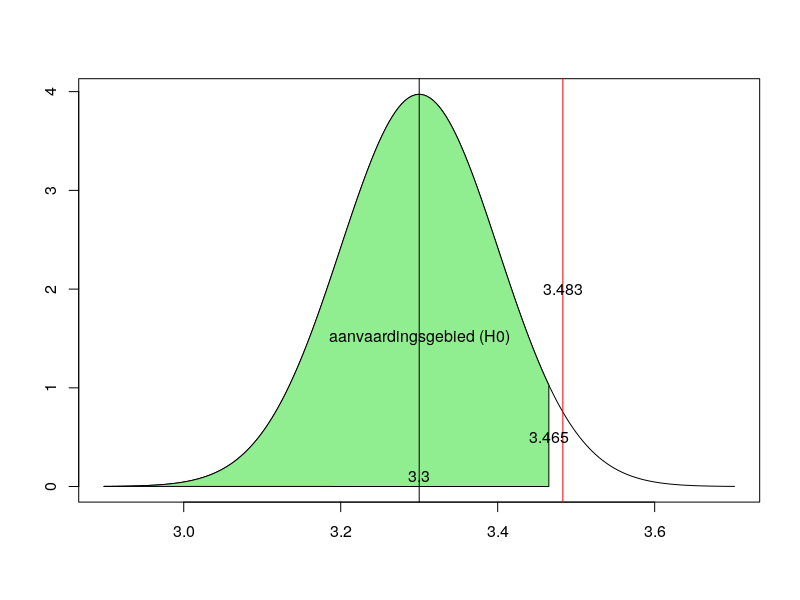
\includegraphics[width=\textwidth]{z-toets-reddingen}
  \caption{Plot in R van de situatie van Voorbeeld~\ref{ex:hypothesetoets-dagelijkse-reddingen}}
\end{figure}

\section{Voorbeelden}
\label{sec:toetsingsprocedures-voorbeelden}

\begin{example}
  Bij een aselecte steekproef van 50 waarnemingen vinden we we volgende grootheden:
  \begin{itemize}
    \item $\overline{x} = 25$
    \item $s = \sqrt{55} = 7,41$
  \end{itemize}
  
  We willen weten of er reden is om aan te nemen dat $\mu$ van de populatie kleiner is dan 27.
  
  \begin{enumerate}
    \item Bepalen van de hypothesen: 
    
    $H_{0} : \mu = 27$ en $H_{1}: \mu < 27$.
    
    \item Vastleggen significantieniveau $\alpha$ en steekproefomvang $n$:
    
    $\alpha = 0,05$ en $n=50$.
    
    \item Waarde toetsingsgrootheid bepalen. 
    
    We kiezen hiervoor het steekproefgemiddelde $M$. Volgens de centrale limietstelling geldt:
    
    \[ M \sim Nor(\mu = 27, \frac{\sigma}{\sqrt{n}}) \]
    De toetsingsgrootheid is
    \[ Z = \frac{\overline{x} - \mu}{\frac{\sigma}{\sqrt{n}}} = \frac{25-27}{\sqrt\frac{55}{50}} \approx -1,91\]
    
    \item Overschrijdingskans berekenen.
    
    We vinden een overschrijdingskans van het gemiddelde van \texttt{pnorm(-1.91)} of ongeveer $0,0281$. Bij een significantieniveau van 0,05 duidt dit er op dat we $H_{0}$ mogen verwerpen.
    
    \item Bereken en teken kritiek gebied.
    
    \[ g = \mu - z \times \frac{\sigma}{\sqrt{n}} \]
    en dus
    
    \[ g = 27 - 1,645 \times \sqrt{\frac{55}{50}} \]
    \[ g =  25,27470944 \]
    
    We vinden dus dat $\overline{x} < g$ komen tot hetzelfde besluit, nl.~dat we $H_{0}$ kunnen verwerpen.
    
  \end{enumerate}
\end{example}

\begin{example}
  In een onderzoek naar het kleingeld dat in de zakken van van onze superhelden zit, stellen de onderzoekers dat zij gemiddeld 25 euro op zak hebben. Ze gaan ervan uit de spreiding $\sigma = 7$ is. Verder zijn de gegevens van de aselecte steekproef van omvang $n=64$ beschikbaar met gemiddeld zakgeld $\overline{x}$ van 23 euro. Voor het significantieniveau kiezen ze $\alpha = 0,05$.
  
  \begin{enumerate}
    \item Bepalen van de hypothesen.
    
    $H_{0} : \mu = 25$ en $H_{1}: \mu \neq 25$.
    
    \item Vastleggen significantieniveau $\alpha$ en steekproefomvang $n$.
    
    $\alpha = 0,05$ en $n=64$.
    
    \item Bepalen van de kritieke grenzen.
    
    \[ g_{1} = \mu - z \times \frac{\sigma}{\sqrt{n}} = 23,28 \]
    
    \[ g_{2} = \mu + z \times \frac{\sigma}{\sqrt{n}} = 26,72 \]
    
    \item Kritiek gebied.
    
    We vinden dat $\overline{x}$ in het kritieke gebied ligt (want $\overline{x} = 23 < g_1 = 23,28$), dus mogen we $H_{0}$ verwerpen.
    
  \end{enumerate}
\end{example}

\section{De \texorpdfstring{$t$}{t}-toets}
\label{sec:t-toets}

Bij de $z$-toets gaan we uit van een aantal veronderstellingen waar we rekening moeten mee houden:

\begin{itemize}
  \item De steekproef moet voldoende groot zijn ($n \ge 30$);
  \item De variatie van de toetsingsgrootheid moet normaal verdeeld zijn;
  \item We veronderstellen dat de standaardafwijking van de populatie, $\sigma$, gekend is.
\end{itemize}

De eerste drie voorwaarden maken dat de centrale limietstelling kan toegepast worden.

Soms zijn deze veronderstellingen niet geldig en mogen we dan ook de $z$-toets \emph{niet} gebruiken! In deze gevallen kunnen we wel gebruik maken van de Student-$t$ verdeling. In de $t$-toets\index{$t$-toets}\index{toets!$t$-} wordt er wel van uit gegaan dat de onderzochte variabele normaal verdeeld is.

De Student-$t$ verdeling dankt zijn naam aan statisticus William Sealy Gosset\index{Gosset, William Sealy}. Hij werkte in de Guinness-brouwerij en gebruikte statistische methoden om de kwaliteit van het bier te garanderen. Zijn werkgever beschouwde dit als een bedrijfsgeheim en stond Gosset niet toe om te publiceren onder zijn eigen naam. Daarom gebruikte hij het pseudoniem Student\index{Student}.

De formule voor de kritieke grenswaarde bij de $t$-toets aangepast naar:

\begin{equation}
g = \mu \pm t \times \frac{s}{\sqrt{n}}
\label{eq:kritieke-waarde-t-toets}
\end{equation}

Voor het bepalen van de $t$-waarde hebben we het aantal vrijheidsgraden nodig, $n-1$. Om de standaardafwijking te schatten, gebruiken we de steekproefstandaardafwijking, $s$.

\begin{example}
  \label{ex:t-toets-dagelijkse-reddingen}
  Stel dat de onderzoekers van de superhelden uit Voorbeeld~\ref{ex:hypothesetoets-dagelijkse-reddingen} door tijdsdruk niet in staat waren om een voldoende grote steekproef te nemen en slechts $n = 25$ observaties gedaan hebben, met hetzelfde steekproefgemiddelde $\overline{x} = 3,483$. De standaardafwijking in deze steekproef bleek $s = 0,55$.
  
  Kunnen we in deze omstandigheden, met eenzelfde significantieniveau $\alpha = 0,05$, het besluit dat superhelden dagelijks \emph{meer} dan 3,3 mensen redden aanhouden?
  
  \begin{enumerate}
    \item Bepalen van de hypothesen.
    
      $H_{0} : \mu = 3,3$ en $H_{1}: \mu > 3,3$.
    
    \item Vastleggen significantieniveau $\alpha$ en steekproefomvang $n$.
    
    $\alpha = 0,05$ en $n=25$.
    
    \item Bepalen van de kritieke grenswaarde.
    
    \[ g_{2} = \mu + t \times \frac{s}{\sqrt{n}} \approx 3,3 + 1,711 \times \frac{0,55}{\sqrt{25}} \approx 3.488 \]
    
    De waarde voor $t$ wordt in R berekend met \texttt{qt(1-a, df = n - 1)} (met \texttt{a} het significantieniveau en \texttt{df} het aantal vrijheidsgraden.)
    
    \item Conclusie.
    
    We vinden dat $\overline{x} = 3,483$ kleiner is dan de kritieke grenswaarde en dus in het aanvaardingsgebied ligt. Met andere woorden, we mogen $H_{0}$ \emph{niet} verwerpen.
  \end{enumerate}

  Met andere woorden, ook al krijgen we gelijkaardige resultaten in onze steekproef, kunnen we niet hetzelfde besluit trekken. Omdat onze steekproef te klein is, is er grotere onzekerheid of de waarde van het steekproefgemiddelde extreem genoeg is om de nulhypothese te verwerpen.
  
  Hieronder vind je de uitwerking van dit voorbeeld in R.
\end{example}

\lstinputlisting{data/t-toets.R}

\begin{figure}
  \centering
  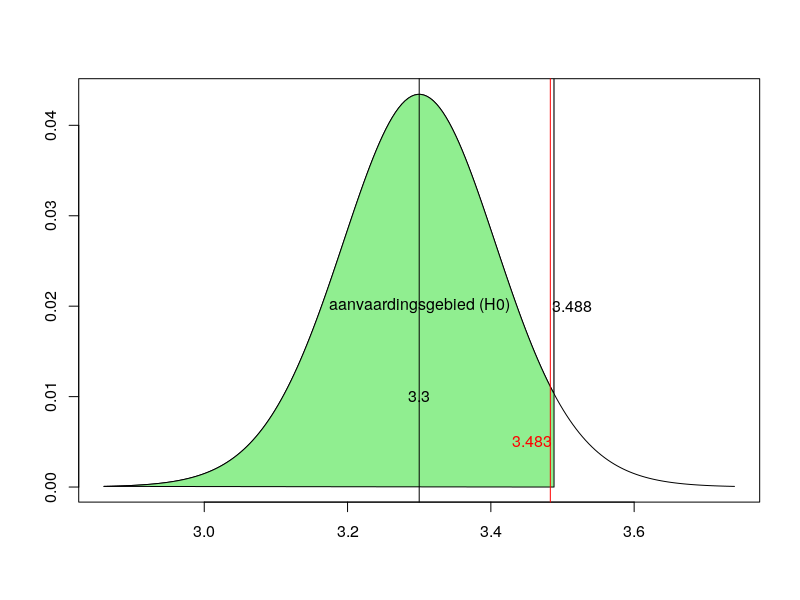
\includegraphics[width=\textwidth]{t-toets-reddingen}
  \caption{Plot in R van de situatie van Voorbeeld~\ref{ex:t-toets-dagelijkse-reddingen}}
\end{figure}

\begin{example}
  Een uitbraak van een door Salmonella veroorzaakte ziekte werd toegeschreven aan vanille-ijs van een bepaalde fabriek~\autocite{Lindquist}. Wetenschappers hebben het niveau van Salmonella gemeten in 9 willekeurig genomen steekproeven.
  
  De niveaus (in MPN/g\footnote{Most Probable Number. Zie bv.~\url{http://www.microbiologie.info/mpn-methode.html} voor meer uitleg over deze methode.}) zijn de volgende:
  
    \begin{center}
    \begin{tabular}{|l|l|l|l|l|}
      \hline
      0,593 & 0,142 & 0,329 & 0,691 & 0,231 \\ \hline
      0,793 & 0,519 & 0,392 & 0,418 &       \\ \hline
    \end{tabular}
  \end{center}

  Is er reden om aan te nemen dat het Salmonella-niveau in het ijs significant groter is dan 0,3 MPN/g? We zullen gebruik maken van de R-functie \texttt{t.test} om deze vraag te beantwoorden. Lees zelf de help-pagina van deze functie om de mogelijke opties te leren kennen.
  
  \begin{enumerate}
    \item Bepalen van de hypothesen
    
    $H_0: \mu = 0.3, H_1: \mu > 0,3$
    
    \item Vastleggen significantieniveau $\alpha = 0.05$ (in R moet je het betrouwbaarheidsniveau $1-\alpha$ opgeven, dus 0,95) en steekproefomvang $n = 9$
    
    \item Bepalen overschrijdingskans. Het gaat hier over een rechtszijdige toets, wat aangegeven wordt met de optie \texttt{alternative="greater"}. Het gekozen betrouwbaarheidsniveau is de standaardwaarde voor deze functie en moet niet expliciet meegegeven worden.
    
\begin{lstlisting}
x <- c(0.593, 0.142, 0.329, 0.691, 0.231, 0.793, 0.519, 0.392, 0.418)
t.test(x, alternative = "greater", mu = 0.3)
\end{lstlisting}
    
    Het resultaat is:
    
\begin{verbatim}
One Sample t-test

data:  x
t = 2.2051, df = 8, p-value = 0.02927
alternative hypothesis: true mean is greater than 0.3
95 percent confidence interval:
0.3245133       Inf
sample estimates:
mean of x 
0.4564444 
\end{verbatim}
    \item Conclusie. De overschrijdingskans $p = 0,029 < \alpha = 0,05$. We kunnen dus de nulhypothese verwerpen; er is met ander worden en vrij sterke aanwijzing dat het gemiddelde Salmonella-niveau in het ijs groter is dan 0,3 MPN/g.
  \end{enumerate}
\textbf{Opmerking}: \texttt{``confidence interval: 0.3245133 Inf''} heeft niet rechtstreeks met het
aanvaardingsgebied of het kritieke gebied te maken.
Het staat ook los van de waarde $\mu_{0}=0,3$.
Het zegt enkel dat vermits $\overline{x}=0,45644$,
dat we met 95\% procent zekerheid kunnen zeggen dat het \textit{\'echte} gemiddelde ($\mu$) van de populatie
tussen $0,3245133$ en $+\infty$ ligt.
Zie paragraaf \ref{ssec:betrouwbaarheidsinterval-grote-steekproef} (p. \pageref{ssec:betrouwbaarheidsinterval-grote-steekproef})
en \ref{ssec:betrouwbaarheidsinterval-kleine-steekproef} (p. \pageref{ssec:betrouwbaarheidsinterval-kleine-steekproef})
over betrouwbaarheidsintervallen.
\end{example}


\section{Fouten in hypothesetoetsen}

Bij het uitvoeren van een hypothesetoets kunnen altijd nog fouten optreden. Indien we $H_{0}$ verwerpen wanneer ze in werkelijkheid juist is, spreken we van een fout van type I en wanneer we $H_{0}$ ten onrechte aanvaarden van een fout van type II.

Het significatieniveau $\alpha$ bepaalt bij het uitvoeren van een hypothesetoets wanneer de nulhypothese precies verworpen kan worden. Stel dat we een significatieniveau van 5\% kiezen. Als de nulhypothese waar is, dan is de kans dat we een steekproef trekken met een toetsingswaarde die in het verwerpingsgebied terecht komt 5\%. M.a.w. de kans om de nulhypothese te verwerpen terwijl ze waar is, is 5 \% of in het algemeen: het significantieniveau van een toets is gelijk aan de kans op het maken van een fout van type I.

Het is vanzelfsprekend dat we de kans op een fout van type I zo klein mogelijk willen houden. Jammer genoeg is dit ten koste van de kans op een type II fout, aangeduid met $\beta$, die hierdoor groter wordt. Het verband tussen $\alpha$ en $\beta$ is niet triviaal en we gaan hier in deze cursus niet verder op in.

In vele gevallen is het maken van een fout van type I erger dan een van type II. Denk maar aan een rechtszaak waarbij de nulhypothese is dat de persoon onschuldig is. Indien we toetsen op een 5\% significantieniveau is de kans op een type I fout 5 op 100. M.a.w. er is een betrouwbaarheid van 95\% dat de juiste beslissing wordt genomen indien $H_{0}$ correct is. Daarom vermijden we liever de conclusie dat $H_{0}$ geaccepteerd wordt, maar eerder dat de steekproef onvoldoende bewijs bevat om $H_{0}$ bij een bepaald significantieniveau te verwerpen.

\begin{table}
  \centering
  \begin{tabular}{@{}l|cc@{}}
    \toprule
    & \multicolumn{2}{c}{\textbf{Werkelijke stand van zaken}} \\
    \textbf{Conclusies}          & \textbf{$H_{0}$ correct} & \textbf{$H_{1}$ correct}     \\
    \midrule
    \textbf{$H_{0}$ geaccepteerd}& Juist                    & Fout van type II \\
    \textbf{$H_{0}$ verworpen}   & Fout van type I          & Juist            \\
    \bottomrule
  \end{tabular}
  \caption{Conclusies en consequenties bij toetsen van een hypothese; types van fouten.}
  \label{tab:hypfouten}
\end{table}

\section{Oefeningen}
\label{sec:toetsingsprocedures-oefeningen}

Datasets voor deze oefeningen zijn te vinden in de Github repo, onder \texttt{oefeningen/datasets/}.



\begin{exercise}
  \label{oef:bindend-studieadvies}
  
  Er wordt gezegd dat het invoeren van een bindend studieadvies (BSA) een rendementsverhoging tot gevolg heeft in slaagkans. Voor het invoeren van het BSA was in de studentenpopulatie het gemiddelde aantal behaalde studiepunten per jaar per student gelijk aan 44 met een standaardafwijking van 6,2. Na invoering van het BSA wijst een onderzoek uit onder 72 studenten dat deze een gemiddeld aantal studiepunten haalden van 46,2.
  
  \begin{enumerate}
    \item Toets of er bewijs is dat het invoeren van een BSA leidt tot een rendementsverhoging. Gebruik methode van kritieke grenswaarde. ($\sigma = 6,2, \alpha = 2,5\%$).
    \item Toon hetzelfde aan met de methode van de overschrijdingskans.
    \item Geef een interpretatie wat de betekenis is van $\alpha = 2,5 \%$.
  \end{enumerate}
\end{exercise}

\begin{exercise}
  \label{oef:prijsverschil-autos}
  
  Eén van de motieven voor het kiezen van een garage is de inruilprijs voor de oude auto. De importeur van Ford wil graag dat de verschillende dealers een gelijk prijsbeleid voeren. De importeur vindt dat het gemiddelde prijsverschil tussen de dichtstbijzijnde Ford-dealer en de dealer waar men de auto gekocht heeft hoogstens \euro{300} mag bedragen. De veronderstelling is dat als het verschil groter is, potentiële klanten eerder geneigd zullen zijn om bij hun vorige dealer te blijven.
  
  In een steekproef worden volgende verschillen genoteerd:
  
  \begin{center}
    \begin{tabular}{|l|l|l|l|l|l|l|}
      \hline
      400 & 350 & 400 & 500 & 300 & 350 & 200 \\ \hline
      500 & 200 & 250 & 250 & 500 & 350 & 100 \\ \hline
    \end{tabular}
  \end{center}

  Toets of er reden is om aan te nemen dat het gemiddelde prijsverschil in werkelijkheid significant groter is dan \euro{300}. Gebruik een significantieniveau van 5\%. 
  
\end{exercise}

\begin{exercise}
  \label{ex:z-toets-rlanders}
  Lees de dataset \texttt{rlanders-generated.csv} in\footnote{Deze dataset bevat synthetische data, gegenereerd met hulp van \url{https://rlanders.net/dataset-generator/}}.
  
  De variabele \emph{Money} stelt een bruto-jaarsalaris voor ($\times 100\$$). We gaan er van uit dat het deze variabele een gemiddelde $\mu = 490$ heeft en standaardafwijking $\sigma = 98$. Als we het steekproefgemiddelde berekenen over de gehele dataset (doe dit zelf!), lijkt dat de veronderstelling te ondersteunen. Maar wat als we naar de mannen en de vrouwen afzonderlijk zouden kijken (variabele \emph{Gender})?
  
  Gebruik een geschikte statistische toets om de uitspraken hieronder te verifiëren. Gebruik daarbij significantieniveau $\alpha = 5\%$. Bereken telkens de kritieke grenswaarde(n) en de p-waarde.
  
  \begin{enumerate}
    \item Het gemiddelde jaarsalaris van de mannen lijkt hoger dan de verwachte waarde. Is het ook significant hoger?
    \item Het gemiddelde jaarsalaris van de vrouwen lijkt \emph{lager}. Is het ook significant lager?
    \item Bepaal tenslotte het aanvaardingsgebied voor het gemiddelde jaarsalaris over de gehele steekproef (vrouwen en mannen samen) als we zouden willen bepalen of het steekproefgemiddelde significant afwijkt van de verwachte waarde, zonder een uitspraak te doen of die al dan niet hoger of lager ligt.
  \end{enumerate}
  
\end{exercise}

\section{Antwoorden op geselecteerde oefeningen}
\label{sec:toetsingsprocedures-antwoorden}

\paragraph{Oefening~\ref{ex:kritieke-waarde-linkszijdig}:}

\begin{equation}
g = \mu - z \times \frac{\sigma}{\sqrt{n}}
\label{eq:kritiekeRechtseWaarde2}
\end{equation}

want

\[ P(M < g) = P\left(Z < \frac{g - \mu}{\frac{\sigma}{\sqrt{n}}}\right) = 0,05 \]
Wegens de symmetrieregel kunnen we zeggen
\[ P\left(Z > - \left( \frac{g - \mu}{\frac{\sigma}{\sqrt{n}}} \right) \right) = 0,05 \]
De z-waarde die ermee overeen komt is 1,645 dus hebben we
\[ z = \frac{-g + \mu}{\frac{\sigma}{\sqrt{n}}} \]
\[ \Leftrightarrow -g = \frac{\sigma}{\sqrt{n}} z - \mu \]
\[ \Leftrightarrow g = -\frac{\sigma}{\sqrt{n}} z + \mu \]

\paragraph{Oefening~\ref{oef:bindend-studieadvies}}

\begin{enumerate}
  \item $g \approx 45,4 < \overline{x} = 46,2$.
  
  $\overline{x}$ ligt in het kritieke gebied, dus we mogen de nulhypothese verwerpen. We hebben dus redenen om aan te nemen dat bindend studieadvies inderdaad het studierendement significant verhoogt.
  
  \item $P(M > 46.2) \approx 0,0013 < \alpha = 0,025$. De overschrijdingskans is kleiner dan het significantieniveau, dus we mogen de nulhypothese verwerpen.
  
  \item  $\alpha$ is de kans dat je $H_{0}$ ten onrechte verwerpt. Er is m.a.w.~een kans van 2,5\% dat je ten onrechte de conclusie trekt dat het studierendement hoger is geworden.
\end{enumerate}

\paragraph{Oefening~\ref{oef:prijsverschil-autos}}

In deze situatie ($n = 14 < 30$) mogen we geen $z$-toets gebruiken, maar vallen we terug op de $t$-toets.

\begin{itemize}
  \item $\overline{x} \approx 332,143$
  \item $s \approx 123,424$
  \item $g \approx 358,42$. Het steekproefgemiddelde ligt niet in het kritieke gebied, dus we kunnen $H_0$ \emph{niet} verwerpen.
  \item $p \approx 0,1738$. $p \nless \alpha$, dus we kunnen $H_0$ \emph{niet} verwerpen.
\end{itemize}

Er is op basis van deze steekproef dus geen reden om aan te nemen dat het gemiddelde prijsverschil op de inruilprijs van oude wagens significant groter is dan door de importeur aanbevolen.

\paragraph{Oefening \ref{ex:z-toets-rlanders}}

Het gemiddelde van de hele steekproef is $\overline{x} \approx 501,156$

\begin{enumerate}
  \item Voor de mannen (rechtszijdige $z$-toets):
    \begin{itemize}
      \item $\overline{x}_m \approx 507,535$
      \item $g_m \approx 511,456$
      \item $p_m \approx 0,1396$
      \item We mogen de nulhypothese \textit{niet} verwerpen. Het bruto jaarsalaris van de mannen in de steekproef is niet significant hoger dan verwacht.
    \end{itemize}
  \item Voor de vrouwen (linkszijdige $z$-toets):
    \begin{itemize}
      \item $\overline{x}_f \approx 472,058$
      \item $g_f \approx 477,646$
      \item $p_f \approx 0,0199$
      \item We mogen de nulhypothese verwerpen. Het bruto jaarsalaris van de vrouwen in de steekproef is significant lager dan verwacht.
    \end{itemize}
  \item Het aanvaardingsgebied is het interval [487,852; 512,148]. 
\end{enumerate}

\chapter{Bivariate analyse}
\label{ch:analyse2var}

In de vorige hoofdstukken hebben we telkens één variabele tegelijkertijd onderzocht. In dit hoofdstuk bestuderen we \emph{verbanden}\index{verband} (ook: \emph{samenhang}\index{samenhang} of \emph{associatie}\index{associatie}) tussen variabelen. We spreken van een verband tussen twee variabelen wanneer de waarde van de ene variabele op een systematische manier verandert ten opzichte van de waarde van de andere. Anders gezegd, wanneer we tot op zekere hoogte een voorspelling kunnen doen over de waarde van een variabele aan de hand van de waarde van een andere.

\section{Leerdoelen}
\label{sec:analyse2var-leerdoelen}

Na dit hoofdstuk moet je in staat zijn om:

\begin{itemize}
  \item De volgende begrippen uit dit hoofdstuk uit te leggen:
  \begin{itemize}
    \item afhankelijke variabele, onafhankelijke variabele;
    \item een verband (samenhang, associatie) tussen twee variabelen, stijgend/dalend verband, lineair verband;
  \end{itemize}
  \item Voor de in dit hoofstuk besproken combinaties van meetniveaus geschikte analysetechnieken te benoemen;
  \item Voor een combinatie van twee kwalitatieve variabelen:
  \begin{itemize}
    \item Een kruistabel op te stellen en de regel van Cochran toe te passen;
    \item De $\chi^2$-statistiek te berekenen;
    \item De $\chi^2$-toets uit te voeren (voor associatie en goodness-of-fit);
    \item Gestandaardiseerde residuën te berekenen en te interpreteren;
    \item Cramér's V te berekenen en de waarde te interpreteren
  \end{itemize}
  \item Voor een combinatie van een kwalitatieve onafhankelijke en kwantitatieve afhankelijke variabele:
  \begin{itemize}
    \item De correcte variant van de $t$-toets voor twee steekproeven (gepaard, onafhankelijk) toe te passen;
    \item De effectgrootte (Cohen's $d$) te berekenen en de waarde te interpreteren;
  \end{itemize}
  \item Voor een combinatie van twee kwantitatieve variabelen:
  \begin{itemize}
    \item het functievoorschrift van de regressierechte te bepalen en die te tekenen;
    \item de covariantie, correlatiecoëfficiënt en determinatiecoëfficiënt te berekenen en de waarde ervan met de correcte verwoordingen te interpreteren;
  \end{itemize}
  \item Voor de in dit hoofstuk besproken combinaties van meetniveaus geschikte visualisatietechnieken te benoemen en toe te passen;
  \item Een gegeven grafiek met twee variabelen te interpreteren, o.a.~het grafiektype benoemen, afleiden of er een verband bestaat, welk soort verband en de mate van associatie (zwak, matig, sterk).
  \item Aan de hand van een situatie kunnen uitleggen dat een verband niet noodzakelijk een noodzakelijk verband inhoudt, en waarom;
\end{itemize}

\section{Inleiding}
\label{sec:analyse2var-inleiding}

Wanneer we een verband beschrijven tussen variabelen, onderscheiden we:

\begin{itemize}
  \item De \emph{afhankelijke variabele}\index{variabele!afhankelijke}, waarover we een voorspelling willen doen;
  \item De \emph{onafhankelijke variabele}\index{variabele!onafhankelijke}, op basis van dewelke we de voorspelling doen.
\end{itemize}

Dus als de onafhankelijke variabele op een bepaalde manier verandert, verwachten we dat de waarde van de afhankelijke variabele op een voorspelbare manier mee verandert.

\begin{example}
  Een voorbeeld waarbij verbanden kunnen gevonden worden tussen variabelen vind je bij Ant Colony Optimization (ACO). Dit is een techniek die gebruikt wordt in verschillende computationele problemen. Men baseert zich hier op hoe mieren voedsel zoeken en  vinden en dat communiceren aan de groep. Mieren verspreiden feromonen als ze op pad gaan op zoek naar eten. Hoe langer het pad, hoe minder feromonen het pad zal bevatten, hoe korter het pad, hoe groter de kans dat er een grote concentratie aan feromonen te vinden is. Mieren worden aangetrokken door deze feromonen en zullen dus proberen de meest bewandelde paden te gebruiken om naar een bepaalde voedselbron te gaan. Nu kan je onderzoeken of de tijd voor het vinden van een pad, afhangt van een aantal variabelen:

  \begin{itemize}
    \item De mate waarin feromonen verspreid worden
    \item De mate waarin een feromoon verdwijnt
    \item Het aantal obstakels tussen het nest en de voedselbron
    \item De vorm van de obstakels tussen nest en voedselbron (vinden ze sneller het pad indien er geen hoeken aan de obstakels zijn bv.)
  \end{itemize}
\end{example}

Voor het onderzoeken of er een verband bestaat tussen twee variabelen bestaan er verschillende analyse- en visualisatietechnieken die afhangen van het meetniveau. Tabel~\ref{tab:analyse2var} geeft een overzicht van geschikte analysetechnieken die in deze cursus besproken worden en Tabel~\ref{tab:visualisatie2var} van geschikte grafiektypes.

Merk trouwens op dat er nog veel meer analysetechnieken bestaan die niet in deze cursus besproken worden! Hier vind je enkel een topje van de ijsberg\ldots Als je in je latere carrière nood hebt aan statistische technieken (en de auteurs van deze cursus zijn optimistisch dat dit ook effectief ooit eens zal gebeuren), kijk je best na of er betere technieken bestaan voor het beantwoorden van jouw specifieke onderzoeksvraag.

\begin{table}
  \begin{tabular}{llll}
    \toprule
    \textbf{Onafhankelijke} & \textbf{Afhankelijke} & \textbf{Toets}                & \textbf{Metriek}      \\
    \midrule
    Kwalitatief             & Kwalitatief           & $\chi^2$-toets                & Cramér's $V$          \\
    Kwalitatief             & Kwantitatief          & $t$-toets voor 2 steekproeven & Cohen's $d$           \\
    Kwantitatief            & Kwantitatief          & ---                           & Regressie, correlatie \\
    \bottomrule
  \end{tabular}
  \caption{Overzicht van analysetechnieken voor het verband tussen twee variabelen. De tabel geeft telkens enerzijds geschikte statistische toetsen en anderzijds metrieken die de mate van het verband uitdrukken.}
  \label{tab:analyse2var}
\end{table}

\begin{table}
  \begin{tabular}{lll}
  	\toprule
  	\textbf{Onafhankelijke} & \textbf{Afhankelijke} & \textbf{Grafiektype}                                  \\
  	\midrule
  	Kwalitatief             & Kwalitatief           & Mozaïekdiagram, rependiagram, geclusterd staafdiagram \\
  	Kwalitatief             & Kwantitatief          & Boxplot, staafdiagram met error bars                  \\
  	Kwantitatief            & Kwantitatief          & Spreidingsdiagram, regressierechte                    \\
  	\bottomrule
  \end{tabular}
  \caption{Overzicht van visualisatietechnieken voor het verband tussen twee variabelen.}
  \label{tab:visualisatie2var}
\end{table}

\section{Kwalitatief--kwalitatief}
\label{sec:kwalitatief-kwalitatief}

In deze sectie bekijken we methoden om na te gaan of er een verband bestaat tussen twee kwalitatieve variabelen. Al deze methoden zijn gebaseerd op een samenvattende tabel van frequenties van de twee variabelen, de kruistabel (zie Sectie~\ref{ssec:kruistabellen}). Daaruit wordt een statistiek berekend die uitdrukt hoe groot de verschillen zijn tussen de twee variabelen, de zogenaamde ``Chi-kwadraat'', notatie $\chi^2$\footnote{Chi, $\chi$ is een letter uit het Griekse alfabet.} (zie Sectie~\ref{ssec:chi-kwadraat}). Met de $\chi^2$-toets (zie Sectie~\ref{ssec:onafhankelijkheidstoets} en~\ref{ssec:aanpassingstoets}) kan je nagaan of de waarde van $\chi^2$ al dan niet aangeeft of er een verband bestaat tussen twee variabelen. Er bestaat ook een metriek, Cramér's $V$ (zie Sectie~\ref{ssec:cramers-v}), die de waarde van $\chi^2$ herleidt tot een getal tussen 0 en 1 waaruit de sterkte van het verband valt af te leiden.

\subsection{Kruistabellen}
\label{ssec:kruistabellen}

\begin{definition}[Kruistabel]
  In een kruistabel\index{kruistabel} (Eng.: \emph{contingency table} of \emph{cross table}; zie bv.~Figuur~\ref{tab:kruistabel0}) worden de frequenties van twee variabelen samengevat.
  
  Elke cel van de laatste kolom bevat de som van de overeenkomstige rij en elke cel van de laatste rij bevat de som van de overeenkomstige kolom. Dit worden de \emph{marginale totalen}\index{totaal!marginaal}\index{marginaal totaal} genoemd.
\end{definition}

\begin{table} \centering
  \begin{tabular}{@{}rrrr}
    \toprule
                & Vrouw & Man & Totaal \\
    \midrule
           Goed &     9 &   8 &     17 \\
      Voldoende &     8 &  10 &     18 \\
    Onvoldoende &     5 &   5 &     10 \\
         Slecht &     0 &   4 &      4 \\
         Totaal &    22 &  27 &     49 \\
    \bottomrule
  \end{tabular}
  \caption{Een kruistabel voor de waardering door mannen en vrouwen van een bepaald assortiment producten.}
  \label{tab:kruistabel0}
\end{table}

Hoe kunnen we nu zien in een kruistabel of er een verband bestaat tussen twee variabelen? Bekijk de kruistabel in Tabel~\ref{tab:kruistabel0}. Die geeft de resultaten weer van een bevraging waar 49 mensen (22 vrouwen en 27 mannen) gevraagd werd om een waardering te geven (goed, voldoende, onvoldoende of slecht). Als er een verband bestaat tussen de twee variabelen, gender (onafhankelijk) en waardering (afhankelijk), dan moeten we zien dat vrouwen en mannen fundamenteel andere waarderingen gegeven hebben. Omgekeerd, als zowel bij de vrouwen als bij de mannen de verhoudingen tussen de verschillende waarderingen (ongeveer) gelijk zijn, dan is er \emph{geen} verband.

In een gewone kruistabel kunnen we geen directe conclusies trekken, aangezien het analyseren of er samenhang bestaat tussen variabelen niet goed gaat op basis van de absolute frequenties. Er zijn immers meer mannen dan vrouwen in de bevraging! Daarom moeten we percenteren, d.w.z.~binnen elke kolom het percentage berekenen hoe vaak elke beoordeling \emph{naar verhouding} voorkomt. De som van alle percentages in een kolom moet dan gelijk zijn aan 100\%. Nog even snel de regel van percenteren:

\begin{itemize}
  \item Om te weten hoeveel procent $x$ is van $y$, deel je $x$ door $y$ en vermenigvuldig je met 100: $p = \frac{x}{y} \times 100$. Bijvoorbeeld: hoeveel procent is 15 van 20? $\frac{15}{20} \times 100 = 75$, dus 75\%.
  \item Om te weten hoeveel $x\%$ is van $y$: $\frac{x \times y}{100}$. Hoeveel is 60\% van 30? $\frac{60 \times 30}{100} = 18$.
\end{itemize}

In Tabel~\ref{tab:kruistabel1} vind je per geslacht de percentages dat elke waardering is voorgekomen in de steekproef. We zien dan bijvoorbeeld dat 41\% van de vrouwen een waardering goed heeft gegeven (want 9 is ongeveer 41\% van 22), tegen dat 30\% van de mannen.

\begin{table} \centering
  \begin{tabular}{@{}rrrrrrr@{}}
  	\toprule
  	            & Vrouw & Man & Totaal & Vrouw \% & Man\% & Totaal \\
  	\midrule
  	       Goed &     9 &   8 &     17 &     41\% &  30\% &   35\% \\
  	  Voldoende &     8 &  10 &     18 &     36\% &  37\% &   37\% \\
  	Onvoldoende &     5 &   5 &     10 &     23\% &  18\% &   20\% \\
  	     Slecht &     0 &   4 &      4 &      0\% &  15\% &    8\% \\
  	     Totaal &    22 &  27 &     49 &    100\% & 100\% &  100\% \\
  	\bottomrule
  \end{tabular}
  \caption{De kruistabel waarbij we de waarden gepercenteerd hebben.}
  \label{tab:kruistabel1}
\end{table}

Nu kunnen we ons de vraag stellen of de waarderingskeuze afhangt van het gender van de respondent. Er zijn verschillen tussen beide kolommen, dus je kan een vermoeden hebben dat dit inderdaad het geval is. Hoe kleiner de verschillen, hoe minder verband er is tussen beide variabelen, hoe groter de verschillen, hoe groter de samenhang.

\subsection{\texorpdfstring{$\chi^{2}$}{chi-kwadraat}}
\label{ssec:chi-kwadraat}

Uit de vorige sectie kunnen we besluiten dat we nood hebben aan een maat die uitdrukt hoe groot het verschil is tussen de verhoudingen in beide kolommen. Een manier om dit uit te drukken wordt de \emph{chi-kwadraat}-statistiek (notatie $\chi^{2}$) genoemd. $\chi^2$ is gelijk aan 0 als er geen verschil is tussen de verhoudingen in de kolommen van een kruistabel, en als er dus ook volstrekt geen samenhang tussen de variabelen is. Als er wel een verschil is, dan is $\chi^2$ een positief getal. Hoe groter de waarde, hoe groter ook de onderlinge verschillen tussen de kolommen en hoe groter dus ook de samenhang.

De procedure om de $\chi^2$ van een kruistabel te berekenen gaat als volgt:

\begin{enumerate}
  \item Stel eerst de kruistabel op samen met marginale totalen (zie tabel \ref{tab:kruistabel0}).
  \item Vervolgens berekenen we voor elke cel de zogenaamde \emph{verwachte frequentie} (notatie $e$ van \emph{expected}). Dat is de absolute frequentie die je in deze cel zou \emph{verwachten} als je veronderstelt dat er helemaal geen samenhang is tussen de variabelen. Deze kan je bereken als volgt:
  
  \begin{equation}
  e = \frac{rijtotaal \times kolomtotaal}{n}
  \end{equation}
  
  met:
  
  \begin{itemize}
    \item $rijtotaal$ totaal van de rij van de betreffende cel
    \item $kolomtotaal$ totaal van de kolom van de betreffende cel
    \item $n$ het aantal observaties
  \end{itemize}
  
  Voor cel$_{1,2}$ (het verwachte aantal mannen dat waardering ``goed'' gegeven heeft) is dit dus $\frac{17 \times 27}{49} \approx 9.37\%$.
  
  \item Dan bereken je het verschil tussen geobserveerde (notatie $o$, \emph{observed}) en verwachte frequentie ($e$). (Zie tabel~\ref{tab:kruistabel2}).
  
  \begin{table} \centering
    \begin{tabular}{@{}rrrrrrr@{}}
    	\toprule
    	            &                       Vrouw &                          Man & Totaal & Vrouw \% &   Man\% &  Totaal \\
    	\midrule
    	       Goed &  $9 -\textcolor{red}{7.63}$ &  $8 - \textcolor{red}{9.36}$ &   $17$ &   $41$\% &  $30$\% &  $35$\% \\
    	  Voldoende & $8 - \textcolor{red}{8.08}$ & $10 - \textcolor{red}{9.91}$ &   $18$ &   $36$\% &  $37$\% &  $37$\% \\
    	Onvoldoende & $5 - \textcolor{red}{4.48}$ &  $5 - \textcolor{red}{5.51}$ &   $10$ &   $23$\% &  $18$\% &  $20$\% \\
    	     Slecht & $0 - \textcolor{red}{1.79}$ &  $4 - \textcolor{red}{2.20}$ &    $4$ &    $0$\% &  $15$\% &   $8$\% \\
    	     Totaal &                        $22$ &                         $27$ &   $49$ &  $100$\% & $100$\% & $100$\% \\
    	\bottomrule
    \end{tabular}
    \caption{De kruistabel waarbij we de verwachte frequentie $e$ (aangeduid in het rood) bepaald hebben voor elke cel en die aftrekken van de geobserveerde frequentie $o$.}
    \label{tab:kruistabel2}
  \end{table}
  
  \item De laatste stap houdt in dat we een berekening gaan maken voor de maat van afwijking voor elke cel. Net zoals bij het berekenen van de variantie van een steekproef (zie Sectie~\ref{sec:varEnSD}) kwadrateren we het verschil zodat het resultaat altijd positief is en zodat grotere afwijkingen zwaarder door zullen wegen in het resultaat.
  
  We gaan ook de afwijking delen door de verwachte frequentie om hen relatief even belangrijk te maken. Bijvoorbeeld: een afwijking van 5 op een verwachte frequentie van 20 is groter dan bv. een afwijking op een verwachte frequentie van 200. Dit geeft dan voor elke cel van de kruistabel de volgende berekening (zie Tabel~\ref{tab:kruistabel3}):
  
  \begin{equation}
  \frac{(o - e)^{2}}{e}
  \end{equation}
  
  \begin{table} \centering
    \begin{tabular}{@{}rrrrrrr@{}}
    	\toprule
    	            &                    Vrouw &                      Man & Totaal & Vrouw \% &   Man\% &  Totaal \\
    	\midrule
    	       Goed & $\textcolor{blue}{0.24}$ & $\textcolor{blue}{0.20}$ &   $17$ &   $41$\% &  $30$\% &  $35$\% \\
    	  Voldoende & $\textcolor{blue}{0.00}$ & $\textcolor{blue}{0.00}$ &   $18$ &   $36$\% &  $37$\% &  $37$\% \\
    	Onvoldoende & $\textcolor{blue}{0.06}$ & $\textcolor{blue}{0.05}$ &   $10$ &   $23$\% &  $18$\% &  $20$\% \\
    	     Slecht & $\textcolor{blue}{1.80}$ & $\textcolor{blue}{1.46}$ &    $4$ &    $0$\% &  $15$\% &   $8$\% \\
    	     Totaal &                     $22$ &                     $27$ &   $49$ &  $100$\% & $100$\% & $100$\% \\
    	\bottomrule
    \end{tabular}
    \caption{De kruistabel waarbij we het verschil gekwadrateerd hebben en gedeeld door de verwachte frequentie, $\frac{(o - e)^2}{e}$ (in het blauw). Merk op dat deze waarden afgerond zijn tot twee cijfers na de komma, en we hier dus een deel van de precisie kwijt spelen.}
    \label{tab:kruistabel3}
  \end{table}
  
  \item Alle resultaten gaan we tenslotte optellen om zo de $\chi^{2}$ te bekomen:
  
  \begin{equation}
  \chi^{2} = \sum \frac{(o - e)^{2}}{e}
  \end{equation}
  
  In het voorbeeld is $\chi^2 \approx 3,8105$.
\end{enumerate}

Nu zegt deze waarde $\chi^2 \approx 3,8105$ op zich nog \emph{steeds} niet zo veel. Onder welke voorwaarden zeggen we dat er al dan niet een verband is tussen beide variabelen? En hoe sterk is dat verband dan? Een en ander zal ook afhangen van de grootte van de tabel en het totaal aantal observaties. In een kruistabel met meer rijen/kolommen, zal je een grotere $\chi^2$ moeten hebben om te besluiten dat er een verband is.

\subsection[Chi-kwadraatverdeling]{$\chi^{2}$ verdeling}
\label{ssec:chi-kwadraatverdeling}

In Sectie~\ref{ssec:onafhankelijkheidstoets} wordt de $\chi^2$-toets gedefinieerd. Deze toets maakt bij het bepalen van de overschrijdingskans of kritieke grenswaarde gebruik van de zgn.~$\chi^2$-verdeling. Deze stochastische verdeling komt niet in de natuur voor en geen verschijnsel kan erdoor gemodelleerd worden. In \emph{deze} context is ze echter \emph{wel} zeer nuttig.

Laat $X_{1}, X_{2}, \dots X_{v}$ onafhankelijk standaardnormale variabelen zijn ($\sim N(0,1)$). De $\chi^{2}$ (chi-kwadraat) variabele wordt als volgt gedefinieerd:

\[ \chi^{2}_{v} = X_{1}^{2} + X_{2}^{2} + \dots + X_{v}^{2} \]

Het getal $v$ noemt men het aantal vrijheidsgraden van de variabele. $\chi^{2}$ is een continue toevalsveranderlijke, die positief is omdat ze de som is van kwadraten. Haar dichtheidsfunctie is de volgende:

\[ f_{n}(x) = \frac{1}{2^{\frac{n}{2}}\Gamma(\frac{n}{2})} x^{\frac{n}{2} -1} e^{\frac{x}{2}} \]

De verwachtingswaarde (= gemiddelde) is $v$ en zijn variantie is $2v$. Zijn modus voor $v \geq 2$ is $v-2$.

Voor het bepalen van de nodige waarden binnen de $\chi^2$-verdeling (bv. rechterstaartkans, kritieke grenswaarde), kunnen we gebruik maken van hetzij een tabel\footnote{Bijvoorbeeld \url{https://people.richland.edu/james/lecture/m170/tbl-chi.html}}, hetzij statistische software zoals R.

\begin{figure}
  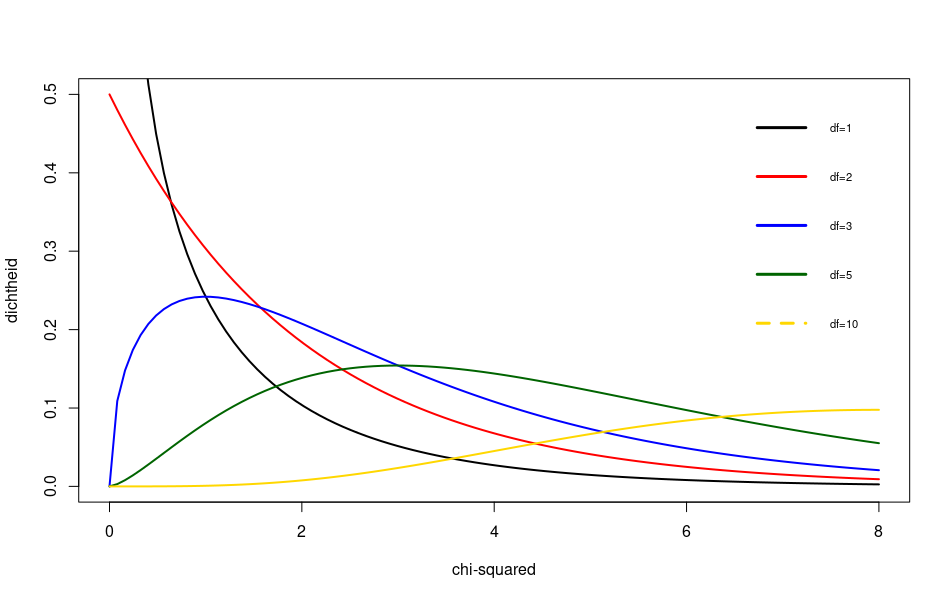
\includegraphics[width=\textwidth]{chi-squared-distribution}
  \caption{Dichtheidsfunctie van de $\chi^2$-verdeling voor verschillende vrijheidsgraden $df$.}
  \label{fig:chi-squared-distribution}
\end{figure}

\subsection{Onafhankelijkheidstoets}
\label{ssec:onafhankelijkheidstoets}

Een onafhankelijkheidstoets\index{onafhankelijkheidstoets} gaat na of er een verband bestaat tussen twee kwalitatieve variabelen aan de hand van de $\chi^2$-statistiek. Deze toets wordt ook de $\chi^2$-toets\index{$\chi^2$-toets!}\index{toets!$\chi^2$-} voor associatie genoemd, of de $\chi^2$-kruistabeltoets, en is ontwikkeld door de Engelse wiskundige en statisticus Karl Pearson\index{Pearson!Karl}.

\subsubsection{Toetsingsprocedure}

De toetsingsprocedure verloopt als volgt:

\begin{enumerate}
  \item \textbf{Bepalen hypotheses}
  Als nulhypothese stellen we dat er geen verband is tussen de onafhankelijke en de afhankelijke variabele (en verwachten we dus een kleine $\chi^2$). Als alternatieve hypothese stellen we dat er \emph{wel} een verband is (en dat $\chi^2$ dus groot is).
  \begin{itemize}
    \item $H_{0}$: er is geen verband tussen de variabelen (of: de variabelen zijn onafhankelijk)
    \item $H_{1}$: er is een verband tussen de variabelen
  \end{itemize}

  \item \textbf{Bepalen significantieniveau $\alpha$}
  
  \item \textbf{Bereken de waarde van de toetsingsgrootheid in de steekproef}
  \[ \chi^{2} = \sum_{i} \frac{(o_{i} - e_{i})^{2}}{e_{i}} \]
  
  \item De waarde van $\chi^2$ is gedistribueerd volgens de $\chi^2$-verdeling (zie Sectie~\ref{ssec:chi-kwadraatverdeling}). Deze stochastische verdeling heeft als bijkomende parameter het aantal vrijheidsgraden $df$. Voor een kruistabeltoets is $df = (r - 1) \times (k - 1)$ met $r$ het aantal rijen en $k$ het aantal kolommen.
  
  Aan de hand van deze verdeling kunnen we op twee equivalente manieren een besluit trekken:
  
  \begin{enumerate}
    \item \textbf{Bereken en teken kritiek gebied}. De kritieke grenswaarde $g$ is het getal waarvoor geldt dat $P(\chi^2 > g) = \alpha$. Deze toets is altijd rechtszijdig. Als $\chi^2 < g$, dan zitten we in het \emph{aanvaardingsgebied}, waar we de nulhypothese niet kunnen verwerpen. Als $\chi^2 > g$, dan zitten we in het \emph{verwerpingsgebied} en zullen we de nulhypothese verwerpen.
    \item \textbf{Bereken de overschrijdingskans $p$}. Dit is de rechterstaartkans voor de bekomen $\chi^2$-statistiek in de steekproef, afhankelijk van het aantal vrijheidsgraden. De interpretatie van de $p$-waarde is ``Als we zouden veronderstellen dat er \emph{geen} verband is tussen de twee variabelen, wat is dan de kans dat ik een waarde voor $\chi^2$ tegenkom in een steekproef die minstens zo groot is als de daarnet berekende?'' Als $p > \alpha$ (en dus de kans relatief groot is dat we deze $ \chi^2$-waarde tegenkomen), dan aanvaarden we de nulhypothese, als $p < \alpha$, dan verwerpen we deze.
  \end{enumerate}

  \item Tenslotte formuleren we de conclusie en beantwoorden we de onderzoeksvraag.
\end{enumerate}

Toegepast op het voorbeeld van hierboven:

\begin{enumerate}
  \item \textbf{Bepalen hypotheses:}
  \begin{itemize}
    \item $H_0$ Er is geen verband tussen gender en waardering
    \item $H_1$ Er is een verband tussen gender en waardering
  \end{itemize}
  \item \textbf{Bepalen significantieniveau:} $\alpha = 0,05$
  
  \item \textbf{Bereken de waarde van de toetsingsgrootheid in de steekproef}
  
  $\chi^2 \approx 3,8105$ (zie Sectie~\ref{ssec:chi-kwadraat})
  
  \item Bepaal het aantal vrijheidsgraden $df = (r - 1) \times (k - 1) = (4 - 1) \times (2 - 1) = 3$.
  
  \begin{enumerate}
    \item \textbf{Bepaal de kritieke grenswaarde:} $g \approx 7,815$. In dit geval is $\chi^2 < g$, dus we zitten in het aanvaardingsgebied. We kunnen $H_0$ dus niet verwerpen.
    \item \textbf{Bereken de overschrijdingskans:} $p \approx 0,2827$. Er is dus een kans van ongeveer 28\% dat we deze $\chi^2$-waarde tegenkomen. Dat is vrij groot, zeker al groter dan $\alpha$. Bijgevolg kunnen we $H_0$ niet verwerpen.
  \end{enumerate}

  \item We kunnen dus besluiten dat er op basis van deze steekproef geen reden is om aan te nemen dat er een verband is tussen gender en waardering. Anders gezegd, er zijn geen significante verschillen tussen de waarderingen bij enerzijds vrouwen en anderzijds mannen.
\end{enumerate}


We geven nog een ander voorbeeld van de onafhankelijkheidstoets aan de hand van een studie door \textcite{Doll1954} over de relatie tussen roken en longkanker. Doll en Hill schreven in 1951 alle Britse huisartsen aan met het verzoek om gegevens over hun leeftijd en rookgedrag. Vervolgens hielden ze jarenlang de overlijdensberichten en de doodsoorzaak bij en herhaalden hun periodiek. De eerste uitkomsten, na circa vier jaar, zijn in tabel~\ref{tab:dollhill} samengevat. Uit de tabel kan makkelijk geconcludeerd worden dat er geen relatie is tussen roken en longkanker. In (ruim) vier jaar is slechts $(84 / 24354) * 100 = 0,35\%$ van de Britse artsen aan longkanker overleden en dat met slechts $(83 / 21261) * 100 = 0,39\%$ van de rokers onder hen. Dit is weinig, maar het is wel veel meer dan hetzelfde cijfer voor de niet-rokers $(1 / 3093) * 100 = 0,032\%$.

\begin{table}
  \begin{center}
    \begin{tabular}{@{}lllll@{}}
    	\toprule
    	               & \textbf{Longkanker} & \textbf{Niet} & \textbf{Wel} & \textbf{Totaal} \\
    	\midrule
    	\textbf{Roker} & \textbf{Wel}        & 21178         & 83           & 21261           \\
    	               & \textbf{Niet}       & 3092          & 1            & 3093            \\
    	               & \textbf{Totaal}     & 24270         & 84           & 24354           \\
    	\bottomrule
    \end{tabular}
  \end{center}
  \caption{Resultaten van het onderzoek van~\textcite{Doll1954}}
  \label{tab:dollhill}
\end{table}

We zien in de tabel dat er wel een erg groot verschil is tussen de geobserveerde aantallen rokers die overlijden aan longkanker en de verwachte frequenties in deze cel. Hetzelfde geldt voor het geringe aantal huisartsen dat niet rookt, maar wel aan longkanker overleden is. Deze observatie maakt ons wel wantrouwig of de eerdere tentatieve conclusie wel juist is. We kunnen afrekenen met deze onzekerheid door de toetsingsgrootheid $\chi^{2}$ uit te rekenen. Dat doen we op de vertrouwde manier:

\begin{enumerate}
  \item \textbf{Bepalen hypotheses}
  \begin{itemize}
    \item $H_{0}$: er is geen verband tussen roken en sterven aan longkanker
    \item $H_{1}$: er is een verband tussen roken en sterven aan longkanker
  \end{itemize}
  \item \textbf{Bepalen $\alpha$ en $n$:} $\alpha = 0,05$ en $n = 24354$.
  \item \textbf{Toetsingsgrootheid en waarde ervan in steekproef}:
  \[ \chi^{2} = \sum_{i=1}^{k \times r} \frac{(o_{i} - e_{i})^{2}}{e_{i}} \approx 10,071 \]
  \item \textbf{Bereken en teken kritiek gebied}: Het aantal vrijheidsgraden is $df = (r-1)(k-1) = 1$, dus voor het gegeven significantieniveau is de kritieke grens 3,8415. Onze toetsingsgrootheid ligt in het kritieke gebied dus verwerpen we $H_{0}$.
\end{enumerate}

We moeten derhalve $H_{0}$, dat er geen relatie is tussen beide variabelen, verwerpen ten gunste van $H_{1}$ dat er wel een relatie is tussen beide variabelen: rokers sterven vaker aan longkanker dan niet-rokers.

Maar, is dit nu een bewijs dat zoals zo vaak verondersteld wordt dat roken longkanker \emph{veroorzaakt}? Nee, dat is het absoluut niet. Een paar alternatieve verklaringen: niet alle rokers krijgen longkanker, de rokers zijn ouder dan de niet-rokers, de rokers wonen veelal in de grote steden met meer vervuilde lucht dan de niet-rokers die veelal op het platte land wonen, ook zou er nog een speciale genetische dispositie kunnen zijn, die zowel van invloed is op de verslaving aan tabak, als op de kans om longkanker te krijgen. Voor een causale interpretatie van de gegevens (let wel, het betreft hier immers geen experiment), moeten we op zijn minst de beschikking hebben over een theorie die de relatie tussen roken en longkanker expliciteert.

\begin{remark}[!!]
  \textbf{Correlation is not causation.} Of anders gezegd, een verband tussen twee variabelen impliceert niet dat er ook een \emph{oorzakelijk} verband is. Dit is een erg vaak voorkomende fout die gemaakt wordt wanneer journalisten een artikel schrijven over resultaten van wetenschappelijk onderzoek. Wees hier dus alert voor wanneer je dergelijke artikels leest!
\end{remark}

\subsubsection{De regel van Cochran}

Bij het berekenen van de $\chi^2$-waarde is het belangrijk dat er voor elke cel in de kruistabel voldoende observaties beschikbaar zijn. Als de steekproef te klein is, zullen de resultaten van de berekening onbetrouwbaar worden.

De statisticus \textcite{Cochran1954}\index{Cochran!William G.} heeft hierover een aantal aanbevelingen geformuleerd die we in deze cursus de Regel van Cochran\index{Cochran!regel van} zullen noemen.

Om de $\chi^2$-toets te mogen toepassen moeten specifiek de volgende voorwaarden vervuld zijn:

\begin{enumerate}
  \item Voor alle categorie\"en moet gelden dat de verwachte frequentie $e$ groter is dan 1.
  \item In ten hoogste 20 \% van de categorie\"en mag de verwachte frequentie $e$ kleiner dan 5 zijn.
\end{enumerate}

\subsection{Aanpassingstoets}
\label{ssec:aanpassingstoets}

De $\chi^2$-toets kan ook worden toegepast wanneer je wil nagaan of een bepaalde discrete verdeling (bv. de frequenties van een enkele kwalitatieve variabele) al dan niet overeenkomen met een gekende verdeling. Deze variant noemen we de \emph{aanpassingstoets}\index{aanpassingstoets} of in het Engels de \emph{goodness-of-fit test}\index{goodness-of-fit test}. Deze toets wordt vaak toegepast om na te gaan of de verdeling van een bepaalde kwalitatieve variabele in een steekproef representatief is voor de populatie, in de veronderstelling dat je weet welke frequenties er in de populatie als geheel voorkomen.

Stel, in het onderzoek naar onze superhelden is een steekproef genomen van $n = 400$ observaties. De onderzoekers willen weten of de voorkomende types van superhelden in de steekproef overeenkomen met die in de populatie, m.a.w.~of de steekproef representatief is. Tabel~\ref{tab:frequenties-types-superhelden} geeft een overzicht van de geobserveerde frequenties in de steekproef en de verwachte frequenties in de populatie.

\begin{table}
  \centering
  \begin{tabular}{@{}lcc@{}}
  	\toprule
  	\textbf{Type}   & \textbf{frq steekproef ($o$)} & \textbf{frq populatie ($\pi$)} \\
  	\midrule
  	Mutant          &              127              &              35\%              \\
  	Mens            &              75               &              17\%              \\
  	Alien           &              98               &              23\%              \\
  	God             &              27               &              8\%               \\
  	Demon           &              73               &              17\%              \\
  	\midrule
  	\textbf{Totaal} &              400              &             100\%
  \end{tabular}
  \caption{Absolute frequenties van de types superhelden in de steekproef ($o$) en verwachte relatieve frequenties ($\pi$) in de populatie als geheel.}
  \label{tab:frequenties-types-superhelden}
\end{table}

We willen de frequenties in de steekproef vergelijken met de aantallen die je zou verwachten als de steekproef exact representatief zou zijn naar de types van superhelden. Als deze verschillen relatief groot zijn dan komt de verdeling in de steekproef \emph{niet} overeen met de verdeling in de populaties en zullen we moeten concluderen dat de steekproef niet representatief is. Om te oordelen of deze verschillen relatief groot zijn, voeren we een $\chi^{2}$-toets uit.

Als de steekproef exact representatief is, dan zouden we verwachten dat in de steekproef 35\% van de superhelden een mutant is. Het verwachte aantal of de verwachte frequentie voor deze categorie is dus gelijk aan $0,35 \times 400 = 140$. Er geldt dus:

\[ e = n \times \pi \]

met $e$ de verwachte absolute frequentie in de steekproef, $n$ de steekproefgrootte en $\pi$ de verwachte relatieve frequentie voor de hele populatie. Als de verschillen tussen de geobserveerde en verwachte frequenties $(o - e)$ relatief klein zijn, kunnen ze toegerekend worden aan toevallige steekproeffouten. We kunnen opnieuw $\chi^2$ gebruiken om deze verschillen samen te vatten en te interpreteren:

\[ \chi^{2} = \sum_i \frac{(o_{i} - e_{i})^{2}}{e_{i}} \]

We merken op:

\begin{itemize}
  \item indien de verschillen klein zijn $\Rightarrow$ verdeling is representatief
  \item indien de verschillen groot $\Rightarrow$ verdeling niet representatief
\end{itemize}

We bepalen nu een kritieke grenswaarde $g$ die een $\chi^{2}$ verdeling heeft. Hierbij speelt het aantal vrijheidsgraden ($df$) een rol. Voor deze toets geldt:

\[ df = k - 1 \]

met $k$ het aantal categorie\"en. In ons voorbeeld hebben we $df = 5-1 = 4$. Om de kritieke grenswaarde te bepalen, kan je gebruik maken van een tabel voor de $\chi^2$-verdeling. Voor een gegeven significantieniveau $\alpha$ en vrijheidsgraad $df$ kan je in zo'n tabel de grenswaarde aflezen.

In ons voorbeeld is $\chi^{2} = 3,47$ met grenswaarde $g = 9,49$. Omdat de gevonden toetsingsgrootheid $\chi^2 = 3,47 < g = 9,49$, mogen we besluiten dat de steekproef representatief is.

\subsubsection{Toetsingsprocedure}

We volgen de stappen van een statistische toetsingsprocedure:

\begin{enumerate}
  \item \textbf{Bepalen hypotheses}
  Als nulhypothese formuleren we dat de steekproef representatief is, meer bepaald dat de verdeling in de steekproef gelijk is aan de verdeling over de populatie. Als alternatieve hypothese formuleren we dat de verdelingen verschillend zijn.
  \begin{itemize}
    \item $H_{0}$: steekproef is representatief voor de populatie
    \item $H_{1}$: steekproef is niet representatief voor de populatie
  \end{itemize}
  \item \textbf{Bepalen $\alpha$ en $n$}
  \item \textbf{Waarde van de toetsingsgrootheid in de steekproef}:
  \[ \chi^{2} = \sum_{i=1}^{n} \frac{(o_{i} - e_{i})^{2}}{e_{i}} \]
  \item Bepaal het aantal vrijheidsgraden $df = k - 1$ met $k$ het aantal categorieën
  \begin{enumerate}
    \item \textbf{Bereken en teken kritiek gebied}: de toets is altijd rechtszijdig. Is de toetsingsgrootheid kleiner dan kritieke grenswaarde $\chi^2 < g$, verwerp $H_{0}$ niet. Als $\chi^2 > g$, verwerp $H_{0}$ en aanvaard $H_{1}$.
    \item \textbf{Bereken de overschrijdingskans $p$}. Als $p > \alpha$, dan aanvaarden we de nulhypothese, als $p < \alpha$, dan verwerpen we deze.
  \end{enumerate}
  \item Formuleer tenslotte het antwoord op de onderzoeksvraag.
\end{enumerate}

\subsubsection{Gestandaardiseerde residuen}

We bespreken nog een ander voorbeeld. Beschouw alle gezinnen met precies 5 kinderen in een bepaalde gemeenschap. Wat betreft het aantal jongens/meisjes in zo'n gezin zijn er 6 mogelijkheden:

\begin{enumerate}
  \item 5 jongens
  \item 4 jongens, 1 meisje
  \item 3 jongens, 2 meisjes
  \item 2 jongens, 3 meisjes
  \item 1 jongen, 4 meisjes
  \item 5 meisjes
\end{enumerate}

Stel dat er een onderzoek gebeurd is waar 1022 gezinnen met 5 kinderen hebben aan deelgenomen. In Tabel~\ref{tab:5-kinderen} worden de frequenties gegeven van het aantal jongens in elk gezin. Zijn de waargenomen aantallen in de 6 klassen representatief voor een populatie waar de kans om een jongen te krijgen gelijk is aan de kans om een meisje te krijgen, nl.~0,5?

\begin{table}
  \centering
  \begin{tabular}{@{}cccccccc@{}}
    \toprule
    i       & 0  & 1   & 2   & 3   & 4   & 5  &  \\
    \midrule
    $o_{i}$ & 58 & 149 & 305 & 303 & 162 & 45 &  \\
    \bottomrule
  \end{tabular}
  \caption{Frequenties $o_i$ van het aantal jongens $i$ in gezinnen met vijf kinderen uit een onderzoek met $n = 1022$ gezinnen.}
  \label{tab:5-kinderen}
\end{table}

Indien de veronderstelling waar is, wordt de kans $\pi_{i}$ om $i$ jongens te krijgen bepaald door een binominaalverdeling met parameters $n=5$ en $p=0,5$.

Dit kan je eenvoudig nagaan aan de hand van het voorbeeld. De kans om 2 jongens te krijgen met 5 kinderen is gelijk aan :

\[ (0,5)^{2} \times (1-0,5)^{5-2} \times \binom{5}{2} \]

Algemeen geldt dus:

\[ \pi_{i} = \binom{5}{i}\times 0,5^{i} \times 0,5^{5-i} = \frac{5!}{i!(5-i)!}\times 0,5^{5} \]

Met deze $\pi_{i}$ kunnen we dus de verwachte frequentie $e$ bepalen en de stappen volgen zoals hierboven beschreven. Tabel~\ref{tab:5-kinderen-berekeningen} geeft een overzicht van de nodige berekeningen.

\begin{table}
  \centering
  \begin{tabular}{@{}lrrrrrrr@{}}
  	\toprule
  	$i$                   &     0 &      1 &      2 &      3 &      4 &     5 &  Tot. \\
  	\midrule
  	$o_i$                 &    58 &    149 &    305 &    303 &    162 &    45 &  1022 \\
  	$\pi_i$               &  0,03 &   0,15 &   0,31 &   0,31 &   0,15 & 0,031 &     1 \\
  	$e_i$                 & 31,68 & 159,43 & 318,86 & 318,86 & 159,43 & 31,68 &       \\
  	$\frac{(o-e)^{2}}{e}$ & 21,86 &   0,68 &   0,60 &   0,78 &   0,04 &  5,59 & 29,57 \\
  	$r_i$                 &  4,74 &  -0,89 &  -0,93 & -1,071 &   0,22 &  2,40 &       \\
  	\bottomrule
  \end{tabular}
  \caption{Berekeningen voor de casus van gezinnen met 5 kinderen. $i$ is het aantal jongens in het gezin, $o_i$ de geobserveerde aantallen gezinnen in de steekproef met $i$ jongens. $\pi_i$ is de verwachte kans dat in een gezin van 5 kinderen $i$ jongens voorkomen en $e_i$ de verwachte frequentie. Daaronder wordt nog de berekening van $\chi^2$ getoond en tenslotte de gestandaardiseerde residuën $r_i$.}
  \label{tab:5-kinderen-berekeningen}
\end{table}

\begin{enumerate}
  \item \textbf{Bepalen hypotheses}
  
  \begin{itemize}
    \item $H_{0}$: de steekproef is representatief voor de populatie
    \item $H_{1}$: de steekproef is niet representatief voor de populatie
  \end{itemize}
  \item \textbf{Bepalen $\alpha$ en $n$} : $\alpha = 0,01$ en $n = 1022$.
  \item \textbf{Toetsingsgrootheid en waarde ervan in steekproef}:
  \[ \chi^{2} = \sum_{i=1}^{n} \frac{(o_{i} - e_{i})^{2}}{e_{i}} = 29,5766 \]
  \item \textbf{Bereken en teken kritiek gebied}:  kritieke grens is 15,0863. Onze toetsingsgrootheid ligt dus in het kritieke gebied dus verwerpen we $H_{0}$. 
\end{enumerate}

We vinden dus dat de steekproef \emph{niet} representatief is voor een populatie waar geldt dat de kans op een jongen even groot is als de kans op een meisje.

Nu kunnen we ons de vraag stellen of \emph{elke} klasse afwijkt van de verwachte frequentie, of slechts één of enkele. Welke klassen zijn er onder- of oververtegenwoordigd in de steekproef? Om dit te bepalen, gebruiken we de zgn.~\emph{gestandaardiseerde residuen}\index{residuen!gestandaardiseerde} die aanduiden welke klassen de grootste bijdrage leveren aan de waarde van $\chi^2$. 

\[ r_{i} = \frac{O_{i} - n \pi_{i}}{\sqrt{n \pi_{i}(1-\pi_{i})}} \]

%\begin{exercise}
%  Hoe komen we hier aan de noemer? Waar komt dit mee overeen? Hoe bepaal je de variantie van een binomiale verdeling?
%  
%  Antwoord: $n \times \pi (1-\pi)$
%\end{exercise}

De waarde voor $r_i$ is 0 als $o = e$. Negatieve waarden wijzen er op dat deze klasse ondervertegenwoordigd is in de steekproef, positieve dat ze oververtegenwoordigd is. Er geldt algemeen dat waarden groter dan 2 of kleiner dan $-2$ extreem zijn. We kunnen dus uit Tabel~\ref{tab:5-kinderen-berekeningen} besluiten dat het aantal gezinnen met enkel jongens ($r_5 = 2,4$) of enkel meisjes ($r_0 = 4,74$) groter mag worden genoemd dan verwacht.

\subsection{Cramér's V}
\label{ssec:cramers-v}

Uit de grootte van de $\chi^2$-statistiek is het niet meteen mogelijk om af te leiden of er een verband tussen beide variabelen bestaat. Dit hangt af van de grootte van de kruistabel, meer bepaald het aantal rijen en kolommen.

De Zweedse wiskundige en statisticus Harald Cramér\index{Cramér!Harald} heeft een metriek ontwikkeld die de $\chi^2$ voor gelijk welke kruistabel herleidt tot een waarde tussen 0 en 1, Cramér's V\index{Cramér's V}:

\begin{definition}[Cramér's V]
  \begin{equation}
  V = \sqrt{\frac{\chi^{2}}{n (k-1)}}
  \label{eq:Cramer}
  \end{equation}
  met
  \begin{itemize}
    \item $\chi^{2}$ de berekende chi-kwadraatwaarde.
    \item $n$ het aantal waarnemingen (steekproefgrootte).
    \item $k$ = de kleinste waarde van het aantal kolommen of het aantal rijen van de tabel.
  \end{itemize}
  
\end{definition}

Cramér's V is de $\chi^{2}$, gecorrigeerd voor steekproefomvang en het aantal categorieën in de variabelen. Tabel~\ref{tab:interpretatie-cramers-v} geeft aan hoe je het resultaat kan interpreteren.

\begin{table}
  \centering
  \begin{tabular}{ll}
    $V = 0$ & geen samenhang \\
    $V \approx 0,1$ & zwakke samenhang \\
    $V \approx 0,25$ & redelijk sterke samenhang \\
    $V \approx 0,50$ & sterke samenhang \\
    $V \approx 0,75$ & zeer sterke samenhang \\
    $V = 1$ & volledige samenhang \\
  \end{tabular}
  \caption{Interpretatie van de waarde van Cramérs'V}
  \label{tab:interpretatie-cramers-v}
\end{table}

Voor onze eerdere casus waar werd onderzocht of er een verband was tussen gender en waardering vonden we een $\chi^{2} \approx 3,811$. Cramér's V is dan $\sqrt{\frac{3,811}{49 (2 - 1)}} \approx 0,279$. Dit duidt op redelijk sterke samenhang tussen de variabelen. Met andere woorden, de resultaten van de bevraging geven aan dat er een verschil is in de waardering die vrouwen en mannen geven over het assortiment.

Dit resultaat is opmerkelijk omdat we via de $\chi^2$-toets geen significant verband gevonden hebben tussen beide variabelen. Het is bekend dat Cramér's V de neiging heeft om de mate van associatie te overschatten. Het is dus mogelijk dat dat ook in dit geval gebeurd is.

\begin{example}
  In Tabel~\ref{tab:autovoorkeur} worden de voorkeuren van vrouwen en mannen voor de gegeven automerken opgesomd. We zien dat nog steeds dertig van de honderd respondenten een voorkeur hebben voor de Mercedes, maar dat twee derde van deze dertig vrouwen zijn. We zouden  ook kunnen zeggen dat de helft van de vrouwen een voorkeur heeft voor de Mercedes. Evenzo blijkt dat een derde van de mannen een voorkeur heeft voor een Alfa Romeo, tegenover geen van de vrouwen. Het lijkt alsof de onderscheiden automerken niet gelijkelijk gewaardeerd worden door mannen en vrouwen. Om dit te staven bepalen we $\chi^{2}$ en Cramér's V. Probeer dit zelf, hetzij in R, hetzij met een rekenblad (Excel, Numbers, LibreOffice Calc)! We vinden:
  \[ \chi^{2} = 22,619 \]
  \[ V = \sqrt{\frac{22,619}{100 \times (2-1)}}  = 0,476\]
  
  We vinden dus tussen een redelijk sterke tot sterke samenhang.
\end{example}

\begin{table} \centering
  \begin{tabular}{@{}rrrrrr@{}}
  	\toprule
  	        & Mercedes &  BMW & Porsche & Alfa Romeo & Totaal \\
  	\midrule
  	 Mannen &     $10$ & $10$ &    $20$ &       $20$ &   $60$ \\
  	Vrouwen &     $20$ &  $5$ &    $15$ &        $0$ &   $40$ \\
  	 Totaal &     $30$ & $15$ &    $35$ &       $20$ &  $100$ \\
  	\bottomrule
  \end{tabular}
  \caption{Tabel die uitdrukt hoeveel vrouwen en hoeveel mannen een voorkeur voor een bepaald automerk hebben.}
  \label{tab:autovoorkeur}
\end{table}

\subsection{Visualisatietechnieken}
\label{ssec:kwal-kwal-visualisatie}

De visualisatie van het verband tussen twee kwalitatieve variabelen is typisch gebaseerd op de waarden in de kruistabel\index{kruistabel}. Er worden doorgaans drie types grafieken gebruikt: een geclusterd staafdiagram, een rependiagram of een mozaïekdiagram.

\subsubsection{Geclusterd staafdiagram}

Bij een geclusterd staafdiagram\index{diagram!geclusterd staaf-} (zie Figuur~\ref{fig:geclusterd-staafdiagram}) wordt de onafhankelijke variabele typisch uitgezet op de x-as. Op de y-as worden staven getekend die de frequenties in de afhankelijke variabele voorstellen, naast elkaar. Als het aantal categorieën groter wordt, wordt dit soort grafiek al snel onduidelijk.

\subsubsection{Rependiagram}

Een rependiagram\index{diagram!repen-} (zie Figuur~\ref{fig:rependiagram}) is eveneens gebaseerd op een staafdiagram, maar hier worden de staven gestapeld en genormaliseerd. Meer bepaald wordt de lengte van elke staaf gelijk getrokken (100\%) en zie je dus de onderlinge verhoudingen tussen de aantallen waarin elke waarde voorkomt.

Meestal wordt een rependiagram horizontaal getoond. De verhoudingen tussen de verschillende categorieën in de afhankelijke variabele is hier duidelijk te zien. Wat deze grafiek echter niet toont is de verhoudingen binnen de onafhankelijke variabele. Als bijvoorbeeld één van de verschillende waarden in de onafhankelijke waarde nauwelijks voorkomt, zie je dat niet in de grafiek.

\subsubsection{Mozaïekdiagram}

Een mozaïekdiagram\index{diagram!mozaïek-} (zie Figuur~\ref{fig:mozaiekdiagram}) is een grafische weergave van een frequentietabel waarbij de oppervlakte van elke tegel proportioneel is met de frequentie in de overeenkomstige cel van de tabel.

Een mozaïekdiagram is de duidelijkste manier om het verband tussen twee kwalitatieve variabelen te tonen.

\begin{figure}
  \begin{subfigure}{.33\textwidth}
    \centering
    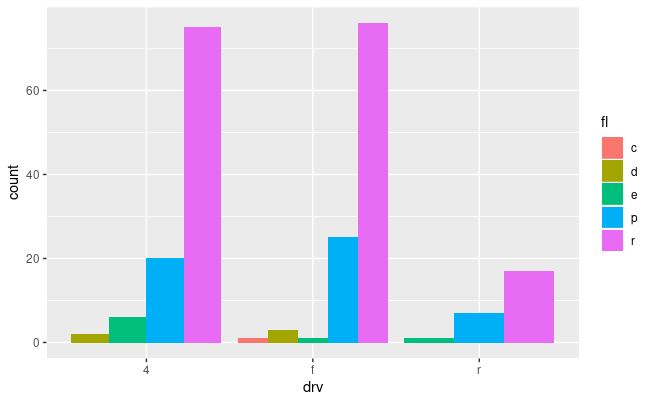
\includegraphics[width=\textwidth]{img/bivar-geclusterd-staafdiagram}
    \caption{Een geclusterd staafdiagram.}
    \label{fig:geclusterd-staafdiagram}
  \end{subfigure}
  \begin{subfigure}{.33\textwidth}
    \centering
    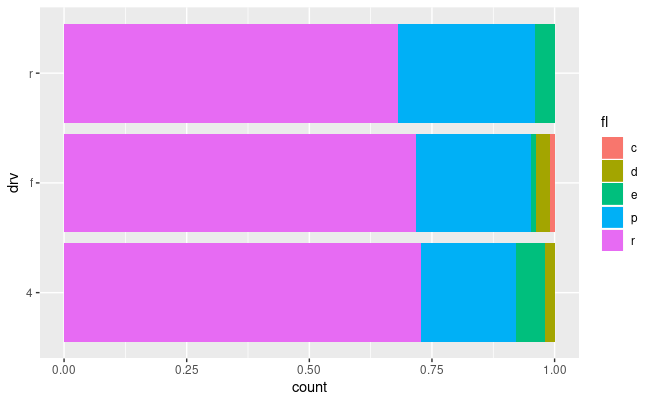
\includegraphics[width=\textwidth]{img/bivar-rependiagram}
    \caption{Een rependiagram.}
    \label{fig:rependiagram}
  \end{subfigure}
  \begin{subfigure}{.33\textwidth}
    \centering
    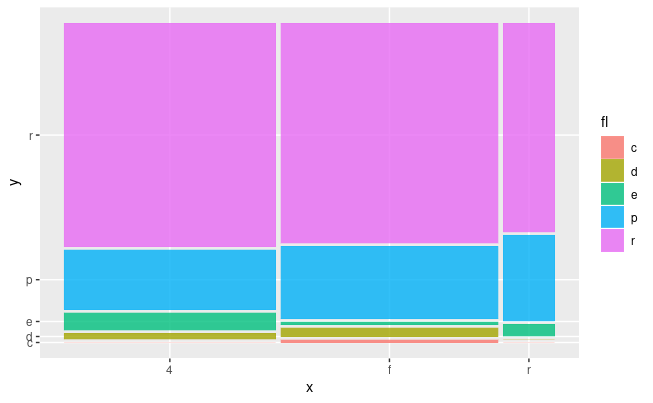
\includegraphics[width=\textwidth]{img/bivar-mozaiekdiagram}
    \caption{Een mozaïekdiagram.}
    \label{fig:mozaiekdiagram}
  \end{subfigure}
  \caption[Visualisatietechnieken voor 2 kwalitatieve variabelen]{Visualisatietechnieken voor 2 kwalitatieve variabelen. In deze grafieken wordt telkens dezelfde data getoond.}
\end{figure}


\section{Kwalitatief--kwantitatief}
\label{sec:kwal-kwant}

In deze sectie bekijken we methoden om na te gaan of er een verband bestaat tussen enerzijds een kwalitatieve variabele (onafhankelijk) en anderzijds een kwantitatieve variabele (afhankelijk). Een onderzoek naar genderongelijkheid bij verloning in de ict-sector is hier een goed voorbeeld van. De onafhankelijke variabele \emph{gender} is nominaal (mogelijke waarden bijvoorbeeld M/V/X), de afhankelijke variabele \emph{netto maandloon} is een ratio-variabele.

De benadering die men typisch gebruikt, is om het gemiddelde en/of standaardafwijking van de afhankelijke variabele tussen de verschillende groepen ontstaan uit de onafhankelijke met elkaar te vergelijken. Als de verschillen klein zijn, dan kunnen ze worden toegeschreven aan toevallige steekproeffouten en besluiten we dat er geen verband is. Als de verschillen groot zijn, dan besluiten we dat er \emph{wel} een verband is. Vaak is het bijvoorbeeld nog altijd zo dat mannen significant meer verdienen dan vrouwen voor een gelijkaardige job!

In deze cursus bespreken we de $t$-toets voor 2 steekproeven om te bepalen of er een verschil is tussen twee groepen (zie Sectie~\ref{ssec:t-toets-twee-steekproeven}). Er bestaan statistische toetsen om een groter aantal groepen tegelijk te beschouwen (bijvoorbeeld de ANOVA-toets), maar die vallen buiten het bestek van deze cursus.

Net zoals Cramér's V bij kwalitatieve variabelen bestaan er ook in dit geval metrieken die aangeven hoe sterk het verband is tussen kwalitatieve en kwantitatieve variabelen. In deze context worden die vaak onder de noemer \emph{effectgrootte} genoemd. In deze cursus zien we één definitie van effectgrootte, nl.~Cohen's $d$ (zie Sectie~\ref{ssec:cohens-d}). Opnieuw, er bestaan meerdere vormen van effectgrootte, ook geschikt voor variabelen met andere meetniveaus, maar deze vallen ook buiten het bestek van deze cursus.

\subsection{De \texorpdfstring{$t$}{t}-toets voor twee steekproeven}
\label{ssec:t-toets-twee-steekproeven}

De $t$-toets die geïntroduceerd werd in Sectie~\ref{sec:t-toets} kan ook gebruikt worden om twee steekproeven met elkaar te vergelijken. Je kan er dan mee nagaan of het steekproefgemiddelde van beide steekproeven \emph{significant} verschillend is.

Men maakt onderscheid tussen twee gevallen:

\begin{itemize}
  \item Beide steekproeven zijn onafhankelijk, zijn afzonderlijk genomen. Een voorbeeld is een onderzoek naar een medische behandelingsmethode waar een contolegroep de behandeling \emph{niet} krijgt en een testgroep de behandeling wel krijgt.
  \item De steekproeven zijn afhankelijk, of gepaard. Een voorbeeld is twee metingen uitvoeren op hetzelfde lid van de populatie, zoals de koorts nemen voor en na het innemen van een medicijn om het effect ervan te meten.
\end{itemize}

In R kan je eveneens de functie \texttt{t.test} gebruiken voor het uitvoeren van een toets met twee steekproeven. We geven hieronder twee voorbeelden, één voor elk geval.

\begin{example}
  In een klinisch onderzoek wil men nagaan of een nieuw medicijn als bijwerking een vertraagde (dus hogere) reactiesnelheid heeft~\autocite{Lindquist}.
  
  Zes deelnemers kregen een medicijn toegekend (interventiegroep) en zes anderen een placebo (controlegroep). Vervolgens werd hun reactietijd op een stimulus gemeten (in ms). We willen nagaan of er significante verschillen zijn tussen de interventie- en controlegroep.
  
  \textbf{Opmerking}: De interventiegroep en de controle groep zijn hier toevallig even groot (elk 6 proefpersonen).
  Dit is niet noodzakelijk. Bij een onafhankelijke (niet-gepaarde) steekproeven
  mogen de 2 groepen een verschillende grootte hebben.
  
  \begin{itemize}
    \item Controlegroep: 91, 87, 99, 77, 88, 91 ~~~~~~~~~~~~($\overline{x}=88,83$)
    \item Interventiegroep: 101, 110, 103, 93, 99, 104 ~~($\overline{y}=101,67$)
  \end{itemize}
  
  We noteren $\mu_1$ voor het gemiddelde van de niet behandelde populatie (controlegroep) en $\mu_2$ voor het populatiegemiddelde van de patiënten die het medicijn nemen (interventiegroep).
  
  De hypothesen worden formeel als volgt genoteerd:
  
  $H_0: \mu_1 - \mu_2 = 0$ en $H_1: \mu_1 - \mu_2 < 0$
  
  Als toetsingsgrootheid gebruiken we $\overline{x}-\overline{y}$, met $\overline{x}$ en $\overline{y}$ schattingen voor de \textit{\'echte} waarden $\mu_1$ en $\mu_2$ .
  
  Het gaat hier dus over een linkszijdige test, wat weergegeven wordt door de optie \texttt{alternative = "less"}. In de nulhypothese veronderstellen we dat het verschil tussen de populatiegemiddelden 0 is, wat met de optie \texttt{mu = 0} wordt aangeduid. Merk op dat dit de standaardwaarde is voor deze parameter en dus in principe niet moet worden opgegeven.
  
  \begin{lstlisting}
  controle <-  c(91, 87, 99, 77, 88, 91)
  interventie <- c(101, 110, 103, 93, 99, 104)
  t.test(controle, interventie, alternative="less", mu=0)
  \end{lstlisting}
  
  Het resultaat van de toets:
  
  \begin{verbatim}
  t.test(controle, interventie, alternative="less")
  
  Welch Two Sample t-test
  
  data:  controle and interventie
  t = -3.4456, df = 9.4797, p-value = 0.003391
  alternative hypothesis: true difference in means is less than 0
  95 percent confidence interval:
  -Inf -6.044949
  sample estimates:
  mean of x mean of y 
  88.83333 101.66667
  \end{verbatim}
  
  De teststatistiek $\overline{x}-\overline{y}=-12,833$ komt overeen met een $t$-waarde $t=-3,4456$.
  De parameter $df=9,48$ wordt bepaald door \texttt{t.test()} op basis van
  het aantal elementen in de reeksen $x$ en $y$.
  De berekening hiervan is \textit{niet} triviaal.
  
  De $p$-waarde, 0,003391, ligt duidelijk onder het significantieniveau (niet expliciet opgegeven, dus werd de standaardwaarde $\alpha = 0,05$ gebruikt.)
  
  We mogen dus de nulhypothese verwerpen en besluiten dat volgens de resultaten van deze steekproef het medicijn inderdaad een significant effect heeft op de reactiesnelheid van patiënten.
  
  \textbf{Opmerking}: Vermits $\overline{x}-\overline{y}=-12,833$
  kunnen we met 95\% procent zekerheid zeggen dat het verschil van de \textit{\'echte} gemiddelden ($\mu_1-\mu_2$)
  van een grotere controle- en interventiepopulatie tussen $-\infty$ en $-6.044949$ zal liggen.
  Zie paragraaf \ref{ssec:betrouwbaarheidsinterval-grote-steekproef} (p. \pageref{ssec:betrouwbaarheidsinterval-grote-steekproef})
  en \ref{ssec:betrouwbaarheidsinterval-kleine-steekproef} (p. \pageref{ssec:betrouwbaarheidsinterval-kleine-steekproef})
  over betrouwbaarheidsintervallen.
\end{example}

\begin{example}
  In een studie werd nagegaan of auto's die rijden op benzine met additieven ook een lager verbruik hebben. Tien auto's werden eerst volgetankt met ofwel gewone benzine, ofwel benzine met additieven (bepaald door opgooien van een munt), waarna het verbruik werd gemeten (uitgedrukt in mijl per gallon). Vervolgens werden de auto's opnieuw volgetankt met de andere soort benzine en werd opnieuw het verbruik gemeten. De resultaten worden gegeven in de tabel hieronder.
  
  \begin{center}
    \begin{tabular}{|l|c|c|c|c|c|c|c|c|c|c|}
      \hline 
      Auto & 1 & 2 & 3 & 4 & 5 & 6 & 7 & 8 & 9 & 10 \\ 
      \hline 
      Gewone benzine & 16 & 20 & 21 & 22 & 23 & 22 & 27 & 25 & 27 & 28 \\ 
      \hline 
      Additieven & 19 & 22 & 24 & 24 & 25 & 25 & 25 & 26 & 28 & 32 \\ 
      \hline 
    \end{tabular} 
    %  \caption{Verbruik in mijl per gallon met 2 soorten benzine.}
    %  \label{tab:benzineverbruik-additieven}
  \end{center}
  
  We gaan door middel van een \emph{gepaarde $t$-test} na of auto's significant zuiniger rijden met benzine met additieven.
  
  We kiezen $x$ voor benzine met \texttt{additieven} ($\overline{x}=25,1$ mijl per gallon), en we kiezen $y$ voor \texttt{gewone} bezine ($\overline{y}=23,1$ mijl per gallon).
  
  De nulhypothese $H_0$ is dat je met beiden even veel mijl per gallon kunt rijden ($\mu_{x-y}=0$).
  De alternatieve hypothese $H_1$ dat je verder kunt rijden op benzine met additieven ($\mu_{x-y}>0$).
  
  De optie \texttt{paired=TRUE} geeft aan dat het hier om een gepaarde $t$-toets gaat.
  
  \begin{lstlisting}
  gewone    <- c(16, 20, 21, 22, 23, 22, 27, 25, 27, 28)
  additieven <-c(19, 22, 24, 24, 25, 25, 26, 26, 28, 32)
  t.test(additieven, gewone, alternative="greater", paired=TRUE)
  \end{lstlisting}
  
  Resultaat:
  
  \begin{verbatim}
  Paired t-test
  
  data:  additieven and gewone
  t = 4.4721, df = 9, p-value = 0.0007749
  alternative hypothesis: true difference in means is greater than 0
  95 percent confidence interval:
  1.180207      Inf
  sample estimates:
  mean of the differences 
  2 
  \end{verbatim}
  
  De teststatistiek $\overline{x-y}=2$. Dit komt overeen met een $t$-waarde $t=4,4721$.
  De $p$-waarde, 0,0007749, ligt onder het significantieniveau ($\alpha=0,05$), dus we kunnen de nulhypothese verwerpen. Volgens deze steekproef rijden auto's inderdaad zuiniger met benzine met additieven.
  
  \textbf{Ter info}: Bij 95\% van de ``paren'' van een grotere populatie auto's,
  zal het verschil $x-y$ tussen $1.180207$ en $+\infty$ liggen.
  Dit is het betrouwbaarheidsinterval waarvan sprake in paragraaf \ref{ssec:betrouwbaarheidsinterval-grote-steekproef} (p. \pageref{ssec:betrouwbaarheidsinterval-grote-steekproef})
  en \ref{ssec:betrouwbaarheidsinterval-kleine-steekproef} (p. \pageref{ssec:betrouwbaarheidsinterval-kleine-steekproef}).
\end{example}

\subsection{Effectgrootte - Cohen's \texorpdfstring{$d$}{d}}
\label{ssec:cohens-d}

Met de term \emph{effectgrootte}\index{effectgrootte} bedoelt men een metriek die de impact (of effect) van een gebeurtenis weergeeft. Bij de meeste varianten geeft een grote absolute waarde ook een groter effect aan, een waarde van 0 het ontbreken van een effect.

In deze sectie introduceren we Cohen's $d$\index{Cohen's $d$}, ontwikkeld door de Amerikaanse psycholoog en statisticus Jacob Cohen\index{Cohen, Jacob}. Deze metriek wordt in het bijzonder vaak gebruikt in publicaties over onderzoek naar effecten op leerresultaten in het onderwijs. Een onderzoek in deze context wordt vaak als volgt opgezet:

De onderzoekers wensen het effect te weten van een bepaalde interventie op het leren van studenten/leerlingen. Ze willen bijvoorbeeld een nieuwe lesvorm uitproberen en bepalen of die geschikt is. Er worden testpersonen geselecteerd die typisch aselect verdeeld worden over twee groepen: een controlegroep die een afgebakend stuk leerstof te verwerken krijgt op een ``klassieke'' manier en een interventiegroep die dezelfde leerstof volgens die nieuwe lesvorm krijgt voorgeschoteld. Na afloop van de lessen volgt er dan een toets om te bepalen in hoeverre de studenten van beide groepen de leerstof verworven hebben. We verwachten dan dat de studenten uit de interventiegroep een significant beter resultaat behalen dan de controlegroep. In de wetenschappelijke publicaties die resulteren uit dit soort onderzoek wordt steevast de effectgrootte gepubliceerd.

John \textcite{Hattie2012}\index{Hattie, John} verzamelt al decennia lang publicaties over onderzoek in onderwijs en houdt een lijst bij van effectgroottes van allerlei dingen die impact hebben op studieresultaten bij studenten. Dat gaat niet alleen over lesmethodes, maar ook leerstrategieën van studenten, demografische factoren (gender, sociale status, enz.), school- en klasmanagement, enz. In zijn meta-analyse hebben de meeste bestudeerde factoren een positief effect op de leerresultaten, wat misschien wel een gevolg kan zijn van \emph{publication bias}. 

De gemiddelde gerapporteerde effectgrootte ligt rond $d = 0,4$. De aanbeveling van Hattie is dan ook dat scholen die een positief effect op leerresultaten van studenten willen bekomen, best eerst kijken naar de factoren die resulteren in een effectgrootte van minstens 0,4. Als vuistregel kan je stellen dat een interventie met $d = 1$ als gevolg heeft dat de leerstof die normaal op één jaar gezien wordt, op de helft van de tijd kan verwerkt worden. Tabel~\ref{table:effectgrootte} geeft een overzicht van de interpretatie van verschillende waarden voor Cohen's $d$.

\begin{definition}[Cohen's $d$]
  is gedefinieerd als het verschil tussen twee gemiddelden gedeeld door een standaardafwijking voor de steekproef, meer bepaald:
  \begin{equation}
  d = \frac{\overline{x}_1 - \overline{x}_2}{s}
  \end{equation}
  
  met $\overline{x}_1$ en $\overline{x}_2$ de gemiddelden van beide groepen en $s$ een gecombineerde standaardafwijking voor twee onafhankelijke steekproeven:
  
  \begin{equation}
  s = \sqrt{\frac{(n_1 - 1) s_1^2 + (n_2 - 1) s_2^2}{n_1 + n_2 - 2}}
  \end{equation}
  
  met $s_1^2$ en $s_2^2$ de steekproefvariantie van beide groepen en $n_1$ en $n_2$ het aantal observaties in elke groep.
\end{definition}

\begin{table}
  \centering
  \begin{tabular}{rl}
    \toprule
    \textbf{$|d|$} & \textbf{Effect} \\
    \midrule
    0,01 & Zeer klein \\
    0,20 & Klein \\
    0,50 & Middelmatig \\
    0,80 & Groot \\
    1,20 & Zeer groot \\
    2,00 & Reusachtig \\
    \bottomrule
  \end{tabular}
  \caption{Interpretatie van de absolute waarde van Cohen's $d$. Merk op dat $d$ ook kleiner dan 0 kan zijn, wat wijst op een negatief effect van de interventie.}
  \label{table:effectgrootte}
\end{table}

\subsection{Visualisatietechnieken}
\label{ssec:kwal-kwant-visualisatie}

\subsubsection{Boxplot}

% TODO   Boxplot

\subsubsection{Staafdiagram met error bars}

% TODO  Staafdiagram met error bars

\section{Kwantitatief--kwantitatief}

% TODO: inleiding
% TODO: Spreidingsdiagram

\subsection{Regressie}
\label{sec:regressie}

Bij \index{Regressie} regressie gaan we proberen een consistente en systematische koppeling tussen de variabelen te vinden. Dat betekent concreet: ``als we de waarde van de onafhankelijke variabele kennen, kunnen we dan ook de waarde van de afhankelijke variabele voorspellen?'' We kennen twee soorten verbanden:

\begin{description}
  \item [Monotoon:] een monotoon verband is een verband waarbij de onderzoeker de algemene richting van de samenhang tussen de twee variabelen kan aanduiden, hetzij stijgend, hetzij dalend. De richting van het verband verandert nooit.
  \item [Niet-monotoon:] bij een niet-monotoon verband wordt de aanwezigheid (of afwezigheid) van de ene variabele systematisch gerelateerd aan de aanwezigheid (of afwezigheid) van een andere variabele. De richting van het verband kan echter niet aangeduid worden.
\end{description}

Bij lineaire regressie gaan we ons beperken tot een lineair verband: een rechtlijnige samenhang tussen een onafhankelijke en afhankelijke variabele, waarbij kennis van de onafhankelijke variabele kennis over de afhankelijke variabele geeft.

Bij een lineair verband zijn er drie karakteristieken:

\begin{enumerate}
  \item Aanwezigheid: is er wel een verband tussen de twee variabelen?
  \item Richting: is er een dalend of een stijgend verband?
  \item Wat is de sterkte van het verband: sterk, gematigd of niet-bestaand?
\end{enumerate}

Een voorbeeld van een linear verband $y = \beta_{0} + \beta_{1}x$  vind je bijvoorbeeld in figuur \ref{fig:regressieFig}.

\begin{figure}[t]
  \begin{tikzpicture}
    \begin{axis}[
        axis x line=middle,
        axis y line=middle,
        enlarge y limits=true,
        width=\textwidth, height=8cm,     % size of the image
        grid = major,
        grid style={dashed, gray!30},
        ylabel=$y$,
        xlabel=$x$,
        legend style={at={(0.1,-0.1)}, anchor=north}
      ]
      \addplot[only marks] table  {data/regressie.dat};
      \addplot [no markers, thick, red] table [y={create col/linear regression={y=y}}] {data/regressie.dat};
    \end{axis}
  \end{tikzpicture}
  \caption{Een voorbeeld van een lineair verband}
  \label{fig:regressieFig}
\end{figure}

Zo'n verband kunnen we vinden aan de hand van de \index{Kleinste kwadraten methode} kleinste kwadraten methode van Gauss. Dit wordt als volgt gedaan.

\begin{theorem}

  Een lineair verband wordt weergegeven als volgt:

  \begin{equation}
    y = \beta_{0} + \beta_{1} x
    \label{eq:lineair}
  \end{equation}
  met
  \begin{itemize}
    \item $y$ de afhankelijke
    \item $x$ de onafhankelijke
  \end{itemize}

  We willen hier de som van de kwadraten minimaliseren van de afwijkingen $e_{i} = y_{i} - (\beta_{0} + \beta_{1}x_{i})$. Zo'n afwijking kan ook geschreven worden als (stel $X_{i} = x_{i} - \overline{x}$ en $Y_{i} = y_{i} - \overline{y}$):

  \begin{eqnarray}
    e_{i} & = & y_{i} - \beta_{1} x_{i} - \beta_{0} \\
    e_{i} & = & (y_{i} - \overline{y}) - \beta_{1}(x_{i} - \overline{x}) - (\beta_{0} - \overline{y} + \beta_{1} \overline{x}) \\
    \label{eq:regressie-bewijs}
    e_{i} & = & Y_{i} - \beta_{1} X_{i} - (\beta_{0} - \overline{y} + \beta_{1} \overline{x})
  \end{eqnarray}

  In stap~\ref{eq:regressie-bewijs} doen we eigenlijk $+\overline{x}-\overline{x}+\overline{y}-\overline{y}$, wat een nuloperatie is. Dit is een gedachtensprong die niet meteen voor de hand ligt, maar onthou dat dit een ``shortcut'' is naar de oplossing en dat het ``echte'' bewijs een stuk ingewikkelder is.

  We willen de som van de kwadraten van $e_i$  minimaliseren:

  \begin{eqnarray}
    \sum_{i}^{n} e_{i}^{2} & =& \sum_{i}^{n} (y_{i} - (\beta_{0} + \beta_{1}x_{i}))^{2}\\
    & = & \sum_{i}^{n} ((Y_{i} - \beta_{1} X_{i}) - (\beta_{0} - \overline{y} + \beta_{1}\overline{x}))^{2}\\
    & = & \sum_{i}^{n}(Y_{i} - \beta_{1} X_{i})^2 - 2 \sum_{i}^{n}(Y_i - \beta_1 X_i)(\beta_0 - \overline{y}+ \beta_1\overline{x}) + \sum_{i}^{n}(\beta_{0} - \overline{y} + \beta_{1}\overline{x})^{2} \label{eq:stap1}\\
    & = & \sum_{i}^{n}(Y_{i} - \beta_{1} X_{i})^{2} + n(\beta_{0} - \overline{y} + \beta_{1} \overline{x})^{2} \label{eq:stap2}
  \end{eqnarray}
	
	We kunnen de stap maken van \ref{eq:stap1} naar \ref{eq:stap2} door volgende uit te werken:
	
\[ \sum_{i}^{n}X_i = \sum_{i}^{n} (x_i - \overline{x}) = 0 \]
	en equivalent
\[ \sum_{i}^{n}Y_i = \sum_{i}^{n} (y_i - \overline{y}) = 0 \]
daardoor is
\[ \sum_{i}^{n}(Y_i - \beta_1 X_i) = \sum_{i}^{n}Y_i - \beta_1 \sum_{i}^{n}X_i = 0 \]
en bijgevolg dus ook
\[ 2 \sum_{i}^{n}(Y_i - \beta_1 X_i)(\beta_0 - \overline{y}) \]
	

Nu is $e^{2}_{i}$ geschreven als een som van twee positieve uitdrukkingen. Deze som is minimaal als beide uitdrukkingen minimaal zijn.

  \begin{equation}
    \begin{cases}
      \sum_{i}^{n}( Y_{i} - \beta_{1} X_{i})^{2} \textnormal{ is minimaal.}\\
      n(\beta_{0} - \overline{y} + \beta_{1} \overline{x})^{2} \textnormal{ is minimaal}
    \end{cases}
    \label{eq:vgl}
  \end{equation}
	

Voor de eerste uitdrukking vinden we eigenlijk een kwadratische functie in $\beta_1$.
  \begin{eqnarray}
		& \sum_{i}^{n}( Y_{i} - \beta_{1} X_{i})^{2} \textnormal{ is minimaal.} \label{eq:uitdrukking}\\
		\Leftrightarrow & \sum_i^n (Y_i^2 - 2X_iY_i\beta_1 + X_i^2\beta_1^2) \textnormal{ is minimaal.} \\
		\Leftrightarrow & \beta_1^2 \sum_i^n X_i^2 - 2\beta_1 \sum_i^n X_iY_i + \sum_i^nY_i^2 \textnormal{ is minimaal.} \\
		\Leftrightarrow & \textnormal{is minimaal als } \beta_{1} = \frac{\sum_{i}^{n} X_{i}Y_{i}}{\sum_{i}^{n} X_{i}^{2}}
	\end{eqnarray}

Voor de tweede uitdrukking vinden we

  \begin{eqnarray}
		& n(\beta_{0} - \overline{y} + \beta_{1} \overline{x})^{2} \textnormal{ is minimaal}
		\Leftrightarrow & n(\beta_{0} - \overline{y} + \beta_{1} \overline{x})^{2} = 0 \\
		\Leftrightarrow & \beta_{0} - \overline{y} + \beta_{1} \overline{x} = 0 \\
		\Leftrightarrow & \beta_{0} = \overline{y} - \beta_{1}\overline{x} 
	\end{eqnarray}

	
  met als oplossing

  \begin{equation}
    \begin{cases}
      \beta_{1} = \frac{\sum_{i}^{n} X_{i}Y_{i}}{\sum_{i}^{n} X_{i}^{2}}\\
      \beta_{0} = \overline{y} - \beta_{1}\overline{x}
    \end{cases}
    \label{eq:vgl2}
  \end{equation}

  en dus

  \begin{eqnarray}
    \beta_{1} & = & \frac{\sum_{i}^{n} (x_{i} - \overline{x})(y_{i} - \overline{y})}{\sum_{i}^{n} (x_{i} - \overline{x})^{2}} \\
    \beta_{0} & = & \overline{y} - \beta_{1} \overline{x}
    \label{eq:regressie}
  \end{eqnarray}
\end{theorem}


\begin{table} \centering
  \begin{tabular}{@{}rr@{}} \toprule
    Eiwitgehalte\%& Gewichtstoename (gram)  \\
    \midrule
    0		&	177 \\
    10 	&	231	\\
    20	& 249	\\
    30	& 348 \\
    40	& 361 \\
    50	& 384 \\
    60	& 404 \\
    \bottomrule
  \end{tabular}
  \caption{De data die verzameld geweest is door de kerstman: per eiwitpercentage wordt de gewichtstoename beschouwd.}
  \label{tab:rendieren}
\end{table}



\begin{table} \centering
  \begin{tabular}{@{}llllll@{}}
    \toprule
    $x$   & $y$     & $x-\overline{x}$    & $y - \overline{y}$        & $(x-\overline{x})(y - \overline{y})$       &  $(x-\overline{x})^{2}$    \\ \midrule
    0  & 177 & -30 & -130,71 & 3921,3 & 900  \\
    10 & 231 & -20 & -76,71  & 1534,2 & 400  \\
    20 & 249 & -10 & -58,71  & 587,1  & 100  \\
    30 & 348 & 0   & 40,29   & 0      & 0    \\
    40 & 361 & 10  & 53,29   & 532,9  & 100  \\
    50 & 384 & 20  & 76,29   & 1525,8 & 400  \\
    60 & 404 & 30  & 96,29   & 2888,7 & 900  \\
    &     &     &         & 10990  & 2800 \\ \bottomrule
  \end{tabular}
  \caption{Berekeningen die nodig zijn voor het toepassen van de kleinste kwadratenmethode.}
  \label{tab:rendieren2}
\end{table}

\begin{figure}
  \begin{tikzpicture}
    \begin{axis}[
        axis x line=middle,
        axis y line=middle,
        enlarge y limits=true,
        width=\textwidth, height=8cm,     % size of the image
        grid = major,
        grid style={dashed, gray!30},
        ylabel=gewichtstoename (g),
        xlabel=eiwitgehalte (\%),
        legend style={at={(0.1,-0.1)}, anchor=north}
      ]
      \addplot[only marks] table  {data/santa.txt};
      \addplot [no markers, thick, red] table [y={create col/linear regression={y=y}}] {data/santa.txt};
    \end{axis}
  \end{tikzpicture}

  \caption{Lineair verband tussen eiwitgehalte en gewichtstoename}
  \label{fig:rendierenFiguur}
\end{figure}

\begin{example}
  \label{vb:rendieren}
  We kijken naar het voorbeeld van de Kerstman en zijn rendieren. Hij wil zien of er een lineair verband bestaat tussen het eiwitgehalte van het voeder en de gewichtstoename van de rendieren. Hij voert een aantal proeven uit en bekomt de data in tabel \ref{tab:rendieren}. Door toepassing van de formules die hierboven staan bekomt men (zie tabel \ref{tab:rendieren2}):
  \[ \beta_{1} = \frac{\sum_{i=1}^{n} (x_{i}-\overline{x})(y_{i} - \overline{y})}{\sum_{i=1}^{n} (x_{i}-\overline{x})^{2}} = \frac{10990}{2800} = 3.925 \]
  \[ \beta_{0} = \overline{y} - \beta_{1} \overline{x} = 307.7143 - 3.925 \times 30 = 189.96 \]
  Men heeft dus een lineair verband gevonden die de kwadraten van de residuen minimaliseert. Let wel, er wordt niets gezegd over de sterkte of validiteit van dit verband. Dit verband wordt getekend in figuur \ref{fig:rendierenFiguur}.
\end{example}

Voorbeeld~\ref{vb:rendieren} uitgewerkt in R (met plot van de regressierechte):

\lstinputlisting{data/regressie.R}

\subsection{Correlatie}
\label{sec:correlatie}

\subsubsection{Pearsons product-momentcorrelatiecoëfficiënt}

We kunnen twee statistieken bepalen die de sterkte van een lineair verband uitdrukken. Ook deze zijn---net als de $\chi^2$-toets---ontwikkeld door Karl Pearson\index{Pearson!Karl}.

\begin{definition}[Pearsons product-momentcorrelatiecoëfficiënt]
   Pearsons product momentcorrelatiecoëfficiënt\index{Pearsons product-momentcorrelatiecoëfficiënt} $R$ (of kortweg correlatiecoëfficiënt\index{correlatiecoëfficiënt}) is een maat voor de sterkte van de lineaire samenhang tussen X en Y. De waarde kan vari\"eren van -1 tot 1.

  \begin{itemize}
    \item Een waarde van +1 duidt een positief lineair verband aan.
    \item Een waarde van -1 duidt een negatief lineair verband aan.
    \item Een waarde van 0 wil zeggen dat er totaal geen lineaire samenhang is.
  \end{itemize}
  
  Hoe dichter de correlatiecoëfficiënt bij 1 of -1, hoe beter de kwaliteit van het lineair model.
\end{definition}

\subsubsection{Determinatieco\"effici\"ent}

\begin{definition}
  De \index{Determinatieco\"effici\"ent}determinatieco\"effici\"ent ($R^{2}$) is het kwadraat van de correlatieco\"effici\"ent en verklaart het percentage van de variantie van de waargenomen waarden t.o.v. de regressierechte.

  \begin{itemize}
    \item $R^{2}$ is de verklaarde variantie
    \item $1-R^{2}$ is de onverklaarde variantie
  \end{itemize}
\end{definition}

\begin{figure}[t]
  \begin{tikzpicture}
    \begin{axis}[
        axis x line=middle,
        axis y line=middle,
        enlarge y limits=true,
        width=\textwidth, height=8cm,     % size of the image
        grid = major,
        grid style={dashed, gray!30},
        ylabel=gezinsgrootte moeder,
        xlabel=gezinsgrootte,
        legend style={at={(0.1,-0.1)}, anchor=north}
      ]
      \addplot[only marks] table  {data/families.txt};
      \addplot [no markers, thick, red] table [y={create col/linear regression={y=y}}] {data/families.txt};
    \end{axis}
  \end{tikzpicture}
  \caption{Linear verband tussen grootte van een gezin en de grootte van de familie van de moeder}
  \label{fig:moederVerband}
\end{figure}

\tikzset{small dot/.style={fill=black, circle,scale=0.2}}
\tikzset{every pin/.style={draw=black,fill=yellow!10}}

\begin{figure}[t]%
  \begin{tikzpicture}
    \begin{axis}[
        axis x line=middle,
        axis y line=middle,
        enlarge y limits=true,
        width=\textwidth, height=8cm,     % size of the image
        grid = major,
        grid style={dashed, gray!30},
        ylabel=gezinsgrootte moeder,
        xlabel=gezinsgrootte,
        legend style={at={(0.1,-0.1)}, anchor=north}
      ]
      \draw (axis cs:3,0)--(axis cs:3,8);
      \draw (axis cs:0,4.3)--(axis cs:6,4.3);
      \node[small dot, pin=120:{$III$}] at (axis cs:1.6,7) {};
      \node[small dot, pin=120:{$I$}] at (axis cs:5.5,7) {};
      \node[small dot, pin=120:{$II$}] at (axis cs:1.6,2) {};
      \node[small dot, pin=120:{$IV$}] at (axis cs:5.5,2) {};
      \addplot[only marks] table  {data/families.txt};
    \end{axis}
  \end{tikzpicture}
  \caption{De figuur opgedeeld in 4 kwadranten}%
  \label{fig:kwadranten}%
\end{figure}

\subsubsection{Bepaling van $R$ en $R^{2}$}
\label{sec:determinatiecoef}
Beschouw het voorbeeld in figuur \ref{fig:moederVerband}:  de grootte van een gezin vs. de grootte van het gezin van de moeder. We zien duidelijk dat er een linear verband is. Indien we de gemiddelde berekenen en de figuur in 4 kwadranten (kwadrant $I$, $II$, $III$, $IV$) volgens de gemiddelden verdelen krijgen we de figuur in \ref{fig:kwadranten}.  Dan kunnen we volgende situaties bekijken.

\begin{itemize}
  \item Neem een element uit gebied I. Voor dit element is $x_{i} - \overline{x}$ positief en $y_{i} - \overline{y}$ ook. Dus is hun product. $(x_{i} - \overline{x}) (y_{i} - \overline{y}) > 0$.
  \item Neem een element uit gebied II. Voor dit element is $x_{i} - \overline{x}$ negatief en $y_{i} - \overline{y}$ ook. Dus is hun product. $(x_{i} - \overline{x}) (y_{i} - \overline{y}) > 0$.
  \item Neem een element uit gebied III. Voor dit element is $x_{i} - \overline{x}$ negatief en $y_{i} - \overline{y}$ positief. Dus is hun product. $(x_{i} - \overline{x}) (y_{i} - \overline{y}) < 0$.
  \item Neem een element uit gebied IV. Voor dit element is $x_{i} - \overline{x}$ positief en $y_{i} - \overline{y}$ negatief. Dus is hun product. $(x_{i} - \overline{x}) (y_{i} - \overline{y}) < 0$.
\end{itemize}

Aangezien dat er meer punten in gebieden I en II zijn dan in gebieden III en IV zal de som $\sum_{i} (x_{i} - \overline{x}) (y_{i} - \overline{y})$ een positief getal zijn. Hoe meer punten in I en II, hoe groter het getal. We merken dus een sterk positief lineair verband.

Indien de punten ongeveer gelijk verdeeld zouden zijn over de vier gebieden vinden we dat deze soms dicht bij nul zal zijn. Omgekeerd, indien er een negatief lineair verband zou zijn vinden we een negatief getal.

We hebben dus een maat gevonden om het verband tussen twee variabelen te meten:

\begin{itemize}
  \item Stijgende gecorreleerde verbanden is $\sum_{i} (x_{i} - \overline{x}) (y_{i} - \overline{y})$ positief en groot.
  \item Dalende gecorreleerde verbanden is $\sum_{i} (x_{i} - \overline{x}) (y_{i} - \overline{y})$ negatief en groot (in absolute waarde).
  \item Met niet gecorreleerde variabelen is $\sum_{i} (x_{i} - \overline{x}) (y_{i} - \overline{y})$ klein in absolute waarde.
\end{itemize}

We kunnen deze maat onafhankelijk maken van de grootte van de steekproef door te delen door de steekproefgrootte $n$. Dit noemen we de co-variantie en wordt gedefinieerd als gemeenschappelijke spreiding:

\begin{equation}
  Cov(X,Y) = \frac{\sum_{i}^{n}(x_{i} - \overline{x}) (y_{i} - \overline{y})}{n}
  \label{eq:covariantie}
\end{equation}

Dit geeft ons de gemiddelde afwijking per meetpunt.

Om opnieuw te normaliseren (een variatie in X is niet per se van dezelfde grootteorde als een variatie in Y) gaan we de maatstaf voor het gezamelijk vari\"eren onafhankelijk maken van het aantal waarnemingen en de orde van grootte van de getalswaarden. Zo kunnen we deze waarden universeel vergelijkbaar maken. Daarom delen we de co-variantie door het product van de standaardafwijkingen en noemen we de relatieve co-variantie of Pearson's correlatieco\"effici\"ent ook bekend als product-moment-correlatieco\"effici\"ent of kortweg als correlatieco\"effici\"ent.

\begin{eqnarray}
  R &=&\frac{COV(X,Y)}{\sigma_{x}\sigma_{y}} \\
  &=& \frac{COV(X,Y)}{\sqrt{\frac{\sum(x_{i} - \overline{x})^{2}}{n}} \times \sqrt{\frac{\sum(y_{i} - \overline{y})^{2}}{n}}} \\
  &=& \frac{\sum_{i}^{n}(x_{i}-\overline{x})(y_{i} - \overline{y})}{\sqrt{\sum_{i}^{n} (x_{i}-\overline{x})^{2}} \sqrt{\sum_{i}^{n} (y_{i}-\overline{y})^{2}}}
  \label{eq:relCovar}
\end{eqnarray}

De correlatieco\"effici\"ent is onafhankelijk van de meeteenheid terwijl de covariantie afhankelijk is van de meeteenheid.

\subsubsection{Interpretatie van $R^{2}$}

Als we aannemen dat $x$ niet bijdraagt aan de voorspelling van $y$, dan is de beste voorspelling voor een waarde van $y$ het steekproefgemiddelde $\overline{y}$, dat in figuur \ref{fig:rendierenFiguur3} als een horizontale lijn wordt weergegeven. De verticale lijnstukken zijn de afwijkingen van de waargenomen punten $y$ van deze voorspelling (het steekproefgemiddelde). De som van de kwadraten van deze afwijkingen is:

\[ SS_{yy} = \sum(y_{i} - \overline{y})^{2} \]

Indien we aannemen dat $x$ wel een rol speelt bij de voorspelling van $y$, berekenen we de regressielijn bij dezelfde gegevensverzameling en de afwijkingen van de punten ten opzichte van de lijn zoals in figuur \ref{fig:rendierenFiguur2}.

\[ SSE_{yy} = \sum(y_{i} - \widehat{y})^{2} \]

 Als we nu de afwijkingen vergelijken met elkaar zien we het volgende:
\begin{enumerate}
  \item Als $x$ weinig of niet bijdraagt in de voorspelling zullen de sommen van de kwadraten van de afwijkingen van de twee lijnen nagenoeg dezelfde zijn:
    \[ SS_{yy} = \sum(y_{i} - \overline{y})^{2} \] en
    \[ SSE_{yy} = \sum(y_{i} - \widehat{y})^{2} \]
    waarbij $\widehat{y}$ de voorspelde waarde is.
  \item Als $x$ wel bijdraagt tot de voorspelling van $y$ zal $SSE_{yy}$ kleiner zijn dan $SS_{yy}$. In feite zal
    \[	SSE_{yy} = \sum(y_{i} - \widehat{y})^{2} \]
    gelijk zijn aan nul als alle punten perfect voorspeld worden (en dus op de regressierechte liggen).
\end{enumerate}

De vermindering in de som van de kwadraten die toegeschreven kan worden aan het opnemen van $x$ in het model is dan (uitgedrukt in fractie van $SS_{yy}$)
\[ \frac{SS_{yy} - SSE_{yy}}{SS_{yy}} \]
We noemen $SS_{yy}$ de totale steekproefvariantie van de meetwaarden rond het steekproefgemiddelde $\overline{y}$ en $SSE_{yy}$ de overblijvende niet-verklaarde steekproefvariantie, na het schatten van de lijn $\widehat{y} = \beta_{0} + \beta_{1}x$. Dus dan is $(SS_{yy} - SSE_{yy})$ de verklaarde variantie die toe te schrijven is aan de lineaire relatie met $x$.

Er kan nu worden aangetoond dat bij enkelvoudige lineaire regressie deze fractie
\[ \frac{SS_{yy} - SSE_{yy}}{SS_{yy}} = \frac{\textnormal{verklaarde variantie}}{\textnormal{totale steekproefvariantie}} \]
gelijk is aan het kwadraat van de Pearson correlatieco\"effici\"ent.  (= het deel van de totale variantie dat verklaard wordt door de lineaire rechte).

Tabel~\ref{tab:interpretatie-correlatiecoefficient} geeft een overzicht hoe de waarden van $R$ en $R^2$ kunnen geïnterpreteerd worden, meer bepaald hoe sterk het verband tussen twee variabelen dan is.

\begin{figure}
  \begin{tikzpicture}
    \begin{axis}[
        axis x line=middle,
        axis y line=middle,
        enlarge y limits=true,
        width=\textwidth, height=8cm,     % size of the image
        grid = major,
        grid style={dashed, gray!30},
        ylabel=eiwitgehalte,
        xlabel=gewichtstoename(gram),
        legend style={at={(0.1,-0.1)}, anchor=north}
      ]
      \addplot[only marks] table  {data/santa.txt};
      \addplot [no markers, thick, red] table [y={create col/linear regression={y=y}}] {data/santa.txt};
      \addplot [mark=none, color=red] coordinates {
        (0,177) (0,189.9643)
      };
      \addplot [mark=none, color=red] coordinates {
        (10,231) (10,229.2143)
      };
      \addplot [mark=none, color=red] coordinates {
        (20,249) (20,268.4643)
      };
      \addplot [mark=none, color=red] coordinates {
        (30,348) (30,307.7143)
      };
      \addplot [mark=none, color=red] coordinates {
        (40,361) (40,346.9643)
      };
      \addplot [mark=none, color=red] coordinates {
        (50,384) (50,386.2143)
      };
      \addplot [mark=none, color=red] coordinates {
        (60,404) (60,425.4643)
      };

    \end{axis}
  \end{tikzpicture}
  \caption{Deviaties tot de regressierechte: aanname $x$ geeft extra informatie voor het voorspellen van $y$.}
	\label{fig:rendierenFiguur2}
\end{figure}

\begin{figure}
  \begin{tikzpicture}
    \begin{axis}[
        axis x line=middle,
        axis y line=middle,
        enlarge y limits=true,
        width=\textwidth, height=8cm,     % size of the image
        grid = major,
        grid style={dashed, gray!30},
        ylabel=eiwitgehalte,
        xlabel=gewichtstoename(gram),
      ]
      \addplot[only marks] table  {data/santa.txt};
      \addplot [mark=none, color=black] coordinates {
        (0,307.71) (60,307.71)
      };
      \addplot [mark=none, color=red] coordinates {
        (0,177) (0,307.71)
      };
      \addplot [mark=none, color=red] coordinates {
        (10,231) (10,307.71)
      };
      \addplot [mark=none, color=red] coordinates {
        (20,249) (20,307.71)
      };
      \addplot [mark=none, color=red] coordinates {
        (30,348) (30,307.71)
      };
      \addplot [mark=none, color=red] coordinates {
        (40,361) (40,307.71)
      };
      \addplot [mark=none, color=red] coordinates {
        (50,384) (50,307.71)
      };
      \addplot [mark=none, color=red] coordinates {
        (60,404) (60,307.71)
      };

    \end{axis}
  \end{tikzpicture}
  \caption{Deviaties tot de gemiddelde van y: aanname $x$ geeft geen informatie voor het voorspellen van $y$ ($\overline{y} =307.71$).}
	  \label{fig:rendierenFiguur3}
\end{figure}

\begin{table} \centering \small
  \begin{tabular}{@{}rrrl} \toprule
    $|R|$ & $R^{2}$ & Verklaarde variantie &  Interpretatie \\
    \midrule
    $< 0,3$       & $< 0,1$       & $< 10\%$    & zeer zwak \\
    $0,3 - 0,5$   & $0,1 - 0,25$ & $10 - 25\%$ & zwak \\
    $0,5 - 0,7$   & $0,25 - 0,5$  & $25 - 50\%$ & matig\\
    $0,7 - 0,85$  & $0,5 - 0,75$  & $50 - 75\%$ & sterk\\
    $0,85 - 0,95$ & $0,75 - 0,9$  & $75 - 90\%$ & zeer sterk\\
    $> 0,95$      & $> 0,9$       & $>90\%$     & uitzonderlijk(!)\\
    \bottomrule
  \end{tabular}
  \caption[Interpretatie van $R$ en $R^2$.]{Interpretatie van $R$ en $R^2$.}
  \label{tab:interpretatie-correlatiecoefficient}
\end{table}

\section{Conclusie}

Er bestaan verschillende soorten verbanden tussen variabelen. Wij zijn geïnteresseerd in monotone en lineaire verbanden. We beschikken hier over een correlatieco\"effici\"ent en lineaire regressie. Deze technieken mogen niet met nominale en ordinale variabelen gebruikt worden. Een kleine waarde $(=0)$ voor een maat voor verband betekent alleen dat het overeenkomend verband afwezig is: er kan een ander soort verband aanwezig zijn. Het gebruik van een spreidingsdiagram is dus altijd aan te raden.

Het feit dat twee variabelen gecorreleerd zijn, betekent niet dat de ene de oorzaak is van de andere.

\section{Samenvatting}

In dit hoofdstuk zijn verschillende technieken voorgesteld om na te gaan of er een verband bestaat tussen twee variabelen. De ene variabele noemen we de \emph{onafhankelijke}, de andere de \emph{afhankelijke} variabele. Wat we willen uitzoeken is of de waarde van de onafhankelijke variabele een impact heeft op die van de afhankelijke.

De technieken die we kunnen gebruiken (hetzij rekenkundige, hetzij voor visualisatie), hangen af van het meetniveau van de onderzochte variabelen. Tabel~\ref{tab:overzicht-2-variabelen} geeft een overzicht.

\begin{table}

  \begin{tabular}{llll}
    \toprule
    \multicolumn{2}{c}{\textbf{Meetniveau variabele}}             & \textbf{}                   & \textbf{}                                             \\
    \textbf{Onafhankelijke}       & \textbf{Afhankelijke}         & \textbf{Numeriek}           & \textbf{Visualisatie}                                 \\
    \midrule
    \multirow{3}{*}{Kwalitatief}  & \multirow{3}{*}{Kwalitatief}  & $\chi^2$                    & mozaïekdiagram                                        \\
    &                               & Cramér's V                  & geclusterd staafdiagram                               \\
    &                               &                             & rependiagram                                          \\
    \midrule
    \multirow{2}{*}{Kwalitatief}  & \multirow{2}{*}{Kwantitatief} & t-toets voor 2 steekproeven & boxplot                                               \\
    &                               &                             & \parbox{4.5cm}{(evt. staafdiagram gemiddelde met standaardafwijking)} \\
    \midrule
    \multirow{3}{*}{Kwantitatief} & \multirow{3}{*}{Kwantitatief} & covariantie                 & spreidings-/XY-diagram \\
    &                               & correlatiecoëfficiënt       & regressierechte                                       \\
    &                               & determinatiecoëfficiënt     &                                                      \\
    \bottomrule
  \end{tabular}
  
  \caption{Overzicht technieken voor de analyse van twee variabelen.}
  \label{tab:overzicht-2-variabelen}
\end{table}

\section{Oefeningen}
\label{sec:analyse op 2 variabelen-oefeningen}

De databestanden voor deze oefeningen zijn te vinden op Github (in de directory \emph{oefeningen/datasets}).

\subsection{Kwalitatief--kwalitatief}
\label{ssec:oef-kwal-kwal}

\begin{exercise}
  \label{ex:muziekwijn-analyse} % $\chi^{2}$ - handmatig}
  
  Marktonderzoek toont aan dat achtergrondmuziek in een supermarkt invloed kan hebben op het aankoopgedrag van de klanten. In een onderzoek werden drie methoden met elkaar vergeleken: geen muziek, Franse chansons en Italiaanse hits. Telkens werd het aantal verkochte flessen Franse, Italiaanse en andere wijnen geteld~\autocite{Ryan1998}.
  
  De onderzoeksdata bevindt zich in het csv-bestand MuziekWijn.
  
  Vragen:
  \begin{enumerate}
    \item Stel de correcte kruistabel op. Gebruik hiervoor het R-commando \textit{table} om de frequentietabel te bekomen.
    \item Bepaal de marginale totalen.
    \item Bepaal de verwachte resultaten.
    \item Bereken manueel de $\chi^{2}$ toetsingsgrootheid.  
    \item Bereken manueel de Cramér's V. Wat kan je hieruit besluiten?
  \end{enumerate}
\end{exercise}

\begin{exercise}
  \label{ex:muziekwijn-visualisatie}
  Gebruik dezelfde data.
  \begin{enumerate}
    \item Stel de percentages verkochte wijnen voor in een staafdiagram met de  muziekconditie= Geen.
    \item Stel de percentages verkochte wijnen voor in een geclusterd staafdiagram (clustered bar chart).
    \item Stel de percentages verkochte wijnen voor in rependiagram (stacked bar chart).
  \end{enumerate}
\end{exercise}

\begin{exercise}
  \label{ex:aardbevingen} %$\chi^{2}$ met R}
  Lees het databestand ``Aardbevingen.csv'' in. 	
  \begin{enumerate}
    \item Maak een histogram en een boxplot van de variabele ``Magnitudes''.
    \item Maak een lijngrafiek met het aantal aardbevingen per maand.
    \item Onderzoek of er een verband bestaat tussen de variabelen ``Type'' en ``Source''. Bereken ook de Cramér's V-waarde. Wat is de conclusie?
  \end{enumerate}
\end{exercise}

\begin{exercise}
  \label{ex:chisq-survey}
  Voor deze oefening maken we gebruik van de dataset \texttt{survey} die is meegeleverd met R. De dataset is samengesteld uit een bevraging onder studenten. Om deze te laden, doe het volgende:
  
  \begin{lstlisting}
  library(MASS)
  View(survey)  # Toont de "survey" dataset
  ?survey       # Help-pagina voor deze dataset met uitleg over de inhoud
  \end{lstlisting}
  
  Als je een foutboodschap krijgt bij het laden van de bibliotheek (eerste regel), betekent dit dat de package \texttt{MASS} nog niet geïnstalleerd is. Dit kan je alsnog doen via Tools > Install Packages en het invullen van de package-naam in het tekstveld.
  
  We willen de relatie onderzoeken tussen enkele discrete (nominale of ordinale) variabelen in deze dataset. Voor elke hieronder opgesomde paren, volg deze stappen:
  
  \begin{enumerate}[label=(\alph*)]
    \item Denk eerst eens na welke uitkomst je precies verwacht voor de opgegeven combinatie van variabelen.
    \item Stel een frequentietabel op voor de twee variabelen. De (vermoedelijk) onafhankelijke variabele komt eerst.
    \item Plot een grafiek van de data, bv.~geclusterde staafgrafiek, gestapelde staafgrafiek van relatieve frequenties, of een ``mozaïekgrafiek'' (eenvoudig met \texttt{plot(table(data\$col1, data\$col2))}).
    \item Als je de grafiek bekijkt, verwacht je dan een eerder hoge of eerder lage waarde voor de $\chi^2$-statistiek? Waarom?
    \item Bereken de $\chi^2$-statistiek en de kritieke grenswaarde $g$ (voor significantieniveau $\alpha = 0.05$)
    \item Bereken de $p$-waarde
    \item Moeten we de nulhypothese aanvaarden of verwerpen? Wat betekent dat concreet voor de relatie tussen de twee variabelen?
  \end{enumerate}
  
  Hieronder zijn de te onderzoeken variabelen opgesomd. De vermoedelijke onafhankelijke variabele komt telkens eerst.
  
  \begin{enumerate}
    \item \texttt{Exer} (sporten) en \texttt{Smoke} (rookgedrag)
    \item \texttt{W.Hnd} (de hand waarmee je schrijft) en \texttt{Fold} (de hand die bovenaan komt als je de armen kruist)
    \item \texttt{Sex} (gender) en \texttt{Smoke}
    \item \texttt{Sex} en \texttt{W.Hnd}
  \end{enumerate}
\end{exercise}

\begin{exercise}
  \label{ex:chisq-aids2}
  Laad de dataset \texttt{Aids2} uit package \texttt{MASS} (zie Oefening~\ref{ex:chisq-survey}) die informatie bevat over 2843 patiënten die vóór 1991 in Australië met AIDS besmet werden. Deze dataset werd in detail besproken door~\textcite{Ripley2007}. Onderzoek of er een relatie is tussen de variabele geslacht (\texttt{Sex}) en de manier van besmetting (\texttt{T.categ}).
  
  \begin{enumerate}
    \item Ga op de gebruikelijke manier te werk: visualiseren van de data, $\chi^2$, $g$ en $p$-waarde berekenen ($\alpha = 0,05$), en tenslotte een conclusie formuleren.
    \item Bepaal de gestandaardiseerde residuën om te bepalen welke categorieën extreme waarden bevatten.
  \end{enumerate}
  
\end{exercise}

\begin{exercise}
  \label{ex:chisq-digimeter}
  
  Elk jaar voert Imec (voorheen iMinds) een studie uit over het gebruik van digitale technologieën in Vlaanderen, de Digimeter~\autocite{Vanhaelewyn2016}. In deze oefening zullen we nagaan of de steekproef van de Digimeter 2016 ($n = 2164$) representatief is voor de bevolking wat betreft de leeftijdscategorieën van de deelnemers.
  
  In Tabel~\ref{tab:digimeter2016} worden de relatieve frequencies van de deelnemers weergegeven. De absolute frequenties voor de verschillende leeftijdscategorieën van de Vlaamse bevolking worden samengevat in Tabel~\ref{tab:leeftijd-vlaanderen}. Deze gegevens zijn ook te vinden in bijgevoegd CSV-bestand \texttt{oefeningen/data/bestat-vl-ages.csv}.
  
  \begin{enumerate}
    \item De tabel met leeftijdsgegevens van de Vlaamse bevolking als geheel heeft meer categorieën dan deze gebruikt in de Digimeter. Maak een samenvatting zodat je dezelfde categorieën overhoudt dan deze van de Digimeter. Tip: dit gaat misschien makkelijker in een rekenblad dan in R.
    \item Om de goodness-of-fit test te kunnen toepassen hebben we de absolute frequenties nodig van de geobserveerde waarden in de steekproef. Bereken deze.
    \item Bereken ook de verwachte percentages ($\pi_{i}$) voor de populatie als geheel.
    \item Voer de goodness-of-fit test uit over de verdeling van leeftijdscategorieën in de steekproef van de Digimeter. Is de steekproef in dit opzicht inderdaad representatief voor de Vlaamse bevolking?
  \end{enumerate}
\end{exercise}

\begin{table}
  \caption{Frequenties van de leeftijd van deelnemers aan de iMec Digimeter 2016 en de Vlaamse bevolking.}
  \label{tab:frequenties-leeftijden}
  \centering
  \begin{tabular}{cc}
    \textbf{Leeftijdsgroep} & \textbf{Percentage} \\ \midrule
    15-19 & 6,6\% \\
    20-29 & 14,2\% \\
    30-39 & 15,0\% \\
    40-49 & 16,3\% \\
    50-59 & 17,3\% \\
    60-64 & 7,3\% \\
    64+   & 23,2\% \\
  \end{tabular}
  \subcaption{Percentage van deelnemers aan de Digimeter 2016 van iMec ($n = 2164$), opgedeeld per leeftijdscategorie. \autocite{Vanhaelewyn2016}}
  \label{tab:digimeter2016}
  
  \centering
  \begin{tabular}{cc}
    \textbf{Leeftijdsgroep} & \textbf{Aantal} \\ \midrule
    –5            &     352017      \\
    5-9           &     330320      \\
    10-14          &     341303      \\
    15-19          &     366648      \\
    20-24          &     375469      \\
    25-29          &     387131      \\
    30-34          &     401285      \\
    35-39          &     409587      \\
    40-44          &     458485      \\
    45-49          &     493720      \\
    50-54          &     463668      \\
    55-59          &     413315      \\
    60-64          &     379301      \\
    65-69          &     299152      \\
    70-74          &     279789      \\
    75-79          &     249260      \\
    80-84          &     182352      \\
    85-89          &     104449      \\
    90-94          &      29888      \\
    95-99          &      7678       \\
    100+           &       923
  \end{tabular}
  \subcaption{Absolute frequentie van de Vlaamse bevolking per leeftijdscategorie. Bron: BelStat (\url{https://bestat.economie.fgov.be/bestat/}, C01.1: Bevolking volgens verblijfplaats (provincie), geslacht, positie in het huishouden (C), burgerlijke staat en leeftijd (B)).}
  \label{tab:leeftijd-vlaanderen}
    
\end{table}

\subsection{Kwalitatief--kwantitatief}
\label{ssec:oef-kwal-kwant}

\begin{exercise}
  \label{oef:casus-akin2016-toets}
  
  In Oefening~\ref{oef:casus-akin2016-1var} en volgende hebben we de resultaten van performantiemetingen voor persistentiemogelijkheden in Android geanalyseerd~\autocite{Akin2016}. Er werden experimenten uitgevoerd voor verschillende combinaties van hoeveelheid data (klein, gemiddeld, groot) en persistentietype (GreenDAO, Realm, SharedPreferences, SQLite). Voor elke hoeveelheid data hebben we kunnen bepalen welk persistentietype het beste resultaat gaf.
  
  Nu gaan we uitzoeken of het op het eerste zicht beste persistentietype ook \emph{significant} beter is dan de concurrentie.
  
  Concreet: ga aan de hand van een toets voor twee steekproeven voor elke datahoeveelheid na of het gemiddelde van het best scorende persistentietype \emph{significant lager} is dan het gemiddelde van enerzijds het \emph{tweede} beste en anderzijds het slechtst scorende type.
  
  Kunnen we de conclusie aanhouden dat voor een gegeven datahoeveelheid één persistentietype het beste is, d.w.z.~significant beter is dan gelijk welk ander persistentietype?
\end{exercise}

\begin{exercise}
  Een groot aantal studenten heeft deelgenomen aan een test die in verschillende opeenvolgende sessies werd georganiseerd. Omdat het opstellen van een aparte opgave voor elke sessie praktisch onhaalbaar was, is telkens dezelfde opgave gebruikt. Eigenlijk bestaat er dus het gevaar dat studenten na hun sessie info konden doorspelen aan de groepen die nog moesten komen. De latere groepen hebben dan een voordeel ten opzichte van de eerste. Blijkt dit ook uit de cijfers?
  
  Het bestand \texttt{puntenlijst.csv} bevat alle resultaten van de test. Elke groep wordt aangeduid met een letter, in de volgorde van de sessie.
  
  \begin{itemize}
    \item Dag 1: sessies A, B
    \item Dag 2: sessies C, D, E
    \item Dag 3: sessies F, G, H
  \end{itemize}
  
  Sessies A en B zijn doorgegaan op een andere campus, dus er zou kunnen verondersteld worden dat er weinig tot geen communicatie is met de studenten van de andere sessies.
  
  Als er info met succes doorgespeeld werd, dan verwachten we dat de scores van de groepen die later komen significant beter zijn dan de eerste.
  
  Merk op dat de omgekeerde redenering niet noodzakelijk geldt: als blijkt dat het resultaat van de latere sessies inderdaad significant beter blijkt, dan betekent dat niet noodzakelijk dat de oorzaak (enkel) het doorspelen van informatie is. Er kunnen ook andere oorzaken zijn (bv.~``zwakkere'' klasgroepen zijn toevallig eerder geroosterd).
  
  \begin{enumerate}
    \item Ga op verkenning in de data. Bereken de gepaste centrum- en spreidingsmaten voor de dataset als geheel en voor elke sessie afzonderlijk.
    
    \item Maak een staafgrafiek van de gemiddelde score per sessie. Is dit voldoende om een beeld te vormen van de resultaten? Waarom (niet)?
    
    \item Maak een boxplot van de scores opgedeeld per groep. Vergelijk onderling de hieronder opgesomde sessies. Denk je dat er een significant verschil is tussen de resultaten? Wordt ons vermoeden dat er informatie doorgespeeld wordt bevestigd?
    
    \begin{itemize}
      \item A en B
      \item C, D en E
      \item F, G en H
      \item C en H
      \item A en H
    \end{itemize}
    
    \item Ga door middel van een geschikte statistische toets na of de verschillen tussen de hierboven opgesomde groepen ook \emph{significant} zijn. Kunnen we concluderen dat de latere groepen beter scoren of niet?
  \end{enumerate}
\end{exercise}

\subsection{Kwantitatief--kwantitatief}
\label{ssec:oef-kwant-kwant}

\begin{exercise}
  \label{ex:test-examen}
  In onderstaande tabel vindt men voor elke rij (= persoon) het resultaat van een test en zijn examenscore. Gevraagd:
  \begin{itemize}
    \item Bepaal handmatig de regressierechte $\beta_{0} + \beta_{1} x$. 
    \item Bepaal handmatig de correlatie- en determinatieco\"effici\"ent ($R, R^{2}$) 
    \item Geef uitleg bij de gevonden statistieken.
  \end{itemize}
  
  % \begin{table}
  \centering
  \begin{tabular}{@{}rr@{}} \toprule
    Resultaat Test ($X$) & Examenresultaat ($Y$) \\
    \midrule
    10 & 11 \\
    12 & 14 \\
    8 & 9 \\
    13 & 13 \\
    9 & 9 \\
    10 &  9 \\
    7 & 8 \\
    14 & 14 \\
    11 & 10 \\
    6 & 6  \\
    \bottomrule
  \end{tabular}
  \captionof{table}{Scores test en examen voor aantal personen}
  \label{tab:testExamen}
  % \end{table}	
\end{exercise}

\begin{exercise}
  \label{ex:scatter-correlatiecoeff}
  Gegeven 6 scatterplots in Figuur~\ref{fig:correlaties} en onderstaande correlatieco\"effici\"enten. Match de co\"effici\"enten met de scatterplots. Er is dus één scatterplot waarvan geen correlatie gegeven staat hieronder.
  \begin{itemize}
    \item $r_{1}$ = 0.6
    \item $r_{2}$ = 0
    \item $r_{3}$ = -0.9
    \item $r_{4}$ = 0.9
    \item $r_{5}$ = 0.3
  \end{itemize}
  %\begin{figure}[h!]
  %	\centering
  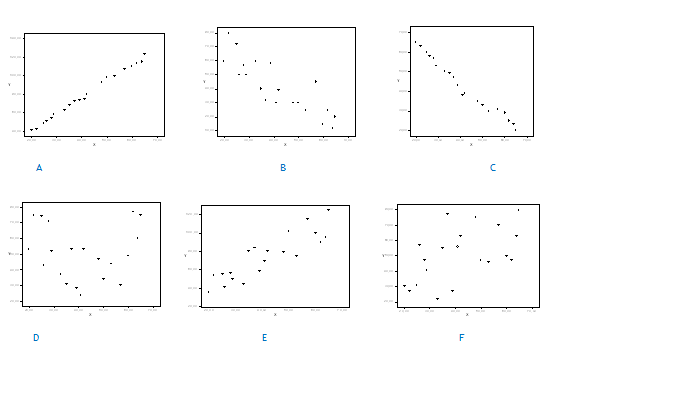
\includegraphics[width=1.10\textwidth]{correlaties.png}
  \captionof{figure}{Correlaties}
  \label{fig:correlaties}
  %\end{figure}
\end{exercise}

\begin{exercise}
  \label{ex:cats}
  Lees het databestand ``Cats.csv'' in. 
  \begin{enumerate}
    \item Voer een lineaire regressieanalyse uit op de variabelen Lichaamsgewicht (\texttt{Bwt}, afhankelijke variabele) en Gewicht hart (\texttt{Hwt}, onafhankelijke variabele).
    \item Maak een spreidingsdiagram van beide variabelen.
    \item Bereken en teken de regressielijn.
    \item Bereken de correlatie- en de determinatiecoëfficiënt.
    \item Geef een interpretatie van deze resultaten.
  \end{enumerate}
\end{exercise}

\begin{exercise}
  \label{ex:cats-per-geslacht}
  Gebruik dezelfde data als in vorige oefening.
  \begin{enumerate}
    \item Voer een lineaire regressieanalyse uit op de variabelen Lichaamsgewicht (Bwt) en Gewicht hart (Hwt) per geslacht.
    \item Maak een spreidingsdiagram van beide variabelen voor elk van de geslachten.
    \item Bereken en teken telkens de regressielijn.
    \item Bereken de correlatie- en de determinatiecoëfficiënt.
    \item Geef een interpretatie aan deze resultaten.
  \end{enumerate}
\end{exercise}

\begin{exercise}
  \label{ex:pizza}
  Lees het databestand ``Pizza.csv'' in.
  \begin{enumerate}
    \item Voer een volledige lineaire regressieanalyse uit op de variabelen Rating en CostPerSlice. Trek hieruit de juiste conclusies en ga deze ook grafisch na.
    \item Onderzoek een mogelijk verband tussen Rating en Neighbourhood. Welke methode kan je hiervoor gebruiken? Kan je de gegevens van Rating hiervoor in dezelfde vorm gebruiken?
    \item Geef een interpretatie aan deze resultaten.
    \item Stel de kruistabel grafisch voor met een staafdiagram.  Voorzie een legende.
  \end{enumerate}
\end{exercise}


%%%%%%%%%%%%%%%%%%%%%%%%%%%%%%%%%%%%%%%%%%%%%%%%%%%%%%



\subsection{Antwoorden op geselecteerde oefeningen}
\label{ssec:analyse-2-variabelen-oplossingen}

\paragraph{Oefening~\ref{ex:muziekwijn-analyse}}

$\chi^2 \approx 18,2792$, Cramér's $V \approx 0,1939$

\paragraph{Oefening~\ref{ex:chisq-survey}}

\begin{enumerate}
  \item \texttt{Exer}/\texttt{Smoke}: $\chi^2 = 5.4885$, $g = 12.59159$, $p = 0.4828422$
  \item \texttt{W.Hnd}/\texttt{Fold}: $\chi^2 = 1.581399$, $g = 5.9915$, $p = 0.454$
  \item \texttt{Sex}/\texttt{Smoke}: $\chi^2 = 3.554$, $g = 7.8147$, $p = 0.314$
  \item \texttt{Sex}/\texttt{W.Hnd}: $\chi^2 = 0.236$, $g = 3.8415$, $p = 0.627$
\end{enumerate}

\paragraph{Oefening~\ref{ex:chisq-aids2}} $\chi^2 = 1083.372914$, $g = 14.067140$, $p \approx 1.157 \times 10^{-229}$

\paragraph{Oefening~\ref{ex:chisq-digimeter}} $\chi^2 \approx 6.6997$ ($df = 6$), $g \approx 12.5916$, $p \approx 0.3495$


\paragraph{Oefening~\ref{oef:casus-akin2016-toets}}

Tabel~\ref{tab:akin2016-resultaten-ttoets} geeft een overzicht met voor elke datasetgrootte het beste en tweede beste persistentietype (op basis van het steekproefgemiddelde). De conclusie van~\textcite{Akin2016}, dat \emph{Realm} het performantste persistentietype is, blijft overeind, maar voor de kleine datasets is het verschil niet significant.

Merk op dat we hier niet expliciet vooraf een significantieniveau gekozen hebben. Voor $\alpha = 0,1$, $0,05$ of zelfs $0,01$, kunnen we echter dezelfde conclusie trekken.

\begin{table}
  \begin{center}
    \begin{tabular}{llll}
      \toprule
      \textbf{Grootte} & \textbf{Beste} & \textbf{2e beste} & \textbf{$p$-waarde} \\ \midrule
      Small            & Realm          & SharedPreferences & 0.1699     \\
      Medium           & Realm          & GreenDAO          & 0.0002506  \\
      Large            & Realm          & SQLite            & 0.0017     \\ \bottomrule
    \end{tabular}
  \end{center}
  \caption{Resultaten $t$-toets voor de beste en 2e beste persistentietype op basis van steekproefgemiddelde~\autocite{Akin2016}.}
  \label{tab:akin2016-resultaten-ttoets}
\end{table}

\paragraph{Oefening~\ref{ex:test-examen}}

\begin{itemize}
  \item $\beta_{0} \approx 0,6333$, $\beta_{1} \approx 0.9667$
  \item $Cov \approx 6,444$, $R \approx 0,9352$, $R^2 \approx 0,8747$
\end{itemize}

\paragraph{Oefening \ref{ex:cats} en \ref{ex:cats-per-geslacht}}

\begin{center}
  \begin{tabular}{lrrrrr}
  	\toprule
    \textbf{Selectie} & \textbf{$\beta_{0}$} & \textbf{$\beta_{1}$} & \textbf{$Cov$} & \textbf{$R$} & \textbf{$R^2$} \\
    \midrule
  	Hele dataset & -0.3511 & 4.0318 & 0.9496 & 0.8041 & 0.6466 \\
  	Female       &  2.9813 & 2.6364 & 0.1979 & 0.5320 & 0.2831 \\
  	Male         & -1.1768 & 4.3098 & 0.9419 & 0.7930 & 0.6289 \\
    \bottomrule
  \end{tabular}
\end{center}


\chapter{Tijdreeksen}
\label{ch:tijdreeksen}

In de voorgaande hoofdstukken hebben we telkens data geanalyseerd die op een bepaald moment in de tijd is verzameld en we hebben uitspraken gedaan over die data voor dat specifieke moment.

In de ict-beroepspraktijk zijn er echter ook vele toepassingen waar het nodig is om data op te volgen die voortdurend verandert. We denken dan bijvoorbeeld aan de belasting van een processor, evolutie van schijfgebruik op een opslagapparaat, de responstijd van een website, enz.

In dit hoofdstuk gaan we dit soort data onder de loep nemen en de belangrijkste analysemethoden bespreken.

\section{Leerdoelen}
\label{sec:tijdreeksen-leerdoelen}

Na dit hoofdstuk moet je in staat zijn om:

\begin{itemize}
  \item Volgende begrippen uit dit hoofdstuk uit te leggen:
  \begin{itemize}
    \item Tijdreeks, voortschrijdend gemiddelde
  \end{itemize}
  \item Gegeven een tijdserie, d.w.z. een reeks observaties van een tijdreeks:
  \begin{itemize}
    \item Het voortschrijdend gemiddelde toepassen;
    \item Op basis van een plot van de observaties inschatten welke vorm van exponentiële afvlakking (enkelvoudige, dubbele, driedubbele/Holt-Winters) het meest geschikt is;
    \item Een voorspelling maken van waarden in de toekomst;
  \end{itemize}
  \item De formules voor voortschrijdend gemiddelde en exponentiële afvlakking te begrijpen en uit te leggen, meer bepaald het effect van de waarde van parameters te kunnen inschatten;
\end{itemize}

\section{Tijdreeksen \& voorspellingen}

\begin{definition}[Tijdreeks]
Een \emph{tijdreeks} is een opeenvolging van observaties van een willekeurige variabele in functie van de tijd.
\end{definition}

Voorbeelden:

\begin{itemize}
	\item maandelijkse vraag naar melk
	\item jaarlijkse instroom van studenten bij de Hogeschool
	\item dagelijks debiet van een rivier
	\item de buitentemperatuur over het verloop van een dag
\end{itemize}

Het voorspellen van tijdreeksen is een belangrijk onderdeel van onderzoek omdat ze vaak de basis vormen voor beslissingsmodellen. Voorbeelden hiervan zijn:

\begin{itemize}
	\item algemene ontwikkeling van toekomstplannen (investeringen, capaciteit \dots)
	\item plannen van budgettering om tekortkomingen te vermijden (operationeel budget, marketing budget \dots)
	\item competitieve leveringstijden van een bedrijf
	\item ondersteuning van financiële objectieven
	\item onzekerheid vermijden
	\item de mogelijkheid om ontwikkelingen in de verkeersveiligheid
kwantitatief te modelleren
\end{itemize}

Tijdreeksen modelleren is een statistisch probleem: we gaan ervan uit dat de observaties variëren volgens een bepaalde kansdichtheidsfunctie in functie van de tijd. Vaak gaan we ervan uit dat de observaties in een tijdreeks gecorreleerd zijn en dus niet uit een willekeurige steekproef komen. 

Er zijn verschillende types modellen in gebruik voor het analyseren van tijdreeksen. Deze modellen hebben met elkaar gemeen dat ze in principe niet alleen de ontwikkeling in een geobserveerde tijdreeks kunnen beschrijven, maar dat we ze ook kunnen gebruiken om

\begin{itemize}
	\item verklaringen te vinden voor die ontwikkeling en
	\item om de toekomstige waarden van de tijdreeks te voorspellen.
\end{itemize}

Hun geschiktheid voor het verwezenlijken van deze doelstellingen loopt echter sterk uiteen. In dit hoofdstuk beperken we ons tot het gebruik van tijdreeksen met een geschiedenis om tijdsafhankelijke modellen te bepalen. Een voorbeeld van een tijdreeks is bijvoorbeeld de leeftijd van de opeenvolgende koningen van Engeland startend van Willem De Veroveraar \autocite{Hipel1994}.

\begin{lstlisting}
kings <- scan(file = 'cursus/data/tijdreeksen/kings.data', skip = 3)
kingstimeseries <- ts(kings)
plot.ts(kingstimeseries, ylab='leeftijd', xlab="tijd")
grid(lty=2,lwd=1,col='black')
\end{lstlisting}

\begin{figure}
	\centering
	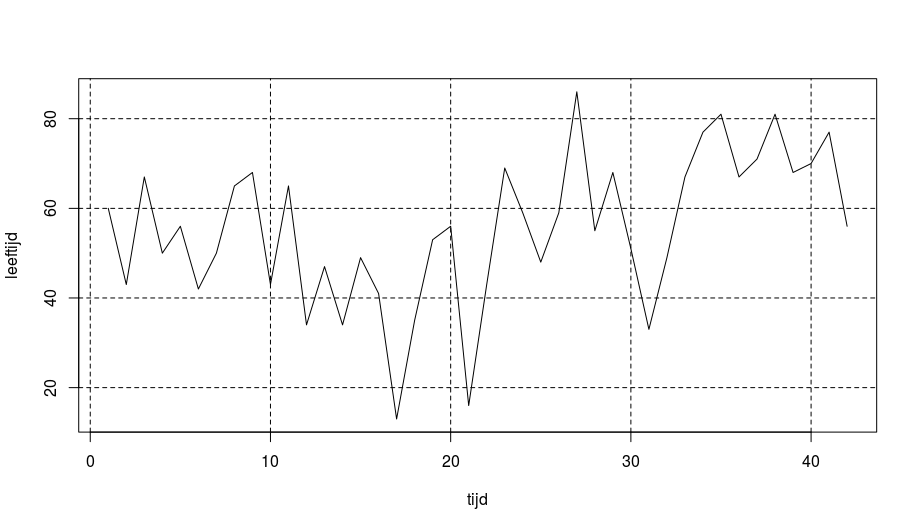
\includegraphics[width=\textwidth]{tijdreeksen/tijdreekskings.png}
	\caption{De tijdreeks die de leeftijden van de koningen voorstelt.}
	\label{fig:tijdreeks11}
\end{figure}

\section{Tijdreeksmodellen}

\subsection{Wiskundig model}

Ons doel is het opstellen van een model dat een verklaring vindt voor de geobserveerde data en dat toelaat om observaties in de toekomst zo goed mogelijk te voorspellen. Het simpelste model dat je kan bedenken is een model waarbij een constante $b$ gebruikt wordt met variaties rond $b$ bepaald door een willekeurige variabele $\epsilon_{t}$ zoals in vergelijking~\ref{eq:constante}. 

\begin{equation}
	X_{t} = b + \epsilon_{t}
\label{eq:constante}
\end{equation}

\begin{description}
  \item [$X_{t}$] stelt een \emph{variabele} voor dat de onbekende is op tijdstip $t$.
  \item [$x_{t}$] stelt een \emph{observatie} voor op tijdstip $t$ (en is dus gekend). 
  \item [$\epsilon_{t}$] noemt met de \emph{storing} (Eng. \emph{noise}) en wordt geacht een gemiddelde van $0$ te hebben met variantie $\sigma^{2}$ en normaal verdeeld ($\epsilon_{t} \sim Nor(0, \sigma)$). 
\end{description}

We kunnen ook ervan uit gaan dat er een lineair verband is:

\begin{equation}
X_{t} = b_{0} + b_{1} \times t + \epsilon_{t}
\label{eq:lineair8}
\end{equation}

De vergelijking in \ref{eq:constante} en \ref{eq:lineair8} zijn speciale gevallen van het polynomiaal geval:

\begin{equation}
	X_{t} = b_{0} + b_{1} t + b_{2} t^{2} + \dots + b_{n} t^{n} + \epsilon_{t} 
\label{eq:polynomiaal}
\end{equation}

\begin{exercise}
	Wat zou volgende tijdreeks kunnen voorstellen?
	\begin{equation}
		X_{t} = b_{0} + b_{1} \sin\left(\frac{2\pi t}{4}\right) + b_{1} \cos\left(\frac{2\pi t}{4}\right) + \epsilon_{t}
	\label{eq:seasonal}
\end{equation}
\end{exercise}

Antwoord: dit is een cyclische tijdreeks met periode $= 4$. Dit zou bijvoorbeeld kunnen gebruikt worden bij een tijdreeks voor seizoenen. 

\begin{lstlisting}
f <- function(a, b,t){
	return(a + b * sin((2 * pi*4)/4) + b * cos((2 * pi*4)/4) + rnorm(1))
}
t <- seq(from = 1, to = 100, by = 1)
X <- lapply(t,f,a=5,b=5)
plot(x = t, y=X, type = 'l')
\end{lstlisting}

\subsubsection{Algemeen}

In elk model beschouwd is de tijdreeks een functie van tijd en parameters van het model. We kunnen algemeen stellen dat:

\begin{equation}
	X_{t} = f(b_{0}, b_{1}, b_{2}, \dots , b_{t}, t) + \epsilon_{t}
\label{eq:general}
\end{equation}

We aanvaarden vervolgens nog volgende stellingen:

\begin{itemize}
	\item Het model gaat uit van twee componenten van variabiliteit: het gemiddelde van de voorspellingen verandert met de tijd en de variaties tot dit gemiddelde variëren willekeurig.
	\item De residuen van het model ($X_{t} - x_{t}$) zijn homoscedastisch : dat wil zeggen in de tijd een constante variantie hebben.
\end{itemize}

Eenmaal het model gekozen, rest enkel nog het  probleem van het schatten van de parameters voor vergelijking \ref{eq:general}. Dit is wat in de volgende stukken besproken zal worden.

\section{Schatten van de parameters}

Eenmaal een model geselecteerd wordt, is het aan de onderzoeker om de parameters te gaan schatten, i.e. parameters die ervoor zorgen dat het model de geobserveerde waarden zo goed mogelijk benaderen. Meestal gaan we ervan uit dat alle waarden gelijkwaardig zijn, maar dat is niet zo bij tijdreeksen. Aangezien onze onafhankelijke parameter de tijd is moeten we methoden bekomen die ervoor zorgen dat recentere data belangrijker zijn dan oude data of omgekeerd. 

In wat volgt beschrijven we de tijdreeksen met geschatte waarden voor de parameters. We duiden schatters aan met een hoedje op de parameters:

\[ \widehat{b}_{1}, \widehat{b}_{2} \dots \widehat{b}_{n} \] 

\subsection{Voortschrijdend gemiddelde}

\begin{table}
\centering
\begin{tabular}{|l|l|l|l|l|l|l|l|l|l|}
  \hline
  4 & 16 & 12 & 25 & 13 & 12 & 4 & 8  & 9 & 14 \\ \hline
  3 & 14 & 14 & 20 & 7  & 9  & 6 & 11 & 3 & 11 \\ \hline
  8 & 7  & 2  & 8  & 8  & 10 & 7 & 16 & 9 & 4  \\ \hline
\end{tabular}
\caption{Voorbeeld van tijdreeksdata, gevisualiseerd in figuur~\ref{fig:tijdreeks21}}
\label{tab:data-tijdreeks21}
\end{table}

Stel dat de statisticus de data in tabel~\ref{tab:data-tijdreeks21} tot het twintigste datapunt beschikbaar heeft (bekende data). De onderzoeker kent de datapunten vanaf het twintigste datapunt niet en moet deze gaan voorspellen. Een eerste model dat gebruikt zou kunnen worden is het constante model zoals in formule~\ref{eq:constante}. 

Volgens dit model worden de datapunten beschouwd als willekeurige waarden uit een populatie met gemiddelde $b$. De beste schatter voor $b$ is het gemiddelde van deze twintig datapunten. 

\begin{lstlisting}
data <- c(4 , 16 , 12 , 25 , 13 , 12 , 4 , 8  , 9 , 14, 
+           3 , 14 , 14 , 20 , 7  , 9  , 6 , 11 , 3 , 11, 
+           8 , 7  , 2  , 8  , 8  , 10 , 7 , 16 , 9 , 4 )
mean(data[1:20])
\end{lstlisting}

\[ \widehat{b} = \frac{1}{20} \sum_{1}^{20} x_{t}= 10.75 \] 

Dit is de beste schatter vertrekkende van de 20 datapunten. We merken wel op dat $x_{1} =  4$ evenveel \textit{waarde} heeft als $x_{20} = 11$, of anders verwoord: de coëfficiënt van $x_{1}$ is dezelfde als die van $x_{20}$, namelijk $\frac{1}{20}$.

Indien we dit als schatter zouden gebruiken dan zien we dat dit in figuur \ref{fig:tijdreeks21} geen goed idee is.

\begin{lstlisting}
AV20 <- matrix(10.75,30,1)
plot.ts(data, col="blue", type='b', xlab='tijd', ylab='Data')
lines(AV20,col='red', type='l')
legend(x= 'topright',legend = c("Data","Average 10.75"), lty = c(1,1), lwd = c(2.5,2.5), col=c('blue','red'))
\end{lstlisting}

\begin{figure}
	\centering
		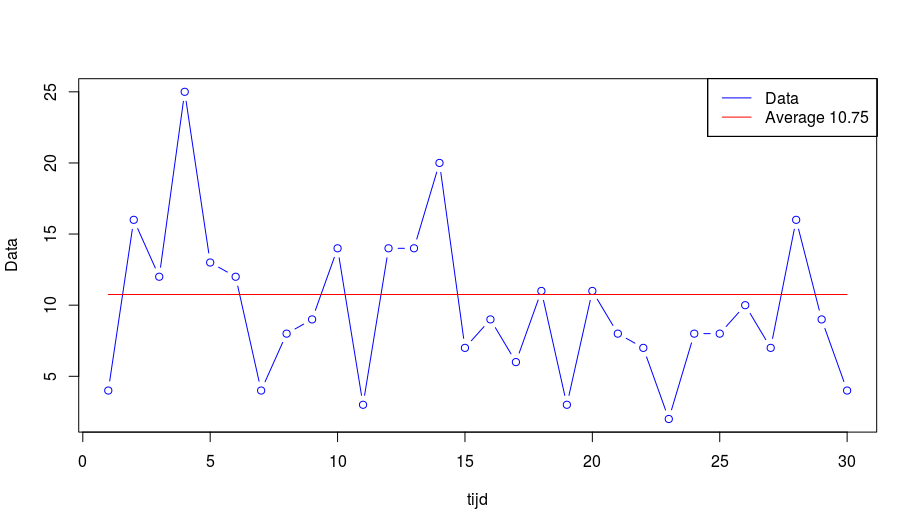
\includegraphics[width=1.00\textwidth]{tijdreeksen/tijdreeks20.png}
	\caption{Tijdreeks met constant gemiddelde $10.75$}
	\label{fig:tijdreeks21}
\end{figure}

Indien we veronderstellen dat de data verandert met de tijd is het beter om oude data minder te laten meetellen dan recentere. Een mogelijkheid is om enkel recente data te gebruiken, bijvoorbeeld de 10 of 5 laatste datapunten (zie figuur \ref{fig:tijdreeks31}).

\[ \widehat{b} = \frac{1}{10} \sum_{10}^{20} x_{t} = 10.18 \] en
\[ \widehat{b} = \frac{1}{5} \sum_{15}^{20} x_{t} = 7.83 \]

\begin{lstlisting}
sma10 <- SMA(x =data,n=10)
sma5 <- SMA(x=data,n=5)
plot.ts(x = data, col = 'blue',type = 'l')
lines(sma10, col='red', type = 'b')
lines(sma5, col='purple', type = 'b')
\end{lstlisting}

\begin{figure}
\centering
	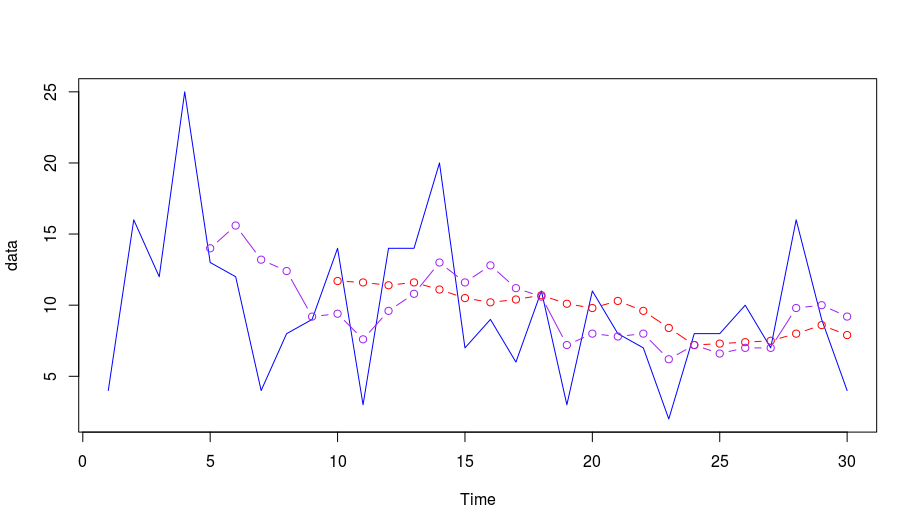
\includegraphics[width=1.00\textwidth]{tijdreeksen/tijdreekssma.png}
	\caption{Tijdreeks met voortschrijdend gemiddelde $m = 10$ en $m=5$}. 
\label{fig:tijdreeks31}
\end{figure}

Dit worden \textit{voortschrijdende gemiddelden}\index{voortschrijdend gemiddelde} genoemd (Eng. \emph{moving average}). 

Welke schatter is nu de beste? We kunnen dit nu nog niet zeggen.

\begin{itemize}
\item De schatter die alle datapunten gebruikt is de beste indien de tijdreeks het model volledig volgt.
\item De schatter met de recentere datapunten is de beste indien de tijdreeks verandert met de tijd.
\end{itemize}

\begin{definition}[voortschrijdend gemiddelde]
Algemeen is het \emph{voortschrijdend gemiddelde} (Eng. \emph{moving average}) het gemiddelde van de $m$ laatste observaties.
\begin{equation}
	\widehat{b} = \sum_{i=k}^{t} \frac{x_{i}}{m}
\label{eq:movingAverage}
\end{equation}
met $k = t-m+1$. $m$ is de time range en is de parameter van de methode.
\end{definition}

\subsection{Meten van de nauwkeurigheid van voorspellingen}

%\begin{table}
%  \centering
%\begin{tabular}{|lllllllllll|}
%
%\end{tabular}
%\caption{Voorspellingsfout voor een moving average $m = 10$}
%\label{tab:error}
%\end{table}

Een methode om de voorspelling te meten is het gemiddelde van de deviaties (Eng.~\emph{Mean Absolute Deviation}, afgekort $MAD$): gemiddelde absolute verschil tussen het voorspelde en de werkelijke waarden van de tijdreeks.

\begin{definition}[$MAD$]
\begin{equation}
	MAD = \frac{1}{n} \sum_{1}^{n} \left| e_{i} \right|  
\label{eq:MAD}
\end{equation}
\end{definition}

Je kan dit ook percenteren om zo tot de gemiddelde absolute procentuele afwijking (Eng.~\emph{Mean Absolute Percentage Error}, afgekort $MAPE$) te komen.

\begin{definition}[$MAPE$]
\begin{equation}
	MAPE = \frac{1}{n} \sum_{1}^{n} \left| \frac{e_{i}}{X_i} \right|  
\label{eq:MAD2}
\end{equation}
\end{definition}

Je kan ook de variantie van de fouten bepalen:

\begin{definition}[$VAR$]
\begin{equation}
	s^{2}_{e} = \frac{1}{m} \sum_{1}^{n} (e_{i} - \overline{e})^{2}
\label{eq:varError}
\end{equation}
\end{definition}

% TODO: moet de noemer hierboven niet n - 1 zijn??

Als laatste interessante parameter kan gekeken worden naar de wortel uit de gemiddelde kwadratische afwijking (Eng.~\emph{root-mean-squared error}, afgekort $RMSE$), als de wortel uit het gemiddelde gekwadrateerde verschil tussen de voorspelde en de werkelijke waarden van de tijdreeks.

\begin{definition}[$RMSE$]
\begin{equation}
	RMSE_{e} = \sqrt{\frac{1}{m} \sum_{1}^{n} (e_{i})^{2}}
\label{eq:varError2}
\end{equation}
\end{definition}

\section{Exponentiële afvlakking}

Bij een voortschrijdend gemiddelde krijgen alle voorgaande observaties een gelijk gewicht. Bij exponentiële afvlakking (Eng. \emph{exponential smoothing}) worden kleinere gewichten toegekend aan oudere observaties. Met andere woorden, recentere observaties krijgen relatief meer gewicht dan oudere observaties.

In het geval van het eenvoudig voortschrijdend gemiddelde zijn de gewichten hetzelfde, namelijk $\frac{1}{m}$.

\subsection{Enkelvoudige exponentiële afvlakking}

Exponentiële afvlakking is een gewogen gemiddelde dat positieve gewichten toekent aan de huidige waarden en waarden uit het verleden van de tijdreeks. Een enkel gewicht, $0\leq \alpha \leq1$ of de afvlakkingsconstante (Eng.~\emph{smoothing constant}) wordt hiervoor gekozen. Voor een tijdseenheid $t$ wordt de enkelvoudige exponentiële afvlakking gevonden door vergelijking \ref{eq:singleExpSmooting}.

\begin{definition}[Exponentiële afvlakking]
\begin{equation}
	X_{t} = \alpha x_{t} + (1-\alpha)X_{t-1}, 0 \leq \alpha \leq 1, t \geq 3
\label{eq:singleExpSmooting}
\end{equation}
\end{definition}

Met andere woorden, $X_{t}$ is een gewogen gemiddelde van de huidige waarneming $x_t$ en de vorige exponentiële afvlakking $X_{t-1}$.

\subsubsection{Intiële setting}
Het bepalen van $X_{2}$ is een belangrijke parameter. Men kan kiezen om:
\begin{enumerate}
	\item $X_{2} = x_{1}$ te stellen
	\item $X_{2}$ gelijk te stellen aan een bepaald objectief
	\item Een gemiddelde te nemen van de eerste $x$ observaties
	\item \dots
\end{enumerate}

Waarom wordt dit een exponentiële methode genoemd? Als we zouden substitueren vinden we bv. voor $X_{t-1}$:

\[ X_{t} = \alpha x_{t} + (1-\alpha)\left[\alpha x_{t-1} + (1-\alpha)X_{t-2}\right] \] 
\[ X_{t} = \alpha x_{t} + \alpha (1-\alpha)x_{t-1} + (1-\alpha)^{2} X_{t-2} \]
of dus algemeen gesteld :
\[ X_{t} = \alpha \sum_{i=0}^{t-2}(1-\alpha)^{i-1}x_{t-i} + (1-\alpha)^{t-2} X_{2}, t \geq 2 \]

Zo merk je dat oudere componenten een exponentieel kleiner gewicht verkrijgen. 

\subsubsection{Waarde voor $\alpha$}
De snelheid waarmee de oude observaties ``vergeten'' worden hangt af van $\alpha$. Met een $\alpha$ dicht bij 1 vergeet je snel, terwijl een $\alpha$ dicht bij nul ervoor zorgt dat vergeten minder snel gaat (zoals aangetoond in tabel \ref{tab:alpha}). Vaak wordt een waarde gebruikt tussen $0.10$ en $0.30$.

\begin{table}
\centering
    \begin{tabular}{l|llll}
    $\alpha$ & $(1-\alpha)$ & $(1-\alpha)^{2}$ & $(1-\alpha)^{3}$ & $(1-\alpha)^{4}$ \\ \hline
    0.9   & 0.1       & 0.01             & 0.001                      & 0.0001           \\
    0.5   & 0.5       & 0.25             & 0.125                      & 0.062            \\
    0.1   & 0.9       & 0.81             & 0.729                      & 0.6561           \\
    \end{tabular}
		\caption{Waarden voor $\alpha$ en $(1-\alpha)^{n}$}
		\label{tab:alpha}
\end{table}

Bijvoorbeeld, het bestand \texttt{precip.data} bevat totale jaarlijkse neerslag in inches voor Londen, vanaf 1813-1912. Laten we dit eens analyseren met R.

\begin{lstlisting}
rain <- scan("cursus/data/tijdreeksen/precip.data",skip=1)
rainseries <- ts(rain,start=c(1813))
plot.ts(rainseries)
plot(rainseriesforecasts)
\end{lstlisting} 

%TODO figuur maken voor verschillende alpha's

\subsubsection{Voorspelling met exponentiële effening}

Stel dat het doel is om de volgende waarde $X_{t+1}$ te voorspellen, dan wordt dit gelijk gesteld aan de afvlakkingswaarde op tijdstip $t$.

\begin{equation}
	X_{t+1} = EMA_t = X_t
	\label{eq:EMA}
\end{equation}

Met $X_t$ de laatst voorspelde waarde. 

We kunnen dit eenvoudig uitvoeren in R. Je krijgt hierbij een \emph{prediction interval}, een interval waarin we verwachten dat de voorspelde waarde met een bepaalde waarschijnlijkheid zal liggen. Standaard krijg je een 80\% en een 95\% interval.

\begin{lstlisting} 
library('forecast')
rainseriesforecasts2 <- forecast.HoltWinters(rainseriesforecasts, h=8)
plot.forecast(rainseriesforecasts2)
\end{lstlisting} 

We zouden correlaties mogen zien tussen de voorspellingsfouten voor opeenvolgende voorspellingen. Met andere woorden, als er sprake is van een correlatie tussen prognosefouten voor opeenvolgende voorspellingen, is het eerder waarschijnlijk dat de simpele exponentiële afvlakking kan worden verbeterd door een andere voorspellingstechniek te gebruiken.

Om te achterhalen of dit het geval is, kunnen we een correlogram verkrijgen van de in-sample voorspellingsfouten voor.

We weten nog uit hoofdstuk~\ref{ch:analyse2var} dat de covariantie of correlatie de lineaire relatie beschrijft tussen twee variabelen. De autocovariantie en autocorrelatie meten de lineaire relatie tussen in de tijd verschoven waarden voor een tijdreeks.

\begin{definition}[Autocovariantie]
	We definiëren de autocovariantie bij vertraging $k$ door $c_k$.
	\[ c_k = \sum_{t=k+1}^{T} (y_t - \overline{y})(y_{t-k} - \overline{y}) \]
\end{definition}

\begin{definition}[Autocorrelatie]
	We definiëren de autocorrelatie bij vertraging $k$ door $r_k$.
	\[ r_k = \frac{c_k}{c_0} \]
\end{definition}

Een correlogram is een grafiek van de autocorrelaties. In R kan je die plotten met de functie \texttt{acf()}. Deze berekent ook de voorspellingsfouten. Om de maximale vertraging te bepalen die we willen bekijken, gebruiken we de parameter \texttt{lag.max}.

Bijvoorbeeld, om een correlogram te berekenen van de prognosefouten voor de Londen-regenvalgegevens voor vertragingen 1 tot en met 20, typen we:

\begin{lstlisting}
acf(rainseriesforecasts2$residuals, lag.max=20, na.action = na.pass)
\end{lstlisting}

Om te testen of er significant bewijs is voor significante correlaties bij vertraging 1-20, kunnen we een Ljung-Box test uitvoeren. Dit kan in R worden gedaan met de functie \texttt{Box.test()}. De maximale vertraging die we willen bekijken, wordt gespecificeerd met behulp van de parameter \texttt{Lag}.

De test volledig uitleggen valt buiten het bereik van deze cursus, maar de test gaat uit van de hieronder geformuleerde hypothesen $H_0$ en $H_1$. De teststatistieken kunnen dan gewoon geïntepreteerd worden zoals alle andere hypothesetesten die beschreven geweest zijn in vorige hoofdstukken. 

\begin{itemize}
  \item $H_0$ De gegevens zijn onafhankelijk verdeeld (d.w.z. de correlaties in de populatie waaruit de sample wordt genomen, zijn 0, zodat elke waargenomen correlatie in de data voortvloeien uit willekeurigheid).
  \item $H_1$ De gegevens zijn niet onafhankelijk verdeeld: ze tonen een linaire correlatie.
\end{itemize}

Bijvoorbeeld, om te testen of er geen nul autocorrelaties zijn op vertragingen 1-20, voor de in-sample voorspellingen fouten voor Londen regenval data, typen we:

% TODO: correcte Nl term voor in-sample error?

\begin{lstlisting}
Box.test(rainseriesforecasts2$residuals, lag=20, type="Ljung-Box")
Box-Ljung test
data:  rainseriesforecasts2$residuals
X-squared = 17.4008, df = 20, p-value = 0.6268
\end{lstlisting}

Als laatste moeten we ook kijken naar de verdeling van de fouten van de voorspelling. Zoals boven vermeld gaan we ervan uit dat de fouten normaal verdeeld zijn met een gemiddelde $\mu = 0$ en een standaardafwijking die constant is. Om deze veronderstelling te controleren, kunnen we een histogram van de prognosefouten plotten, met een overlappende normale curve met gemiddelde nul en dezelfde standaardafwijking heeft als de verdeling van de voorspellingsfouten. Hiervoor kunnen we een R-functie \texttt{plotForecastErrors()} definiëren. Het is ook aangewezen de methoden zoals beschreven in sectie~\ref{sec:normtesting}.

% TODO: zin onvolledig

\begin{lstlisting}
plotForecastErrors <- function(forecasterrors)
{
# make a histogram of the forecast errors:
mybinsize <- IQR(forecasterrors)/4
mysd   <- sd(forecasterrors)
mymin  <- min(forecasterrors) - mysd*5
mymax  <- max(forecasterrors) + mysd*3
# generate normally distributed data with mean 0 and standard deviation mysd
mynorm <- rnorm(10000, mean=0, sd=mysd)
mymin2 <- min(mynorm)
mymax2 <- max(mynorm)
if (mymin2 < mymin) { mymin <- mymin2 }
if (mymax2 > mymax) { mymax <- mymax2 }
# make a red histogram of the forecast errors, with the normally distributed data overlaid:
mybins <- seq(mymin, mymax, mybinsize)
hist(forecasterrors, col="red", freq=FALSE, breaks=mybins)
# freq=FALSE ensures the area under the histogram = 1
# generate normally distributed data with mean 0 and standard deviation mysd
myhist <- hist(mynorm, plot=FALSE, breaks=mybins)
# plot the normal curve as a blue line on top of the histogram of forecast errors:
points(myhist$mids, myhist$density, type="l", col="blue", lwd=2)
}
\end{lstlisting}

\subsection{Dubbele exponentiële afvlakking}

Enkelvoudige afvlakking wordt gebruikt wanneer er geen trend zichtbaar is. Wanneer er een trend (stijgend of dalend) is dan kan er iets fout gaan. Zie bijvoorbeeld de data in tabel~\ref{tab:trend} en figuur~\ref{fig:tijdreeks61}.

\begin{table}
\centering
    \begin{tabular}{|ll|}
    \hline
    Data & Enkelvoudige afvlakking \\
    6.4  & ~                      \\
    5.6  & 6.4                    \\
    7.8  & 6.2                    \\
    8.8  & 6.7                    \\
    11.0 & 7.3                    \\
    11.6 & 8.4                    \\
    16.7 & 9.4                    \\
    15.3 & 11.6                   \\
    21.6 & 12.7                   \\
    22.4 & 15.4                   \\ \hline
    \end{tabular}
		\caption{Enkelvoudige afvlakking met $\alpha = 0.3$}
		\label{tab:trend}
\end{table}

\begin{figure}
  \centering
  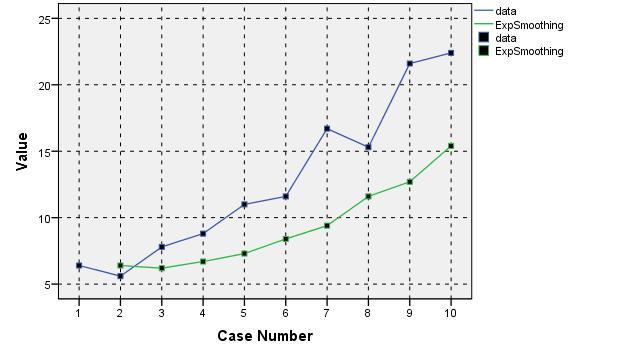
\includegraphics[width=1.00\textwidth]{tijdreeksen/tijdreeks61.jpg}
  \caption{Exponentiële afvlakking bij een trend}
  \label{fig:tijdreeks61}
\end{figure}

Daarom voegen we een extra constante toe om deze trap te overbruggen:

\begin{definition}[Holt-voorspelling of dubbele exponentiële afvlakking]
\begin{eqnarray}
	X_{t} = \alpha x_{t} + (1-\alpha)(X_{t-1} + b_{t-1}) & 0 \leq \alpha \leq 1 \\
	b_{t} = \beta(X_{t}-X_{t-1}) + (1-\beta)b_{t-1} & 0 \leq \beta \leq 1 
\label{eq:doubleSmoothing}
\end{eqnarray}
\end{definition}

\subsubsection{Initiële waarde}

Net zoals in enkelvoudige afvlakking kan je verschillende methodes kiezen om initiële waardes voor $X_{t}$ en $b_{t}$ te kiezen:

\begin{itemize}
	\item $X_{1} = x_{1}$
	\item $b_{1} = x_{2} - x_{1}$
	\item $b_{1} = \frac{1}{3}\left[ (x_{2} - x_{1}) + (x_{1} - x_{2}) + (x_{4} - x_{3}) \right]$
	\item $b_{1} = \frac{x_{n} - x_{1}}{n-1}$
\end{itemize}

\subsubsection{Voorspelling}

Een voorspelling maken met dubbele exponentiële afvlakking gebeurt dan iets anders (noem $F_{t+1}$ de voorspelling voor tijd $T+1$):

\[ F_{t+1} = X_{t} + b_{t} \]
of
\[ F_{t+m} = X_{t} + m b_{t} \]

Als we nu de tekening maken met enkelvoudige afvlakking ($\alpha = 0.977$) en dubbele afvlakking ($\alpha = 0.3623, \beta = 1.0, X_{1} = x_{1} = 6.4$ en $b_{1} = \frac{1}{3}\left[ (x_{2} - x_{1}) + (x_{1} - x_{2}) + (x_{4} - x_{3}) \right] = 0.8$) vinden we volgende waarden in tabel \ref{tab:doubleSingle} en figuur \ref{fig:tijdreeks71}:

\begin{table}
  \centering
  \begin{tabular}{|llll|}
    \hline
    Data & Enkelvoudige afvlakking $X_{t}$ & Dubbele afvlakking $X_{t}$ & $F_{t}$ \\
    6.4  & ~                      & 6.4              & ~                             \\
    5.6  & 6.4                    & 6.6              & 7.2                           \\
    7.8  & 5.6                    & 7.2              & 6.8                           \\
    8.8  & 6.7                    & 8.1              & 7.8                           \\
    11.0 & 8.8                    & 9.8              & 9.1                           \\
    11.6 & 10.9                   & 11.5             & 11.4                          \\
    16.7 & 11.6                   & 14.5             & 13.2                          \\
    15.3 & 16.6                   & 16.7             & 17.4                          \\
    21.6 & 15.3                   & 19.9             & 18.9                          \\
    22.4 & 21.5                   & 22.8             & 23.1                          \\ \hline
  \end{tabular}
  \caption{Tabel met enkelvoudige en dubbele afvlakking}
  \label{tab:doubleSingle}
\end{table}

\begin{figure}
	\centering
		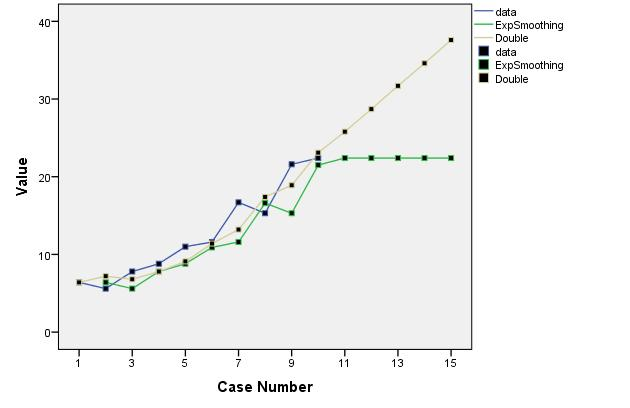
\includegraphics[width=1.00\textwidth]{tijdreeksen/tijdreeks71.jpg}
	\caption{Enkelvoudige en dubbele afvlakking}
	\label{fig:tijdreeks71}
\end{figure}

De manier om dit met R op te lossen is gelijkaardig als bij exponentiële afvlakking, alleen moet de parameter gamma $\beta$ niet op NULL gezet worden. Het maken van de correlogram, de Ljung–Box test en het testen van de normaliteit van de errors gebeurt om dezelfde manier. 

\subsection{Driedubbele exponentiële afvlakking}

In vele tijdreeksen zie je bepaalde patronen terugkomen. Neem bijvoorbeeld is de dagelijkse omzet van een bakker: die zal elke dag anders zijn, maar als je die over een lange periode bekijkt, zal je wellicht elke week een gelijkaardig patroon terugzien (met bv. een topomzet op zondag).

Dit soort tijdreeksen kan benaderd worden met de Holt-Winters methode, of driedubbele exponentiële afvlakking.

\begin{eqnarray}
  X_{t} = \alpha \frac{x_{t}}{c_{t-L}} + (1-\alpha) (X_{t-1} + b_{t-1}) & \textnormal{Smoothing}\\
  b_{t} = \beta (X_{t} - X_{t-1}) + (1-\beta)b_{t-1} & \textnormal{Trend smoothing} \\
  c_{t} = \gamma \frac{x_{t}}{X_{t}} + (1-\gamma)c_{t-L} & \textnormal{Seasonal smoothing} \\
  F_{t+m} = (X_{t} + mb_{t})c_{t-L+m \mod L}  & \textnormal{Voorspelling}
  \label{eq:HoltWinters}
\end{eqnarray}
 met 
\begin{itemize}
	\item $x_{t}$ de observatie op tijdstip $t$
	\item $X_{t}$ is de afgevlakte observatie op tijdstip $t$
	\item $b_{t}$ is de trendfactor op tijdstip $t$
	\item $c_{t}$ is de seizoensindex op tijdstip $t$
	\item $F_{t}$ is de voorspelling op tijdstip $t$
	\item $L$ is de periode (bv. van de seizoenen)
\end{itemize}

$\alpha, \beta en \gamma$ zijn constanten die geschat moeten worden. 
De manier om dit met R op te lossen is gelijkaardig als bij exponentiële afvlakking. Het maken van de correlogram, de Ljung–Box test en het testen van de normaliteit van de errors gebeurt op dezelfde manier. 

\section{Oefeningen}
\label{sec:tijdreeksen-oefeningen}

\begin{exercise}
In bijgevoegd bestand \emph{Budget.csv} vind je vanaf 1981 tot 2005 per kwartaal de omzet, het advertentiebudget en het BNP van een middelgroot bedrijf. Voeg zelf nog een kolom 'Kwartaalnummer' toe.

\begin{enumerate}
  \item Bereken het voortschrijdend gemiddelde \emph{(simple moving average)} over de periodes 4 en 12 voor deze data. Gebruik hiervoor de methode SMA. Maak een lijngrafiek van $X$, $SMA(4)$ en $SMA(12)$.
  \item Welke techniek die we eerder gezien hebben (in het deel over beschrijvende statistiek) is ook geschikt om voorspellingen te maken over de waarden van $X$? Werk dit uit aan de hand van de daarvoor bestemde functie en plot het resultaat in de grafiek.
  \item Gebruik de methode \emph{forecast} om voorspellingen voor de 10 volgende periodes met elk van voorgaande methoden (dus moving average 4 en 10 en regressie) te maken. Teken deze eveneens op de grafiek.
  \item Is het gebruik van één van deze technieken interessant om voor deze data voorspellingen te maken? 
  \item Maak van de data een tijdreeks via de methode \emph{ts}. Gebruik de methode \emph{decompose} om de tijdreeks op te delen en zo een idee te krijgen van de trend en de seizoenschommeling.
  \item Bereken het exponentieel voortschrijdend gemiddelde \emph{(exponential moving average, EMA)} door gebruik te maken van de methode \emph{HoltWinters}. Maak opnieuw via de methode \emph{forecast} een voorspelling voor 20 periodes. Gebruik als startwaarden $s_1 = x_1$ en $\alpha $ de door R gegenereerde waarde. Plot het resultaat op een nieuwe grafiek samen met $X$.
  \item Doe nu hetzelfde met $\alpha=0.1$. 
  \item Hoe zien de voorspellingen er nu uit?
  \item Doe nu hetzelfde met \emph{dubbele} exponentiële afvlakking. Gebruik als startwaarden $s_1 = x_1$ en $b_1 = \frac{x_n - x_1}{n - 1}$, $\alpha =  0.05$ en $\beta = 0.2$. Plot het resultaat op de grafiek.
  \item Gebruik dubbele exponentiële afvlakking om voorspellingen te berekenen voor 20 periodes. Plot de waarden op de grafiek. Is deze techniek beter of slechter dan de vorige voor deze dataset?
  \item Speel met de waarden voor $\alpha$ en $\beta$ en bekijk het resultaat, zowel voor enkele als dubbele exponentiële afvlakking.
  \item Gebruik de \emph{HoltWinters}-methode zonder trend.  M.a.w. we stellen $\beta=0$. Gebruik als startwaarden $\alpha =  0.05$ en $\gamma = 0.9$. Plot het resultaat op de grafiek.
  \item Bereken opnieuw voorspellingen voor 20 periodes. Plot de waarden op de grafiek. Is deze techniek beter of slechter dan de vorige voor deze dataset?
  \item Speel met de waarden voor $\alpha$, $\beta$ en $\gamma$ en bekijk het resultaat.
  \item Gebruik de \emph{HoltWinters}-methode met de door R-gegeneerde waarden zonder trend.  M.a.w. we stellen $\beta=0$.  Plot het resultaat op de grafiek.
  \item Bereken opnieuw voorspellingen voor 20 periodes maar gebruik nu de methode \emph{predict}. Plot de waarden op de grafiek. Is deze techniek beter of slechter dan de vorige voor deze dataset?
\end{enumerate}	
\end{exercise}

\begin{exercise}
In bestand \emph{Passagiers2.csv} vind je vanaf januari 1949 tot december 1960 het aantal passagiers van een luchtvaartmaatschappij. 
\begin{enumerate}
  \item Bereken het voortschrijdend gemiddelde \emph{(simple moving average)} over de periodes 4 en 12 voor deze data. Gebruik hiervoor de methode \emph{ma}. Maak een lijngrafiek van $X$, $MA(4)$ en $MA(12)$.
  \item Welke techniek die we eerder gezien hebben (in het deel over beschrijvende statistiek) is ook geschikt om voorspellingen te maken over de waarden van $X$? Werk dit uit aan de hand van de daarvoor bestemde functie en plot het resultaat in de grafiek.
  \item Gebruik de methode \emph{forecast} om voorspellingen voor de 10 volgende periodes met elk van voorgaande methoden (dus moving average 4 en 12 en regressie) te maken. Teken deze eveneens op de grafiek. Conclusie?
  \item Is het gebruik van één van deze technieken interessant om voor deze data voorspellingen te maken? 
  \item Gebruik de methode \emph{decompose} om de tijdreeks op te delen en zo een idee te krijgen van de trend en de seizoenschommeling.
  \item Bereken het exponentieel voortschrijdend gemiddelde \emph{(exponential moving average, EMA)} door gebruik te maken van de methode \emph{ses} met $\alpha=0.2$. Maak opnieuw via de methode \emph{forecast} een voorspelling voor 20 periodes. Plot het resultaat op een nieuwe grafiek samen met $X$.
  \item Doe nu hetzelfde met $\alpha=0.6$ en $\alpha=0.89$. 
  \item Hoe zien de voorspellingen er nu uit?
  \item Doe nu hetzelfde met \emph{dubbele} exponentiële afvlakking. Gebruik hiervoor de methode \emph{holt}  $\alpha =  0.8$ en $\beta = 0.2$. Plot het resultaat op de grafiek.
  \item Gebruik dubbele exponentiële afvlakking om voorspellingen te berekenen voor 20 periodes. Plot de waarden op de grafiek. Is deze techniek beter of slechter dan de vorige voor deze dataset?
  \item Gebruik in de methode de optie $exponential=TRUE$. Teken het resultaat.  Wat is het verschil?
  \item Gebruik de \emph{hw}-methode met de door R gegeneerde waarden. Plot het resultaat op de grafiek.
  \item Bereken opnieuw een aantal voorspellingen via de methode \emph{predict}. Plot de waarden op de grafiek. Is deze techniek beter of slechter dan de vorige voor deze dataset?
  \item Speel met de waarden voor $\alpha$, $\beta$ en $\gamma$ en bekijk het resultaat.
\end{enumerate}

\end{exercise}


\begin{appendices}
%\chapter{Logistisch regressie}

\section{Inleiding}

In dit onderzoek gaan we een andere vorm van verband zoeken tussen variabelen waarbij de afhankelijke variabele twee waarden kan aannemen. 

\begin{example}
	\label{ex:slagen}
	Stel dat je wil nagaan of het student al dan niet zal slagen voor het examen onderzoekstechnieken. We zijn dus ge\"interesseerd in de voorspelling (door
	onafhankelijke variabelen) van de kans dat een student in de categorie 'examen slagen' of in de categorie 'niet slagen' valt. 
\end{example}

In bovenstaand voorbeeld zal een 'gewone' lineaire regressie analyse 
algemeen wel de juiste richting van de $\beta$-co\"efficiënten opleveren. Maar de schatting is niet helemaal correct, omdat enkele belangrijke regressie assumpties geschonden worden, zoals de normaliteitsassumptie en de assumptie van homoscedasticiteit. Het grootste probleem is evenwel dat de door lineaire regressie voorspelde kansen groter kunnen zijn dan 1 en kleiner dan 0 en dat is niet te interpreteren.

Bij logistische regressie gaan we werken met kansverhoudingen. In voorbeeld \ref{ex:slagen} hebben we een kansverdeling dat een student wel slaagt $p$ gedeeld door de kans om niet te slagen $1-p$:
\[ 
	\textnormal{verhouding} = \frac{p}{1-p}
\]

We wensen dat de waarden van de verhouding gaan van $- \infty$ tot $\infty$ gaan. Daarom gaan we de natuurlijke logaritme nemen van de verhouding. Om de functie te tekenen van de logaritmische functie kan je onderstaande code gebruiken. 

\lstinputlisting{data/logcurve.R}

Als we de onafhankelijke variabelen $X_1$, $X_2$  \dots $X_n$ noemen,dan ziet het logistische model er in formulevorm als volgt uit:
\[ 
	log(\frac{p}{1-p}) = \beta_0 + \beta_1 X_1 + \cdots + \beta_n X_n 
\]

We kunnen het kansmodel ook herschrijven (afzonderen van de p):

\[ 
	p = \frac{e^{\beta_0 + \beta_1 X_1 + \cdots + \beta_n X_n }}{1+ e^{\beta_0 + \beta_1 X_1 + \cdots + \beta_n X_n }}
\]

We kunnen het kansmodel dan ook herschrijven (afzonderen van de $(1-p)$):
\[ 
1-p = \frac{1}{1+ e^{\beta_0 + \beta_1 X_1 + \cdots + \beta_n X_n }}
\]
Aan deze formules is af te lezen dat de kansen $p$ en $1-p$ bij elkaar opgeteld gelijk zijn aan \'e\'en.
Verder is te zien dat de kansen $p$ en $1-p$ afhankelijk zijn van de variabelen $X_1, X_2 \cdots X_n$, maar dat deze afhankelijkheid niet lineair is. Een logistische regressielijn ziet er dus niet als een rechte lijn
uit, maar als een S-vormige curve. (TODO: hier zou een tekening moeten komen van de sigmo\"ide functie).

Bij logistische regressie gaan we dus op zoek naar goede waarden voor $\beta_0 \cdots \beta_n$. Dit kan in R makkelijk door de methode \texttt{glm}.

\section{Logistische regressie in R}

We gaan het voorbeeld nemen dan in Kaggle \footnote{\href{https://www.kaggle.com/c/titanic/data}{https://www.kaggle.com/c/titanic/data}} gegeven wordt. Het bevat de informatie rond de mensen die de reis van de titanic ondernomen hebben en het overleefd hebben of niet. De analyse komt uit het blog artikel \cite{michy}

\subsection{Data cleaning}

We gaan de data opruimen en kijken welke parameters er in het model kunnen zitten. We gaan dit na door te kijken welke parameters in de dataset niet voldoende aanwezig zijn. 

\begin{lstlisting}
sapply(train,function(x) sum(is.na(x)))
sapply(train, function(x) length(unique(x)))
missmap(train, main = "Missing values vs observed")
\end{lstlisting}
Hierbij zien we dat de variabelen \texttt{cabin} te weinig waarden bevat. Ook \texttt{tickets} laten we vallen aangezien dit weinig invloed zal hebben. 
 We nemen dus een subset van de data en gaan hiermee aan de slag. 
 
 


\chapter{Notatie}
\label{app:notatie}

\begin{table}
  \centering
  \begin{tabular}{p{.25\textwidth}p{.75\textwidth}}
  	\toprule
  	\textbf{Notatie}                                        & \textbf{Betekenis}                                                                                                                     \\
  	\midrule
  	$\widehat{a}, \widehat{b}, \ldots$                      & Het ``hoedje'' geeft aan dat het gaat om een schatter.                                                                                 \\
  	$d \in \mathbb{R}$                                      & Effectgrootte, of Cohen's $d$                                                                                                          \\
  	$M \sim Nor(\mu_{\overline{x}}, \sigma_{\overline{x}})$ & De kansverdeling van het steekproefgemiddelde (cfr.~de centrale limietstelling, Sectie~\ref{sec:centrale-limietstelling})              \\
  	$N \in \mathbb{N}$                                      & De populatiegrootte                                                                                                                    \\
  	$n \in \mathbb{N}$                                      & De steekproefgrootte                                                                                                                   \\
  	$p \in [0, 1]$                                          & Een kans, of specifiek de overschrijdingskans in een statistische toets.                                                               \\
  	$R \in [-1, +1]$                                        & Pearson's product-momentcorrelatiecoëfficiënt (kort: correlatiecoëfficiënt). In de literatuur soms ook $\rho$ (rho).                   \\
  	$R^2 \in [0, 1]$                                        & Determinatiecoëfficiënt. In de literatuur soms ook $\rho^2$.                                                                           \\
  	$s$                                                     & De standaardafwijking van een steekproef                                                                                               \\
  	$s^2$                                                   & De variantie van een steekproef                                                                                                        \\
  	$t \in \mathbb{N}$                                      & Een tijdstip                                                                                                                           \\
  	$X = \left\{x_1, x_2, \ldots, x_n \right\}$             & Een stochastische variabele $X$ met $n$ waarnemingen $x_i$ (voor $i: 1 \ldots n$)                                                      \\
  	$X \sim Nor(\mu, \sigma)$                               & De variabele $X$ is \emph{normaal verdeeld} met gemiddelde $\mu$ en standaardafwijking $\sigma$                                        \\
  	$\overline{x}$                                          & Het gemiddelde over de \emph{steekproef}                                                                                               \\
  	$Z \sim Nor(0, 1)$                                      & $Z$ is een variabele met een kansverdeling die de \emph{standaardnormaalverdeling} volgt, dus met gemiddelde 0 en standaardafwijking 1 \\
  	\midrule
  	$\alpha$ (alfa)                                         & Een significantieniveau (voor een statistische toets)                                                                                  \\
  	$1 - \alpha$                                            & Een betrouwbaarheidsniveau (voor een betrouwbaarheidsinterval)                                                                         \\
  	$\epsilon$                                              & Storing in een tijdreeks (typisch een klein getal)                                                                                     \\
  	$\mu$ (mu)                                              & Het gemiddelde (ook: verwachtingswaarde) over heel de \emph{populatie}.                                                                \\
  	$\mu_{\overline{x}}$                                    & De verwachtingswaarde bij de kansverdeling van het steekproefgemiddelde                                                                \\
  	$\sigma$ (sigma)                                        & De standaardafwijking over heel de populatie                                                                                           \\
  	$\sigma^2$                                              & De variantie over heel de populatie                                                                                                    \\
  	$\sigma_{\overline{x}}$                                 & De standaardafwijking bij de kansverdeling van het steekproefgemiddelde                                                                \\
  	\bottomrule
  \end{tabular}
  \caption[Overzicht gebruikte symbolen.]{\textbf{Overzicht gebruikte symbolen.} De symbolen zijn alfabetisch gesorteerd, met eerst het latijnse en daarna het Griekse alfabet (zie Tabel~\ref{tab:griekse-alfabet}).}
  \label{tab:notatie}
\end{table}

\begin{table}
  \centering
  \begin{tabular}{lll}
  	\toprule
  	\textbf{Grieks}              & \textbf{Naam} & \textbf{Klank, uitspraak}   \\
  	\midrule
  	$A, \alpha$                  & alfa          & a                           \\
  	$B, \beta$                   & bèta          & b                           \\
  	$\Gamma, \gamma$             & gamma         & g                           \\
  	$\Delta, \delta$             & delta         & d                           \\
  	$E, \epsilon$                & epsilon       & e                           \\
  	$Z, \zeta$                   & zèta          & dz                          \\
  	$H, \eta$                    & èta           & ei                          \\
  	$\Theta, \theta$             & thèta         & th                          \\
  	$I, \iota$                   & iota          & i                           \\
  	$K, \kappa$                  & kappa         & k                           \\
  	$\Lambda, \lambda$           & lambda        & l                           \\
  	$M, \mu$                     & mu            & m                           \\
  	$N, \nu$                     & nu            & n                           \\
  	$\Xi, \xi$                   & xi            & ks                          \\
  	$O, o$                       & omikron       & o (kort)                    \\
  	$\Pi, \pi$                   & pi            & p                           \\
  	$P, \rho$                    & rho           & r                           \\
  	$\Sigma, \sigma (\varsigma)$ & sigma         & s                           \\
  	$T, \tau$                    & tau           & t                           \\
  	$\Upsilon, \upsilon$         & upsilon       & u                           \\
  	$\Phi, \phi (\varphi)$       & phi           & f                           \\
  	$X, \chi$                    & chi           & ch (zoals in \emph{chemie}) \\
  	$\Psi, \psi$                 & psi           & ps                          \\
  	$\Omega, \omega$             & omega         & o (lang)                    \\
  	\bottomrule
  \end{tabular}
  \caption[Het Griekse alfabet]{\textbf{Het Griekse alfabet.} In wiskundige en statistische teksten worden vaak Griekse letters gebruikt. Ter info vind je hier een overzicht van het Griekse alfabet. Telkens is de hoofd- en kleine letter gegeven. Soms staat tussen haakjes een variant van de letter die soms ook voorkomt.}
  \label{tab:griekse-alfabet}
\end{table}

\clearpage
\addcontentsline{toc}{chapter}{\textcolor{maincolor}{\IfLanguageName{dutch}{Bibliografie}{Bibliography}}}
\printbibliography

\clearpage
\addcontentsline{toc}{chapter}{\textcolor{maincolor}{Index}}
\printindex

\end{appendices}
\end{document}
